% Giacomo version
\documentclass[a4paper,11pt]{report}

% --- Essential packages ---
\usepackage{helvet}
\renewcommand{\familydefault}{\sfdefault}
\usepackage[T1]{fontenc}
\usepackage[utf8]{inputenc}    
\usepackage{geometry}
\geometry{margin=1in}
\usepackage{comment}
\usepackage{graphicx}
\usepackage{amsmath}
\usepackage{booktabs}
\usepackage{listings}
\usepackage{float}
\usepackage[usenames,dvipsnames]{xcolor}
\usepackage{tikz}
\usetikzlibrary{automata, positioning, arrows.meta, fit, shapes.geometric}
\usepackage{pgfplots}
\usepackage{subcaption}
\usepackage{longtable}
\usepackage{array}
\usepackage{booktabs}
\usepackage{tabularx}
\usepackage{siunitx}
\usepackage{todonotes}
\usepackage{hyperref}
\usepackage{multirow}


%--------------------------------------------------
% include pdf in latex
%--------------------------------------------------
\usepackage{pdfpages}

%--------------------------------------------------
% BOM Table
%--------------------------------------------------

\usepackage{ragged2e}    % for \RaggedRight in p{} columns
\usepackage{eurosym}     % for \euro symbol

%--------------------------------------------------
% Document formatting
%--------------------------------------------------

\usepackage{caption}
\captionsetup{
    labelfont=bf,
    textfont=bf
}

\newcommand{\tableicon}[1]{%
    \raisebox{-0.35\height}{\includegraphics[height=5mm]{#1}}%
}

% chapter package
\usepackage{titlesec}
\titleformat{\chapter}
  {\normalfont\Huge\bfseries}
  {Chapter \thechapter.}
  {0.5em}
  {}
\titlespacing*{\chapter}{0pt}{-10pt}{20pt}

% date format extra command
\makeatletter
\newcommand{\todayNum}{%
  \the\year-\two@digits{\month}-\two@digits{\day}}
\makeatother

% Bibliography management
% Note: this document uses biblatex with backend=biber.
% Build this project with latexmk so bibliography updates are applied automatically.
% Use either: latexmk -pdf main.tex or build.bat
\usepackage[backend=biber,style=ieee]{biblatex}
\addbibresource{references.bib}

%-------------------------------------------------
% -------------- Requirements Package ------------
%-------------------------------------------------
\usepackage{lmodern}
\usepackage{colortbl}
\newcolumntype{L}[1]{>{\raggedright\arraybackslash}m{#1}}
\definecolor{tablehead}{gray}{0.6}
\definecolor{tablecat}{gray}{0.8}
\definecolor{tablereq}{RGB}{230, 235, 240}


\renewcommand{\arraystretch}{1.3}

% Requirement numbering
\newcounter{req}
\newcounter{reqsub}[req]
\newcounter{reqsubsub}[reqsub]
\renewcommand{\thereq}{R-\arabic{req}}
\renewcommand{\thereqsub}{R-\arabic{req}.\arabic{reqsub}}
\renewcommand{\thereqsubsub}{R-\arabic{req}.\arabic{reqsub}.\arabic{reqsubsub}}

\newcommand{\Req}[1]{\refstepcounter{req}\label{#1}\thereq}
\newcommand{\ReqSub}[1]{\refstepcounter{reqsub}\label{#1}\thereqsub}
\newcommand{\ReqSubSub}[1]{\refstepcounter{reqsubsub}\label{#1}\thereqsubsub}

\newcommand{\categoryrow}[2]{%
  \multicolumn{1}{>{\columncolor{tablecat}}L{1cm}}{} &%
  \multicolumn{1}{>{\columncolor{tablecat}}L{1.5cm}}{#1} &%
  \multicolumn{1}{>{\columncolor{tablecat}}L{12.5cm}}{#2} \\
}

\newcommand{\requirementrow}[2]{%
  \multicolumn{1}{>{\columncolor{tablereq}}L{1cm}}{} &%
  \multicolumn{1}{>{\columncolor{tablereq}}L{1.5cm}}{#1} &%
  \multicolumn{1}{>{\columncolor{tablereq}}L{12.5cm}}{#2} \\
}

\newcommand{\headerrow}{%
  \multicolumn{1}{>{\columncolor{tablehead}}L{1cm}}{Resp.} &%
  \multicolumn{1}{>{\columncolor{tablehead}}L{1.5cm}}{ID} &%
  \multicolumn{1}{>{\columncolor{tablehead}}L{12.5cm}}{Description} \\
}

%-------------------------------------------------
% -------------- Document Metadata ---------------
%-------------------------------------------------
\newcommand{\DocumentTitle}{WattMate}
\newcommand{\DocumentSubtitle}{System Design Report}
\newcommand{\DocumentCode}{PRJ-48}
\newcommand{\DocumentVersion}{v1.0}
\newcommand{\SystemRelease}{WM-SYS-001}
\newcommand{\PcbRelease}{WM-PCB-001}
\newcommand{\FWRelease}{v1.0.0}
\newcommand{\AppRelease}{v1.0.0}
\newcommand{\MechRelease}{WM-MECH-001}
\newcommand{\DocumentStatus}{Released}
\newcommand{\DocumentDate}{\today}
\newcommand{\AcademicYear}{2025/2026}

%-------------------------------------------------
% ---------------- Header / Footer ---------------
%-------------------------------------------------

\usepackage{fancyhdr}

\pagestyle{fancy}
\fancyhf{}

% Header (chapter name)
\fancyhead[L]{\nouppercase{\leftmark}}

% Footer
\fancyfoot[L]{Page \thepage}
\fancyfoot[C]{\DocumentTitle}
\fancyfoot[R]{%
Doc \DocumentVersion\\ \DocumentDate
}

\renewcommand{\headrulewidth}{0.4pt}
\renewcommand{\footrulewidth}{0.4pt}
\setlength{\footskip}{35pt}

% IMPORTANT: chapter pages use "plain" style -> must redefine it
\fancypagestyle{plain}{
    \fancyhf{}

    \fancyhead[L]{\nouppercase{\leftmark}}

    \fancyfoot[L]{Page \thepage}
    \fancyfoot[C]{\DocumentTitle}
    \fancyfoot[R]{%
    Doc \DocumentVersion\\ \DocumentDate
    }

    \renewcommand{\headrulewidth}{0.4pt}
    \renewcommand{\footrulewidth}{0.4pt}
    \setlength{\footskip}{35pt}
}

%-------------------------------------------------
% GANTT Packages
%-------------------------------------------------
\usepackage{pgfgantt}
\usepackage{pdflscape}

% ── Colour palette ─────────────────────────
\definecolor{barblue}{RGB}{31, 73, 125}     % navy blue – bars & group rows
\definecolor{titlebg}{RGB}{20, 45, 85}      % darker navy – header row
\definecolor{catred}{RGB}{200, 70, 0}       % red – category row
\definecolor{canvasbg}{RGB}{220, 225, 232}  % light blue-grey – cell background



% ---------------- Start Document ----------------
\begin{document}

% =========================================================
% COVER PAGE (Datasheet Style)
% =========================================================
\begin{titlepage}
\centering

\vspace*{0.5cm}

% Logo

\includegraphics[width=0.45\linewidth]{figures/Logo_PoliTo_dal_2021_blu.png}

\vspace{1cm}

{\Large \textbf{Politecnico di Torino} \par}
\vspace{0.2cm}
{\large Department of Electronics and Telecommunications \par}
\vspace{0.5cm}
{\large Electronic Systems Engineering \par}

\vspace{1.5cm}

% Document Title Block
{\Huge \textbf{\DocumentTitle} \par}
\vspace{0.5cm}
{\LARGE \DocumentSubtitle \par}

\vspace{1.5cm}

{\large Project ID: \DocumentCode \par}

\vspace{2cm}

% Document Control Block (IMPORTANT for datasheet style)
\renewcommand{\arraystretch}{1.3}
\begin{tabular}{>{\bfseries}l l}
System Release & \SystemRelease \\
PCB Revision & \PcbRelease \\
Mechanical Version & \MechRelease \\
Firmware Version & \FWRelease \\
Mobile APP Version & \AppRelease \\

\hline
Document Version & \DocumentVersion \\
Release Date & \DocumentDate \\
Academic Year & \AcademicYear \\
\end{tabular}

\vspace{2.5cm}

% Authors / Supervisor
\begin{minipage}[t]{0.45\textwidth}
\raggedright
\textbf{Authors}\\[0.3cm]
ARDUINI Giacomo --- s349096\\
VIOLA Andrea --- s349537
\end{minipage}
\hfill
\begin{minipage}[t]{0.45\textwidth}
\raggedleft
\textbf{Professor}\\[0.3cm]
Vincenzo Randazzo
\end{minipage}

\vfill


\end{titlepage}

% =========================================================
% TABLE OF CONTENTS
% =========================================================
\tableofcontents
\newpage

\listoffigures
\newpage

\listoftables
\newpage
% =========================================================
% REVISION HISTORY (Datasheet requirement)
% =========================================================
\chapter*{Document Revision History}
\markboth{Document Revision History}{}
\addcontentsline{toc}{chapter}{Document Revision History}

\begin{longtable}{p{1.5cm} p{2.5cm} p{2.8cm} p{7cm}}
\toprule
\textbf{Version} & \textbf{Date} & \textbf{Author} & \textbf{Description} \\
\midrule
1.0 & \todayNum & Arduini Giacomo Viola Andrea & Initial release of PCB system design report \\
\bottomrule
\end{longtable}

\vspace{0.5cm}

% =========================================================
% CONFIGURATION MANAGEMENT
% =========================================================
\chapter*{Configuration Management}
\markboth{Configuration Management}{}
\addcontentsline{toc}{chapter}{Configuration Management}

This project is composed of independently versioned subsystems:
PCB hardware, embedded firmware, and mechanical enclosure.
A dedicated System Release identifier is used to track validated
combinations of subsystem versions.

\vspace{0.6cm}

\renewcommand{\arraystretch}{1.35}
\begin{center}
\begin{tabular}{p{4cm} p{4cm} p{6cm}}
\toprule
\textbf{Subsystem} &
\textbf{Identifier} &
\textbf{Description} \\
\midrule

System Release &
WM-SYS-XXX &
Integrated and validated system configuration \\

PCB Hardware &
WM-PCB-XXX &
PCB schematic, layout, manufacturing and assembly revision \\

Mechanical Design &
WM-MECH-XXX &
Mechanical enclosure and CAD revision \\

Firmware and Mobile APP&
{\footnotesize v}MAJOR.MINOR.PATCH &
Semantic versioning of software components\\

\bottomrule
\end{tabular}
\end{center}

\vspace{0.6cm}

\section*{Versioning Rules}

\begin{itemize}
\item A new PCB revision is generated whenever manufacturing files require regeneration.

\item A new mechanical revision is generated whenever CAD files or manufacturable geometry change.

\item Firmware and Mobile APP follow semantic versioning:
\[
\text{\footnotesize v}\text{MAJOR}.\text{MINOR}.\text{PATCH}
\]

\item A new System Release is generated only after subsystem integration and validation.
\end{itemize}

\vspace{0.4cm}

\section*{Current Configuration}

\begin{center}
\renewcommand{\arraystretch}{1.3}
\begin{tabular}{ll}
\toprule
System Release & \SystemRelease \\
PCB Revision & \PcbRelease \\
Mechanical Version & \MechRelease \\
Firmware Version & \FWRelease \\
Mobile APP Version & \AppRelease \\
\bottomrule
\end{tabular}
\end{center}

\newpage
\section*{Design History}

\vspace{0.6cm}

\renewcommand{\arraystretch}{1.35}
\begin{center}

\begin{tabularx}{\textwidth}{p{2.8cm} p{4.2cm} p{2cm} X}
\toprule
\textbf{System Release} &
\textbf{Subsystem Versions} &
\textbf{Date} &
\textbf{Description} \\
\midrule

WM-SYS-001 &
PCB: WM-PCB-001 \newline MECH: WM-MECH-001 \newline FW: v1.0.0 \newline APP: v1.0.0 &
\todayNum &
Initial integrated system prototype. First PCB routing iteration validated together with baseline firmware and preliminary enclosure. \\

\bottomrule
\end{tabularx}

\end{center}

\vspace{0.4cm}

%--------------------------------------------------
% System Design
\chapter{System Design}

\section{System Overview}

WattMate is a portable measurement system designed to monitor the behavior of power banks during both charging and discharging conditions. The system is inserted inline between a power source and a load, allowing continuous monitoring of current and voltage, without interrupting normal operation.

The main purpose of the system is to provide accurate and real-time measurements of portable energy storage devices that supports the USB Power Delivery (PD) standard. Measured data are processed by a microcontroller and are made available locally, using a display, and remotely through Bluetooth Low Energy (BLE) communication, enabling both real-time visualization and analysis through a mobile application.

The system is optimized for low-power operation, compact integration, and bidirectional power flow measurement, enabling analysis of both input charging conditions and output discharge performance.

At this stage, the system is designed to operate exclusively as a standalone module externally connected to a power bank. However, several measurement and monitoring features have already been implemented to ensure future scalability. In particular, the architecture has been designed to allow the PCB to be easily adapted, with minimal redesign effort, for integration with a battery management system (BMS) directly inside an energy storage device.

\subsection{System Objectives}\label{system_objectives}

The system is designed to achieve the following objectives:

\begin{itemize}
    \item Enable real-time monitoring of the power bank parameters including voltage and current.
    
    \item Ensure accurate and reliable measurements across the specified operating conditions and environment.
    
    \item Support high power levels, ensure compatibility with USB Power Delivery (PD) 3.1 140W devices.
    
    \item Provide derived diagnostics such as power estimation, energy consumption, battery State of Charge (SoC), battery State of Health (SoH) and cycle count.

    \item Ensure safe inline operation between source and load with appropriate power handling and thermal constraints.

    \item Enable wireless access to system data via BLE for external visualization and monitoring.
    
    \item Provide a user-friendly interface for local interaction and data visualization.
    
    \item Ensure manufacturability and serviceability through appropriate component selection and design for assembly.

    \item Provide a compact and portable solution suitable for embedded and battery-powered operation.
    
    \item Enable, with minimal redesign effort, future integration of the PCB with a battery management system (BMS) directly inside an energy storage device.
    
    \item Enable the future integrated system to measure battery pack temperature to provide thermal supervision of the power bank.

\end{itemize}

\subsection{System Scope}

The project delivers a fully functioning system for measurement, processing, communication, and user interaction, complemented by a mobile application for data visualization and interaction with the embedded system via BLE.

\textbf{Included in Scope:}
\begin{itemize}
    \item \textbf{Embedded hardware (PCB):} Design and implementation of the measurement, power management, and communication hardware, including current, voltage and temperature sensing circuits, power path routing, and BLE antenna integration.

    \item \textbf{Embedded firmware:} Implementation of data acquisition, signal processing, system control, data display and wireless communication.

    \item \textbf{Communication protocol:} Definition and implementation of BLE services for data exchange.

    \item \textbf{Mobile application:} Application for data visualization and interaction with the embedded system via BLE.

    \item \textbf{Mechanical design:} Design of the enclosure and mounting system.
\end{itemize}

\textbf{Excluded from Scope:} 
\begin{itemize}
    \item The system does not operate as a BMS and is not capable of actively interrupting or managing the power flow.
    \item The integration of a BMS is intended as a future feature and is not included in the current design revision.
    \item The system does not participate in the USB Power Delivery (PD) 3.1 negotiation process. It operates as a passive pass-through device and does not modify or interfere with the PD communication stack. 
    \item Compatibility is limited to USB PD 3.1 power levels up to 140 W.
    \item The system is not intended to function as a standalone power source or energy storage unit.
\end{itemize}

\newpage
\section{System Requirements}\label{sec:system_requirements}

\begin{longtable}{@{} L{1cm} L{1.5cm} L{12.5cm} @{} }
%\toprule
\headerrow
%\midrule
\addlinespace
\endfirsthead

%\toprule
\headerrow
%\midrule
\addlinespace
\endhead

%\midrule
\addlinespace
\multicolumn{3}{r}{\small\itshape Continued on next page}
\endfoot

%\bottomrule
\endlastfoot

%========================================================
% MEASUREMENT AND SENSING REQUIREMENTS
%========================================================

\categoryrow{\Req{req:measurement}}{Measurement and Sensing Requirements}
\addlinespace

%---------------- Voltage ----------------
\requirementrow{\ReqSub{req:measurement-voltage}}{Voltage}
\addlinespace

HW & \ReqSubSub{req:volt_table} &
The system shall support the following USB Power Delivery 3.1 voltage levels:

\vspace{0.3cm}

\noindent\begin{tabular}{c c c c c c}
    \toprule
    \textbf{V Nom} &
    \textbf{V Min} &
    \textbf{V Max} &
    \textbf{I Nom} &
    \textbf{Power} &
    \textbf{Supported} \\
    \midrule

    \SI{5}{\volt}  & \SI{4.75}{\volt}  & \SI{5.25}{\volt}  & \SI{3}{\ampere} & \SI{15}{\watt} & Yes \\
    \SI{9}{\volt}  & \SI{8.55}{\volt}  & \SI{9.45}{\volt}  & \SI{3}{\ampere} & \SI{27}{\watt} & Yes \\
    \SI{15}{\volt} & \SI{14.25}{\volt} & \SI{15.75}{\volt} & \SI{3}{\ampere} & \SI{45}{\watt} & Yes \\
    \SI{20}{\volt} & \SI{19}{\volt}    & \SI{21}{\volt}    & \SI{5}{\ampere} & \SI{100}{\watt} & Yes \\
    \SI{28}{\volt} & \SI{26.6}{\volt}  & \SI{29.4}{\volt}  & \SI{5}{\ampere} & \SI{140}{\watt} & Yes \\
    \SI{36}{\volt} & \SI{34.2}{\volt}  & \SI{37.8}{\volt}  & \SI{5}{\ampere} & \SI{180}{\watt} & No \\
    \SI{48}{\volt} & \SI{45.6}{\volt}  & \SI{50.4}{\volt}  & \SI{5}{\ampere} & \SI{240}{\watt} & No \\

\end{tabular}
\\
\midrule

HW & \ReqSubSub{req:volt_nominal} &
The system shall measure nominal bus voltage within the 5 V to 28 V operating range. Supported voltage levels are compliant with a subset of the USB Power Delivery 3.1 specification up to 140W, as defined in~\ref{req:volt_table}.\\
\midrule

HW & \ReqSubSub{req:volt_rating} &
The system shall withstand input voltages within $\pm 5\%$ of each supported nominal voltage level without degradation or damage.\\
\midrule

HW & \ReqSubSub{req:volt_acc} &
Voltage measurement error shall not exceed $\pm\SI{1}{\percent}$ of reading over the operating range.\\



%---------------- Current ----------------
\addlinespace
\requirementrow{\ReqSub{req:measurement-current}}{Current}
\addlinespace

FW & \ReqSubSub{req:curr_rating} &
The system shall support and measure bidirectional current up to $\SI{5}{\ampere}$ between source and load, covering all supported power levels defined in~\ref{req:volt_table}.\\
\midrule

FW & \ReqSubSub{req:curr_min} &
The system shall measure bidirectional current down to $\pm\SI{100}{\milli\ampere}$ ensuring an accuracy meeting the specified by~\ref{req:curr_acc}.\\
\midrule

FW & \ReqSubSub{req:curr_acc} &
Current measurement error shall not exceed $\pm\SI{1}{\percent}$ of reading over the operating range.\\



%---------------- Power ----------------
\addlinespace
\requirementrow{\ReqSub{req:power}}{Power}
\addlinespace

HW & \ReqSubSub{req:pow_rating} &
The system shall measure bidirectional power up to $\pm\SI{140}{\watt}$.\\
\midrule

HW & \ReqSubSub{req:pow_acc} &
Power measurement error shall not exceed $\pm\SI{2}{\percent}$ of reading over the operating range.\\



%---------------- Temperature ----------------
\addlinespace
\requirementrow{\ReqSub{req:measurement-temperature}}{Temperature}
\addlinespace

HW & \ReqSubSub{req:temp_rating} &
The system shall support temperature measurement over the operating range from $\SI{-20}{\celsius}$ to $\SI{85}{\celsius}$ under normal operating conditions.\\
\midrule

HW & \ReqSubSub{req:temp_acc} &
Temperature measurement error shall not exceed $\pm\SI{1}{\celsius}$ over the full operating temperature range.\\



%---------------- Sampling ----------------
\addlinespace
\requirementrow{\ReqSub{req:measurement-sampling}}{Sampling}
\addlinespace

HW FW & \ReqSubSub{req:perf_sampling} &
The system shall acquire electrical signals with a sampling period not exceeding $\SI{20}{\milli\second}$ ($\SI{50}{\hertz}$) during ON-state operation.\\
\midrule

FW & \ReqSubSub{req:perf_lowpower} &
Sampling periods greater than $\SI{20}{\milli\second}$ are permitted when no power flow is detected and the system operates in low-power mode.\\




%========================================================
% POWER REQUIREMENTS
%========================================================
\addlinespace
\categoryrow{\Req{req:power}}{Power Requirements}
\addlinespace

\requirementrow{\ReqSub{req:power-delivery}}{Power Delivery Protocol}
\addlinespace

HW & \ReqSubSub{req:inline_op} &
The system shall operate inline between a power source and a load without interrupting power delivery.\\
\midrule

HW & \ReqSubSub{req:inline_pd} &
The system shall not interfere with the USB Power Delivery negotiation process.\\


\addlinespace
\requirementrow{\ReqSub{req:power-consumption}}{Power Consumption}
\addlinespace

HW FW & \ReqSubSub{req:pwr_consumption} &
The system shall limit internal power consumption to preserve battery life and maintain efficient operation.\\
\midrule

HW FW & \ReqSubSub{req:pwr_efficiency} &
ON-State efficiency shall be greater than or equal to $\SI{99}{\percent}$ under worst operating conditions.\\
\midrule

HW FW & \ReqSubSub{req:pwr_battery} &
OFF-State battery life shall be at least $\SI{1}{year}$ when using a power bank with $\SI{32}{\watt\hour}$ of stored energy.\\




%========================================================
% SAFETY REQUIREMENTS
%========================================================
\addlinespace
\categoryrow{\Req{req:safety}}{Safety Requirements}
\addlinespace

\requirementrow{\ReqSub{req:safety-electrical}}{Electrical Fault Detection}
\addlinespace

HW FW& \ReqSubSub{req:over_alert} &
The system shall detect over-voltage and over-current conditions and notify the user through an alert message.\\
\midrule

HW FW& \ReqSubSub{req:under_alert} &
The system shall detect under-voltage condition and notify the user through an alert message.\\


\addlinespace
\requirementrow{\ReqSub{req:safety-thermal}}{Thermal Fault Detection}
\addlinespace

HW FW& \ReqSubSub{req:thermal_fault} &
The system shall detect over-temperature condition and notify the user through an alert.\\



%========================================================
% PROCESSING AND COMMUNICATION
%========================================================
\addlinespace
\categoryrow{\Req{req:processing}}{Processing and Communication Requirements}
\addlinespace

\requirementrow{\ReqSub{req:processing-data}}{Data Processing}
\addlinespace

HW & \ReqSubSub{req:mcu} &
The system shall include a microcontroller unit (MCU) selected between the available options of the Texas Instruments CC2640R2F family.\\
\midrule

FW & \ReqSubSub{req:data_proc} &
The system shall process raw sensor data and compute derived electrical quantities such as energy, SoC, and SoH.\\


\addlinespace
\requirementrow{\ReqSub{req:processing-ble}}{Bluetooth Low Energy}
\addlinespace

HW FW& \ReqSubSub{req:ble_tx} &
The system shall transmit measured and computed data to an external device via Bluetooth Low Energy (BLE).\\



%========================================================
% INTERFACE REQUIREMENTS
%========================================================
\addlinespace
\categoryrow{\Req{req:interface}}{Interface Requirements}
\addlinespace

\requirementrow{\ReqSub{req:interface-display}}{Display}
\addlinespace

HW FW& \ReqSubSub{req:ui_display} &
The system shall provide local visualization of measurements through an integrated display.\\


\addlinespace
\requirementrow{\ReqSub{req:interface-input}}{Input}
\addlinespace

HW FW& \ReqSubSub{req:ui_buttons} &
The system shall allow basic user interaction through physical input buttons.\\


%========================================================
% MANUFACTURING AND SERVICE
%========================================================
\addlinespace
\categoryrow{\Req{req:manufacturing}}{Manufacturing and Service}
\addlinespace

\requirementrow{\ReqSub{req:manufacturing-assembly}}{Assembly}
\addlinespace

HW & \ReqSubSub{req:assembly} &
The electronic component packages of the system shall be selected to allow, whenever feasible, manual placement and soldering without requiring fully automated manufacturing tools.\\
\midrule

HW & \ReqSubSub{req:passives} &
Passive components shall use packages not smaller than 0603 (imperial units).\\
\midrule

HW & \ReqSubSub{req:packages} &
Package selection shall not compromise system performance or prevent compliance with any other system requirement.\\

\addlinespace
\requirementrow{\ReqSub{req:manufacturing-service}}{Programming and Serviceability}
\addlinespace

HW & \ReqSubSub{req:reprogramming} &
The system firmware shall be fully reprogrammable through a JTAG interface. The programming connector shall remain accessible after opening the system enclosure without requiring PCB removal.\\
\midrule

%========================================================
% ENVIRONMENT
%========================================================
\addlinespace
\categoryrow{\Req{req:operating-environment}}{Operating Environment}
\addlinespace

\requirementrow{\ReqSub{req:environmental-conditions}}{Environmental Conditions}
\addlinespace

HW & \ReqSubSub{req:operating-temperature-range} &
The system shall operate reliably within an ambient temperature range from $\SI{-20}{\celsius}$ to $\SI{85}{\celsius}$, compatible with typical consumer and automotive-adjacent environments. \\
\midrule

HW & \ReqSubSub{req:humidity-resistance} &
The system shall tolerate non-condensing humidity levels encountered in standard indoor and light outdoor operating conditions without degradation of electrical performance or measurement accuracy. \\
\midrule

HW & \ReqSubSub{req:vibration-and-mechanical-stress} &
The PCB assembly and mounted components shall be designed to withstand moderate mechanical vibration and handling stress typical of portable embedded systems, without electrical discontinuities or solder joint failures. \\
\midrule


%========================================================
% EXPANDIBILITY
%========================================================
\addlinespace
\categoryrow{\Req{req:future-expandability}}{Future Expandability}
\addlinespace

\requirementrow{\ReqSub{req:bms-integration}}{BMS Integration}
\addlinespace

HW & \ReqSubSub{req:no-active-bms} &
The system shall not implement Battery Management System functionality in the current revision and shall not actively interrupt, regulate, or control the power flow between source and load. \\
\midrule

HW & \ReqSubSub{req:modular-measurement-extension} &
The measurement and sensing subsystem shall be implemented in a modular way, allowing future extension for internal energy storage integration with minimal modification to the existing PCB and circuitry. \\
\midrule

HW & \ReqSubSub{req:temperature-sensing-flexibility} &
The temperature sensor placement shall allow optional removal or unsoldering without impacting core system functionality, and shall be positioned such that it can be extended beyond the PCB boundary in future revisions to ensure direct thermal contact with battery cells. \\
\midrule

\end{longtable}


\newpage
\section{System Architecture}

\subsection{Architecture Overview}

The system is designed as an external power monitoring device intended to operate between a USB-C power source and a connected load. The main power path connects the USB-C input connector directly to the USB-C output connector, allowing energy transfer without actively participating in the USB Power Delivery negotiation process.

Electrical quantities are acquired through a dedicated power sensing stage inserted in the power path. The sensor continuously monitors voltage and current and communicates the acquired measurements to the microcontroller unit (MCU) through a serial interface.

The MCU represents the central control and processing element of the architecture. Its responsibilities include sensor acquisition, computation of derived quantities, execution of application logic, system supervision, user interface management, and wireless communication handling.

Local user interaction is provided through an integrated display and one physical input button. The display provides real-time visualization of measured and computed data, while the button allow user navigation and interaction with system functions.

Temperature monitoring is implemented using a sensing element connected to the MCU to provide future thermal supervision of the power bank while supporting other diagnostic functionality such as SoH.

Power required by the embedded electronics is generated through a dedicated DC-DC conversion stage that derives regulated supply rails independently from the monitored USB bus voltage. This allows stable operation of the digital and analog subsystems across the supported input voltage range.

Wireless connectivity is enabled through the MCU integrated RF interface and a pcb integrated antenna, allowing external devices to access measurement data, system status information, and telemetry through Bluetooth Low Energy (BLE).

Overall, the proposed architecture separates power transfer, measurement, processing, communication, and user interaction functions into dedicated subsystems to improve modularity, simplify validation activities. The system design also includes architectural decisions intended to support future system evolution. Although the current implementation operates as an external inline measurement platform, several subsystems were intentionally designed to be reusable in future embedded battery-management applications. Examples include the external temperature sensing interface and battery-state estimation capabilities.

\newpage
\subsection{Block Diagram}

Figure~\ref{fig:block_diagram} shows the functional decomposition of the system and the interactions between the main subsystems. The diagram represents the data, power, and control relationships between functional blocks rather than the physical implementation.

\begin{figure}[H]
    \centering
    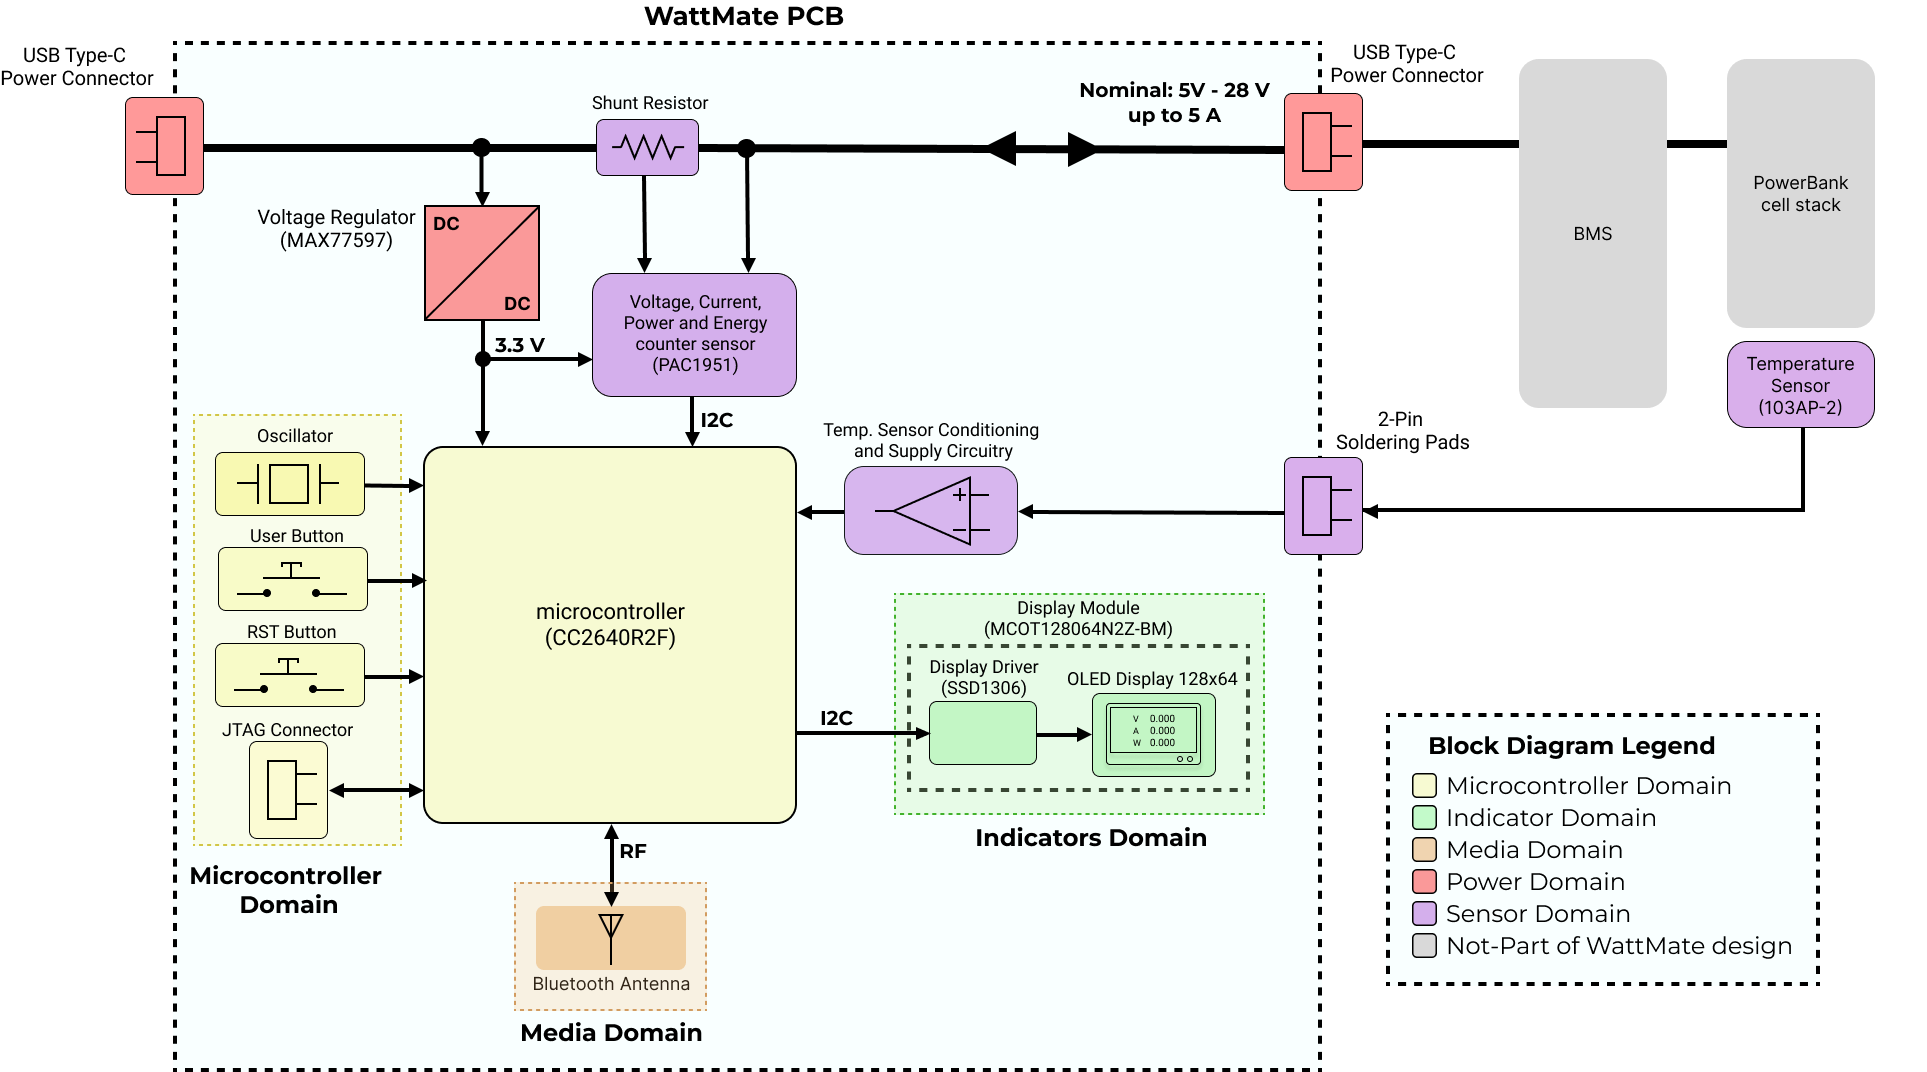
\includegraphics[width=1.0\linewidth]{figures/1_SYS_figures/block_diagram.png}
    \caption{System block diagram showing functional architecture and interconnection between subsystems.}
    \label{fig:block_diagram}
\end{figure}


\subsubsection{Power Connectors and DC Bus}

The main power path, hereafter referred to as the DC bus, represents the primary energy transfer path within the system. It is interrupted by the current sensing element and connects the DC input port to the DC output port. The DC input port is defined as the port always connected to the power bank or battery pack, while the DC output port is defined as the port that, during the discharge phase, is connected to the load. This nomenclature is fixed and is consistently maintained even during the charging phase of the power bank or battery pack.

\subsubsection{Electrical Measurement}

This subsystem performs monitoring of the DC bus electrical quantities, which are then transmitted to the MCU for further analysis and display. In order to save space on the board and keep connection complexity low, measured data are transmitted through a serial communication interface, reducing the number of required signal lines. This subsystem is also responsible for the alert generation, which shall operate according to the safety requirement~\ref{req:over_alert}.

\subsubsection{Temperature Measurement}

A temperature sensing circuit is also included in the prototype. In the current version of WattMate, the sensor can not be directly attached to any battery cells, since the device is implemented as an external inline monitor. However, this functionality was included to validate a sensing approach that could become relevant in future versions of the system, especially in the case of direct integration into the electronics of a battery pack or power bank, as described in Section~\ref{system_objectives}. 

This subsystem performs monitoring of the battery pack temperature, which is then transmitted to the MCU for further analysis and display. In the future integrated system, proper measurement of the battery pack temperature requires the sensor to be placed in direct thermal contact with the cells, which is not feasible if the sensing element is fixed on the main PCB. For this reason, the temperature sensor is connected to the system through wires or metal leads, allowing flexible placement of the sensing element while keeping the main board compact and electrically unchanged.

\subsubsection{RF Communication}

The RF communication subsystem enables wireless data exchange between WattMate and external devices through Bluetooth Low Energy (BLE), providing access to measurement data and system status information. To maintain a compact and cost-effective design the RF interface is integrated directly within the system architecture, avoiding the need for an external antenna. This approach is compatible with the required short-range communication typical of BLE applications.

\subsubsection{User Interface}

The user interface subsystem provides local interaction between the user and the system. Through an integrated display, it presents all measured and computed quantities, as well as system status information and fault or alarm conditions.
As for the other subsytems, data transfer between the MCU and the display is implemented through a serial communication interface, in order to keep connection complexity low.
This subsystem also captures user input through a physical button and forwards it to the MCU for handling display navigation and system control operations.


\subsubsection{MCU}

The MCU represents the central coordination element of the overall system. It is responsible for acquiring data from the sensor and user input subsystems and coordinating their operation to implement the required timing behavior.

The acquired data are processed by the MCU to compute derived quantities such as power, energy, State of Charge (SoC), and State of Health (SoH). These results are made locally available to the user through the display. The MCU also manages the BLE communication, which is implemented with a bidirectional channel, allowing the system to receive commands and data from external devices as well as transmit measurement data and telemetry information.

The MCU also supervises and controls all previously mentioned subsystems to ensure correct system operation while optimizing overall power consumption. This contributes to maximizing battery life by dynamically managing system resources based on operational needs.



\subsubsection{Power Supply}

The power supply subsystem generates and regulates the internal voltage rail required for the operation of all the subsystems. It ensures correct operation under varying input conditions by deriving a stable supply by stepping down the power bank provided voltage.

The power supply is powered from the output connector side of the system in order to achieve accurate estimation of the power bank capacity. In this configuration, during a charging cycle, WattMate measures only the current flowing into the battery pack, excluding the contribution of the system's own consumption. Since the system consumption cannot be easily measured and compensated for, this architectural choice enables accurate capacity estimation without the need for additional sensing circuitry.


%--------------------------------------------------
% Hardware Design
\chapter{Hardware Design}

\section{Component Selection and Sizing}

The hardware architecture of WattMate was developed to satisfy the system requirements defined in Chapter 1 while maintaining compact dimensions, low power consumption, ease of manufacturing, and future expandability.

Component selection was driven primarily by the electrical and functional requirements of the system, with particular attention to measurement accuracy, power efficiency, integration level, package manufacturability, and compatibility with USB Power Delivery operating conditions.

Since the system is intended to operate as an inline measurement device, all selected components were required to minimize their impact on the main power path. This resulted in a design philosophy that prioritizes:
\begin{itemize}
    \item low insertion losses along the DC bus;
    \item reduced internal power consumption;
    \item limited external component count;
    \item support for manual assembly and debugging;
    \item compact board area occupation;
\end{itemize}

Whenever possible, integrated solutions were preferred over discrete implementations in order to reduce PCB complexity, improve reliability, and simplify assembly.

Component packages were selected according to Requirement ~\ref{req:manufacturing-assembly}, prioritizing package sizes compatible with manual soldering and laboratory prototyping while maintaining electrical performance. Passive components were selected with a minimum package size of 0603, except where larger packages were required for power handling, thermal performance, or mechanical robustness.

Particular attention was dedicated to minimizing measurement-induced errors. Components belonging to the sensing chain were selected considering their contribution to the total measurement uncertainty, while power path components were sized to minimize voltage drop and power dissipation.

The following sections describe the rationale behind the selection and sizing of each major hardware subsystem and explain how the adopted solutions satisfy the requirements introduced in Section~\ref{sec:system_requirements}.


%========================================================
% Microcontroller - CC2640R2F
%========================================================
\subsection{Microcontroller - CC2640R2F}

\begin{figure}[H]
    \centering
    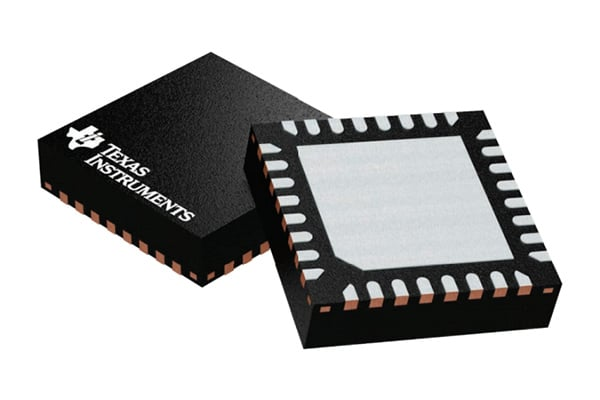
\includegraphics[width=0.5\textwidth]{figures/2_HW_figures/cc2640r2f.jpg}
    \caption{CC2640R2FRHB microcontroller.}
    \label{fig:cc2640r2f}
\end{figure}

According to the requirement ~\ref{req:mcu}, the Texas Instruments CC2640R2F was selected as the main microcontroller for the system. This device belongs to the SimpleLink family and features a 32-bit ARM Cortex-M3 core running at up to 48 MHz, 128 KB of flash memory, and 28 KB of RAM ~\cite{mcu_datasheet}. It also integrates a Bluetooth Low Energy (BLE) radio compliant with Bluetooth 5.1, which enables wireless communication with the mobile application. This MCu comes in three different package options: a 7x7 mm 48-pin VQFN package, a 5x5 mm 32-pin VQFN package, and a 4x4 mm 32-pin VQFN package. Considering the estimated GPIO usage of the system (see Table~\ref{tab:gpio_summary}), both 32-pin variants (including power and auxiliary pins) provide a sufficient number of I/O pins for the current architecture. The CC2640R2FRHB 5x5 mm package version was selected as it also provides a larger footprint compared with the 4x4 mm variant, making it more suitable for manual assembly.

\begin{table}[H]
\centering
\caption{Preliminary estimation on GPIO usage based on System Architecture}
\label{tab:gpio_summary}

\renewcommand{\arraystretch}{1.3}
\renewcommand{\tabularxcolumn}[1]{m{#1}}

\begin{tabularx}{\textwidth}{>{\raggedright\arraybackslash}X>{\centering\arraybackslash}c>{\raggedright\arraybackslash}X}
\toprule
\textbf{Subsystem} & \textbf{GPIO Usage} & \textbf{Interface Notes} \\
\midrule

Electrical Measurement Interface &
2-6 &
Serial interface (UART/I2C/SPI) + alert lines \\

Temperature Measurement &
1 &
Analog sensor connected to ADC pin \\

Display (User Interface) &
2-4 &
Serial interface (UART/I2C/SPI) possibly shared with electrical measurement \\

User Input &
1 &
Physical button with interrupt-capable GPIO \\

RF Communication (BLE) &
2-3 &
Integrated CC2640R2F BLE controller \\

Debug / Programming (JTAG) &
4 &
Standard JTAG interface (TMS, TCK, TDI, TDO, RESET) \\

\midrule
\textbf{Total Estimated GPIO Usage} &
\textbf{12-19 GPIOs} & \\
\bottomrule
\end{tabularx}
\end{table}

To allow proper operation of the MCU, as well as compliance with the system requirements, the following external components have been included within the MCU domain. In addition to the circuitry strictly required for microcontroller operation, this section also includes auxiliary components directly interfaced with the MCU and contributing to system-level functionalities.

\begin{itemize}
    \item \textbf{Reset Circuitry:} A low side push button combined with a \SI{100}{\kilo\ohm} pull-up resistor is connected to the RESET pin of the MCU to ensure it remains in a known state during power-up while also allowing manual reset during development and debugging activities. A \SI{100}{\nano\farad} capacitor is also included to improve reset signal stability, avoiding reset glitches. Since the push button is intended for development purposes, it will not be included in the final product.

    \item \textbf{Quartz Crystals:} A 24 MHz crystal oscillator is included as the main system clock source for the MCU, providing the required frequency stability for full-speed operation, peripheral timing, and communication interfaces.
    
    A dedicated 32.768 kHz crystal oscillator is included as a stable and low-drift reference clock for low-power modes and BLE sleep scheduling, ensuring compliance with the BLE timing requirements. In BLE connected operation, both master and slave devices are required to maintain a sleep clock accuracy within approximately ±500 ppm in order to guarantee correct timing of connection events and to limit the duration of the RX receive window. A less accurate sleep clock would increase the required guard time during reception windows, directly increasing average current consumption and reducing overall power efficiency.

    \item \textbf{Programming Interface:} A 4x2-pins JTAG header is provided for programming and debugging the MCU. This includes connections for TMS, TCK, TDI, TDO, and RESET signals, as well as VDD and GND pins connected according to Table ~\ref{tab:jtag_pinout}.
    
            \begin{table}[H]
                \centering
                \caption{4×2 JTAG Connector Pinout}
                \label{tab:jtag_pinout}

                \renewcommand{\arraystretch}{1.3}

                \begin{tabular}{r|c|c|l}
                    \cline{2-3}

                    GND  & 1 & 2 & TDI \\
                    \cline{2-3}

                    GND  & 3 & 4 & TDO \\
                    \cline{2-3}

                    NRESET  & 5 & 6 & TMSC \\
                    \cline{2-3}

                    VDD  & 7 & 8 & TCKC \\

                    \cline{2-3}

                \end{tabular}
            \end{table}
    \item \textbf{User Input Push Button}
        A low side push button, combined with a \SI{10}{\kilo\ohm} pull-up resistor, is connected to a GPIO pin of the MCU configured as an interrupt input, allowing the system to detect user actions without continuous polling. This button enables user interaction with the device, allowing display activation and the navigation between different screen views. A through-hole (TH) component has been selected beacause, in the final product, this interface represents the primary user interaction element and the TH implementation offers higher mechanical robustness and long-term reliability compared to smaller SMD alternatives. Moreover, during the development and testing phase, the system is operated without a mechanical enclosure, meaning that a standard surface-mounted tactile switch would be less comfortable to use and more exposed to mechanical damage.
    
    \item \textbf{Internal Power Supply Circuitry:}

        The CC2640R2F power architecture is based on three main internal supply domains: VDDS, VDDR, and VDDC. The VDDS rail represents the external supply input to the device and can operate over a wide voltage range. It feeds the internal power management unit, which generates all other required supply rails. The VDDR rail is the main regulated supply domain of the device and can be both generated internally or provided externally. It provides power to the RF subsystem and most internal functional blocks of the microcontroller. The VDDC rail is generated starting from the VDDS rail and is the supply rail that powers the digital logic and core of the MCU as well as the Always ON (AON) domain.   
            
        \begin{figure}[H]
            \centering
            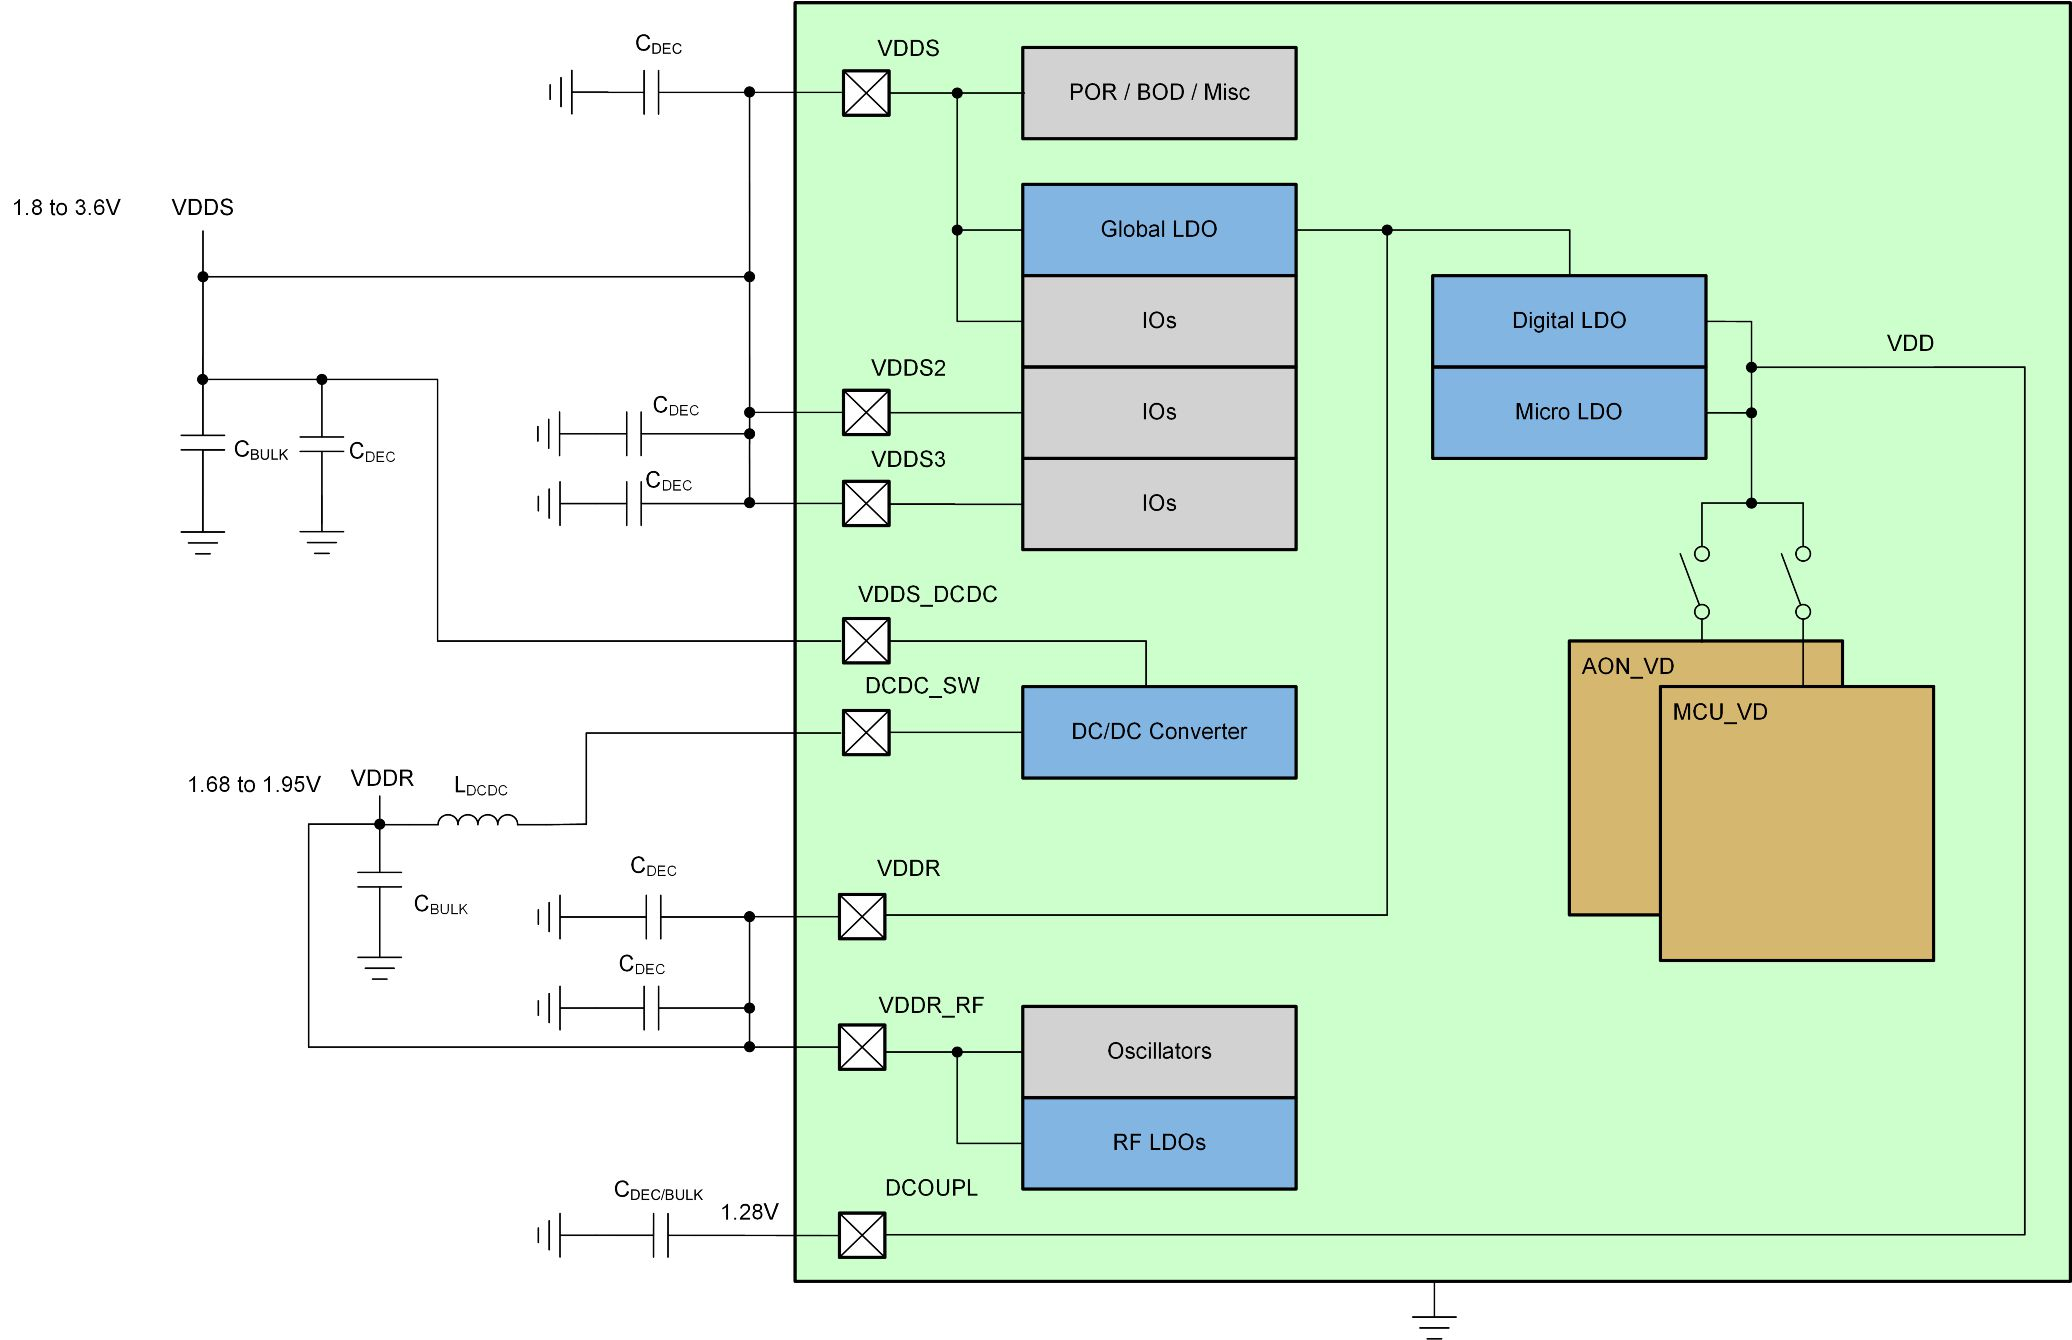
\includegraphics[width=0.85\textwidth]{figures/2_HW_figures/dcdc_converter_mode.jpg}
            \caption{CC2640R2F power architecture and supply configuration highlighting DC-DC converter operation mode.}
            \label{fig:cc2640_power_arch}
        \end{figure}

        The MCU supports three possible power supply configurations for the generation of the VDDR rail:

        \begin{itemize}
            \item \textbf{DC-DC Converter Mode:} The internal switching DC-DC converter generates VDDR from VDDS using an external inductor and capacitor. This mode provides high conversion efficiency and dynamically adapts to load conditions. When operating in this mode the VDDR rail source can be dinamically switched between the internal DC-DC converter and the internal Global LDO regulator, allowing the system to optimize power efficiency across different operating modes.

            \item \textbf{Global LDO Mode:} The VDDR rail is generated using only the internal LDO regulator. This configuration reduces external component count but results in overall higher power dissipation compared to DC-DC operation.

            \item \textbf{External Regulator Mode:} Both VDDS and VDDR are supplied externally, while the internal switching regulator and the Global LDO regulators are disabled. This mode is used when a dedicated external power management solution is available.
        \end{itemize}

        Among these configurations, DC-DC converter mode has been selected for this design.

        The primary reason for this choice is efficiency optimization. Since WattMate is a battery-powered and continuously operating measurement system, minimizing internal power consumption is critical to maximize operational lifetime. DC-DC operation allows the system to maintain higher efficiency across varying load conditions, which is particularly important during active measurement, BLE transmission and data display phases. Although it requires additional external components and careful PCB layout, this trade-off is justified by the substantial improvement in overall power efficiency and battery life.

        In addition, decoupling capacitors were added to ensure stable operation of the power supply rails, consisting of \SI{100}{\nano\farad} capacitors placed on all supply pins and one \SI{10}{\micro\farad} bulk capacitor on each of the main power rails.

\end{itemize}

%========================================================
% RF Antenna - Inverted-F Antenna
%========================================================
\newpage
\subsection{RF Antenna - Inverted-F Antenna}

The antenna selection process was guided by the aim of obtaining a compact solution, compliant with Bluetooth Low Energy (BLE) communication in the 2.4 GHz ISM band as required by \ref{req:ble_tx}. Among the various antenna technologies that still provide compact solutions, PCB-integrated antennas were preferred over chip antennas due to their lower cost and better RF performance, despite the increased occupied area. Based on the analysis of the Ti Antenna Selection Quick Guide~\cite{rf_quick_dn}, there main antenna alternatives were identified among pcb integrated antenna solutions: the Meandered Inverted F Antenna (MIFA), the Inverted F Antenna (IFA) and the Meandered Monopole Antenna. These three solutions were compared in terms of RF performance and occupied area, as summarized in Table~\ref{tab:pcb_antennas}.


\begin{table}[h]
\centering
\renewcommand{\arraystretch}{1.5}
\renewcommand{\tabularxcolumn}[1]{m{#1}}
\setlength{\tabcolsep}{6pt}

\caption{Comparison of different PCB antenna solutions}
\label{tab:pcb_antennas}

\begin{tabularx}{\textwidth}{>{\raggedright\arraybackslash}X>{\centering\arraybackslash}X>{\centering\arraybackslash}X>{\centering\arraybackslash}X}
\hline

\textbf{Antenna Type} &
Meandered Inverted F Antenna (MIFA) &
Inverted F Antenna (IFA) &
Meandered Monopole Antenna \\
\hline

\textbf{Layout Shape} &

\includegraphics[width=0.22\textwidth]{figures/2_HW_figures/mifa_antenna.jpg} &

\includegraphics[width=0.22\textwidth]{figures/2_HW_figures/ifa_antenna.jpg} &
\rule{0pt}{13ex}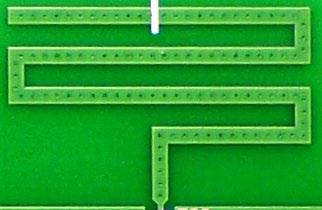
\includegraphics[width=0.18\textwidth]{figures/2_HW_figures/mono_antenna.jpg} \\
\hline

\textbf{Frequency} &
\SI{2.4}{\giga\hertz} &
\SI{2.4}{\giga\hertz} &
\SI{863}{\mega\hertz} + \SI{2.4}{\giga\hertz} (dual band) \\
\hline

\textbf{Typical Efficiency} &
68\% &
80\% &
94\% \\
\hline

\textbf{Bandwidth @ VSWR 2:0} &
\SI{101}{\mega\hertz} &
\SI{280}{\mega\hertz} &
\SI{354}{\mega\hertz} \\
\hline

\textbf{Dimensions (mm)} &
15 x 6 &
26 x 8 &
38 x 25 \\
\hline

\end{tabularx}

\end{table}

The IFA antenna was selected for this design because it provides a good trade-off between efficiency, bandwidth and occupied area. Thanks to its rectangular layout (width: 8mm similar to the MIFA) it can be easily integrated on one side of the PCB, allowing good RF domain separation while having minimal impact over the overall board geometry. Although the MIFA antenna provides a smaller footprint, its reduced efficiency and bandwidth compared to the IFA solution make it less suitable for this application, where reliability and ease of testing and debugging are key requirements. The meandered monopole antenna, while offering the best RF performance, was discarded due to its significantly larger dimensions. In Figure~\ref{fig:ifa_layout} is shown the implemented IFA layout, based on the TI application note~\cite{rf_ifa_ar} whose dimensions are shown in Table~\ref{tab:ifa_dimensions} for complenìteness.

\begin{figure}[H]
    \centering
    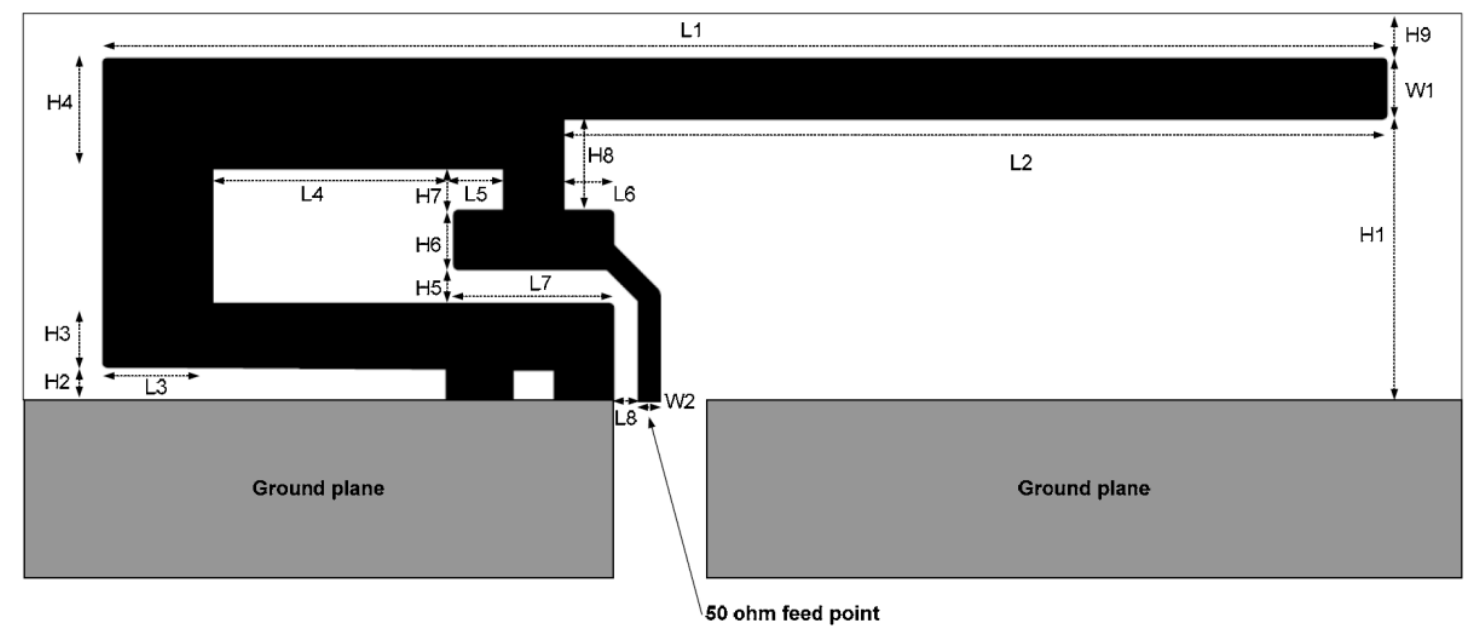
\includegraphics[width=0.95\textwidth]{figures/2_HW_figures/ifa_layout.png}
    \caption{Layout of the implemented Inverted F Antenna (IFA) solution.}
    \label{fig:ifa_layout}
\end{figure}

\begin{table}[h]
    \centering
    \caption{IFA Dimensions}
    \label{tab:ifa_dimensions}
    \renewcommand{\arraystretch}{1.3}

    \begin{tabularx}{\textwidth}{|>{\centering\arraybackslash}X|>{\centering\arraybackslash}X|>{\centering\arraybackslash}X|>{\centering\arraybackslash}X|}
        \hline
        \textbf{Parameter} & \textbf{Value} & \textbf{Parameter} & \textbf{Value} \\
        \hline
        H1 & 5.70 mm & W2 & 0.46 mm \\
        \hline
        H2 & 0.74 mm & L1 & 25.58 mm \\
        \hline
        H3 & 1.29 mm & L2 & 16.40 mm \\
        \hline
        H4 & 2.21 mm & L3 & 2.18 mm \\
        \hline
        H5 & 0.66 mm & L4 & 4.80 mm \\
        \hline
        H6 & 1.21 mm & L5 & 1.00 mm \\
        \hline
        H7 & 0.80 mm & L6 & 1.00 mm \\
        \hline
        H8 & 1.80 mm & L7 & 3.20 mm \\
        \hline
        H9 & 0.61 mm & L8 & 0.45 mm \\
        \hline
        W1 & 1.21 mm &  &  \\
        \hline
    \end{tabularx}
\end{table}

After selecting the appropriate \SI{2.4}{\giga\hertz} antenna solution, the RF front-end design was completed based on the comparison data provided in the application note~\cite{mcu_an}. The CC2640R2F supports four different RF front-end configurations , obtained through different combinations of signaling scheme and biasing options (see Figure~\ref{fig:rf_frontend}). The selected configuration for this design is the single-ended signaling scheme with external biasing. Single-ended signaling is preferred in applications where power consumption is a significant design constraint, while external biasing is used to maintain good sensitivity. The implemented front-end circuit is shown in Figure~\ref{fig:rf_frontend_circuit} and follows the reference design provided by Texas Instruments for single-ended implementation~\cite{rf_ifa_rd}.


\begin{figure}[H]
    \centering
    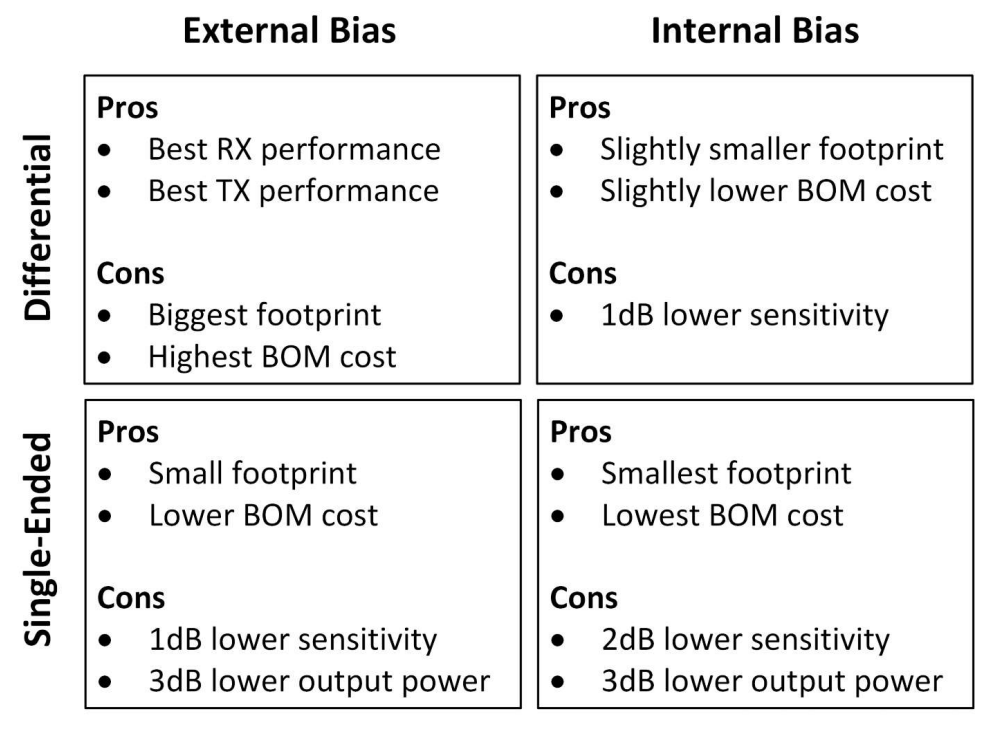
\includegraphics[width=0.7\textwidth]{figures/2_HW_figures/rf_front_end.png}
    \caption{Comparison of CC13xx/CC26xx Front-End Configuration.}
    \label{fig:rf_frontend}
\end{figure}

\begin{figure}[H]
    \centering
    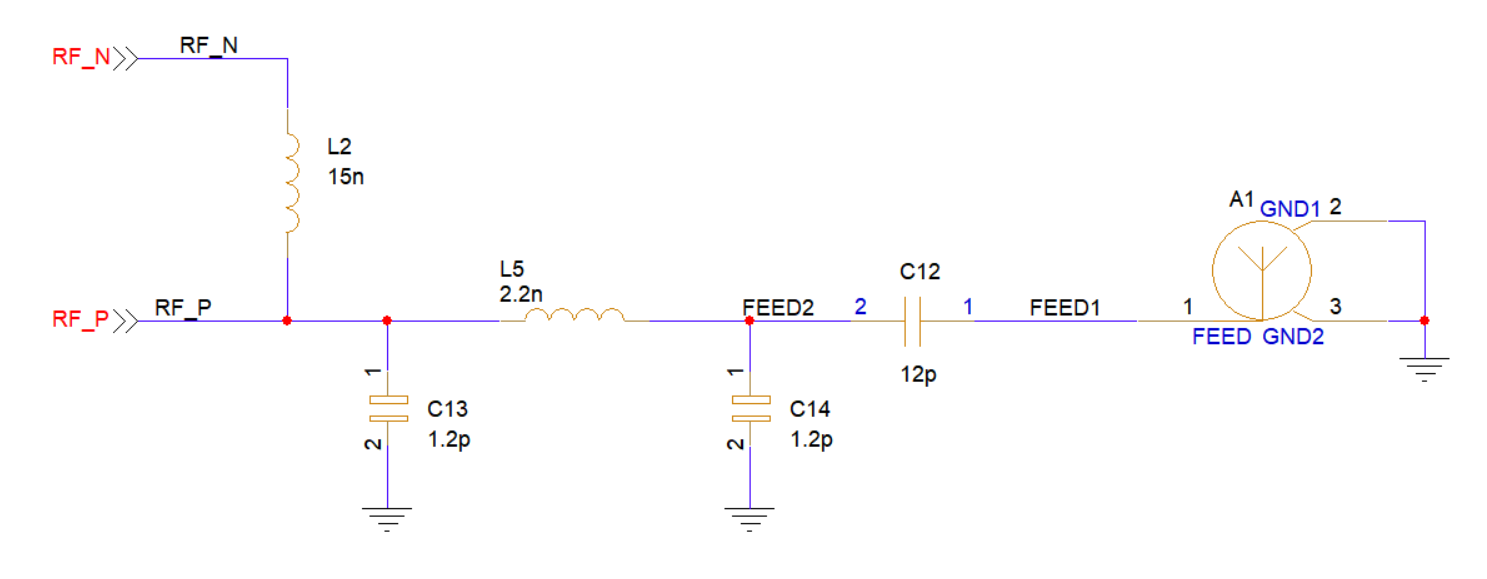
\includegraphics[width=1\textwidth]{figures/2_HW_figures/rf_frontend_circuit.png}
    \caption{Implemented RF Front-End circuit.}
    \label{fig:rf_frontend_circuit}
\end{figure}


%========================================================
% Voltage and Current Sensor - PAC1951
%========================================================
\newpage
\subsection{Voltage and Current Sensor - PAC1951}

\subsubsection{Uncertainty Analysis}
The current measurement sensing architecture is based on a precision shunt resistor $R_S$, where the load current is indirectly obtained from the voltage drop across it. Among the possible sensor technologies, the preferred solution is the use of a dedicate current and voltage measurement IC, which internally integrates the ADC and provide a digital output to the MCU. This approach was selected over discrete implementations based on operational amplifiers and MCU internal ADCs because it allows the MCU to remain in low-power modes during measurement aquisition. For the chosen architecture the nominal current measurement is given by:

\begin{equation}\label{current_meas}
I_S = \frac{V_{S}}{R_S}
\end{equation}

However, the actual measurement is affected by two independent error sources:
\begin{itemize}
    \item \textbf{ADC Measurement Uncertainty:} The internal ADC of the PAC1951 introduces gain error, offset error and integral non-linearity that affect the accuracy of the voltage measurement across the shunt resistor.
    According to the standard ADC error model, the total measurement uncertainty can be expressed as:

    \begin{equation}\label{adc_error}
        \Delta V_{S} = \Delta G \cdot V_{S} + INL \cdot V_{S} + V_{OFF} + \frac{Q}{2}
    \end{equation}

    where:
    \begin{itemize}
        \item $V_{S}$ is the voltage drop across the shunt resistor,
        \item $\Delta G$ is the gain error of the measurement system,
        \item $INL$ is the integral non-linearity of the ADC,
        \item $V_{OFF}$ is the input-referred offset voltage of the ADC,
        \item $Q$ is the quantization step of the ADC
    \end{itemize}
    
    \item \textbf{Shunt Resistor Tolerance:} The shunt resistor $R_S$ has a specified tolerance ($\Delta R_S$) that contributes to the overall measurement uncertainty.

\end{itemize}

Following a first-order uncertainty propagation approach, starting from Eq.~\ref{current_meas}, the total current measurement error can be expressed as:

\begin{equation}
\Delta I_S = \frac{\Delta V_{S} + \Delta R_{S} \cdot I_S}{R_S}
\end{equation}

from which the relative error expression is obtained by substituting Eq.~\ref{adc_error} for $\Delta V_{S}$:

\begin{equation}
\varepsilon_{rel} = \frac{\Delta I_{S}}{I_{S}} =
\Delta G + INL + \Delta R_S +
\frac{V_{OFF} + \frac{Q}{2}}{R_S \cdot I_S}
\end{equation}


The first three terms represent static gain and component-related uncertainties, while the last term introduces a current-dependent contribution that dominates at low current levels. This term explains the steep increase in relative error observed in the low-current region. This formulation was used to compare different current sensing solutions by evaluating their sensitivity to measurement uncertainty over the operating range defined by the requiremnt~\ref{req:measurement-current}.

Similarly to the current measurement, the nominal voltage measurement is given by:
\begin{equation}
V_{BUS} = V_{meas}
\end{equation}

The measurement is affected by the same ADC-related uncertainty sources described for the current channel, namely gain error, integral non-linearity, offset voltage, and quantization error. The total voltage uncertainty can be expressed as:

\begin{equation}\label{adc_v_uncertainty}
\Delta V_{BUS} =
\Delta G \cdot V_{BUS} +
INL \cdot V_{BUS} +
V_{OFF} + \frac{Q}{2}
\end{equation}

Unlike the current measurement, no shunt resistor contribution is present, so the uncertainty is dominated by ADC non-idealities and becomes less dependent on the measured value. This results in a more uniform relative error across the operating range.

\subsubsection{Sensor Selection}
\begin{figure}[H]
    \centering
    
\includegraphics[width=0.35\textwidth]{figures/2_HW_figures/pac1951.png}
    \caption{PAC1951T-1E/4MX sensor.}
    \label{fig:pac1951}
\end{figure}

The PAC1951 was selected as the current and voltage monitoring IC because its characteristics closely match the measurement, power consumption, and system integration requirements defined for WattMate. The most relevant features that motivated this choice are summarized below:

\begin{itemize}

    \item \textbf{Electrical Characteristics:}

    \begin{table}[H]
        \centering
        \renewcommand{\arraystretch}{1.3}
        \caption{Electrical characteristics of the PAC1951 power monitor}
        \label{tab:pac1951_electrical}

        \begin{tabularx}{0.9\textwidth}{|l|X|c|c|c|}
            \hline
            \textbf{Symbol} &
            \textbf{Parameters} &
            \textbf{Typical} &
            \textbf{Maximum} &
            \textbf{Unit} \\
            \hline

            $V_{DD}$ & Supply voltage & 3.3 & 5.5 & \SI{}{\volt} \\
            \hline

            \multirow{2}{*}{$I_{DD,ACTIVE}$} 
            & Active supply current (1024 SPS) & 395 & 535 & \SI{}{\micro\ampere} \\ \cline{2-5}
            & Active supply current (8 SPS) & 12 & 130 & \SI{}{\micro\ampere} \\
            \hline

            $I_{DD,SLEEP}$ & Sleep mode supply current & 5 & - & \SI{}{\micro\ampere} \\
            \hline

        \end{tabularx}
    \end{table}
    The PAC1951 requires a low-voltage supply rail, $V_{DD}$, to power its internal digital logic and I\textsuperscript{2}C interface. The same $V_{DD}$ power rail is also used to supply the analog section of the current and voltage sensing circuitry within the IC.

    \item \textbf{Bus Voltage Measurement Range:}  
    The device supports bus voltage measurements from \SI{0}{\volt} to \SI{32}{\volt}, satisfying the operating voltage requirements up to the \SI{28}{\volt} USB Power Delivery profile defined in Requirements~\ref{req:volt_nominal} and ~\ref{req:volt_rating}.

    \item \textbf{Bidirectional Current Measurement:}  
    The PAC1951 supports bidirectional current sensing through differential shunt voltage measurement with full-scale ranges up to $\pm\SI{100}{\milli\volt}$ that can be programmed dynamically via the control registers to optimize measurement resolution for different load conditions. Combined with a \SI{10}{\milli\ohm} shunt resistor value, this allows accurate measurement of charge and discharge currents up to $\pm\SI{10}{\ampere}$, complying with Requirement~\ref{req:curr_rating}.

    \item \textbf{High Measurement Resolution and Accuracy:}  
    By substituting the worst-case non-ideality parameters reported in the PAC1951 datasheet~\cite{pac1951_datasheet} into the previously derived error model equations, it can be shown that the selected sensor is capable of achieving better than \SI{0.5}{\percent} voltage measurement accuracy and better than \SI{1}{\percent} current measurement accuracy across the specified operating range. This result can be achievd thanks the 16-bit ADCs resolution and the real-time auto-calibration of voltage and current offset error provided by the PC1951.
    Voltage and current error curves were obtained on the entire operating range to verify the compliance with the accuracy requirements, as shown in Figure~\ref{fig:pac1951_error_curves}. Although these values are derived considering worst-case datasheet parameters, the obtained performance still satisfies the requirements defined in~\ref{req:volt_acc} and~\ref{req:curr_acc}. 

    \begin{figure}[H]
        \centering
        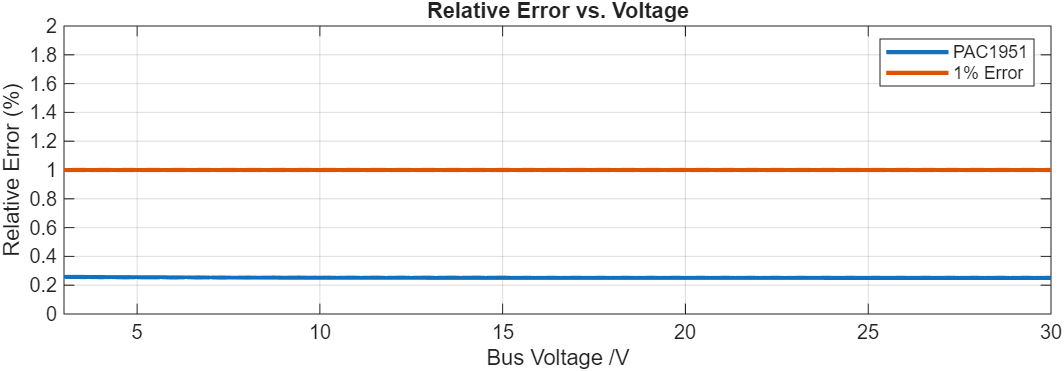
\includegraphics[width=0.8\textwidth]{figures/2_HW_figures/pac_volt_uncertainty.png}
        \vspace{0.5cm}

        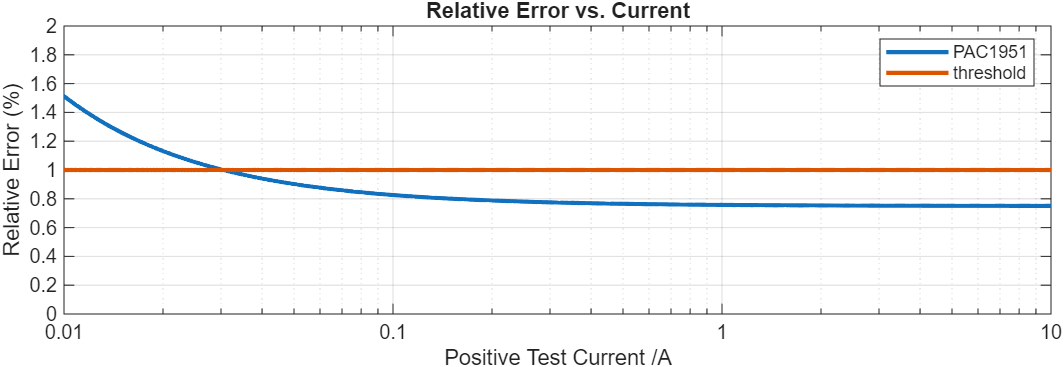
\includegraphics[width=0.8\textwidth]{figures/2_HW_figures/pac_curr_uncertainty.png}
        \caption{Worst case voltage and current measurement error curves for the PAC1951.}
        \label{fig:pac1951_error_curves}
    \end{figure}

    Additionally, given the uncertainty values obtained for voltage and current measurements, the resulting power measurement uncertainty is less than \SI{2}{\percent}, verifying compliance with Requirement~\ref{req:pow_acc}.

    \item \textbf{Integrated Power and Energy Computation:}  
    The PAC1951 internally performs power computation and energy accumulation using dedicated hardware registers. This reduces MCU computational load while supporting the derived quantity calculations required by Requirement~\ref{req:data_proc}.

    \item \textbf{Programmable Sampling Rate:}  
    The device supports programmable sampling rates from \SI{8}{\second\per\second} to \SI{1024}{\second\per\second}, enabling the implementation of different acquisition strategies according to the required measurement update frequency. These capabilities largely exceed the minimum acquisition frequency required by Requirement~\ref{req:perf_sampling}, providing additional design margin.

    \item \textbf{Low-Power System Compatibility:}  
    Since the PAC1951 autonomously performs measurements and accumulation, the MCU can remain in low-power operating modes between acquisitions. This characteristic contributes to compliance with the low-power requirements~\ref{req:pwr_consumption} and~\ref{req:pwr_battery}. Furthermore, when no significant power flow is detected, the PAC1951 can be configured to operate at the minimum sampling rate of \SI{8}{\second^{-1}}, reducing its supply current to \SI{12}{\micro\ampere}, providing additional power saving opportunity.

    \item \textbf{Integrated Fault Detection and ALERT Outputs:}  
    The PAC1951 includes programmable over-voltage, under-voltage, over-current, and overpower detection features, together with two configurable open-drain ALERT outputs. These outputs are connected to MCU interrupt inputs through pull-up resistors, allowing fault conditions to immediately notify the MCU or wake it from low-power modes when an abnormal operating condition is detected.These features simplify the implementation of the protection and notification mechanisms required by Requirements~\ref{req:over_alert} and~\ref{req:under_alert}.

    \item \textbf{Digital I\textsuperscript{2}C Interface:}  
    Communication with the MCU is performed through a standard I\textsuperscript{2}C interface, simplifying PCB routing and reducing the number of required MCU peripherals.

    \item \textbf{Package:}  
    The PAC1951 is available in both 16-pin 3 x 3 mm VQFN and 16-pin 2.2 x 2.2 mm WLCSP packages. The PAC1951T-1E/4MX 3 x 3 mm VQFN package version was selected for this design, as it provides a good balance between compactness and ease of manual assembly, improving manufacturability according to Requirement~\ref{req:assembly}.

\end{itemize}

\begin{figure}[H]
    \centering
    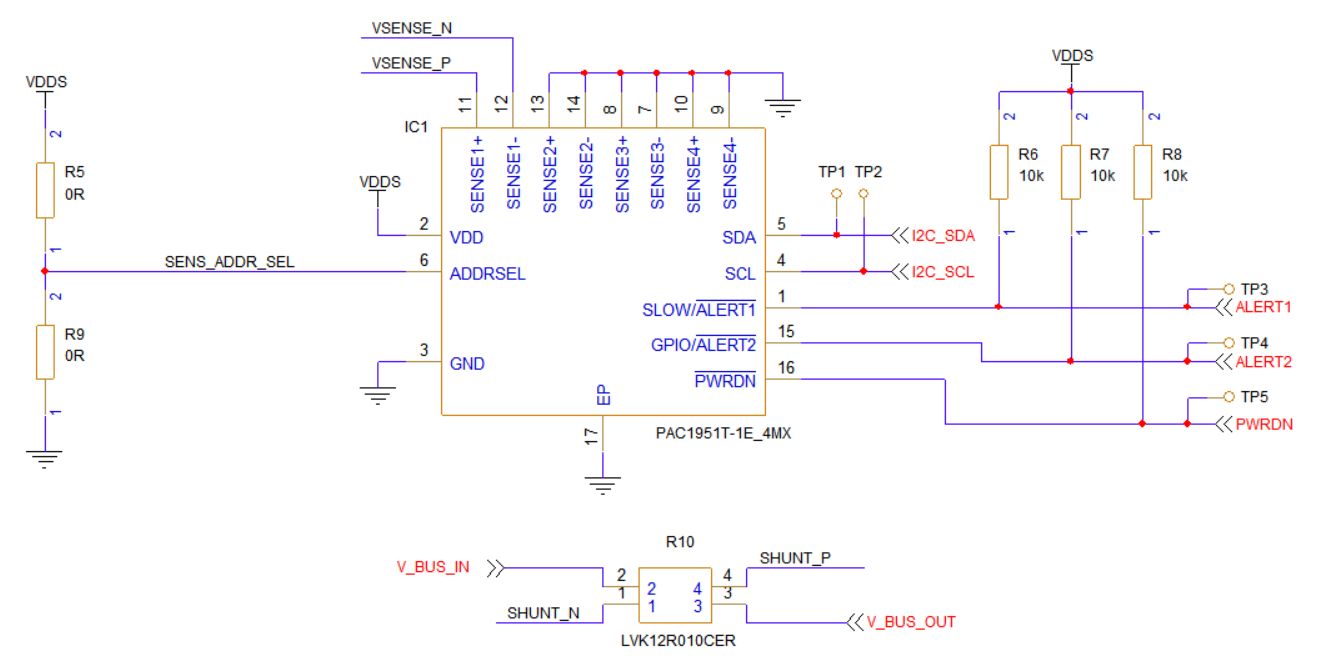
\includegraphics[width=0.95\textwidth]{figures/2_HW_figures/pac_circuit.png}
    \caption{Implemented PAC1951 sensing circuit.}
    \label{fig:pac_circuit}
\end{figure}

To achieve the error performance shown in Figure~\ref{fig:pac1951_error_curves}, a precision shunt resistor is required. In this design, a \SI{10}{\milli\ohm} resistor with \SI{0.25}{\percent} tolerance was selected. The chosen component features dedicated Kelvin sense terminals, which are exclusively used for routing the voltage sensing signals. This configuration improves measurement accuracy by minimizing the impact of parasitic voltage drops along the high-current path and reducing susceptibility to noise.

To further provide noise filtering capability, a differential low-pass input filter was placed between the shunt resistor and the PAC1951 sensing inputs, as shown in Figure~\ref{fig:pac1951_input_filter}. The filter was included as a design margin to allow additional noise mitigation if excessive interference from the environment, switching regulators, or other high-frequency sources is observed during the validation phase. The filter is implemented symmetrically on both sensing lines to preserve differential measurement accuracy and maintain common-mode noise rejection.

Under normal operating conditions, the PAC1951 does not require external input filtering thanks to its internal architecture and real-time offset calibration. However, following discussions with the device vendor, space for a differential input filter was reserved on the PCB to allow future noise mitigation measures, if required, without the need for hardware redesign. 

\begin{figure}[H]
    \centering
    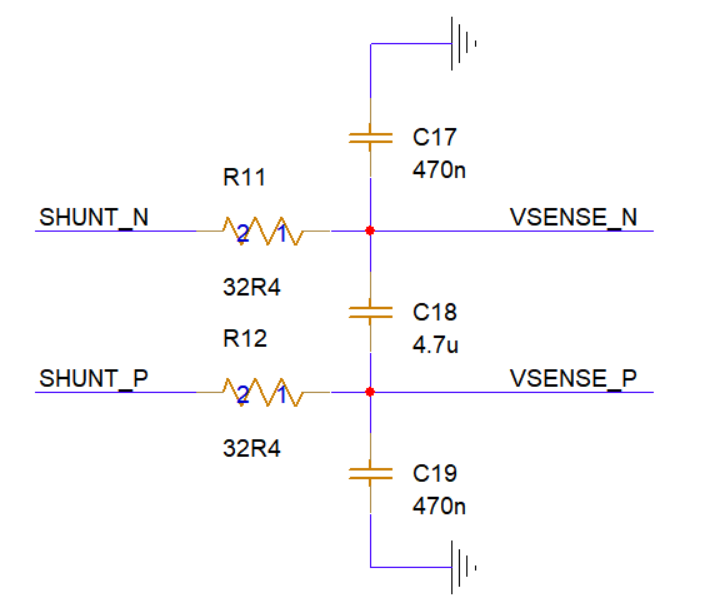
\includegraphics[width=0.55\textwidth]{figures/2_HW_figures/pac1951_input_filter.png}
    \caption{Differential low-pass filter placed between the shunt resistor and the PAC1951 sensing inputs.}
    \label{fig:pac1951_input_filter}
\end{figure}

%========================================================
% Temperature Sensor - NTC Thermistor
%========================================================
\newpage
\subsection{Temperature Sensor - NTC Thermistor}\label{ntc}

The proposed temperature sensing topology is based on a Negative Temperature Coefficient (NTC) thermistor configured in a resistive voltage divider. This sensing approach has been selected as it provides a simple, low-cost and low-power solution for temperature acquisition while maintaining compliance with the system requirements defined in~\ref{req:measurement-temperature}, which are not sufficiently stringent to justify higher-precision and higher-cost sensing solutions. In addition, the use of a thermistor enables a highly flexible placement strategy, which is essential to support the monitoring of the external battery pack, by choosing a leaded package (an approach that would not be easily achievable with integrated IC temperature sensors). The proposed sensing circuit (see Figure~\ref{fig:ntc_divider_circuit}) implement a direct connection with the MCU ADC, avoiding the need for additional digital communication interfaces and simplifying system integration.

\begin{figure}[H]
    \centering
    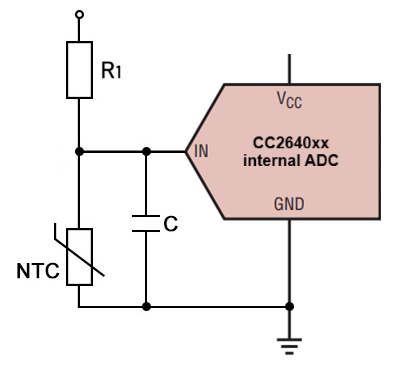
\includegraphics[width=0.4\textwidth]{figures/2_HW_figures/ntc_arch.png}
    \caption{NTC temperature sensing circuit based on a resistive voltage divider.}
    \label{fig:ntc_divider_circuit}
\end{figure}


\subsubsection{Uncertainty Analysis}

\begin{equation}
R_{NTC}(T) = R_0 \, \exp\left[\beta \left(\frac{1}{T} - \frac{1}{T_0}\right)\right]
\end{equation}

where $R_0$ is the nominal resistance at reference temperature $T_0 = \SI{25}{\celsius}$ and $\beta$ is the material constant of the thermistor.
By measuring the output voltage $V_O$ of the resistive divider, the resistance of the thermistor can be expressed as:

\begin{equation}\label{res_div}
R_{NTC} = R_1 \frac{V_O}{V_{DD} - V_O}
\end{equation}

Temperature is then recovered by inverting the Beta equation:

\begin{equation}\label{temp_meas}
T = \left[\frac{1}{T_0} + \frac{1}{\beta}\ln\left(\frac{R_{NTC}}{R_0}\right)\right]^{-1}
\end{equation}


The temperature estimation uncertainty is obtained through first-order propagation applied to the nonlinear transformation. 

\begin{equation}
\label{eq:ntc_total_partial}
\Delta T =
\left|\frac{\partial T}{\partial \beta}\right|\Delta \beta +
\left|\frac{\partial T}{\partial R_0}\right|\Delta R_0 +
\left|\frac{\partial T}{\partial R_{NTC}}\right|\Delta R_{NTC}
\end{equation}


From~\ref{eq:ntc_total_partial}, it is clear that the total uncertainty is decomposed into independent contributions:

\begin{equation}
\Delta T = \Delta T_{\beta} + \Delta T_{R_0} + \Delta T_{R_{NTC}}
\end{equation}

\begin{itemize}

    \item \textbf{Beta parameter uncertainty}

        This term accounts for the sensitivity of the temperature estimation to variations in the thermistor $\beta$ parameter, which introduces a nonlinear error that increases with the logarithmic resistance ratio. By derivating Eq.~\ref{temp_meas} the beta parameter uncertainty term results:

        \begin{equation}
        \Delta T_{\beta} =
        \frac{1}{D^2}
        \left|\frac{\ln\left(\frac{R_{NTC}}{R_0}\right)}{\beta^2}\right|
        \Delta \beta
        \end{equation}

        with

        \begin{equation}
        D = \frac{1}{T_0} + \frac{1}{\beta}\ln\left(\frac{R_{NTC}}{R_0}\right)
        \end{equation}

    
    \item \textbf{Nominal resistance tolerance}
    
    This term represents the effect of the tolerance of the nominal resistance $R_0$ on the temperature estimation accuracy, acting as a constant scaling uncertainty over the full operating range.
        \begin{equation}
        \Delta T_{R_0} =
        \frac{1}{D^2}
        \left|\frac{1}{\beta R_0}\right|
        \Delta R_0
        \end{equation}

\item \textbf{Measured resistance contribution}

The resistance is measured indirectly by knowing the value of the resistor $R_1$ in the voltage divider and by measuring the output voltage of the divider. This approach introduces two additional sources of uncertainty: the error on the measured voltage, due to the ADC, and the tolerance of the resistor $R_1$. By introducing the resistive divider relationship of Eq.~\ref{res_div}, the voltage-related uncertainty propagates to the temperature estimation as follows:

\begin{equation}
\Delta T_{V_O} =
\frac{1}{D^2}
\left|\frac{1}{\beta R_{NTC}}\right|
\left|\frac{R_1 V_{DD}}{(V_{DD} - V_O)^2}\right|
\Delta V_O
\end{equation}

The same reasoning can be applied on the temperature uncertainty term related to the tolerance of the $R_1$ resistor, obtaining:

\begin{equation}
\Delta T_{R_1} =
\frac{1}{D^2}
\left|\frac{1}{\beta R_{NTC}}\right|
\left|\frac{V_O}{V_{DD} - V_O}\right|
\Delta R_1
\end{equation}

\end{itemize}


The total temperature measurement uncertainty is therefore:

\begin{equation}
\Delta T =
\Delta T_{\beta} + \Delta T_{R_0} + \Delta T_{V_O} + \Delta T_{R_1}
\end{equation}


\subsubsection{Sensor Selection}

\begin{figure}[H]
    \centering
    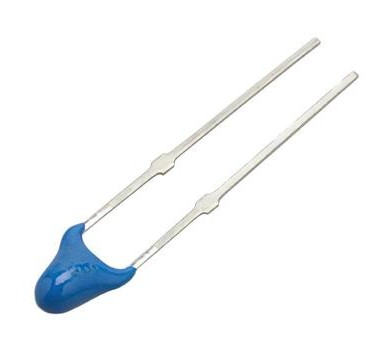
\includegraphics[width=0.35\textwidth]{figures/2_HW_figures/ntc.jpg}
    \caption{103AP-2 NTC sensor.}
    \label{fig:ntc}
\end{figure}

Based on the derived uncertainty model and on the resulting analysis, shown in Figure~\ref{fig:ntc_uncertainty}, the 103AP-2 NTC thermistor was selected in combination with a \SI{5.76}{\kilo\ohm}, \SI{0.1}{\percent} pull-up resistor. The most relevant features that motivated this choice are summarized below:

\begin{itemize}

    \item \textbf{Electrical and uncertainty-related parameters}

        The electrical parameters reported in Table~\ref{tab:ntc_103ap2_params} define both the nominal behavior of the thermistor and its associated modeling uncertainties. In particular, the tolerances on $R_0$ and $\beta$, together with the $R_1$ parameters,  directly affect the temperature estimation accuracy. The chosen combination of components allows compliancy with requirement~\ref{req:temp_acc} (see Figure~\ref{fig:ntc_uncertainty}).

        \begin{table}[H]
            \centering
            \renewcommand{\arraystretch}{1.3}
            \caption{Electrical and uncertainty parameters of the 103AP-2 NTC sencing circuit}
            \label{tab:ntc_103ap2_params}

            \begin{tabular}{|l|l|}
                \hline
                \textbf{Parameter} & \textbf{Value / Description} \\
                \hline
                Nominal resistance $R_0$ & $\SI{10}{\kilo\ohm}$ @ \SI{25}{\celsius} \\
                \hline
                Resistance tolerance & $\pm 0.5\%$ \\
                \hline
                Beta parameter $\beta$ & $\SI{3435}{\kelvin}$ \\
                \hline
                Beta parameter tolerance & $\pm 0.5\%$ \\
                \hline
                Pull-up resistor $R_1$ & $\SI{5.76}{\kilo\ohm}$ \\
                \hline
                Pull-up resistor tolerance & $\pm 0.1\%$ \\
                \hline
            \end{tabular}
        \end{table}

    \item \textbf{Mechanical and environmental characteristics}
        \begin{itemize}
            \item Operating temperature range: \SI{-60}{\celsius} to \SI{150}{\celsius}
            \item Leaded epoxy-coated package enabling flexible placement and off-board sensing
            \item Small sensing element enclosure enabling thermal rise constant of 15 seconds (when suspended in mid-air)
        \end{itemize}


\end{itemize}

\begin{figure}[H]
    \centering
    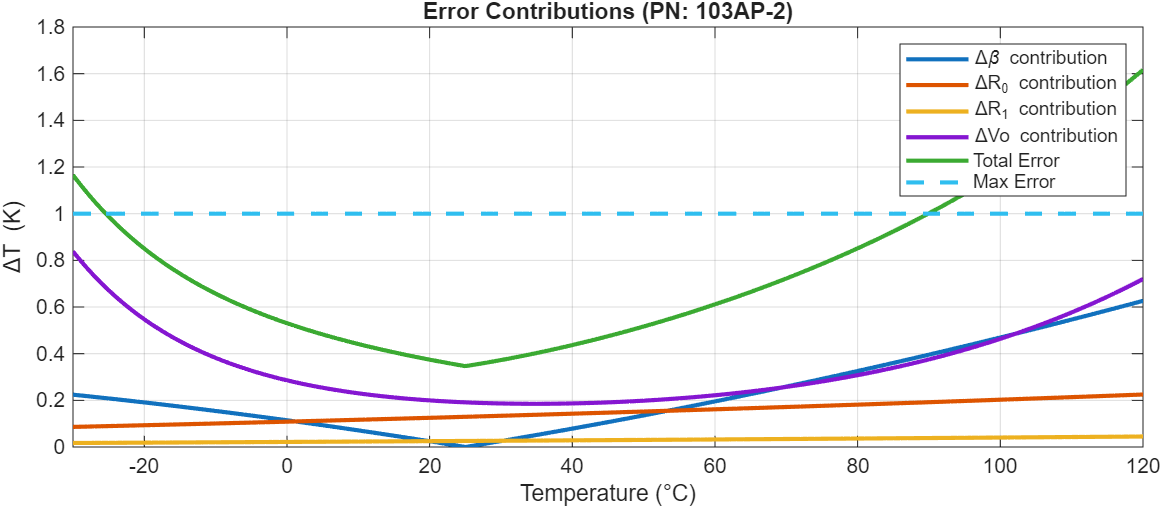
\includegraphics[width=0.9\textwidth]{figures/2_HW_figures/ntc_uncertainty.png}
    \caption{Temperature measurement uncertainty contributions for the selected NTC sensor.}
    \label{fig:ntc_uncertainty}
\end{figure}

Figure~\ref{fig:ntc_circuit} shows the actual implementation of the NTC sensing circuit. In addition to the previously described voltage divider topology, a high-side MOSFET $Q_1$ was introduced to enable the NTC sensing circuit only when temperature acquisition is required, making its leakage current contribution negligible during MCU low-power operation. The gate pull-up resistor $R_{13}$ ensures that the sensing branch is automatically disabled whenever the enable control signal is left floating or interrupted.

At room temperature, the voltage divider dissipates approximately \SI{0.69}{\milli\watt} during ON-state operation. If continuously powered, this static consumption would significantly impact the OFF-state efficiency and reduce the expected battery lifetime, conflicting with the low-power requirements defined in~\ref{req:pwr_battery} and~\ref{req:pwr_consumption}.

\begin{figure}[H]
    \centering
    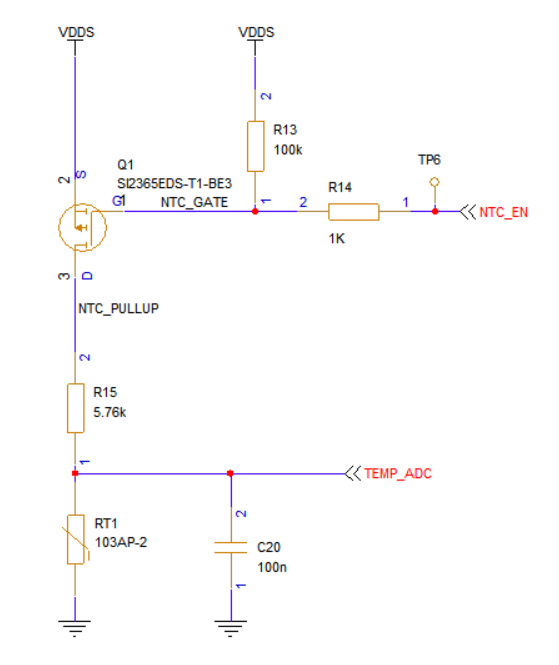
\includegraphics[width=0.55\textwidth]{figures/2_HW_figures/ntc_circuit.png}
    \caption{Implemented NTC sensing circuit with high side switch.}
    \label{fig:ntc_circuit}
\end{figure}


%========================================================
% Display - OLED Display
%========================================================
\newpage
\subsection{Display - OLED Display}

\begin{figure}[htbp]
    \centering
    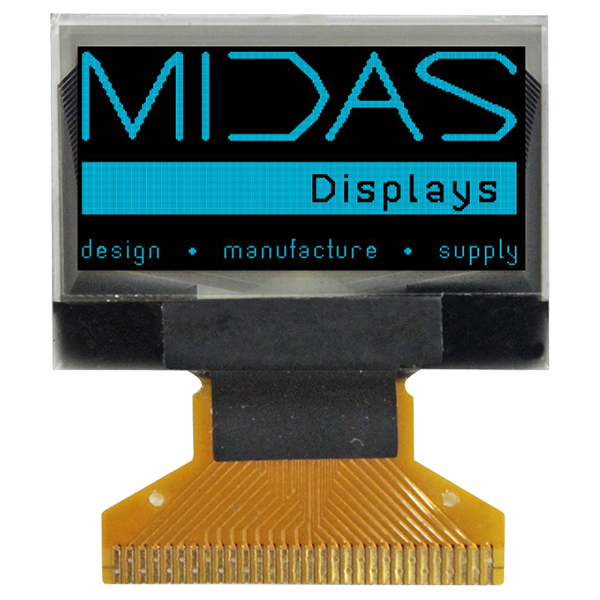
\includegraphics[width=0.4\textwidth]{figures/2_HW_figures/oled_display.png}
    \caption{MCOT128064N2Z-BM OLED display module.}
    \label{fig:oled_display}
\end{figure}

The integration of the OLED display enables the local visualization of measurements, directly satisfying Requirement~\ref{req:ui_display}. The selected display module is the MCOT128064N2Z-BM, a monochrome OLED display featuring a 0.96-inch active area and a resolution of 128 x 64 pixels. The most relevant features and implementation details that motivated this choice are summarized below:

\begin{itemize}

    \item \textbf{Integrated Controller}
    
    The display is based on the widely adopted SSD1306 display controller, which is directly embedded inside the module. This driver integrates both logic and power functionalities, reducing the need for external components and minimizing the overall footprint on the PCB.

    \item \textbf{Electrical Characteristics:}
    
    \begin{table}[H]
        \centering
        \renewcommand{\arraystretch}{1.3}
        \caption{Electrical characteristics of the MCOT128064N2Z-BM display module}
        \label{tab:oled_electrical}

        \begin{tabularx}{0.9\textwidth}{|l|X|c|c|c|}
            \hline
            \textbf{Symbol} &
            \textbf{Parameters} &
            \textbf{Typical} &
            \textbf{Maximum} &
            \textbf{Unit} \\
            \hline

            $V_{DD}$ & Logic supply voltage & 3.3 & 4.0 & \SI{}{\volt} \\
            \hline

            $I_{DD}$ & Normal operation, full display ON & 42 & 127 & \SI{}{\micro\ampere} \\
            \hline

            $I_{DD,SLEEP}$ & Display OFF & - & 10 & \SI{}{\micro\ampere} \\
            \hline

            $V_{CC}$ & Segment supply voltage generated by charge pump & 7.5 & - & \SI{}{\volt} \\
            \hline

            $I_{CC}$ & Normal operation, 50\% display ON & 25.6 & 32 & \SI{}{\milli\ampere} \\
            \hline

        \end{tabularx}
    \end{table}
    The SSD1306 controller requires a low-voltage supply rail, $V_{DD}$, to power its internal digital logic. In addition, the OLED panel requires a higher driving voltage, $V_{CC}$, to supply the display segments. Since the voltage required to drive the OLED pixels is significantly higher than the logic supply voltage, the controller internally generates $V_{CC}$ from the input supply through an integrated charge pump. This is implemented by connecting external \SI{1}{\micro\farad} flying capacitors across the C1P/C1N and C2P/C2N pins, allowing the controller to generate $V_{CC}$ directly from the supply voltage ($V_{DD}$).

    \item \textbf{Serial Interface:} 
    
    To minimize the number of required GPIO pins and simplify PCB routing, the display is configured for I\textsuperscript{2}C communication by connecting the interface configuration pins to the logic levels specified by the SSD1306 controller datasheet.

    \item \textbf{OLED Technology:} 
    
    Unlike traditional LCDs that require a constant power-drawing backlight, the OLED panel consumes power only for its active (lit) pixels. This significantly improves energy efficiency during ON-State operation, supporting Requirement~\ref{req:pwr_consumption}. Moreover, the absence of a backlighting system allows the display to be thinner compared to alternative technologies. Additionally, the OLED panel provides a high contrast ratio and a wide viewing angle to ensure excellent readability.

    \item \textbf{Hardware Contrast Calibration:} 
    
    The panel's brightness and maximum segment current ($I_{SEG}$) are hardware-calibrated via an internal reference current ($I_{REF}$). To achieve the recommended segment current of \SI{100}{\micro\ampere} at the maximum software contrast setting of 255, a precision external pull-down resistor is connected between the $I_{REF}$ pin and analog ground ($V_{SS}$). This maintains the reference current at exactly \SI{12.5}{\micro\ampere}.

    \item \textbf{Mechanical Mounting:} Thanks to the flexible cable, the display can be mounted on the opposite side of the PCB with respect to the connector location by folding the flex cable around the board edge. This approach minimizes the effective PCB footprint, as only the SMD connector occupies board space, while the display module itself is positioned outside the populated side of the PCB.

\end{itemize}



\begin{figure}[htbp]
    \centering
    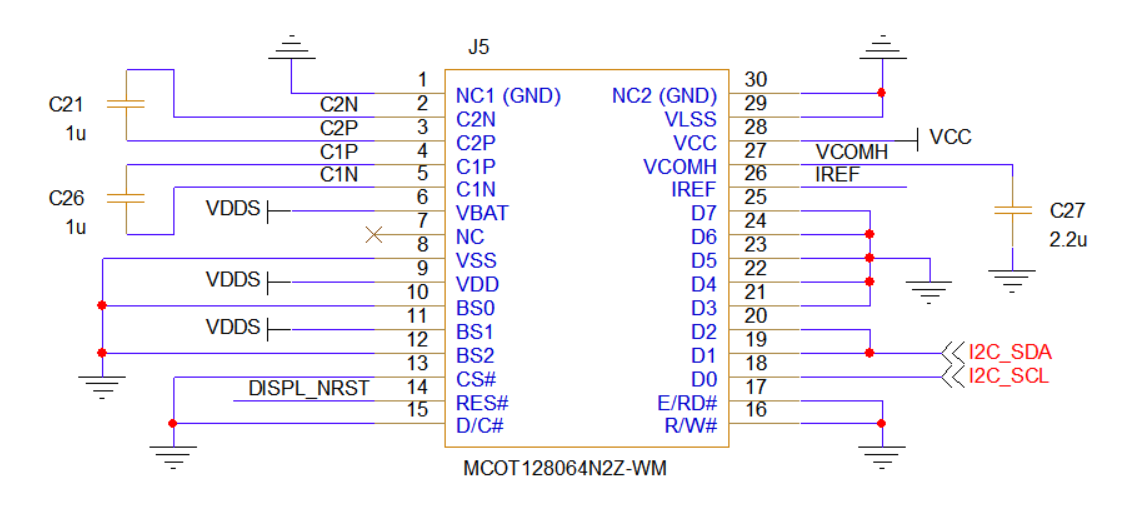
\includegraphics[width=0.9\textwidth]{figures/2_HW_figures/oled_circuit.png}
    \caption{Implemented OLED display circuit.}
    \label{fig:oled_schematic}
\end{figure}

%========================================================
% Power Supply - MAX77597
%========================================================
\newpage
\subsection{Power Supply - MAX77597}\label{sec:schematic_max77597}

\begin{figure}[H]
    \centering
    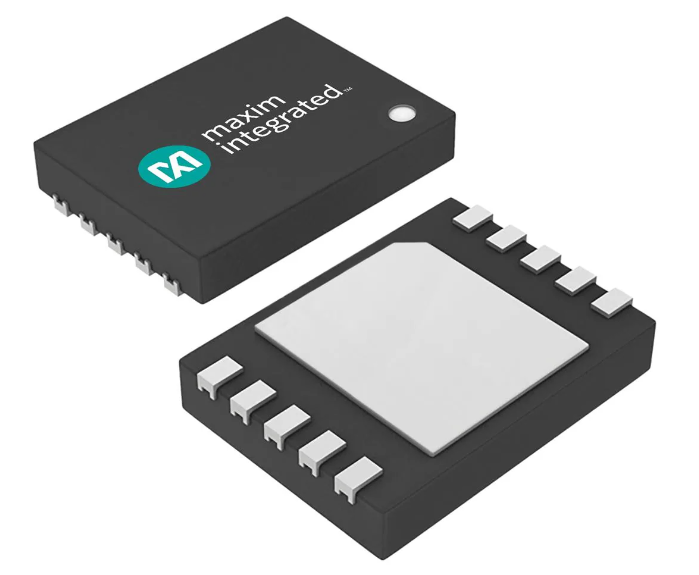
\includegraphics[width=0.4\textwidth]{figures/2_HW_figures/max77597.png}
    \caption{MAX77597ETBB+T synchronous buck converter controller.}
    \label{fig:dcdc}
\end{figure}

As shown in Table~\ref{tab:voltage_summary}, all the circuit subsystems were chosen to be powered by a stable \SI{3.3}{\volt} voltage rail. This rail must be derived directly from the power bus, which can range from \SI{5}{\volt} to \SI{28}{\volt} with a \SI{+5}{\percent} tolerance (up to \SI{29.4}{\volt}) as defined in Requirements~\ref{req:volt_nominal} and~\ref{req:volt_rating}. To fulfill this, the MAX77597 synchronous step-down converter was selected. The most relevant features that motivated this choice are summarized below:

\begin{itemize}

    \item \textbf{Electrical Characteristics:}

    \begin{table}[H]
        \centering
        \renewcommand{\arraystretch}{1.3}
        \caption{Electrical characteristics of the MAX77597 step-down converter}
        \label{tab:max77597_electrical}

        \begin{tabularx}{0.9\textwidth}{|l|X|c|c|c|}
            \hline
            \textbf{Symbol} &
            \textbf{Parameters} &
            \textbf{Typical} &
            \textbf{Maximum} &
            \textbf{Unit} \\
            \hline

            $V_{SUP}$ & Input operating supply voltage & - & 36 & \SI{}{\volt} \\
            \hline
            
            $I_{OUT}$ & Maximum continuous load current & 300 & - & \SI{}{\milli\ampere} \\
            \hline

            $I_{SUP}$ & No-load supply current ($V_{OUT} = \SI{3.3}{\volt}$) & 1.1 & 3.0 & \SI{}{\micro\ampere} \\
            \hline

            $I_{SHDN}$ & Shutdown supply current ($V_{EN} = \SI{0}{\volt}$) & 0.75 & 3.0 & \SI{}{\micro\ampere} \\
            \hline

            $f_{SW}$ & Internal PWM switching frequency & 1.7 & 1.82 & \SI{}{\mega\hertz} \\
            \hline

        \end{tabularx}
    \end{table}

    \item \textbf{Wide Input Voltage Range:} 
    The device operates over a wide input voltage range from \SI{3.5}{\volt} to \SI{36}{\volt}. This provides a robust safety margin above the maximum expected \SI{29.4}{\volt} input, satisfying the over-voltage survival constraints of the USB Power Delivery profiles up to \SI{140}{\watt}.

    \item \textbf{Ultra-Low Quiescent Current:} 
    The regulator consumes only \SI{1.1}{\micro\ampere} (typical) of quiescent current at no load, and drops to \SI{0.75}{\micro\ampere} during shutdown. This ultra-low power consumption is critical for meeting the OFF-State battery life requirement of at least 1 year (~\ref{req:pwr_battery}).

    \item \textbf{High Efficiency Operation:} 

    The internal synchronous rectification eliminates the need for an external schottky diode, improving overall internal efficiency and minimizing thermal dissipation (~\ref{req:power-consumption}). Furthermore, to optimize power consumption during light-load conditions (MCU on low-power states), the device is configured to use a skip PWM mode instead of Forced-PWM (FPWM). In skip-mode operation, the converter's switching frequency is load dependent until the output load reaches the skip threshold. At higher load current the FPWM is enabled, keeping the switching frequency constant and allowing the converter to delivery up to \SI{300}{\milli\ampere} of continuous load current during full ON-state operation. The skip operating mode drastically minimizes switching losses and reduces the operating quiescent current to just \SI{1.1}{\micro\ampere}. This dynamic efficiency is critical for achieving the extended OFF-State battery life required by ~\ref{req:pwr_battery}.

    \begin{figure}[htbp]
        \centering
        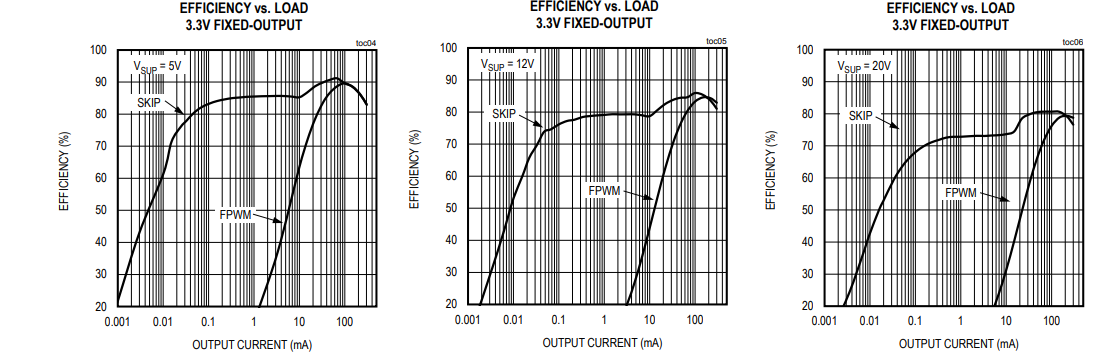
\includegraphics[width=\textwidth]{figures/2_HW_figures/dcdc_efficiency.png}
        \caption{Converter efficiency versus load current at input voltages of \SI{5}{\volt}, \SI{12}{\volt}, and \SI{20}{\volt}, demonstrating performance in both FPWM and skip modes.}
        \label{fig:max77597_efficiency}
    \end{figure}
    

\end{itemize}

\begin{table}[htbp]
    \centering
    \renewcommand{\arraystretch}{1.3}
    \caption{Summary of required voltage rails across PCB subsystems}
    \label{tab:voltage_summary}

    \begin{tabularx}{\textwidth}{|>{\centering\arraybackslash}m{2.5cm}|>{\centering\arraybackslash}m{2cm}|X|X|}
        \hline
        \textbf{Subsystem} &
        \textbf{Voltage} &
        \textbf{Supplied Components} &
        \textbf{Power Source} \\
        \hline

        \textbf{Input Bus}\newline($V_{IN}$) & 
        up to \SI{29.4}{\volt} & 
        DC/DC input,\newline PAC1951 bus ($V_{BUS}$) & 
        External USB Type-C Power Delivery source \\
        \hline

        \textbf{System Logic}\newline($V_{DDS}$) & 
        \SI{3.3}{\volt} & 
        MCU ($V_{DDS}$),\newline PAC1951 ($V_{DD}$),\newline OLED Logic ($V_{DD}$) & 
        DC/DC Converter \\
        \hline

        \textbf{OLED Display}\newline($V_{CC}$) & 
        \SI{7.5}{\volt} & 
        OLED display & 
        SSD1306 internal charge pump \\
        \hline

        \textbf{MCU Internal}\newline($V_{DDR}$) & 
        \SI{1.8}{\volt} & 
        MCU internal RF and Oscillator section& 
        MCU internal DC/DC converter \\
        \hline

        \textbf{MCU Core}\newline($V_{DDC}$) & 
        \SI{1.28}{\volt} & 
        MCU internal digital core & 
        MCU internal Digital LDOs \\
        \hline
        
    \end{tabularx}
\end{table}

The external passive components for the buck converter were sized mathematically following the manufacturer's design guidelines to ensure stability and low noise.

The required inductance ($L$) was calculated to balance the inductor peak-to-peak AC current against the physical size of the component. The value is selected based on the input voltage ($V_{SUP}$), the switching frequency ($f_{SW}$), the expected typical load current ($I_{OUT}$), and a target Inductor Current Ripple Ratio ($LIR$, typically set to $0.3$):

$$L = \frac{V_{OUT} \cdot (V_{SUP} - V_{OUT})}{V_{SUP} \cdot f_{SW} \cdot I_{OUT} \cdot LIR}$$

The output capacitor ($C_{OUT}$) was sized to maintain the output voltage ripple ($V_{RIPPLE(P-P)}$) within the strict limits required by the MCU and ADCs. When utilizing capacitors where the Equivalent Series Resistance ($ESR$) dominates the ripple, the required maximum ESR is calculated as follows:

$$V_{RIPPLE(P-P)} = ESR \cdot I_{LOAD(MAX)} \cdot LIR$$

Finally, the input filter capacitor ($C_{IN}$) was selected to handle the maximum root-mean-square (RMS) ripple current ($I_{RMS}$) drawn by the switching action of the internal MOSFETs. The RMS current requirement reaches its peak when the input voltage is exactly twice the output voltage:

$$I_{RMS} = I_{LOAD(MAX)} \cdot \frac{\sqrt{V_{OUT} \cdot (V_{SUP} - V_{OUT})}}{V_{SUP}}$$

The final implemented circuit is shown in Figure~\ref{fig:max77597_schematic}, where the selected component values are also reported.

An important note must be made regarding the system's ground connections. Proper grounding is critical for the stable, jitter-free operation of the MAX77597 step-down converter. To manage the distinct electrical characteristics within the IC, the device separates its ground into two discrete pins: Analog Ground (AGND) and Power Ground (PGND). The separation of grounds is required to prevent high-frequency switching noise from corrupting the sensitive analog control loops:
\begin{itemize}
    \item \textbf{PGND (Power Ground):} This pin serves as the high-current return path for the internal power MOSFETs and external power components (such as the input capacitor, $C_{IN}$, and output capacitor, $C_{OUT}$). The rapid switching action of the converter generates large current transients (high $di/dt$), which inevitably induce voltage spikes and noise across the power ground plane.
    \item \textbf{AGND (Analog Ground):} This pin acts as the clean, quiet reference ground for the internal analog circuitry, including the \SI{5}{\volt} BIAS regulator, error amplifiers, and feedback comparators. If noisy PGND currents were allowed to flow through the AGND path, it would introduce significant jitter, degrade voltage regulation accuracy, and potentially cause erratic switching behavior.
\end{itemize}


\begin{figure}[htbp]
    \centering
    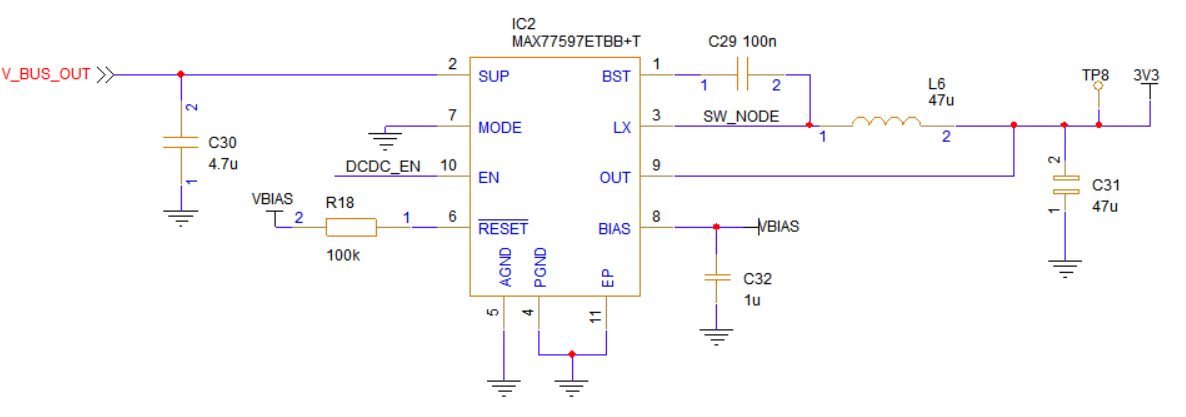
\includegraphics[width=\textwidth]{figures/2_HW_figures/max77597_circuit.png}
    \caption{Schematic diagram of the MAX77597 step-down converter subsystem.}
    \label{fig:max77597_schematic}
\end{figure}

%========================================================
% Connectors - USB Type-C
%========================================================
\newpage
\subsection{Connectors - USB Type-C}

\begin{figure}[H]
    \centering
    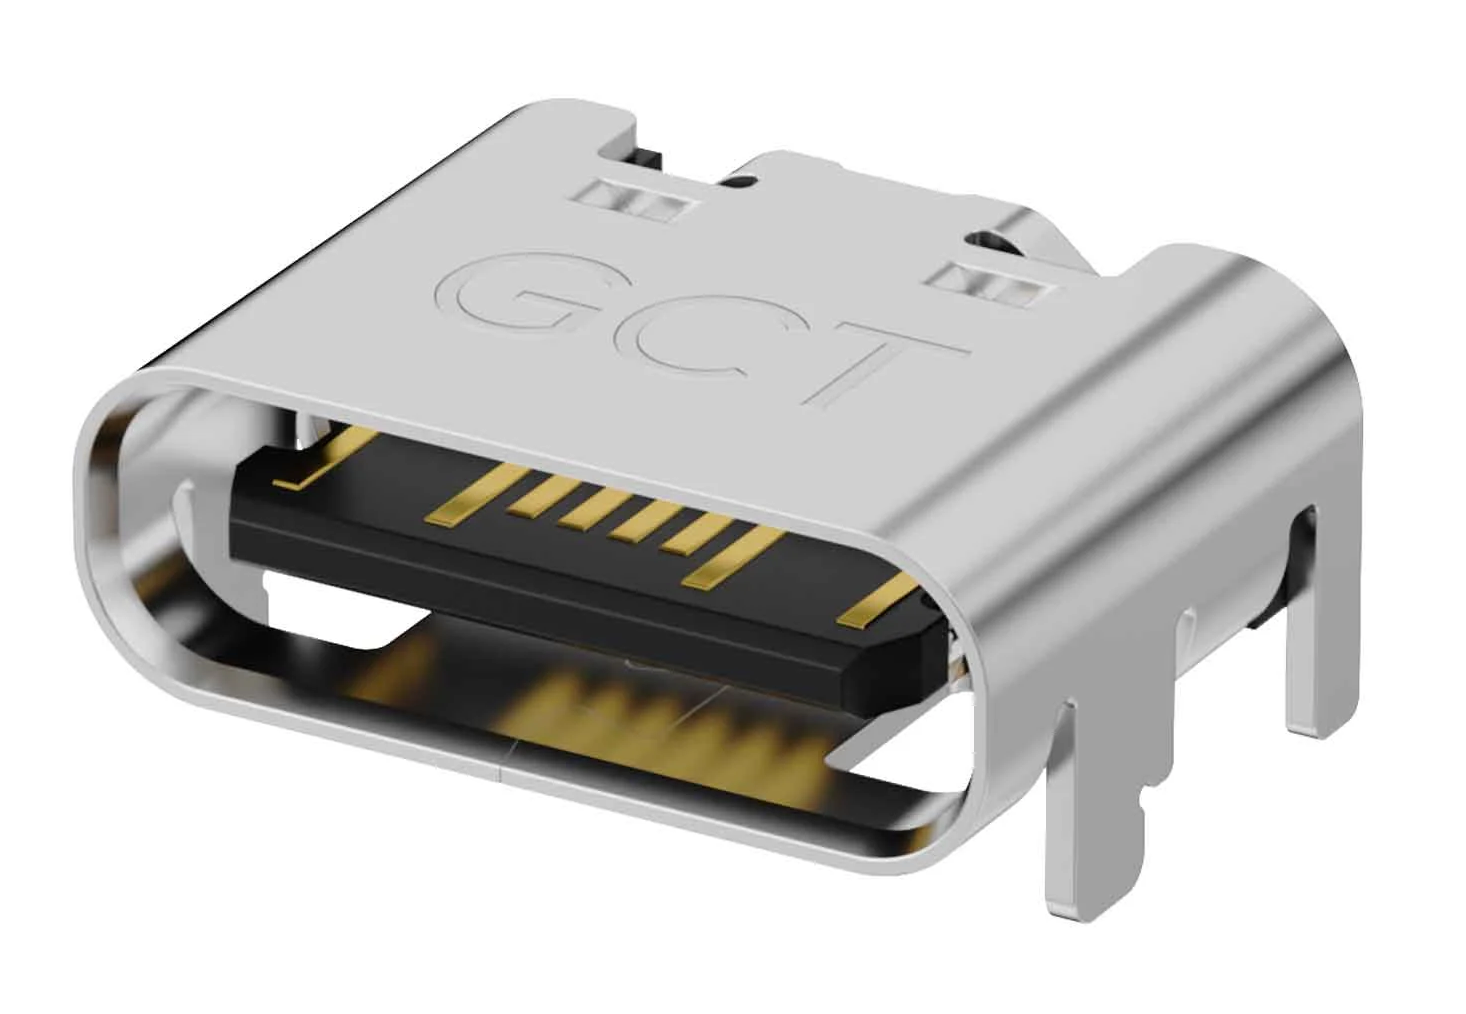
\includegraphics[width=0.4\textwidth]{figures/2_HW_figures/usb.png}
    \caption{USB Type C 16 pin receptacle, SMT horizontal top mount.}
    \label{fig:usb}
\end{figure}

\subsubsection{Component Selection and Requirements Addressed}
The system must operate inline between a power source and a load without interrupting power delivery, while safely handling the full USB Power Delivery 3.1 profile up to \SI{28}{\volt} and \SI{5}{\ampere} (Requirements~\ref{req:volt_table},~\ref{req:curr_rating}, and~\ref{req:inline_op}). To fulfill these physical interface requirements, the GCT USB4215 USB Type-C receptacle was selected for both the input and output ports of the analyzer. The most relevant features that motivated this choice are summarized below:

\begin{itemize}

    \item \textbf{Electrical and Mechanical Characteristics:}

    \begin{table}[H]
        \centering
        \renewcommand{\arraystretch}{1.3}
        \caption{Electrical and mechanical characteristics of the GCT USB4215 receptacle}
        \label{tab:usb4215_characteristics}

        \begin{tabularx}{0.9\textwidth}{|l|X|c|c|c|}
            \hline
            \textbf{Symbol} &
            \textbf{Parameters} &
            \textbf{Typical} &
            \textbf{Maximum} &
            \textbf{Unit} \\
            \hline

            $V_{RATING}$ & Maximum DC voltage rating & - & 48 & \SI{}{\volt} \\
            \hline
            
            $I_{VBUS}$ & Collective current rating for VBUS pins & - & 5.0 & \SI{}{\ampere} \\
            \hline

            $I_{GND}$ & Collective current rating for GND pins & - & 6.25 & \SI{}{\ampere} \\
            \hline

            $R_{CONTACT}$ & Initial contact resistance & - & 40 & \SI{}{\milli\ohm} \\
            \hline
            
            $Cycles$ & Mating durability & 20000 & - & Cycles \\
            \hline

        \end{tabularx}
    \end{table}

    \item \textbf{Extended Power Ratings:} 
    The USB4215 connector is rated for a maximum voltage of \SI{48}{\volt} DC and a collective VBUS current of \SI{5.0}{\ampere}, enabling it to handle up to \SI{240}{\watt} of power. This provides a substantial safety margin for the system's \SI{140}{\watt} target, fully complying with the power delivery requirements (Requirements~\ref{req:volt_table},~\ref{req:curr_rating}, and~\ref{req:pow_rating}).

    \item \textbf{Optimized 16-Pin Configuration:} 
    The receptacle utilizes a 16-pin layout that omits the high-speed SuperSpeed (Tx/Rx) data pins, which are unnecessary for this power analysis application. However, it retains the essential VBUS, GND and Configuration Channel (CC1/CC2) pins. This ensures that the system does not interfere with the USB Power Delivery negotiation process between the source and the sink (Requirement~\ref{req:inline_pd}) while significantly simplifying the PCB layout and assembly.

    \item \textbf{High Durability and Low Contact Resistance:} 
    The connector features an initial contact resistance of just \SI{40}{\milli\ohm} (maximum) and is rated for \num{20000} mating cycles. This minimizes parasitic voltage drops across the inline connection—crucial for maintaining measurement accuracy (Requirement~\ref{req:volt_acc})—and ensures long-term mechanical reliability.

    

\end{itemize}

\subsubsection{Component Sizing and Implementation Details}
To satisfy the inline operation requirement (Requirement~\ref{req:inline_op}), two USB4215 connectors are mounted on opposite edges of the PCB. One acts as the power input from the source, and the other acts as the output to the load. The Configuration Channel (CC1, CC2) are passed straight through between the two connectors. This passive passthrough guarantees that the system remains transparent to the USB Power Delivery negotiation process.

While connectors do not require mathematical sizing in the same way as active power converters, evaluating the worst-case power dissipation ($P_{LOSS}$) across the connector is critical to ensure thermal stability under continuous heavy loads. The maximum power dissipated by the connector's contact resistance ($R_{CONTACT}$) at the absolute maximum rated current ($I_{MAX}$) is calculated as:

$$P_{LOSS} = I_{MAX}^2 \cdot R_{CONTACT}$$

For the maximum targeted operating current of \SI{5}{\ampere} and the worst-case initial contact resistance of \SI{40}{\milli\ohm}, the expected power loss is:

$$P_{LOSS} = (\SI{5}{\ampere})^2 \cdot \SI{40}{\milli\ohm} = \SI{1.0}{\watt}$$

This \SI{1.0}{\watt} worst-case dissipation per connector highlights the necessity of the large VBUS and GND copper pours on the PCB, that will be further analyzed in the layout consideration Section~\ref{layout_considerations}. These pours act not only as high-current carrying traces but also as essential thermal heatsinks to wick heat away from the connector's Surface Mount Technology (SMT) pads, ensuring the system operates safely within the targeted temperature bounds.


%========================================================
%========================================================
%========================================================
% PCB Design
%========================================================
%========================================================
%========================================================
\newpage
\section{PCB Design}


\subsection{Component Placement Strategy}\label{component_placement_strategy}
The physical floorplanning of the PCB was dictated by the need to isolate distinct electrical domains, specifically separating high current power delivery, sensitive analog measurements, noisy switching regulators, and high frequency RF transmission. 

The two USB Type-C connectors are placed on opposite edges of the board to facilitate an intuitive inline connection between the power source and the load. The high-current power path, including the series shunt resistor, the PAC1951 measurement IC, and the MAX77597 step-down converter, is strictly confined to the upper half of the board. 

The CC2640R2F microcontroller (MCU) and the remaining subsystems, such as the user-interface buttons and OLED display connector, are centrally located. This centralized placement is strategic since it minimizes trace lengths and prevents signals from requiring long, convoluted paths with excessive via transitions, thereby improving overall signal integrity. Furthermore, this positions the display and buttons optimally for ergonomic user access and visibility.

Finally, the \SI{2.4}{\giga\hertz} RF matching network and PCB antenna are positioned at the very bottom edge of the PCB. This strict physical separation maximizes the distance from the DC/DC converter in the upper half, effectively preventing high-frequency switching noise from coupling into the sensitive RF front-end.

\begin{figure}[H]
    \centering

    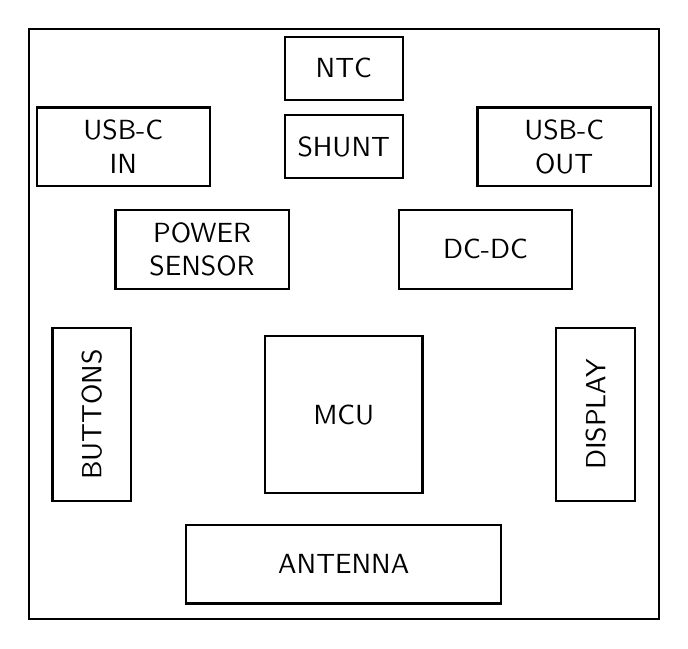
\begin{tikzpicture}[
        block/.style={draw, thick, minimum width=2.2cm, minimum height=1cm, align=center},
        smallblock/.style={draw, thick, minimum width=1.5cm, minimum height=0.8cm, align=center},
        wideblock/.style={draw, thick, minimum width=4cm, minimum height=1cm, align=center},
        box/.style={draw, thick, minimum width=2cm, minimum height=2cm, align=center},
        line/.style={thick}
    ]

    % Outer boundary
    \draw[thick] (0,0) rectangle (8,7.5);

    % USB-C IN / OUT
    \node[block] (usbin) at (1.2,6) {USB-C\\IN};
    \node[block] (usbout) at (6.8,6) {USB-C\\OUT};

    % NTC
    \node[smallblock] (ntc) at (4,7) {NTC};

    % SHUNT
    \node[smallblock] (shunt) at (4,6) {SHUNT};

    % DC-DC
    \node[block] (dcdc) at (5.8,4.7) {DC-DC};

    % Power sensor
    \node[block] (ps) at (2.2,4.7) {POWER\\SENSOR};

    % MCU
    \node[box] (mcu) at (4,2.6) {MCU};

    % Buttons
    \node[block, rotate=90] (buttons) at (0.8,2.6) {BUTTONS};

    % Display
    \node[block, rotate=90] (display) at (7.2,2.6) {DISPLAY};

    % Antenna
    \node[wideblock] (antenna) at (4,0.7) {ANTENNA};


    \end{tikzpicture}

    \caption{System architecture floorplanning.}
    \label{fig:block_diagram}
\end{figure}


%========================================================
% Layer Stackup and Impedance Control
%========================================================
\subsection{Layer Stackup and Impedance Control}\label{stackup}

\subsubsection{Layer Stackup Architecture}
To satisfy the conflicting demands of high-current power delivery (\textbf{Requirement~\ref{req:curr_rating}}), sensitive analog measurements, and high-frequency RF transmission (\textbf{Requirement~\ref{req:ble_tx}}), a 4-layer Printed Circuit Board (PCB) architecture was selected. The chosen stackup (see Figure) provides the necessary routing flexibility and solid reference planes required for a mixed-signal design. 

The layer assignment was strategically defined as follows:
\begin{itemize}
    \item \textbf{Top Layer (L1 - Signal / RF / GND):} Houses all surface-mount components, the \SI{2.4}{\giga\hertz} PCB antenna, the critical RF matching network, and the massive copper polygon pours required to carry the \SI{5}{\ampere} VBUS current. The remaining available area is filled with a ground pour, stitched to the internal and bottom ground planes through a dense via network, providing a low-impedance return path, improved EMI performance, enhanced RF behavior, and effective current return routing.
    \item \textbf{Internal Layer 1 (L2 - Solid GND):} Dedicated entirely as a continuous, unbroken Ground plane. This serves three critical functions: it provides a low impedance return path for all signals, acts as the immediate dielectric reference plane for the RF impedance control, and serves as a massive thermal heat spreader for the power connectors and shunt resistor.
    \item \textbf{Internal Layer 2 (L3 - Power):} Dedicated to the distribution of the internally generated \SI{3.3}{\volt} logic supply ($V_{DDS}$). Using a solid power plane minimizes the power distribution network impedance, improves supply voltage stability, and provides additional inter-plane capacitance with the adjacent ground layer, contributing to high-frequency decoupling.
    \item \textbf{Bottom Layer (L4 - Signal / GND):} Used for secondary signal routing and placement of test points required for debugging and validation activities. The remaining area is filled with a ground pour, stitched to the top and internal ground layers through vias.    

\end{itemize}

\begin{figure}[H]
    \centering
    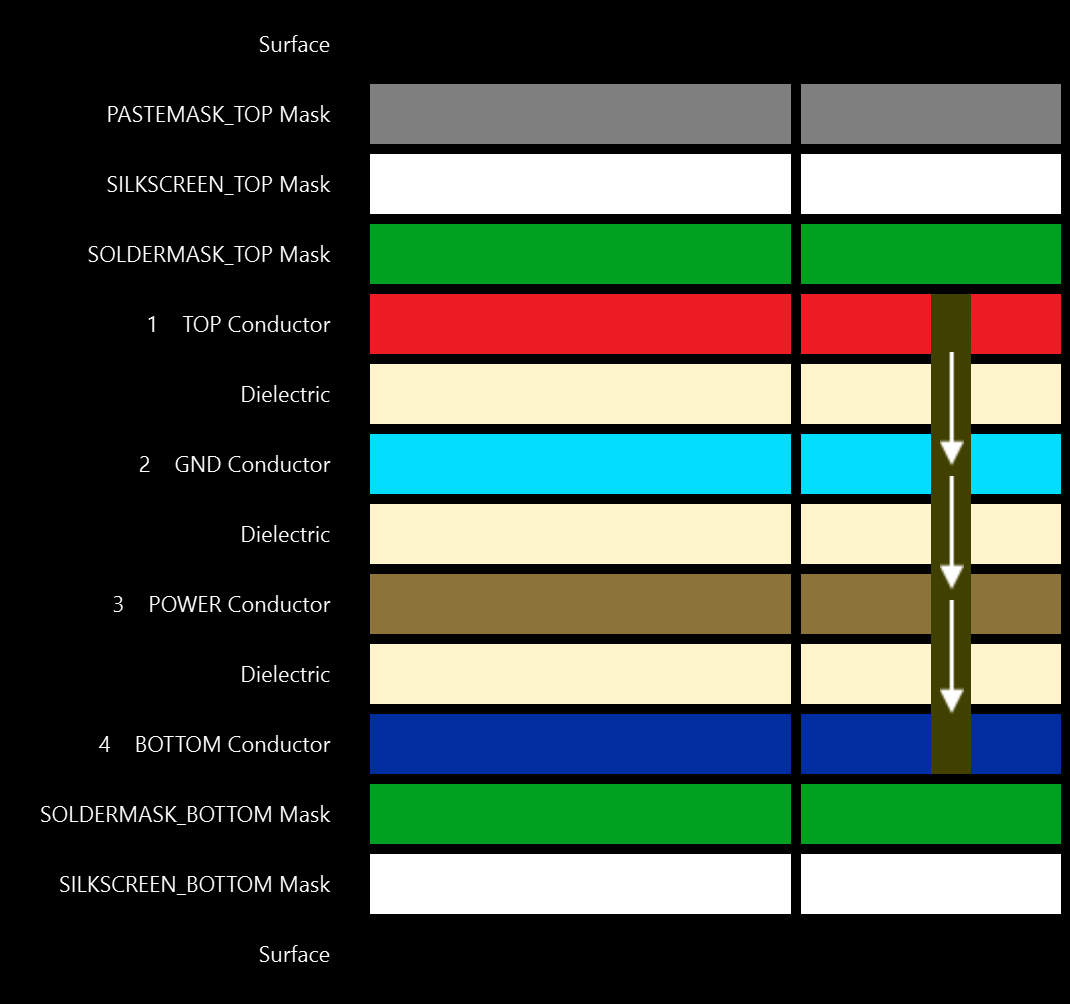
\includegraphics[width=0.75\textwidth]{figures/2_HW_figures/stack_pcb.png}
    \caption{Cross-sectional profile of the 4-layer PCB stackup.}
    \label{fig:layer_stackup}
\end{figure}


\subsubsection{RF Impedance Control}\label{rf_impedance_control}
To ensure reliable BLE communication, the RF front-end must minimize signal reflection and maximize power transfer to the antenna. This dictates that the trace connecting the CC2640R2F microcontroller to the antenna feed point must be designed as a controlled \SI{50}{\ohm} transmission line.

In the PCB manufacturer website, the JLC04161H-7628 stack-up shown in Figure~\ref{fig:impedance_calc} was selected as a cost effective solution that still provides adequate electrical performance for the target application. Given the 4-layer stackup, the RF transmission line is modeled as a surface coplanar waveguide with ground (CPWG). The characteristic impedance $Z_0$ is a function of the trace width $W$, the clearance gap to the adjacent top layer ground pour $S$, the copper thickness $T$, the dielectric constant of the FR-4 substrate ($\epsilon_r \approx 4.5$), and the dielectric height to the reference ground plane $H$. By utilizing the manufacturer's specific tool based on the selected JLC04161H-7628 stackup parameters, the trace width was mathematically calculated to hit the target \SI{50}{\ohm} impedance.

\begin{figure}[H]
    \centering
    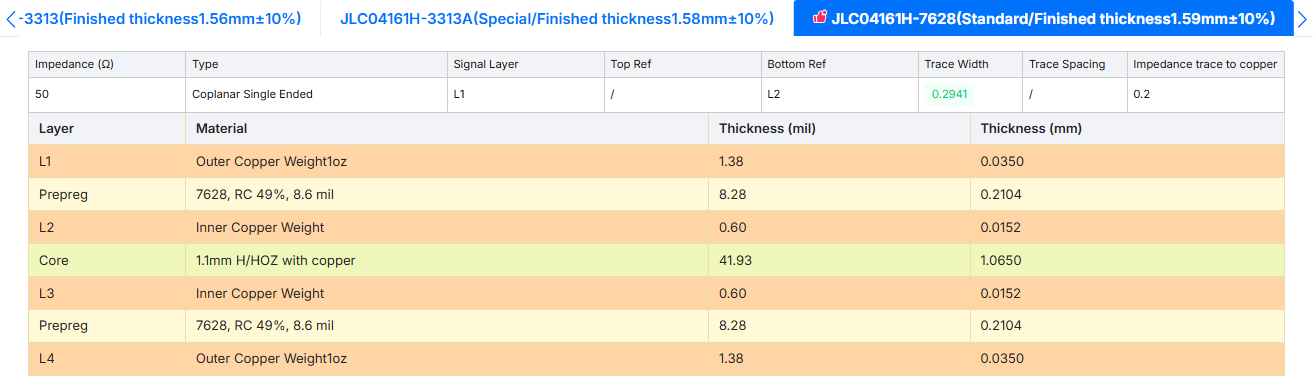
\includegraphics[width=\textwidth]{figures/2_HW_figures/stack_jlc.png}
    \caption{PCB manufacturer's impedance calculation tool used to determine the required \SI{50}{\ohm} trace width, based on the selected layer stack-up and material properties.}
    \label{fig:impedance_calc}
\end{figure}

%========================================================
% Constraints and Design Rules Considerations
%========================================================

\subsection{Constraints and Design Rules Considerations}
The Design Rule Check (DRC) parameters and layout constraints were defined to balance optimal electrical performance with cost effective, standard manufacturing capabilities (\textbf{Requirement~\ref{req:packages}}).

\subsubsection{Trace Width Sizing}
Conductor widths were categorically assigned based on their specific electrical domain:
\begin{itemize}
    \item \textbf{Power Lines (VBUS, GND, \SI{3.3}{\volt}):} As will be later discussed in section~\ref{vbus_size}, the \SI{5}{\ampere} VBUS and GND nets were routed massive multi-layer polygon pours rather than standard traces to prevent thermal overload and excessive voltage drop. The \SI{3.3}{\volt} logic supply, delivering up to \SI{300}{\milli\ampere} from the MAX77597, was routed with minimum trace widths of \SI{0.25}{\milli\meter} to ensure low DC resistance while still allowing routing access through densely populated areas of the PCB.
    \item \textbf{RF Lines (\SI{2.4}{\giga\hertz}):} The antenna feed trace width was derived from controlled impedance requirements rather than an arbitrary design choice. Based on the analysis in Section~\ref{rf_impedance_control}, a CPWG structure was used to achieve a \SI{50}{\ohm} characteristic impedance, resulting in a calculated trace width of \SI{0.294}{\milli\meter}.
    \item \textbf{Analog Lines:} The analog signal traces are routed with minimum width to reduce the exposed copper surface that can couple to external noise sources. Moreover, these traces carry negligible current, making narrow routing fully appropriate from an electrical perspective. Differential traces connecting the PAC1951 to the shunt resistor and the NTC sensing network follow this routing strategy. These traces are implemented with a width of \SI{0.15}{\milli\meter}, also ensuring compliance with the lowest-cost manufacturing class supported by the PCB manufacturer.
    \item \textbf{Normal/Digital Lines (GPIO, $I^2C$):} Similarly to analog traces, GPIO digital lines are low-current signals. In this case, narrow routing is particularly useful to allow escape routing from the dense MCU pin area and to maintain routability in high-density regions of the PCB layout, without compromising signal integrity. These traces are implemented with a width of \SI{0.15}{\milli\meter}.
\end{itemize}

\subsubsection{Via Dimensions}

To reduce manufacturing costs and simplify the PCB fabrication process, only Plated Through-Hole (PTH) vias were used throughout the design. This approach avoids the additional complexity and cost associated with blind, buried, or microvias while remaining fully compatible with the routing density and performance requirements of the system.

The standard via size was set to a \SI{0.3}{\milli\meter} drill diameter with a \SI{0.5}{\milli\meter} annular ring pad. This \SI{0.3}{\milli\meter} via hole size incurs no additional drilling charges, while remaining small enough to be densely arranged in via arrays for thermal dissipation. It also fits within the exposed thermal pads of the ICs without causing solder drainage issues during reflow, ensuring both manufacturability and reliable thermal/electrical performance.

\subsubsection{Component Spacing}
Clearance constraints were dictated by assembly reliability (Requirement~\ref{req:assembly}):
\begin{itemize}
    \item \textbf{Passive to Passive Clearance:} Minimum spacing of \SI{0.5}{\milli\meter} was defined to ensure reliable manual soldering and avoid solder bridging, while still allowing high component density in compact regions of the PCB.
    
    \item \textbf{IC to Passive Clearance:} Increased spacing of \SI{1.5}{\milli\meter} was adopted around integrated circuits to facilitate probe access, improve thermal relief during rework, and reduce the risk of accidental solder bridging in densely routed areas.
    
    Figure~\ref{fig:ic_clearance} shows a representative section of the PCB layout illustrating the implemented IC-to-passive spacing.

    \begin{figure}[H]
        \centering
        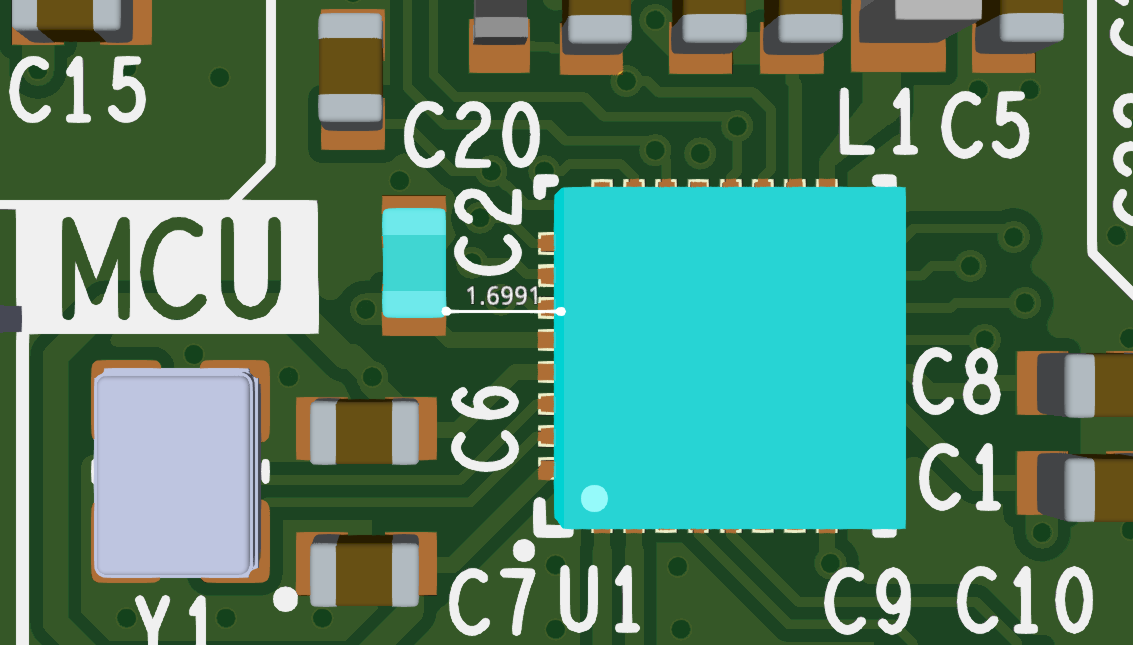
\includegraphics[width=0.7\textwidth]{figures/2_HW_figures/component_clearance.png}
        \caption{Detail of IC to passive clearance measurement on the PCB layout.}
        \label{fig:ic_clearance}
    \end{figure}

\end{itemize}


\subsection{Routing and Layout Considerations}\label{layout_considerations}

    \subsubsection{High-Current Power Path (VBUS)}\label{vbus_size}
        The primary challenge in the power path layout was routing the \SI{5}{\ampere}, \SI{28}{\volt} (up to \SI{140}{\watt}) USB Power Delivery bus between the input and output connectors without exceeding thermal limits or inducing significant voltage drops, which could compromise measurement accuracy (\textbf{Requirement~\ref{req:volt_acc}}). Standard trace routing is insufficient for this current density. 

        To determine the appropriate copper sizing, the Saturn PCB Toolkit was utilized to model the conductor properties, as illustrated in Figure~\ref{fig:saturn_pcb_calc}. Calculations based on a standard \SI{1}{oz/ft^2} (\SI{35}{\micro\meter}) base copper weight demonstrated that a trace width of \SI{4.6}{\milli\meter} carrying \SI{5}{\ampere} yields a safe temperature rise of \SI{20}{\degreeCelsius} (reaching \SI{45}{\degreeCelsius} at a \SI{25}{\degreeCelsius} ambient). Additionally, the predicted voltage drop across this conductor is approximately \SI{16.3}{\milli\volt}.

        To implement this safely and provide additional thermal and electrical margin, \SI{2.8}{\milli\meter} wide copper polygon pours were used to connect the VBUS pins of the USB-C receptacles (see Figure~\ref{fig:main_bus_layout}). By extending these polygons on both the top and bottom layers, the effective cross section exceeds the minimum required width of \SI{4.6}{\milli\meter} when considering parallel conduction paths across multiple layers. To further improve thermal dissipation and current sharing, the same pours are replicated on the internal copper layers and stitched together using dense via arrays. This multi-layer interconnection strategy reduces the overall DC resistance, distributes current more uniformly across the stack-up, and improves heat spreading throughout the PCB structure. The connection of the GND pins is implemented using the same strategy, by exploiting the existing ground planes on layers L1, L2, and L4.

        \begin{figure}[H]
            \centering
            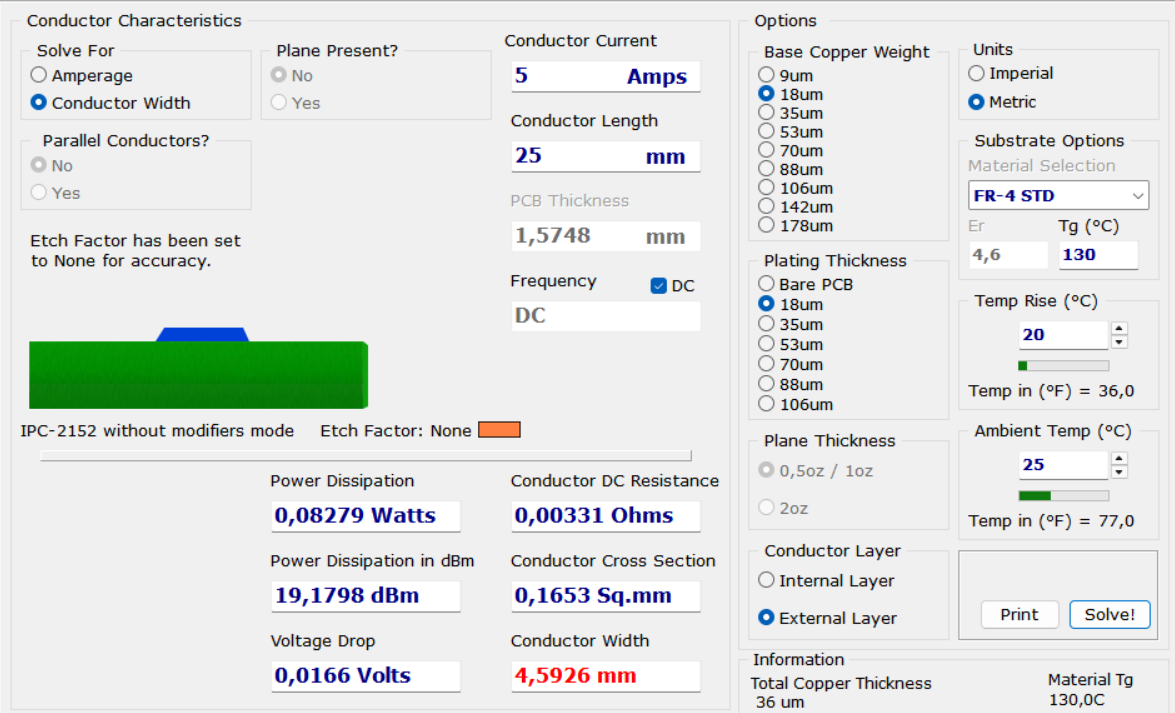
\includegraphics[width=0.9\textwidth]{figures/2_HW_figures/pcb_toolkit.png}
            \caption{Conductor properties calculation using the Saturn PCB Toolkit used to verify trace width.}
            \label{fig:saturn_pcb_calc}
        \end{figure}

        \begin{figure}[H]
            \centering
            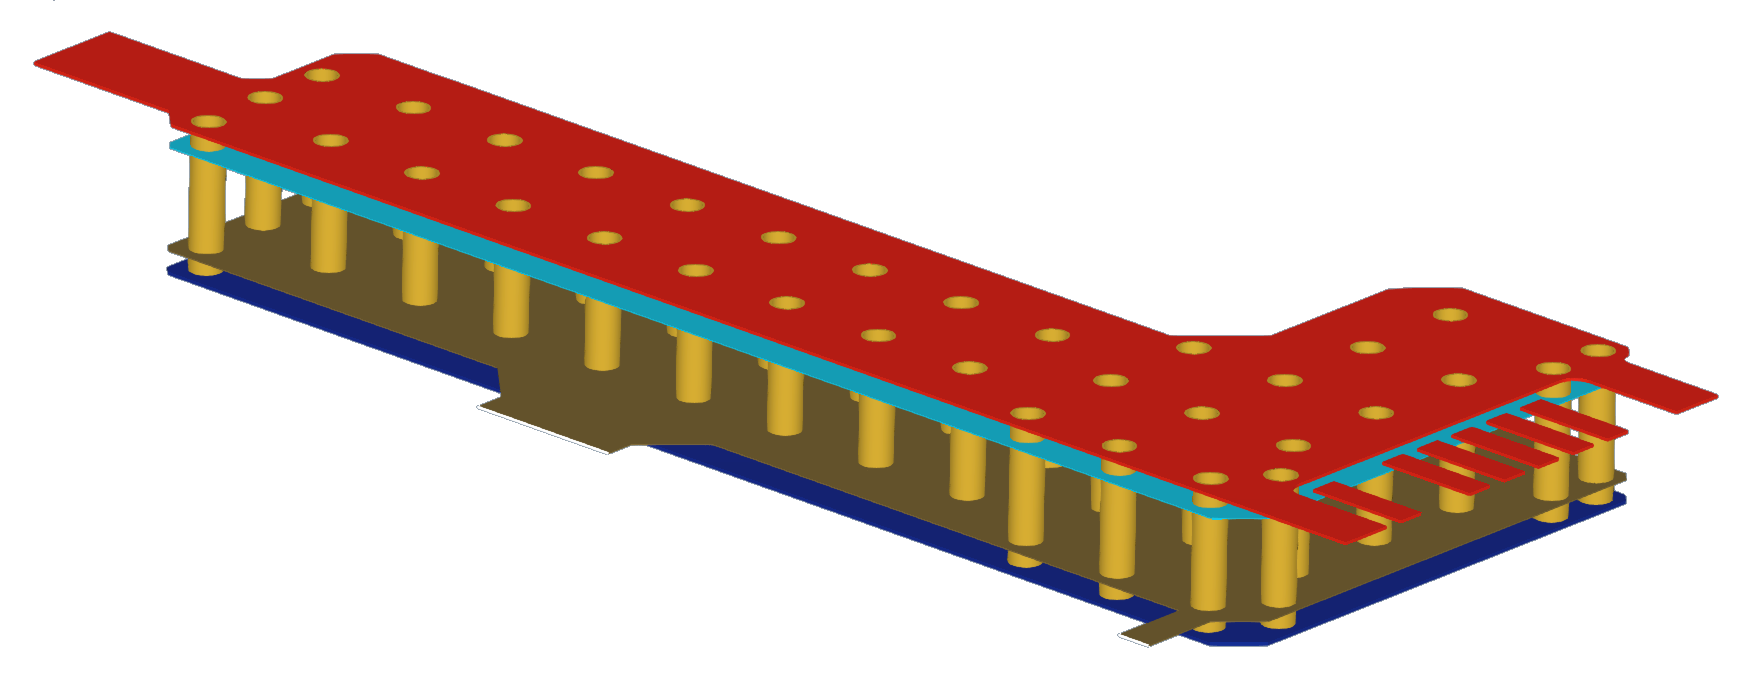
\includegraphics[width=0.9\textwidth]{figures/2_HW_figures/main_bus_section.png}
            \caption{Copper polygon pours and via stitching used for the high-current VBUS.}
            \label{fig:main_bus_layout}
        \end{figure}


        
    \subsubsection{Switching Power Supply (DC/DC)}
    The layout of the MAX77597 step-down converter focuses on minimizing Electromagnetic Interference (EMI) and parasitic ringing. The input capacitor ($C_{IN}$) and output capacitor ($C_{OUT}$) are placed as physically close to the IC pins as possible. This tight placement minimizes the area of the high $di/dt$ switching loops. The inductor is positioned immediately adjacent to the switching node (LX) pin to keep the noisy copper area small, reducing capacitive coupling to nearby analog traces. 

    Furthermore, the layout strictly implements the grounding isolation strategy established during the schematic design phase (see Section~\ref{sec:schematic_max77597}). Because the high-current switching action induces significant voltage transients on the power return path, the Analog Ground (AGND) and Power Ground (PGND) are physically separated on the top layer. The exposed thermal pad (EP) and the returns for the high-current components ($C_{IN}$ and $C_{OUT}$) are tied directly to the main GND plane. Conversely, the sensitive internal \SI{5}{\volt} BIAS regulator capacitor is referenced exclusively to the quiet AGND pin using an isolated trace. To prevent ground loops while establishing a common system reference, these two distinct ground domains are tied together at a single point, forming a star-ground topology. The star point is located directly at the negative thermal pad of the IC, as recommended in the device datasheet~\cite{max77597_datasheet} and illustrated in Figure~\ref{fig:dcdc_layout}. This approach minimizes ground-loop currents, reduces coupling between noisy and sensitive return paths, and ensures a controlled reference potential for the entire system.

    \begin{figure}[H]
    \centering
        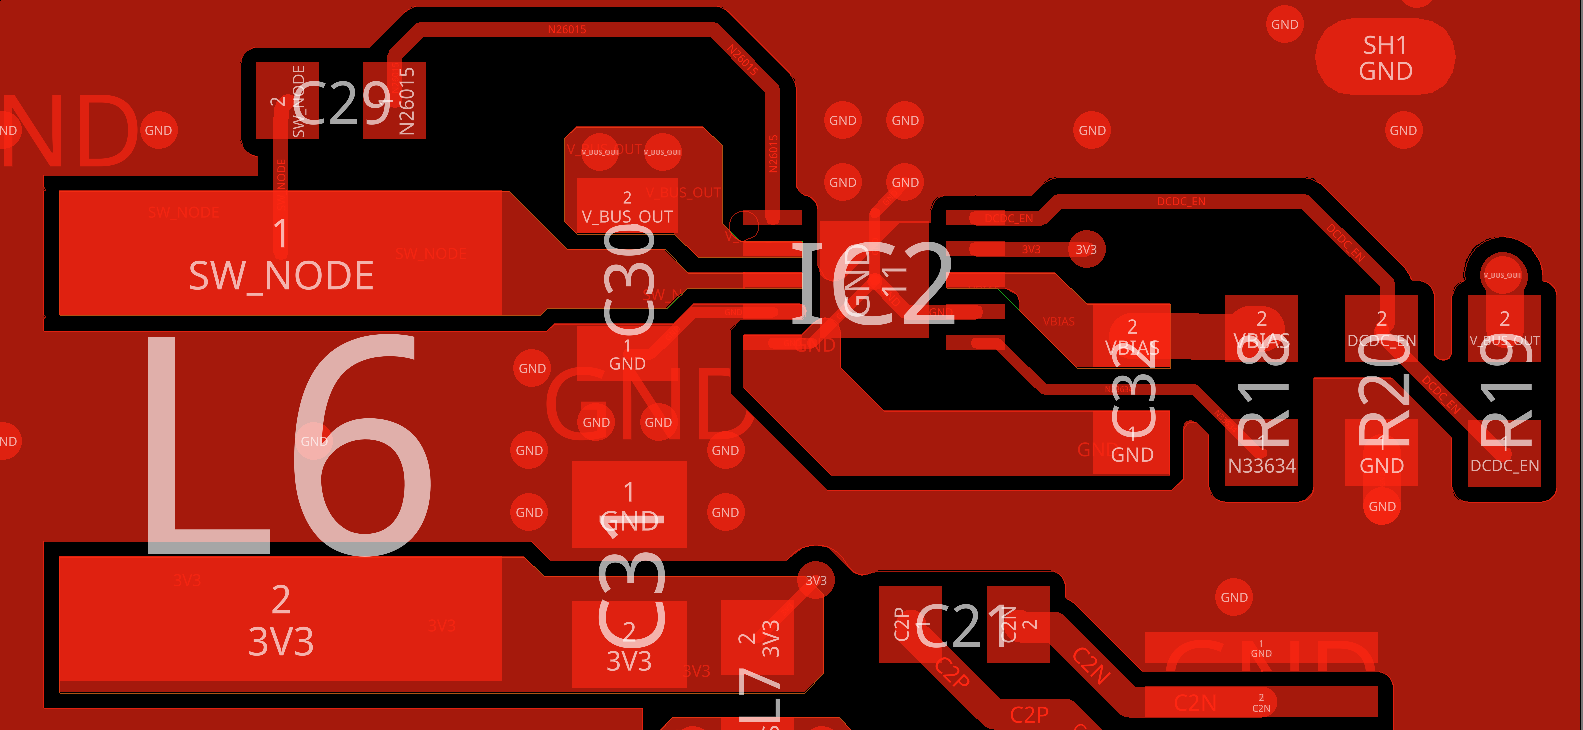
\includegraphics[width=0.9\textwidth]{figures/2_HW_figures/dcdc_layout.png}
        \caption{PCB layout of the MAX77597 step-down converter.}
        \label{fig:dcdc_layout}
    \end{figure}


    \subsubsection{RF Matching Network and Antenna}
    As established in the component placement strategy section \ref{component_placement_strategy}, the IFA antenna and its matching network are strategically positioned at the edge of the PCB to maximize their physical separation from the high-frequency switching noise generated by the DC/DC converter. This placement also creates a dedicated area free from sensitive circuitry, reducing the risk of RF noise coupling.

    The \SI{2.4}{\giga\hertz} Bluetooth transmission requires meticulous impedance control to ensure maximum power transfer and minimal signal reflection. The trace connecting the MCU RF pins to the PCB antenna is routed as a controlled \SI{50}{\ohm} impedance line using a Coplanar Waveguide with Ground (CPWG) structure. To isolate this sensitive transmission line from internal board noise and prevent electromagnetic leakage, a layout technique known as "via fencing" was applied. As shown in Figure~\ref{fig:rf_layout}, the top-layer ground pours flanking the RF trace are heavily populated with a continuous row of vias connecting directly to the solid internal L2 ground plane. This creates a protective electromagnetic boundary, functioning similarly to a coaxial cable embedded within the PCB.

    Additionally, the passive components comprising the impedance matching network are placed in a tightly packed geometry directly between the MCU and the antenna feed point. This minimizes any uncalculated parasitic inductance or capacitance that could detune the network. Finally, to allow the antenna to radiate efficiently into free space, "keep-out" zones were created. The PCB area directly beneath and immediately surrounding the antenna is entirely devoid of copper on all layers (Top, In1, In2, and Bottom) to prevent signal absorption and impedance mismatch. For the same reason, the components placed in close proximity to the antenna section ($S2$ and $J4$) are intended exclusively for testing and debugging purposes. These components are included to facilitate testing and validation during the development phase. In the final product, they will not be populated, thereby increasing the clearance area around the antenna and further reducing undesired degradation of the transmitted signal.

    \begin{figure}[htbp]
        \centering
        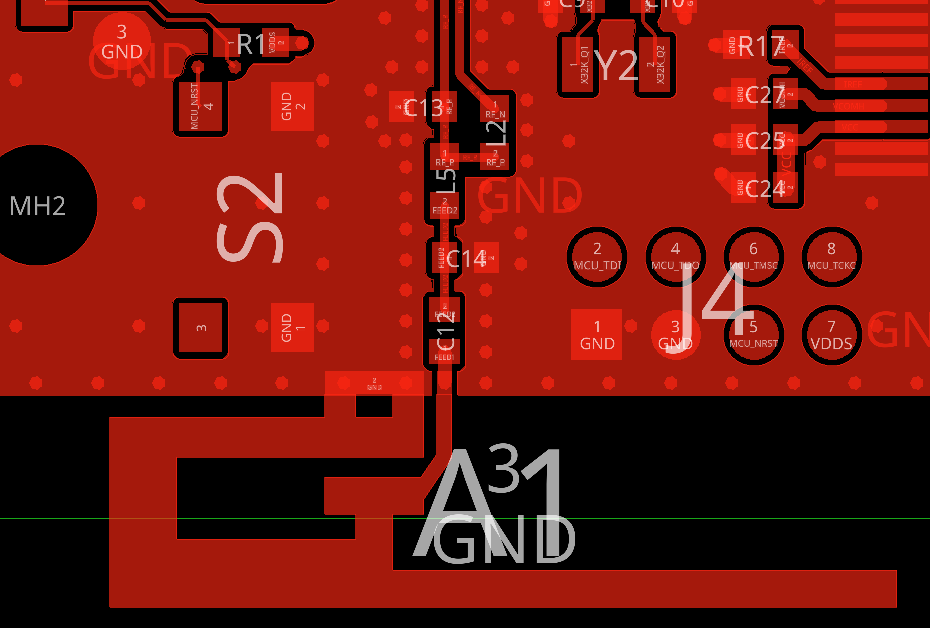
\includegraphics[width=0.9\textwidth]{figures/2_HW_figures/rf_layout.png}
        \caption{PCB layout of the RF subsystem, illustrating the tightly grouped matching network, the via fencing and the copper keep-out zone surrounding the antenna.}
        \label{fig:rf_layout}
    \end{figure}


    \subsubsection{Precision Analog Measurement}
    Accurate power measurement relies heavily on the layout of the PAC1951 and its associated \SI{10}{\milli\ohm} shunt resistor. To ensure that current measurement noise is minimized, the sense traces connecting the shunt resistor to the PAC1951 inputs are routed using the Kelvin connection terminals, available on the $R10$ package. These traces are tapped directly from the inner edges of the resistor pads to bypass the voltage drop introduced by high-current solder joints. Furthermore, the sense lines are routed as a tightly coupled differential pair and the PAC1951 input differential filter is placed with a symmetrical layout to minimize any mismatch between the two sensing paths.

    Figure~\ref{fig:kelvin_connection} illustrates the implemented Kelvin sensing layout used in the design.

    \begin{figure}[H]
        \centering
        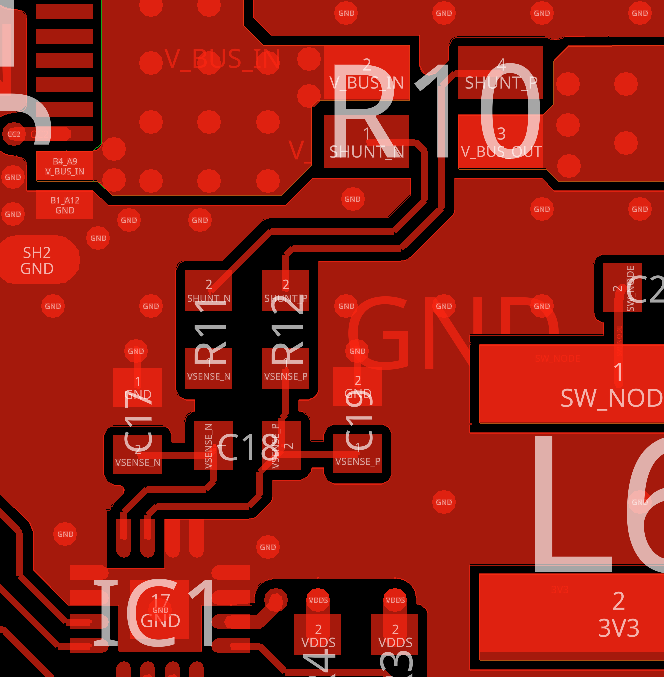
\includegraphics[width=0.65\textwidth]{figures/2_HW_figures/kelvin_connection.png}
        \caption{Kelvin connection layout of the $R10$ shunt resistor and PAC1951 sensing inputs.}
        \label{fig:kelvin_connection}
    \end{figure}


\subsubsection{Display Placement}

The physical placement and routing of the display required careful mechanical consideration to maximize usable board space while maintaining an ergonomic user interface. Rather than placing the bulky display on the already densely populated top layer, the flexible connector was strategically mounted on the right side of the board, in order for the display to be bent towards the back side of the pcb, where no SMD components are mounted, as shown in Figure~\ref{fig:display_placement}. To avoid increasing the overall PCB length and to eliminate the need for rerouting to accommodate additional clearance, the display module is placed in close proximity to the TH JTAG programming connector. This arrangement does not create any functional issues because, during the development and testing phase, the display is intentionally left non folded in its final position, allowing simultaneous access to the programming connector and full visibility of the display. In the final product, the JTAG connector is not populated leaving sufficient space for the display to be permanently attached on the back side of the board.

Mechanically, the flexible flat cable of the OLED display is routed around the edge of the PCB to connect the display module mounted on the opposite side of the assembly. To protect the delicate flexible connection from excessive bending stress and potential damage, a rounded-edge cutout is incorporated into the PCB directly beneath the cable path, allowing the cable to remain within the overall PCB outline.

\begin{figure}[H]
    \centering
    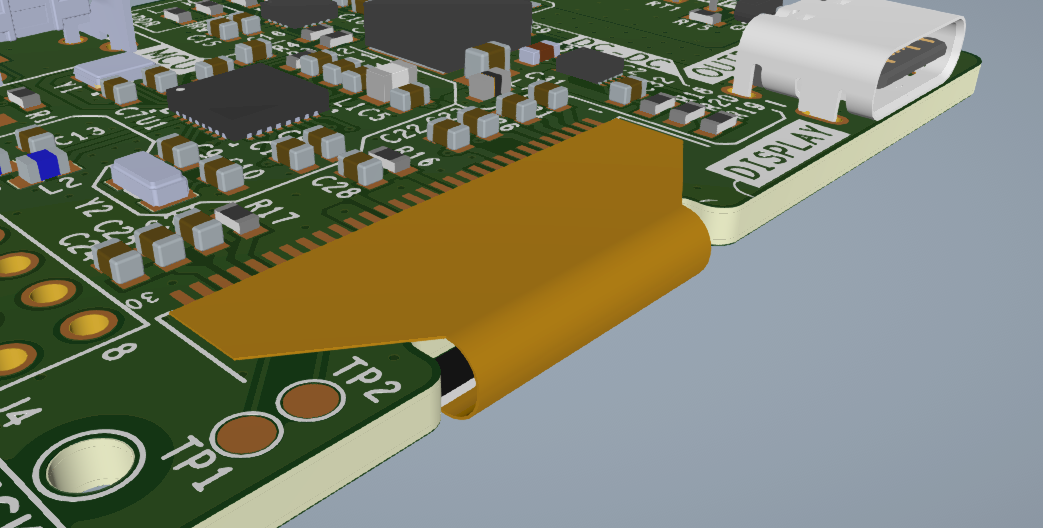
\includegraphics[width=0.8\textwidth]{figures/2_HW_figures/3d_display_top.png}
    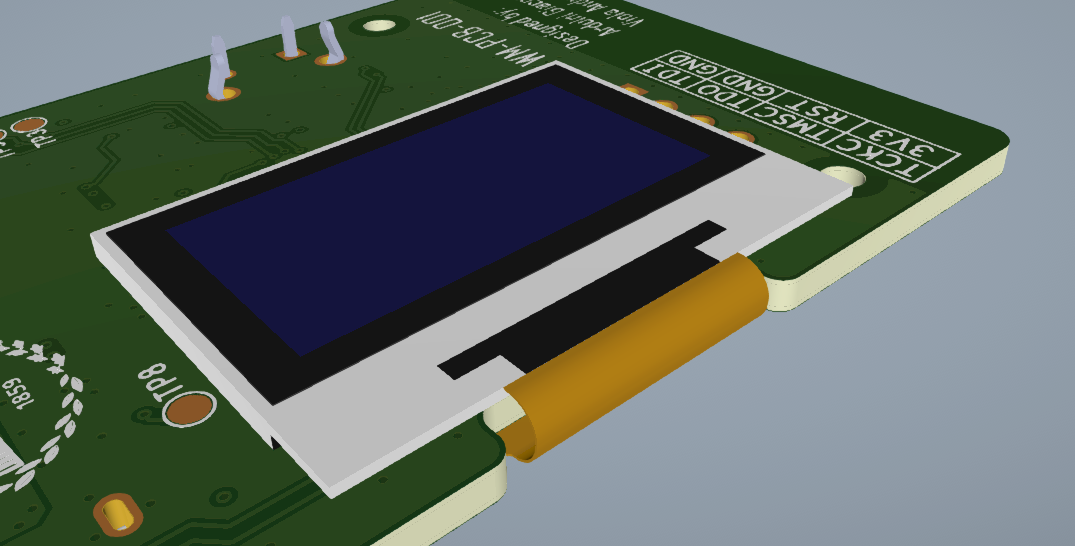
\includegraphics[width=0.8\textwidth]{figures/2_HW_figures/3d_display_bottom.png}
    \caption{Display connector placement and routing strategy showing the display folding towards the back side of the PCB.}
    \label{fig:display_placement}
\end{figure}


\subsubsection{Grounding Strategy}

Via usage in the PCB layout follows a hierarchical strategy, starting from local component-level optimization and extending to global plane interconnection across the 4-layer stack-up introduced in Section~\ref{stackup}.

At the local level, vias are placed in close proximity to high-speed and sensitive components (see Figure~\ref{fig:local_via_decoupling}). This includes ground vias adjacent to IC power pins, decoupling capacitors, and mixed-signal devices. The primary objective of this placement is to minimize current loop areas, reduce parasitic inductance, and improve high-frequency decoupling effectiveness.

In addition to local grounding, a broader via stitching strategy is applied across the entire PCB (see Figure~\ref{fig:via_stitching_detail}). This technique interconnects the copper planes defined in the 4-layer stack-up, ensuring a continuous low-impedance path between ground and power domains. From a thermal perspective, via arrays provide vertical heat conduction paths that improve heat spreading across the PCB thickness, reducing localized hot spots in high-current regions such as VBUS and GND distribution networks. From an electrical perspective, via stitching reduces ground impedance and minimizes inductive discontinuities between layers. This is particularly important for high-frequency switching currents and RF-sensitive sections, where uncontrolled return paths can lead to electromagnetic interference and degraded performance.

\begin{figure}[H]
    \centering
    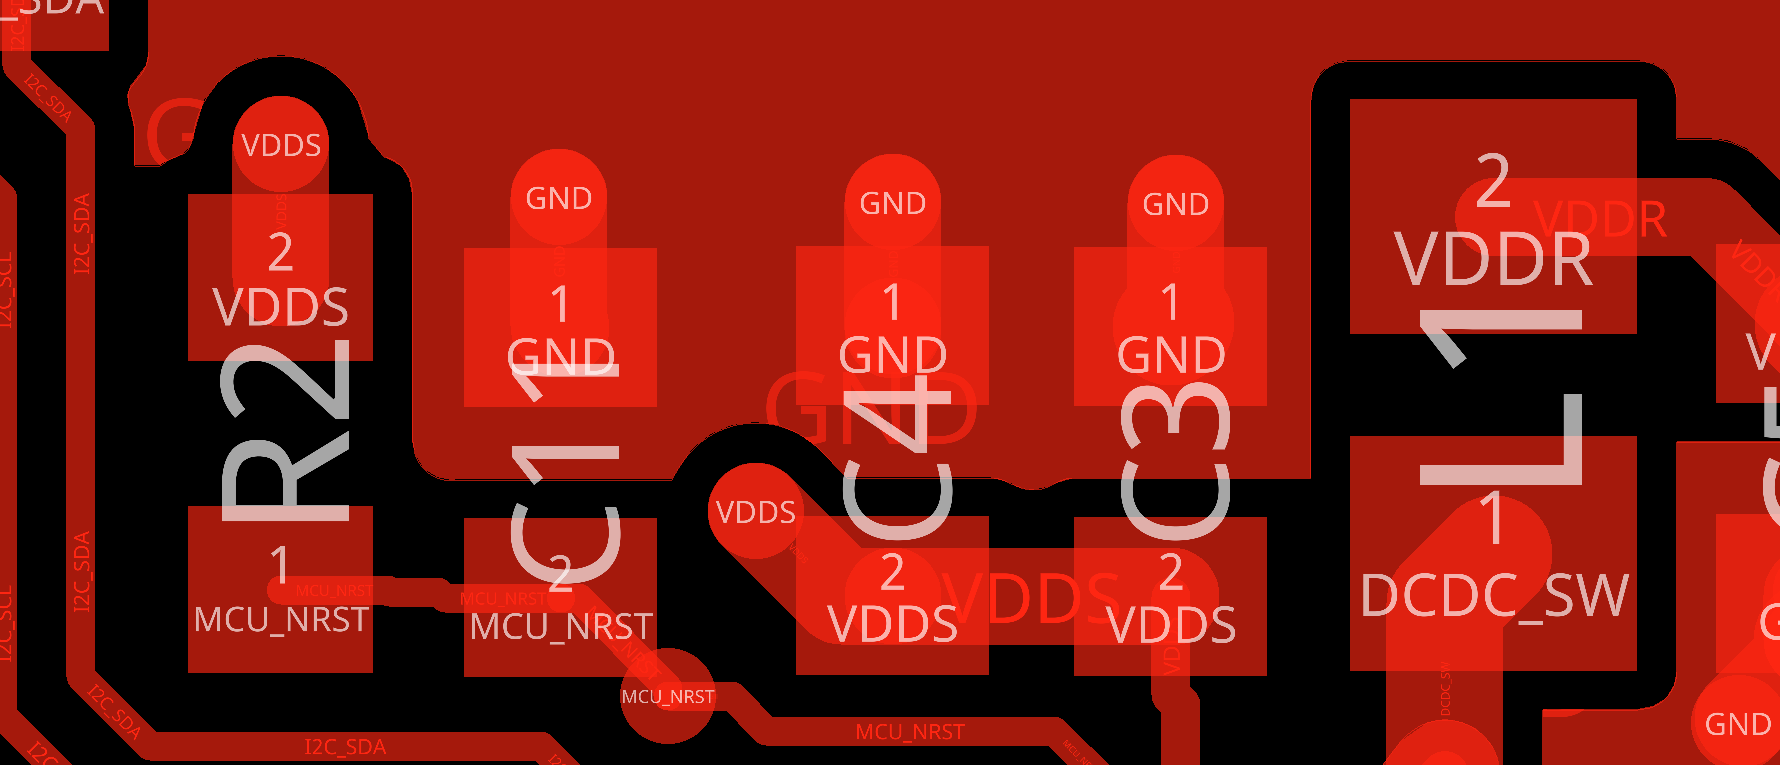
\includegraphics[width=0.75\textwidth]{figures/2_HW_figures/local_via_decoupling.png}
    \caption{Local placement of ground vias near IC power pins and decoupling capacitors to minimize loop inductance and improve high-frequency decoupling performance.}
    \label{fig:local_via_decoupling}
\end{figure}

\begin{figure}[H]
    \centering
    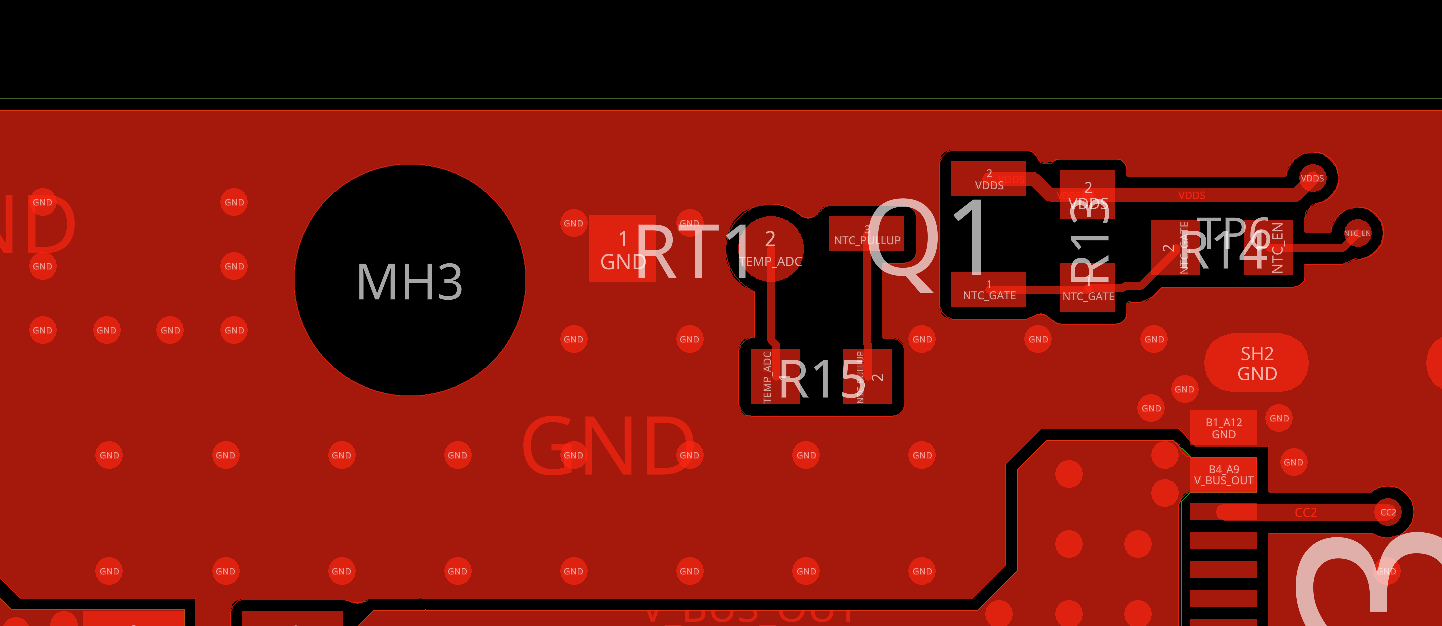
\includegraphics[width=0.85\textwidth]{figures/2_HW_figures/via_stitching_detail.png}
    \caption{Detail of the global via stitching strategy used to interconnect ground planes across the 4-layer stack-up.}
    \label{fig:via_stitching_detail}
\end{figure}






%--------------------------------------------------
% Firmware Design
\chapter{Firmware Design}
This chapter describes the firmware design principles adopted for WattMate. The implementation was mainly driven by the following objectives:

\begin{itemize}
	\item \textbf{Energy efficiency.}
	Since WattMate is intended to operate as a battery-powered embedded device, the firmware avoids unnecessary activity whenever the current system state does not require it.
	
	\item \textbf{Reliable measurement acquisition.}
	Electrical and temperature measurements are sampled at the required rate, processed consistently, and made available to the rest of the system while avoiding unnecessary latency, stale data and loss of information.
	
	\item \textbf{Responsive user interaction.}
	The local display reflects the current device state, while user inputs and BLE interactions are handled with sufficiently low latency to provide predictable behavior during normal operation.
\end{itemize}


\section{Architecture Overview}

The WattMate firmware is organized into three main layers: \texttt{device drivers}, \texttt{application tasks} and \texttt{RTOS kernel}.

\texttt{Device drivers} provide the interface between the application code and the hardware resources of the system. These resources include both internal MCU peripherals and external devices, such as the SSD1306 OLED display controller and the PAC1951 voltage/current sensor. The purpose of the drivers is to expose a simple and consistent API to the application layer, hiding the low-level hardware operations required to configure and access each peripheral.

The \texttt{application code} implements the main functionalities of WattMate by using the APIs exposed by the drivers. It is divided into multiple threads, referred to in this report as \texttt{tasks}, each responsible for a specific part of the system. Tasks communicate with each other through application events, delivered using the RTOS mechanisms of \textit{Mailboxes}. This approach avoids direct blocking calls between modules of the application code and keeps each task responsible for its own internal state. It also improves modularity, since each subsystem can be developed and maintained with limited dependencies on the others.

The task-based structure allows the RTOS to schedule the different firmware activities according to their priority and timing requirements. This is especially important for time-sensitive operations, such as BLE communication and periodic sensor acquisition. Each task is designed to avoid busy-waiting: when no operation has to be performed, the task sleeps until specific wake-up conditions instead of executing polling loops. This allows the RTOS to schedule the system efficiently and enables the power management policy to enter low-power modes whenever possible.

\begin{table}[H]
	\centering
	\caption{Overview of the main firmware levels.}
	\label{tab:firmware_levels}
	\begin{tabular}{lll}
		\toprule
		\textbf{Level} & \textbf{Role} & \textbf{Examples} \\
		\midrule
		Drivers & Hardware abstraction & PAC1951 driver, SSD1306 driver, ... \\
		App. Tasks & System functionality & Acquisition, Display, BLE, Flash, ... \\
		RTOS & Scheduling and Synchronization & Mailboxes, Sleep management, ... \\
		\bottomrule
	\end{tabular}
\end{table}

\paragraph{Original and external firmware components}
The \texttt{RTOS kernel} and the low-level MCU peripheral drivers are provided by Texas Instruments and were not modified. They were only respectively configured through the \texttt{.cfg} configuration file and the board support file (\texttt{startup/board.h}). The original code developed for this project mainly consists of the application tasks, the BLE data handling logic, the Flash storage logic, and the PAC1951 driver, for which no open-source C driver was found. The SSD1306 display driver was adapted from existing open-source C implementations and extended with project-specific APIs.

For this reason, the following sections focus mainly on the original firmware components developed for WattMate. External or vendor-provided code is discussed only when its behavior is relevant to explain a specific design choice.

\section{Application Tasks}

The application-level tasks used to implement the WattMate firmware are located mainly in 
\texttt{WattMate\_BLE/Startup/Tasks} and \texttt{WattMate\_BLE/Application}. 
They are listed below:

\begin{itemize}
	\item \textbf{App:}
	This is the main application task. It maintains and updates the global state of the device by processing events received from the other tasks and coordinating the behavior of the different subsystems according to runtime policies. In general, the App task does not handle low-level hardware details directly; instead, it sends high-level requests to the other tasks, which are responsible for executing them in the appropriate timing and hardware context.
	
	\item \textbf{Display:}
	This task handles the OLED Display user interface. It receives commands from the App task, which controls the general display state. The Display task stores the layout of each visible page, manages screen updates, animations and standby timing, and exclusively owns the SSD1306 driver handling.
	
	\item \textbf{Flash Storage:}
	This task manages persistent firmware-produced data stored in the internal Flash memory. It exposes APIs to store and retrieve the data records, while hiding the details of Flash page organization, record placement, writing, validation, and erase handling from the rest of the application.
	
	\item \textbf{Input:}
	This task manages inputs that are handled by internal MCU peripherals. It handles the user button, including debounce and long-press detection, and controls the ADC sampling and NTC Enable output GPIO used to read the NTC temperature sensor. The App task is notified only when a relevant input event or a new temperature sample is available, avoiding continuous polling.
	
	\item \textbf{PAC:}
	This task manages the acquisition flow of the PAC1951 sensor. It receives high-level requests from the App task and configures the timing and sensor settings according to predefined sampling profiles. When a new electrical measurement is obtained from the PAC1951 driver, the App task is notified through an event, avoiding continuous polling.
	
	\item \textbf{WattMate BLE:}
	This task manages the BLE interface of WattMate. It handles advertising, connection state changes, the custom GATT service, telemetry notifications, and control/configuration commands received from the mobile application. BLE events that affect the device behavior are translated into application events and forwarded to the App task.
	
	
\end{itemize}

\subsection{Task Communication Model}

Communication between firmware tasks is mainly based on event messages. When a task, a timer callback, or an interrupt callback needs to notify another part of the system, it posts an event message into the mailbox of the destination task. The receiving task sleeps while no message is pending on its mailbox, so no busy-waiting loop is required. Once a pending message arrives in the mailbox of a task, the task is woken up according to its priority assigned in the RTOS scheduler, and the required operations can be performed.

\begin{figure}[H]
	\centering
	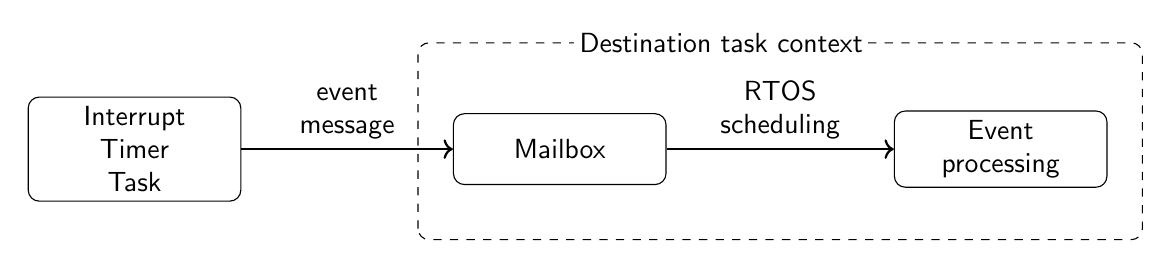
\begin{tikzpicture}[
		block/.style={
			draw,
			rounded corners,
			align=center,
			minimum height=0.9cm,
			minimum width=2.7cm
		},
		context/.style={
			draw,
			rounded corners,
			dashed
		},
		arrow/.style={->, thick}
		]
		
		```
		% Blocks
		\node[block] at (0,0) (source) {Interrupt\\Timer\\Task};
		\node[block] at (5.4,0) (mailbox) {Mailbox};
		\node[block] at (11,0) (processing) {Event\\processing};
		
		% Destination task context
		\draw[context] (3.6,-1.15) rectangle (12.8,1.35);
		\node[fill=white, inner sep=2pt] at (7.45,1.35) {Destination task context};
		
		% Arrows
		\draw[arrow] (source.east) -- node[above, align=center] {event\\message} (mailbox.west);
		\draw[arrow] (mailbox.east) -- node[above, align=center] {RTOS\\scheduling} (processing.west);
		
	\end{tikzpicture}
	\caption{Event-based communication model between firmware tasks.}
	\label{fig:task_communication_model}
	
\end{figure}

This model avoids busy-waiting loops and reduces direct dependencies between modules. Interrupt and timer callbacks are kept short, since they only post the corresponding event message, while the actual processing is deferred to the destination task context.

\subsection{Task Scheduling and Priorities}

The event-based communication model only defines how tasks are notified. The actual execution order of tasks that simultaneously require CPU time is still controlled by the TI-RTOS scheduler. In practice, when a message is posted to the mailbox of a blocked task, that task becomes ready to execute, but this does not necessarily mean that it immediately receives CPU time. The scheduler selects which ready task is executed according to the configured scheduling policy~\cite{ti_sysbios_user_guide}, based on task priorities.


This behavior is exploited in the firmware design to separate tasks with different characteristics, with the final goal of guaranteeing the correct behavior of the whole system, from the time-sensitive functionalities to the ones that can handle a longer latency. The idea is that the system must remain responsive to external inputs, while the internal computations can wait for the CPU to be available before being performed.

The resulting priority assignment is summarized in Table~\ref{tab:task_priorities}. In TI-RTOS, task priorities are numeric and increase with the assigned value; therefore, a task with priority 3 has higher priority than a task with priority 2 or 1~\cite{ti_sysbios_task}.

\begin{table}[H]
	\centering
	\small
	\setlength{\tabcolsep}{4pt}
	\renewcommand{\arraystretch}{1.25}
	\caption{Firmware task priority assignment.}
	\label{tab:task_priorities}
	\begin{tabularx}{\textwidth}{
			@{}
			>{\raggedright\arraybackslash}p{2.3cm}
			>{\centering\arraybackslash}p{1.5cm}
			>{\raggedright\arraybackslash}X
			@{}
		}
		\toprule
		\textbf{Task} &
		\textbf{Priority} &
		\textbf{Design rationale}
		\tabularnewline
		\midrule
		
		BLE & 3 &
		Must remain as responsive as possible in order to satisfy the strict time constraints of the BLE protocol, maintain the connection, and exchange data with the mobile application.
		\tabularnewline
		
		PAC & 2 &
		Electrical measurements are part of the core monitoring function and should be handled with limited latency.
		\tabularnewline
		
		Input &	2 &
		User input should be processed quickly enough to make the device feel responsive. In addition, the ALERT input from the PAC1951 should be handled as quickly as possible, in order to respond quickly to dangerous situations.
		\tabularnewline
		
		App & 1 &
		Coordinates the main application logic, but it does not contain time-sensitive handling.
		\tabularnewline
		
		Flash Storage & 1 &
		Flash operations are marginal from the point of view of pure functionality, and can therefore tolerate latency if necessary.
		\tabularnewline
		
		Display & 1 &
		Display updates are human-facing operations and can tolerate small delays without being noticed by the user.
		\tabularnewline
		\bottomrule
	\end{tabularx}
	
\end{table}

The priority assignment therefore defines the practical behavior of the event-driven architecture. A low-priority task can be woken up by a message and still wait before running if higher-priority tasks are ready at the same time. As a result, heavier computations, such as SoC and SoH estimation, can coexist with time-sensitive activities, such as BLE handling, without introducing direct blocking effects or noticeable misbehaviors.

It is important to note that the scheduler is not modified by the project, and the stock TI-RTOS one is used; only the task priorities and the event-based execution structure are configured to match the firmware requirements.


\subsection{Main Application Task}
\label{Main_Application_Task}

The App task is the central coordination point of the WattMate firmware. Its main role is to maintain the global application state and to decide how the other subsystems should behave according to the current operating condition. For this reason, it receives events from the PAC, Input, Display, Flash Storage and BLE tasks, updates its internal state, and sends high-level requests back to the appropriate subsystem when an action is required.

\paragraph{Runtime resource policy.}
One of the main responsibilities of the App task is handle all the resources avaiable, in order to reduce as much as possible the power consumption. The firmware does not keep all measurements and data streams permanently active. In particular the following policies are applied:
\begin{itemize}
	\item \textbf{PAC1951 sampling profile.}
	The PAC1951 sampling profile controls the internal behavior of the sensor itself, independently from whether the MCU is currently reading data from it through I2C. The App task requests the PAC1951 \texttt{normal profile} only when electrical activity is present on the power bus; otherwise, it requests the \texttt{idle profile}.
	
	It is important to note that the \texttt{idle profile} is not simply a deep-sleep mode for the PAC1951. Even in this state, the sensor remains configured to monitor the battery line and to generate an alert when relevant electrical activity is detected again. This alert mechanism is necessary because the MCU does not always read the PAC1951 continuously through I2C; therefore, when I2C communication is suspended, the MCU has no direct information about the current state of the power bus. The PAC1951 alert pin provides a notification that the bus has become active again, allowing the firmware to wake up the corresponding logic, re-evaluate the system state, and request the PAC1951 \texttt{normal profile} if when needed. More details about the two PAC profiles are provided in Section~\ref{PAC_Application_Task}.
	
	
	\item \textbf{PAC1951 measurement stream.}
	The measurement stream controls the I2C communication between the MCU and the PAC1951. When the stream is enabled, the PAC task periodically reads the latest electrical measurements from the sensor through the I2C bus and forwards updated snapshots to the App task. When the stream is disabled, the PAC1951 can still keep its configured sampling profile, but the MCU avoids periodic I2C transactions.
	
	The stream is enabled only when live electrical measuremet data are needed by the rest of the system, such as when the display is on, or when the BLE application is requesting telemetry. If none of these conditions is true, the stream is released, allowing the MCU to remain in sleep mode for longer periods and helping the RTOS power policy enter deep low-power states.
	
	\item \textbf{Temperature ADC sampling.}
	Similarly to the Electrical PAC1951 measures, the NTC temperature measurement is also managed as an on-demand resource. The ADC sampling is enabled in the Input Task only when temperature information is needed, for example when the display is currently showing a page that requires temperature data, or when the BLE application is requesting live telemetry. This allows the MCU to remain in sleep mode for longer periods and helps the RTOS power policy enter deep low-power states.
	
	\item \textbf{Energy accumulation.}
	PAC1951 energy accumulation I2C reading, performed by the PAC Task, is enabled only when the accumulated energy is useful for the current firmware state, for example when the display or BLE interface requires energy-related information. Separating live electrical measurements from energy accumulation allows the firmware to avoid unnecessary I2C communications.
	
	\item \textbf{Display dimming and standby.}
	The OLED display is not kept fully active permanently. After a period without user interaction (\SI{20}{s}), the App task requests a low-luminosity state for the display. If the inactivity continues for an additional \SI{10}{s}, the display is turned off. A user button press wakes up the display again.
	
	This policy reduces the system power consumption in both a direct and an indirect way. Directly, dimming or turning off the display lowers the energy required by the OLED itself. Indirectly, the display state also influences the rest of the runtime policy: when the display is completely off, live measurement streams are kept active only if they are still required by another subsystem, such as the BLE application. In this way, the firmware avoids keeping acquisition and update activity enabled only for a user interface that is not currently visible.
	
	
	
	\item \textbf{BLE advertising.}
	BLE advertising is enabled only when the device must be discoverable, therefore when no active BLE connection is open. The advertising frequency is also dynamically changed by the firmware: fast advertising (\SI{100}{ms} period) is used for a limited time (\SI{20}{s} period) at startup and after a user button press, while slow advertising (\SI{1}{s} period) is used in the remaining conditions. This keeps the device available for connection, although with longer discovery times, while reducing the power consumption associated with BLE when the user is not actively interacting with WattMate.
	
	\item \textbf{BLE data stream.}
	BLE telemetry streaming is enabled only when requested by the mobile application. This prevents the firmware from continuously preparing and sending BLE notifications when no client is actively using live data.
	
	\item \textbf{BLE connection supervision.}
	The BLE connection is kept active as long as the central device remains reachable. The firmware does not require a continuous application-level data exchange to maintain the connection; this is handled by the BLE link layer. However, if the phone becomes unreachable, for example because it is turned off or moved out of range, the connection eventually expires through the BLE supervision timeout (\SI{2}{s}). In that case, the firmware processes the disconnection event and returns WattMate to the advertising state, instead of remaining associated with a non-responsive device.
	
\end{itemize}

\paragraph{Measurement freshness.}
Considering the Resource Policies, it is clear that the App task has no guarantee to receive a constant stream measured data at all times. Because of this, App task keeps track of the validity of the latest measurements. Electrical, energy, and temperature data are marked as fresh only for a limited time after a new sample is received. If no updated sample arrives before the corresponding timeout expires, the data are marked as not fresh, preventing the display, BLE telemetry, and battery estimation logic from using outdated values as if they were current measurements.

\begin{table}[H]
	\centering
	\small
	\caption{Measurement data freshness timeouts}
	\label{tab:data_freshness}
	\begin{tabular}{ll}
		\toprule
		\textbf{Measurement Type} & \textbf{Timeout} \\
		\midrule
		PAC Live Data  & 500 ms  \\
		PAC Energy     & 500 ms  \\
		Temperature    & 2000 ms \\
		\bottomrule
	\end{tabular}
\end{table}

\paragraph{Battery operating conditons.}
The App task is responsible for estimating the battery-related statistics used by WattMate. The firmware first reconstructs the operating condition of the battery by detecting charge and discharge sessions from the PAC1951 measurements. The same data are then processed to update energy, State of Charge, State of Health, and cycle-related information.

A session is detected from the instantaneous power measured on the power bus. The firmware compares the measured power with predefined start and stop thresholds to determine whether the battery is being charged (state \texttt{CHARGE}), discharged (state \texttt{DISCHARGE}), or if no active session is present (state \texttt{IDLE}). The use of separate start and stop thresholds introduces hysteresis, preventing unstable transitions caused by small power fluctuations around zero.

When the measured power falls below the corresponding stop threshold, the session is moved to \texttt{PAUSED} instead of being immediately closed. The session is terminated only if the inactive condition persists until the timeout expires, allowing short interruptions to be tolerated without splitting a single physical charge or discharge process into multiple independent sessions.

This behavior is summarized by the finite-state machine shown in Figure~\ref{fig:session_fsm}.

\begin{figure}[H]
	\centering
	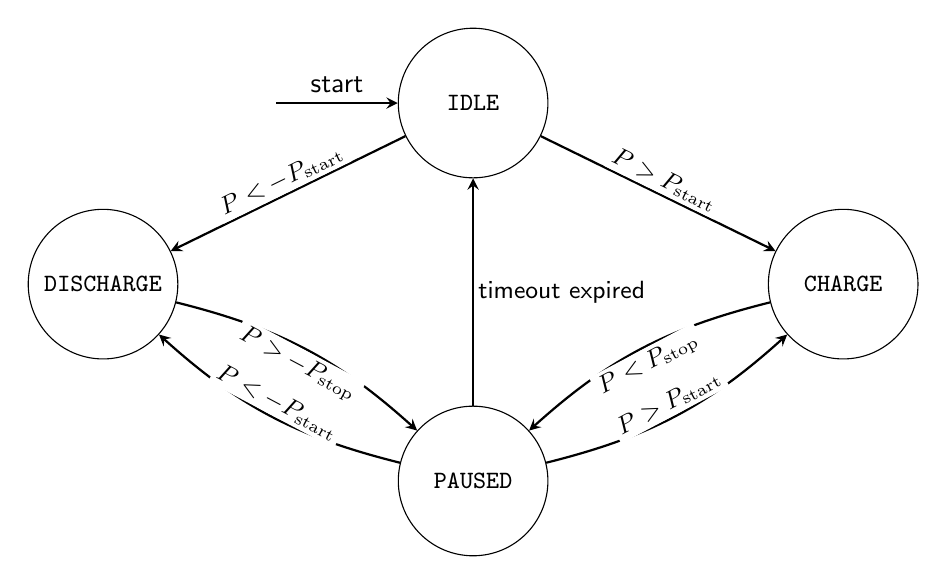
\begin{tikzpicture}[
		>=stealth,
		state/.style={
			draw,
			circle,
			minimum size=1.9cm,
			inner sep=1pt,
			align=center,
			font=\small\ttfamily
		},
		trans/.style={->, thick},
		lab/.style={
			font=\small,
			fill=white,
			inner sep=1.5pt
		}
		]
		
		% States
		\node[state] (idle) at (0,3.0) {IDLE};
		\node[state] (charge) at (4.7,0.7) {CHARGE};
		\node[state] (discharge) at (-4.7,0.7) {DISCHARGE};
		\node[state] (paused) at (0,-1.8) {PAUSED};
		
		% Initial arrow
		\draw[trans] (-2.5,3.0) -- node[above] {start} (idle.west);
		
		% Session start
		\draw[trans] (idle) -- node[lab, above, sloped] {$P > P_{\mathrm{start}}$} (charge);
		\draw[trans] (idle) -- node[lab, above, sloped] {$P < -P_{\mathrm{start}}$} (discharge);
		
		% Charge pause / resume
		\draw[trans] (charge) to[bend right=14]
		node[lab, below, sloped] {$P < P_{\mathrm{stop}}$}
		(paused);
		
		\draw[trans] (paused) to[bend right=14]
		node[lab, above, sloped] {$P > P_{\mathrm{start}}$}
		(charge);
		
		% Discharge pause / resume
		\draw[trans] (discharge) to[bend left=14]
		node[lab, below, sloped] {$P > -P_{\mathrm{stop}}$}
		(paused);
		
		\draw[trans] (paused) to[bend left=14]
		node[lab, above, sloped] {$P < -P_{\mathrm{start}}$}
		(discharge);
		
		% Session termination
		\draw[trans] (paused) -- node[lab, right] {timeout expired} (idle);
		
	\end{tikzpicture}
	\caption{Finite-state machine used for session detection from the measured power.}
	\label{fig:session_fsm}
\end{figure}

\paragraph{Battery statistics estimation.}
Once a charge or discharge session has been identified, the App task uses the
session information to compute higher-level battery statistics. These quantities
are derived from the energy exchanged during detected sessions, rather than from
instantaneous voltage or current values alone.

The estimation method is based on energy integration at the USB bus. This gives
a reliable measurement of the energy that entered or left the system during a
session, but it does not directly reveal the absolute battery State of Charge.
WattMate is placed on the USB power path and does not directly observe the
battery cell voltage or the electrochemical end-of-charge/end-of-discharge
conditions. Therefore, SoC and SoH estimation require explicit operating
assumptions.

The firmware assumes that a completed charge or discharge session corresponds to
a known battery endpoint:
\[
\begin{cases}
	\texttt{CHARGE completed} & \Rightarrow \mathrm{SoC} = 100\% \\
	\texttt{DISCHARGE completed} & \Rightarrow \mathrm{SoC} = 0\%
\end{cases}
\]
This assumption provides the absolute reference point that energy integration
alone cannot provide. Before the first completed session, the SoC is therefore
marked as \texttt{UNKNOWN}. After the first completed session, the SoC is set to either 0\% or 100\%, depending on the direction of the session, and the eitimation of SoC can atually begin.

During an active session, the firmware computes the energy exchanged since the
session started, denoted as \(E_{\mathrm{session}}\). This value is compared with
the best available estimate of the usable battery energy:
\[
\mathrm{progress} =
\frac{E_{\mathrm{session}}}{E_{\mathrm{usable}}} \cdot 100
\]
The SoC is then obtained according to the session direction:
\[
\mathrm{SoC} =
\begin{cases}
	\mathrm{progress} & \text{during charge} \\
	100 - \mathrm{progress} & \text{during discharge}
\end{cases}
\]

Before a measured usable-energy reference is available, the firmware can only use
the nominal battery energy configured through BLE. In this case, the SoC is
reported as \texttt{ESTIMATED}. Once at least one completed sessions have been observed, the energy measured during a completed endpoint-to-endpoint session can be used as the usable-energy reference, and the SoC estimate can be promoted to \texttt{LEARNED}.

The \textit{State of Health} is computed by comparing the measured usable energy
with the nominal battery energy:
\[
\mathrm{SoH} =
\frac{E_{\mathrm{usable}}}{E_{\mathrm{nominal}}} \cdot 100
\]
This estimate is meaningful only if the completed session used as reference is
representative of a full usable-capacity interval. In other words, the operating
assumption is that completed charge and discharge sessions reach the actual
battery endpoints. If a session is interrupted before the battery reaches the
corresponding endpoint, the measured energy no longer represents the full usable
capacity and the SoH estimate may be biased.

The maturity of the estimates is summarized in
Table~\ref{tab:battery_estimation_maturity}.



\begin{table}[H]
	\centering
	\small
	\setlength{\tabcolsep}{4pt}
	\renewcommand{\arraystretch}{1.5}
	\caption{Battery estimation maturity during firmware operation.}
	\label{tab:battery_estimation_maturity}
	\begin{tabularx}{\textwidth}{
			@{}
			>{\raggedright\arraybackslash}p{3.0cm}
			>{\raggedright\arraybackslash}X
			>{\raggedright\arraybackslash}p{3.5cm}
			>{\raggedright\arraybackslash}p{3.5cm}
			@{}
		}
		\toprule
		\textbf{Stage} &
		\textbf{Available information} &
		\textbf{SoC status} &
		\textbf{SoH status} \\
		\midrule
		
		Startup / reset &
		Nominal battery energy (if configured from BLE); &
		\texttt{UNKNOWN}. Total energy yconsumed during first cycle is unknown. &
		\texttt{UNKNOWN}. No measured battery energy available. \\
		
		After first completed session &
		Nominal battery energy (if configured from BLE). A charge or discharge endpoint is assumed to have been reached. &
		\texttt{ESTIMATED}. SoC is computed using the nominal battery energy and Energy since the start of current session. &
		\texttt{UNKNOWN}. No measured battery energy available. \\
		
		After second completed sessions &
		Nominal battery energy (if configured from BLE), measured battery energy.  &
		\texttt{LEARNED}. SoC is computed using the last measured battery energy and current session energy  &
		\texttt{LEARNED}. SoH is computed using the last measured battery energy \\
		
		\bottomrule
	\end{tabularx}
\end{table}


\paragraph{Interaction with persistent storage.}
Persistent storage, handled by the Flash Storage Task, is used to keep the battery estimation state across resets and power cycles. Without this mechanism, WattMate would lose the learned battery history every time the device restarts, forcing the estimation process to start again from an unknown state.

The App task stores two different classes of data:

\begin{itemize}
	\item \textbf{Fast records.}
	These records are used as checkpoints for an active charge or discharge session. They store the current accumulated session energy and a small set of flags describing the state of the ongoing cycle. Fast records are written periodically, every \SI{30}{s}, instead of after every PAC1951 measurement. This limits the number of Flash write operations and reduces memory wear.
	
	If the device resets during an active session, the latest fast record can be used to restore an approximate session state. The restored energy is not considered \texttt{LEARNED}, and instead is set to \texttt{ESTIMATED}, because the checkpoint may be older than the last measurement acquired before the reset. Any energy exchanged between the last checkpoint and the reset is therefore not included in the restored value.
	
	For this reason, the firmware propagates an estimation-quality flag together with the energy values used for battery statistics. The rule is conservative: if at least one input of a calculation is \texttt{UNKNOWN}, the result is marked as \texttt{UNKNOWN}; otherwise, if at least one input is \texttt{ESTIMATED}, the result is marked as \texttt{ESTIMATED}; only values computed entirely from learned inputs are marked as \texttt{LEARNED}. The effect of this rule after a checkpoint restoration is summarized in Table~\ref{tab:checkpoint_quality_propagation}.
	
	
	\begin{table}[H]
		\centering
		\small
		\setlength{\tabcolsep}{4pt}
		\renewcommand{\arraystretch}{1.25}
		\caption{Quality propagation after checkpoint restoration.}
		\label{tab:checkpoint_quality_propagation}
		\begin{tabularx}{\textwidth}{
				@{}
				>{\raggedright\arraybackslash}p{3.cm}
				>{\raggedright\arraybackslash}X
				>{\raggedright\arraybackslash}p{3.5cm}
				>{\raggedright\arraybackslash}p{3.5cm}
				@{}
			}
			\toprule
			\textbf{Situation}					&
			\textbf{Effect on stored values}	&
			\textbf{SoC Quality} 				&
			\textbf{SoH Quality} 				\\
			\midrule
			
			Reset during an active session &
			The current-cycle energy is restored from the latest fast checkpoint and marked as \texttt{ESTIMATED}. & \texttt{ESTIMATED}, because current cycle energy is \texttt{ESTIMATED} &
			Not affected, because it uses last-session energy \\
			
			After the restored session completed &
			The completed-session energy is stored as the last completed-cycle energy, but with \texttt{ESTIMATED} quality &
			\texttt{ESTIMATED}. Starts from 0\% or 100\% with \texttt{LEARNED} current-cycle session energy, but it uses an \texttt{ESTIMATED} last-session energy &
			\texttt{ESTIMATED}. Because it uses an \texttt{ESTIMATED} last-session energy \\
			
			After the endpoint-to-endpoint session completed &
			The completed-cycle energy is measured and so it is marked as \texttt{LEARNED} &
			\texttt{LEARNED}, both current and last-session energy are \texttt{LEARNED} &
			\texttt{LEARNED}, last-session energy is \texttt{LEARNED}\\
			
			\bottomrule
		\end{tabularx}
	\end{table}
	
	
	\item \textbf{Slow records.}
	These records store the slower-changing battery estimation history. They include the nominal battery energy, the last completed cycle energy, the number of completed cycles, and the last completed session type. Slow records are updated when this higher-level state changes, mainly at the end of a session or when the battery configuration is modified via BLE.
	
	Slow records represent the learned battery history used by the firmware after a restart. They allow WattMate to preserve the estimation maturity reached during previous operation instead of returning to the initial unknown state.
\end{itemize}

The stored battery data can be cleared when the battery is replaced. This reset can be triggered either from the BLE interface or through a long press of the User Button, forcing the firmware to discard the previous battery history and rebuild the estimation state for the new battery.

\subsection{Display Application Task}

The Display Application task manages the local OLED user interface of WattMate. Its role is limited to the presentation layer: it defines the UI pages, display timing, brightness policy, screen update logic, and transitions between the different visual states. The task does not perform measurements and does not compute the values shown to the user.

The App task interacts with the Display task through high-level display commands posted to its TI-RTOS mailbox. These commands do not directly access the OLED driver or modify the rendered content; they only request UI-level actions. The detailed execution is handled internally by the Display task, which remains responsible for the UI state machine and for the SSD1306 display driver state machine. The main command categories are summarized in Table~\ref{tab:display_commands}.

\begin{table}[H]
	\centering
	\small
	\caption{Main command categories handled by the Display task.}
	\label{tab:display_commands}
	\begin{tabularx}{\textwidth}{lX}
		\toprule
		\textbf{Command category} & \textbf{Purpose} \\
		\midrule
		Initialization		& Start the display task and show the initial UI sequence. \\
		Page control		& Select the initial page or move to the next page. \\
		Brightness control	& Switch between normal and low-luminosity display modes. \\
		Power state control	& Turn the OLED display on or off. \\
		Refresh control		& Request an immediate redraw of the currently active page, over-riding the Display Task defined Refresh Rate. \\
		\bottomrule
	\end{tabularx}
\end{table}

\paragraph{Displayed data input.}
The values shown on the screen are not passed through the Display task mailbox. The mailbox is only used for high-level display commands, while the displayed data are obtained by reading a snapshot of the current application state produced by the App task.

This design reduces mailbox traffic and decouples the display refresh rate from the measurement acquisition rate. As a result, the Display task can autonomously manage UI timing, state transitions, and rendering, while always using the most recent application data available at redraw time.

\paragraph{Page organization}
The user interface is organized into a small set of pages. Similar information is
grouped together so that each page remains readable on the small OLED display:

\begin{itemize}
	\item \textbf{Live electrical measurements pages:} they show the
	live electrical measurements, namely voltage, current, power, and temperature, together with the maximum values reached during the current session.
	
	\begin{center}
		\captionsetup{type=figure,width=0.70\textwidth,font=small}
		
		\begin{minipage}{0.30\textwidth}
			\centering
			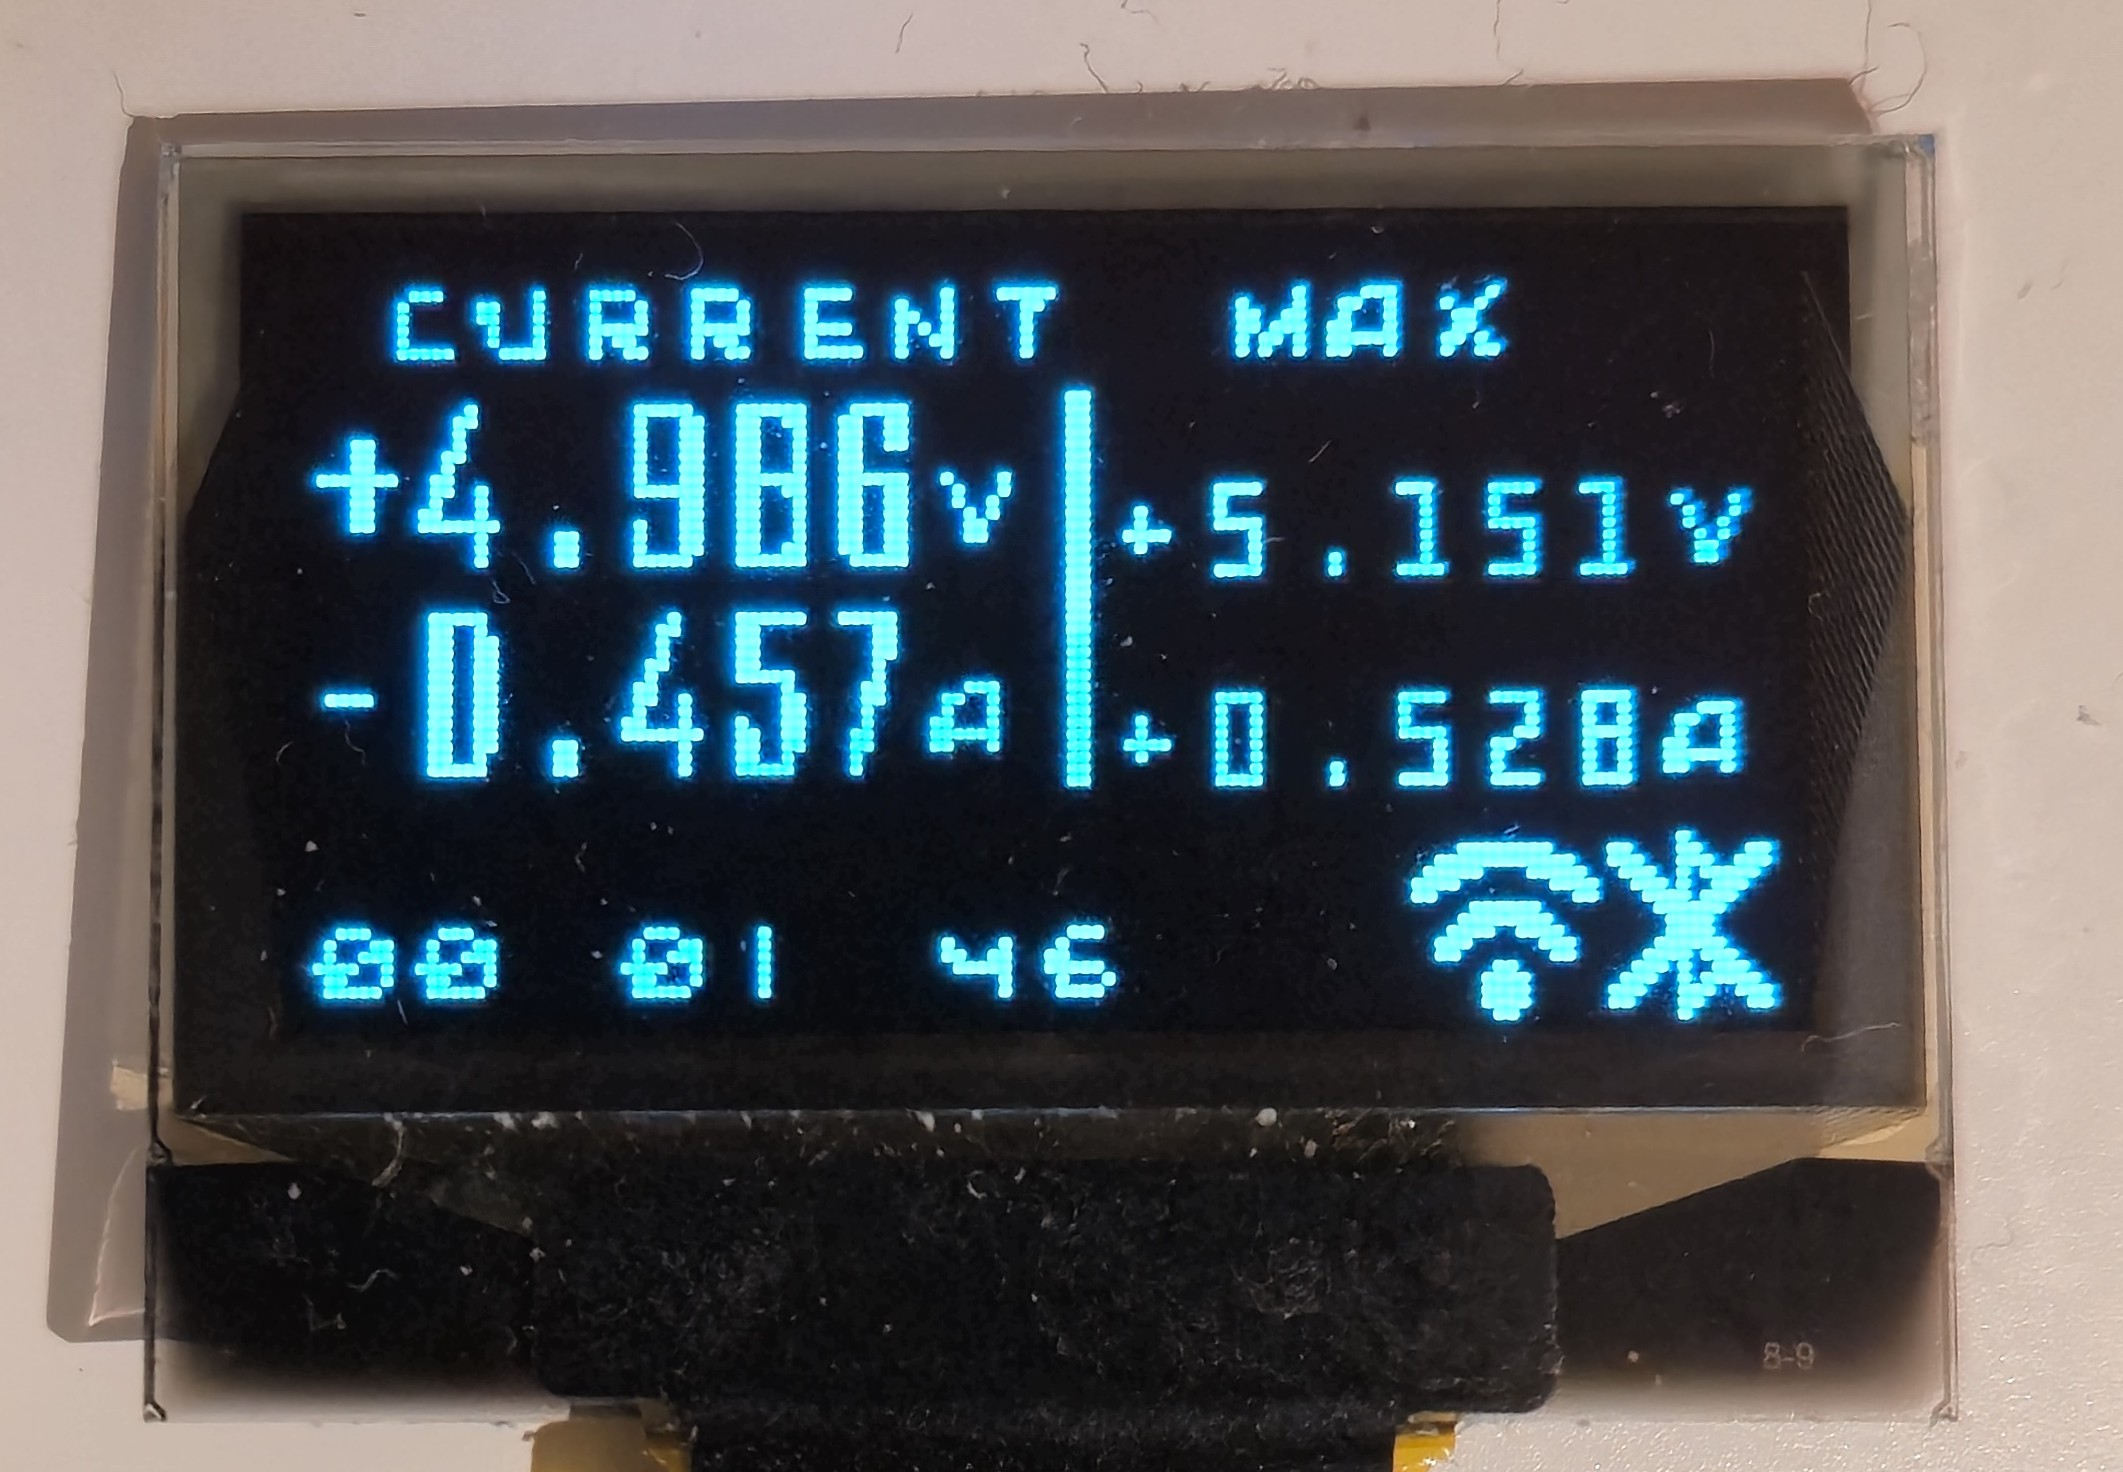
\includegraphics[width=\textwidth]{figures/3_FW_Figures/Page1.jpg}
		\end{minipage}
		\hspace{1.2cm}
		\begin{minipage}{0.30\textwidth}
			\centering
			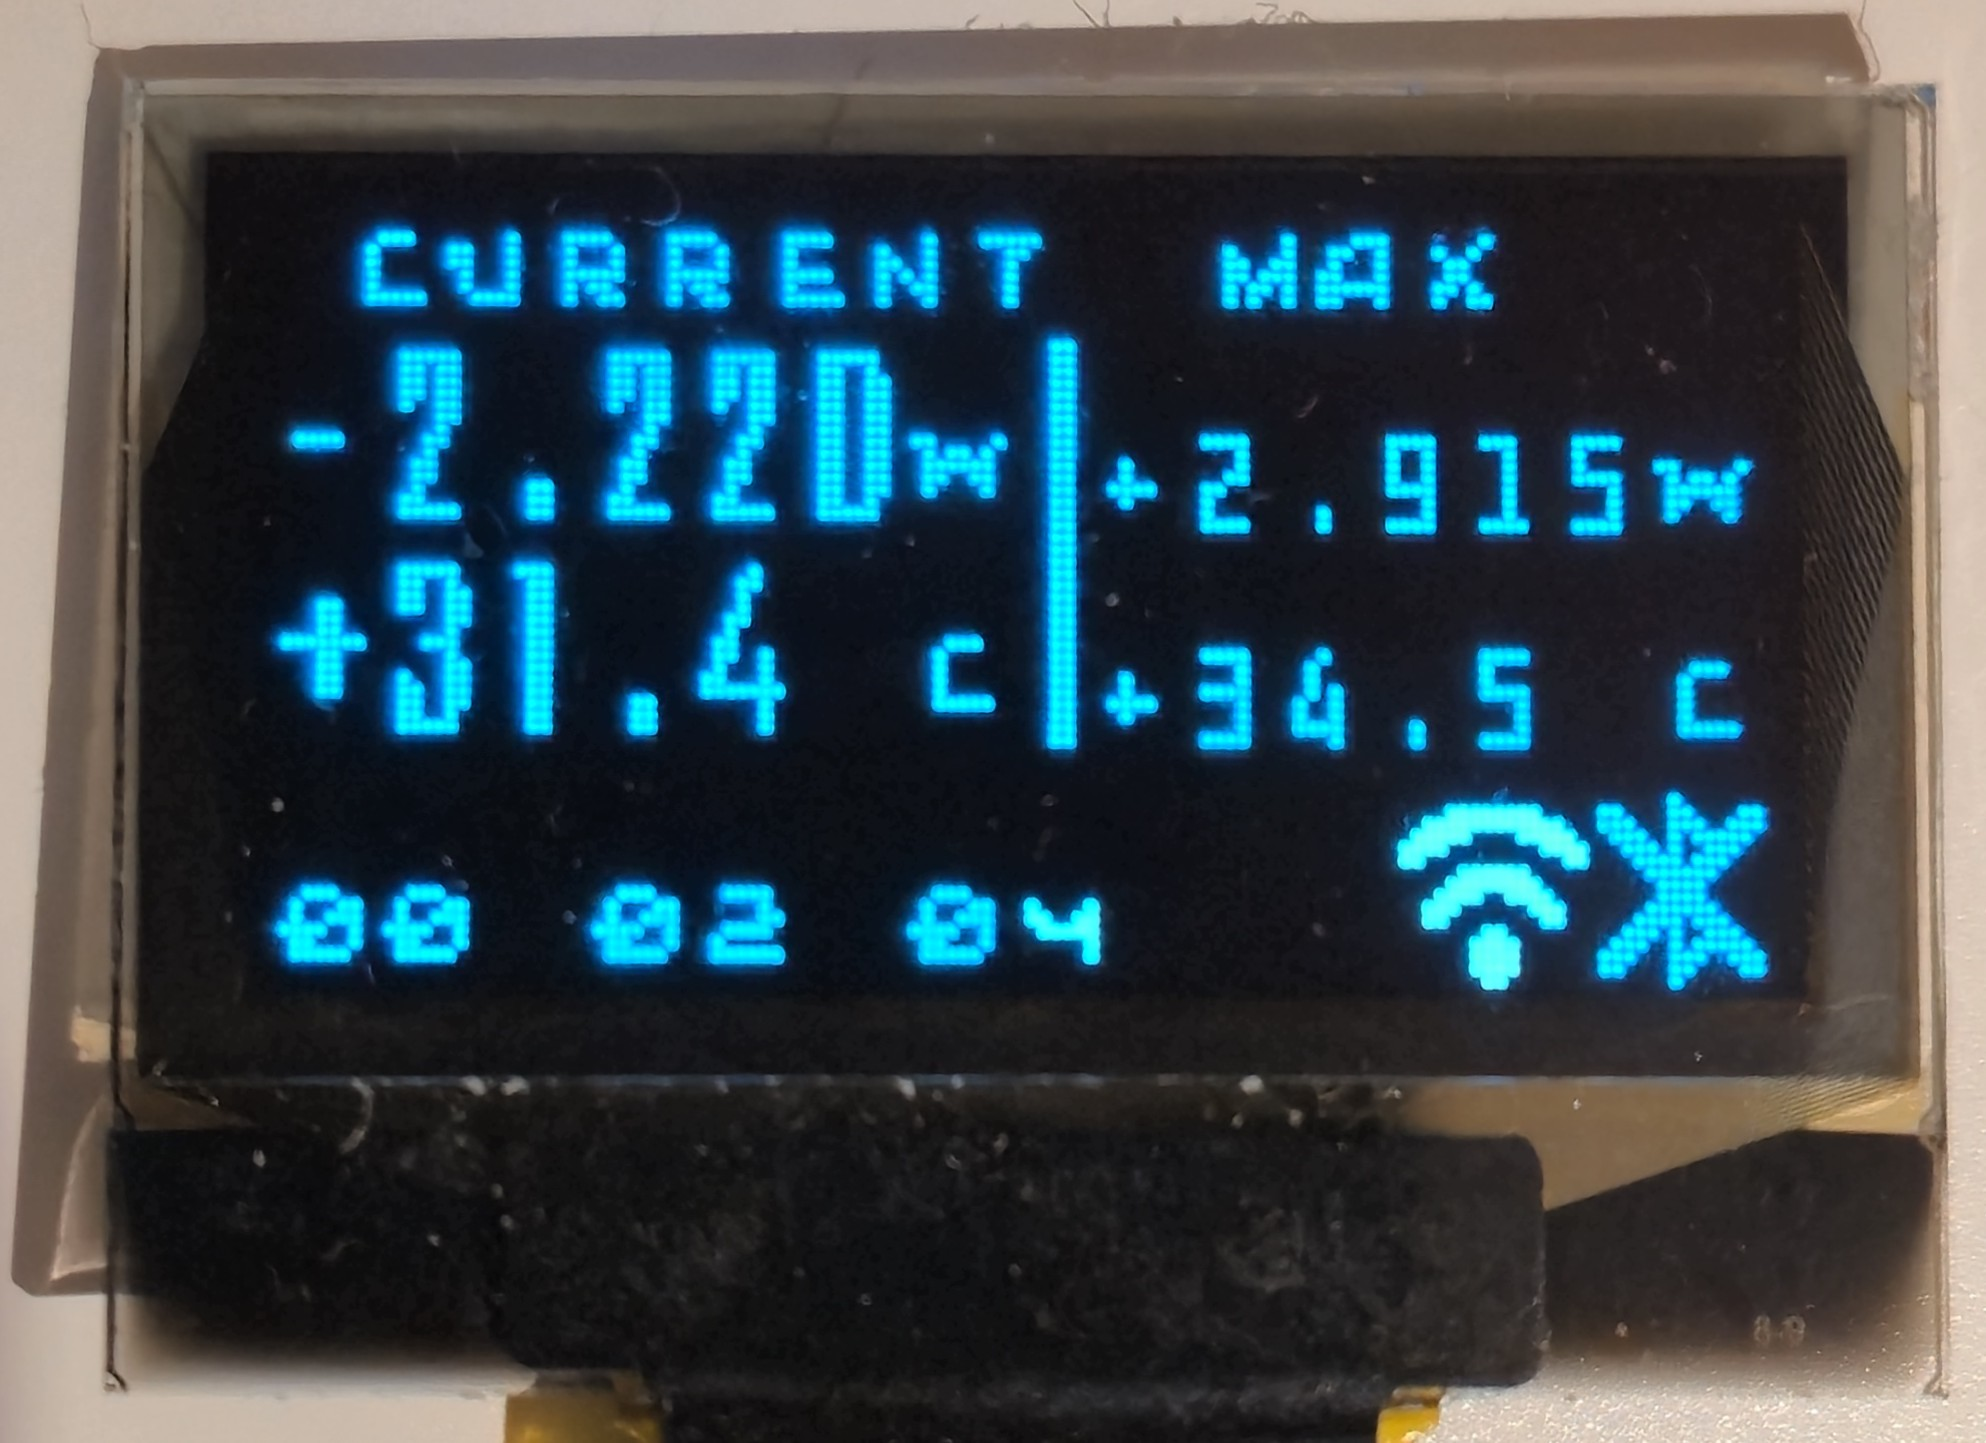
\includegraphics[width=\textwidth]{figures/3_FW_Figures/Page2.jpg}
		\end{minipage}
		
		\captionof{figure}{Live electrical measurement pages shown on the OLED display.}
		\label{fig:display_live_measurements}
		
	\end{center}

	
	\item \textbf{Energy page:} it shows the energy measured during the
	current charge or discharge session and the nominal battery energy configured
	through the BLE application.
	
	\begin{center}
		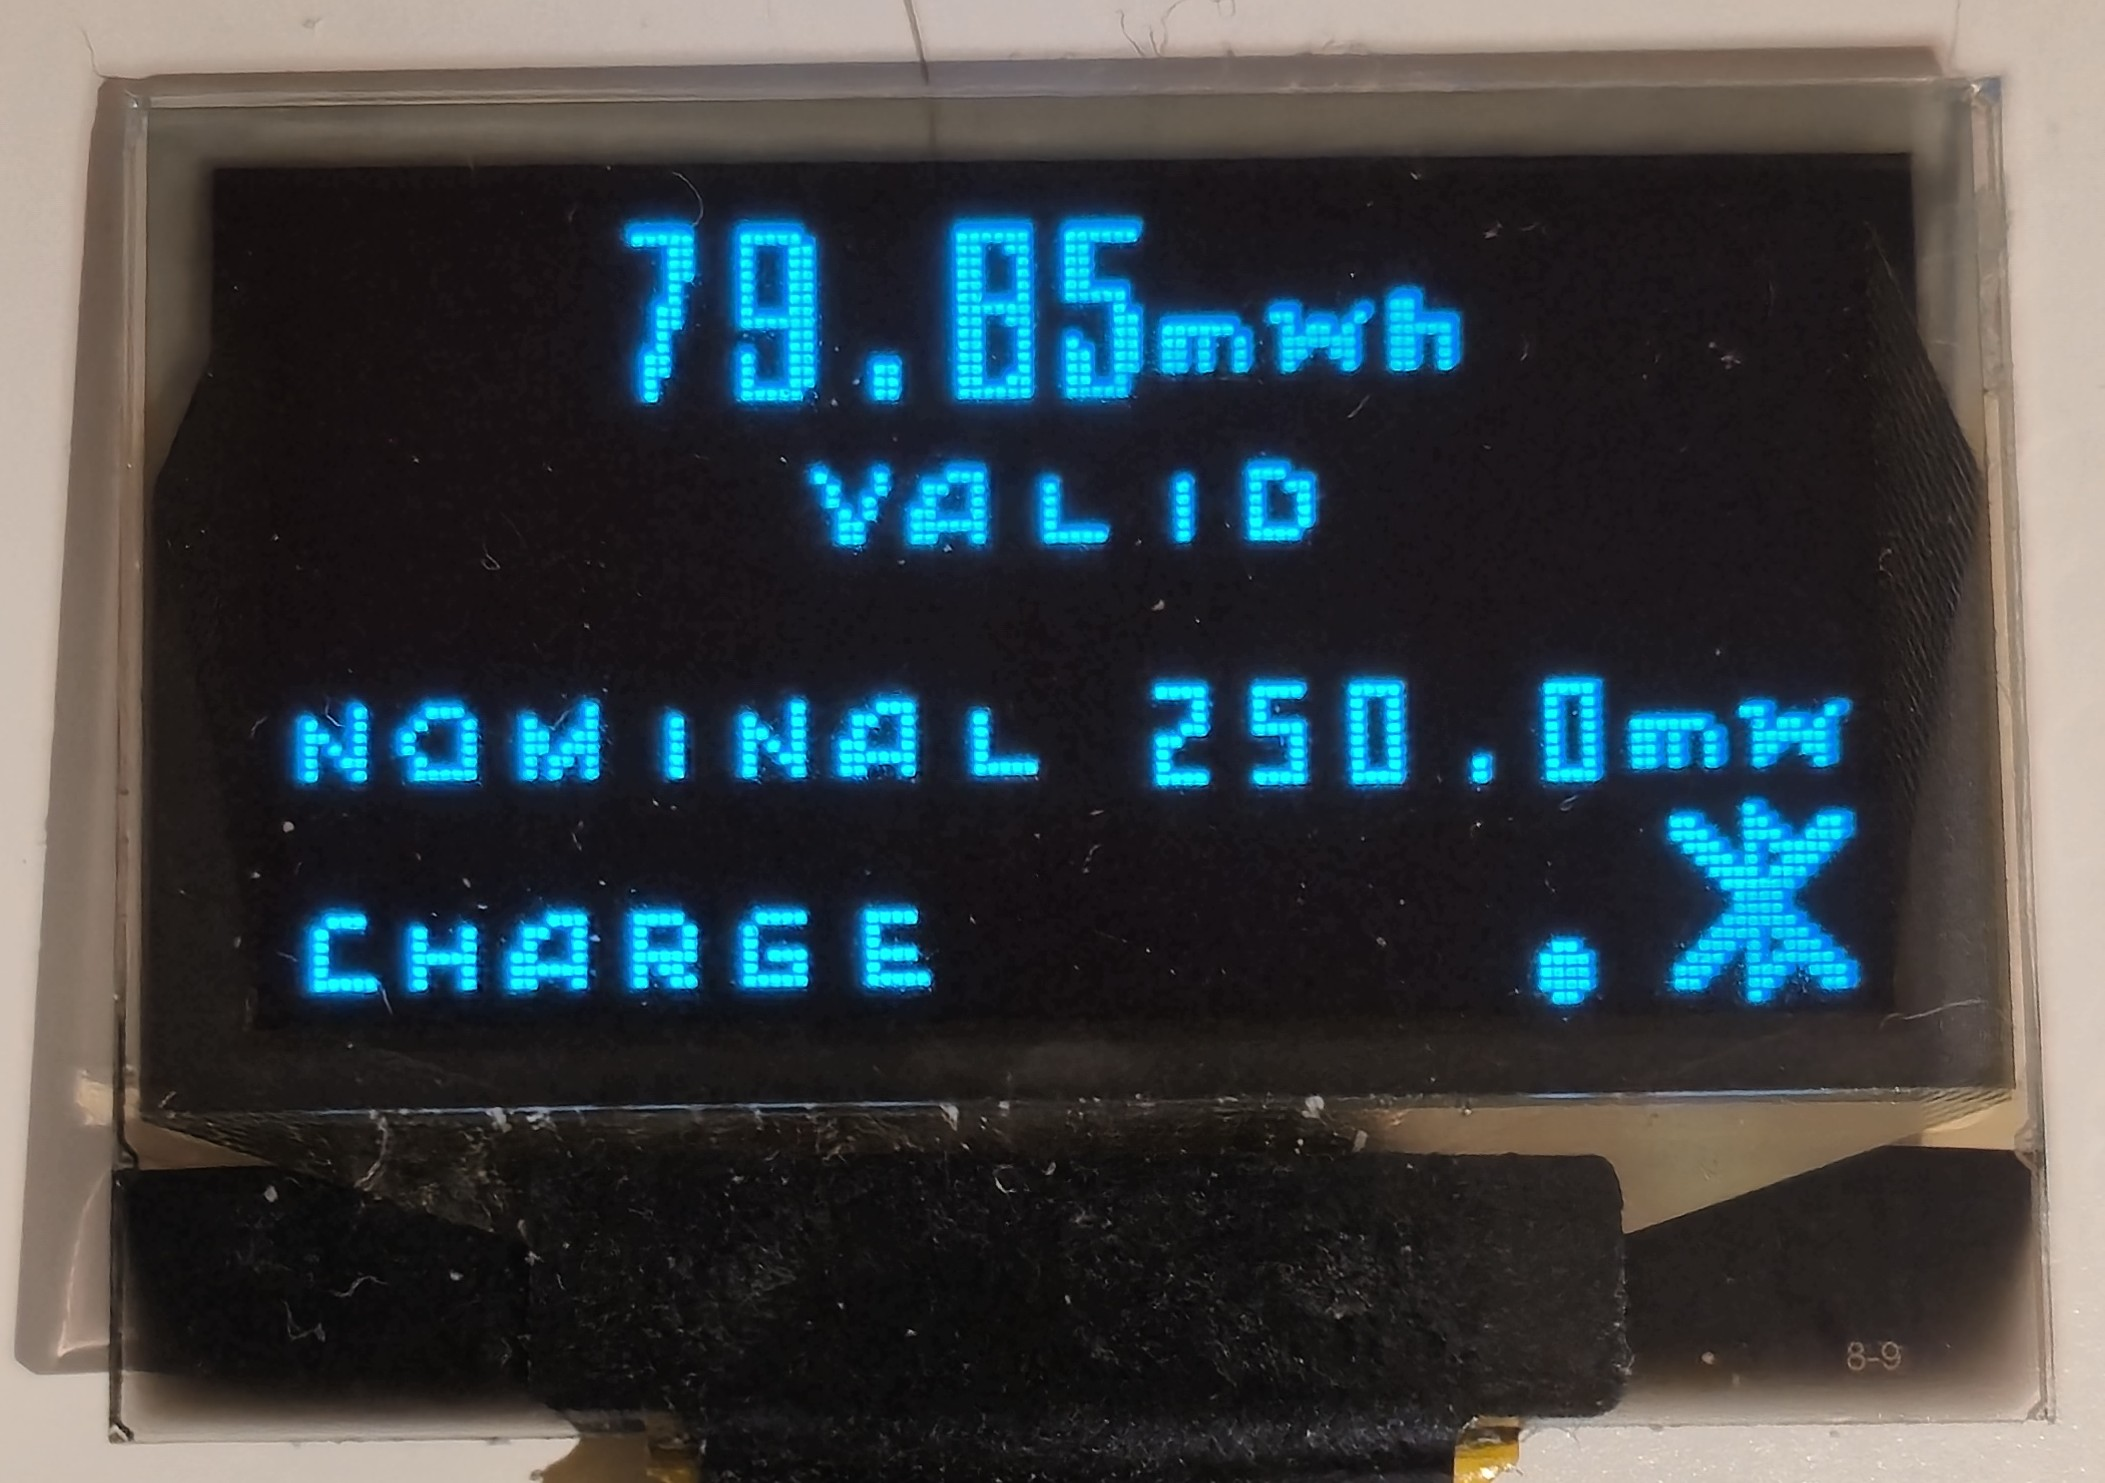
\includegraphics[width=0.30\textwidth]{figures/3_FW_Figures/Page3.jpg}
		\captionof{figure}{Energy page shown on the OLED display.}
		\label{fig:display_energy_page}
	\end{center}
	
	\item \textbf{State of Charge page:} it shows the estimated battery
	State of Charge (SoC), expressed as a percentage.
	
	\begin{center}
		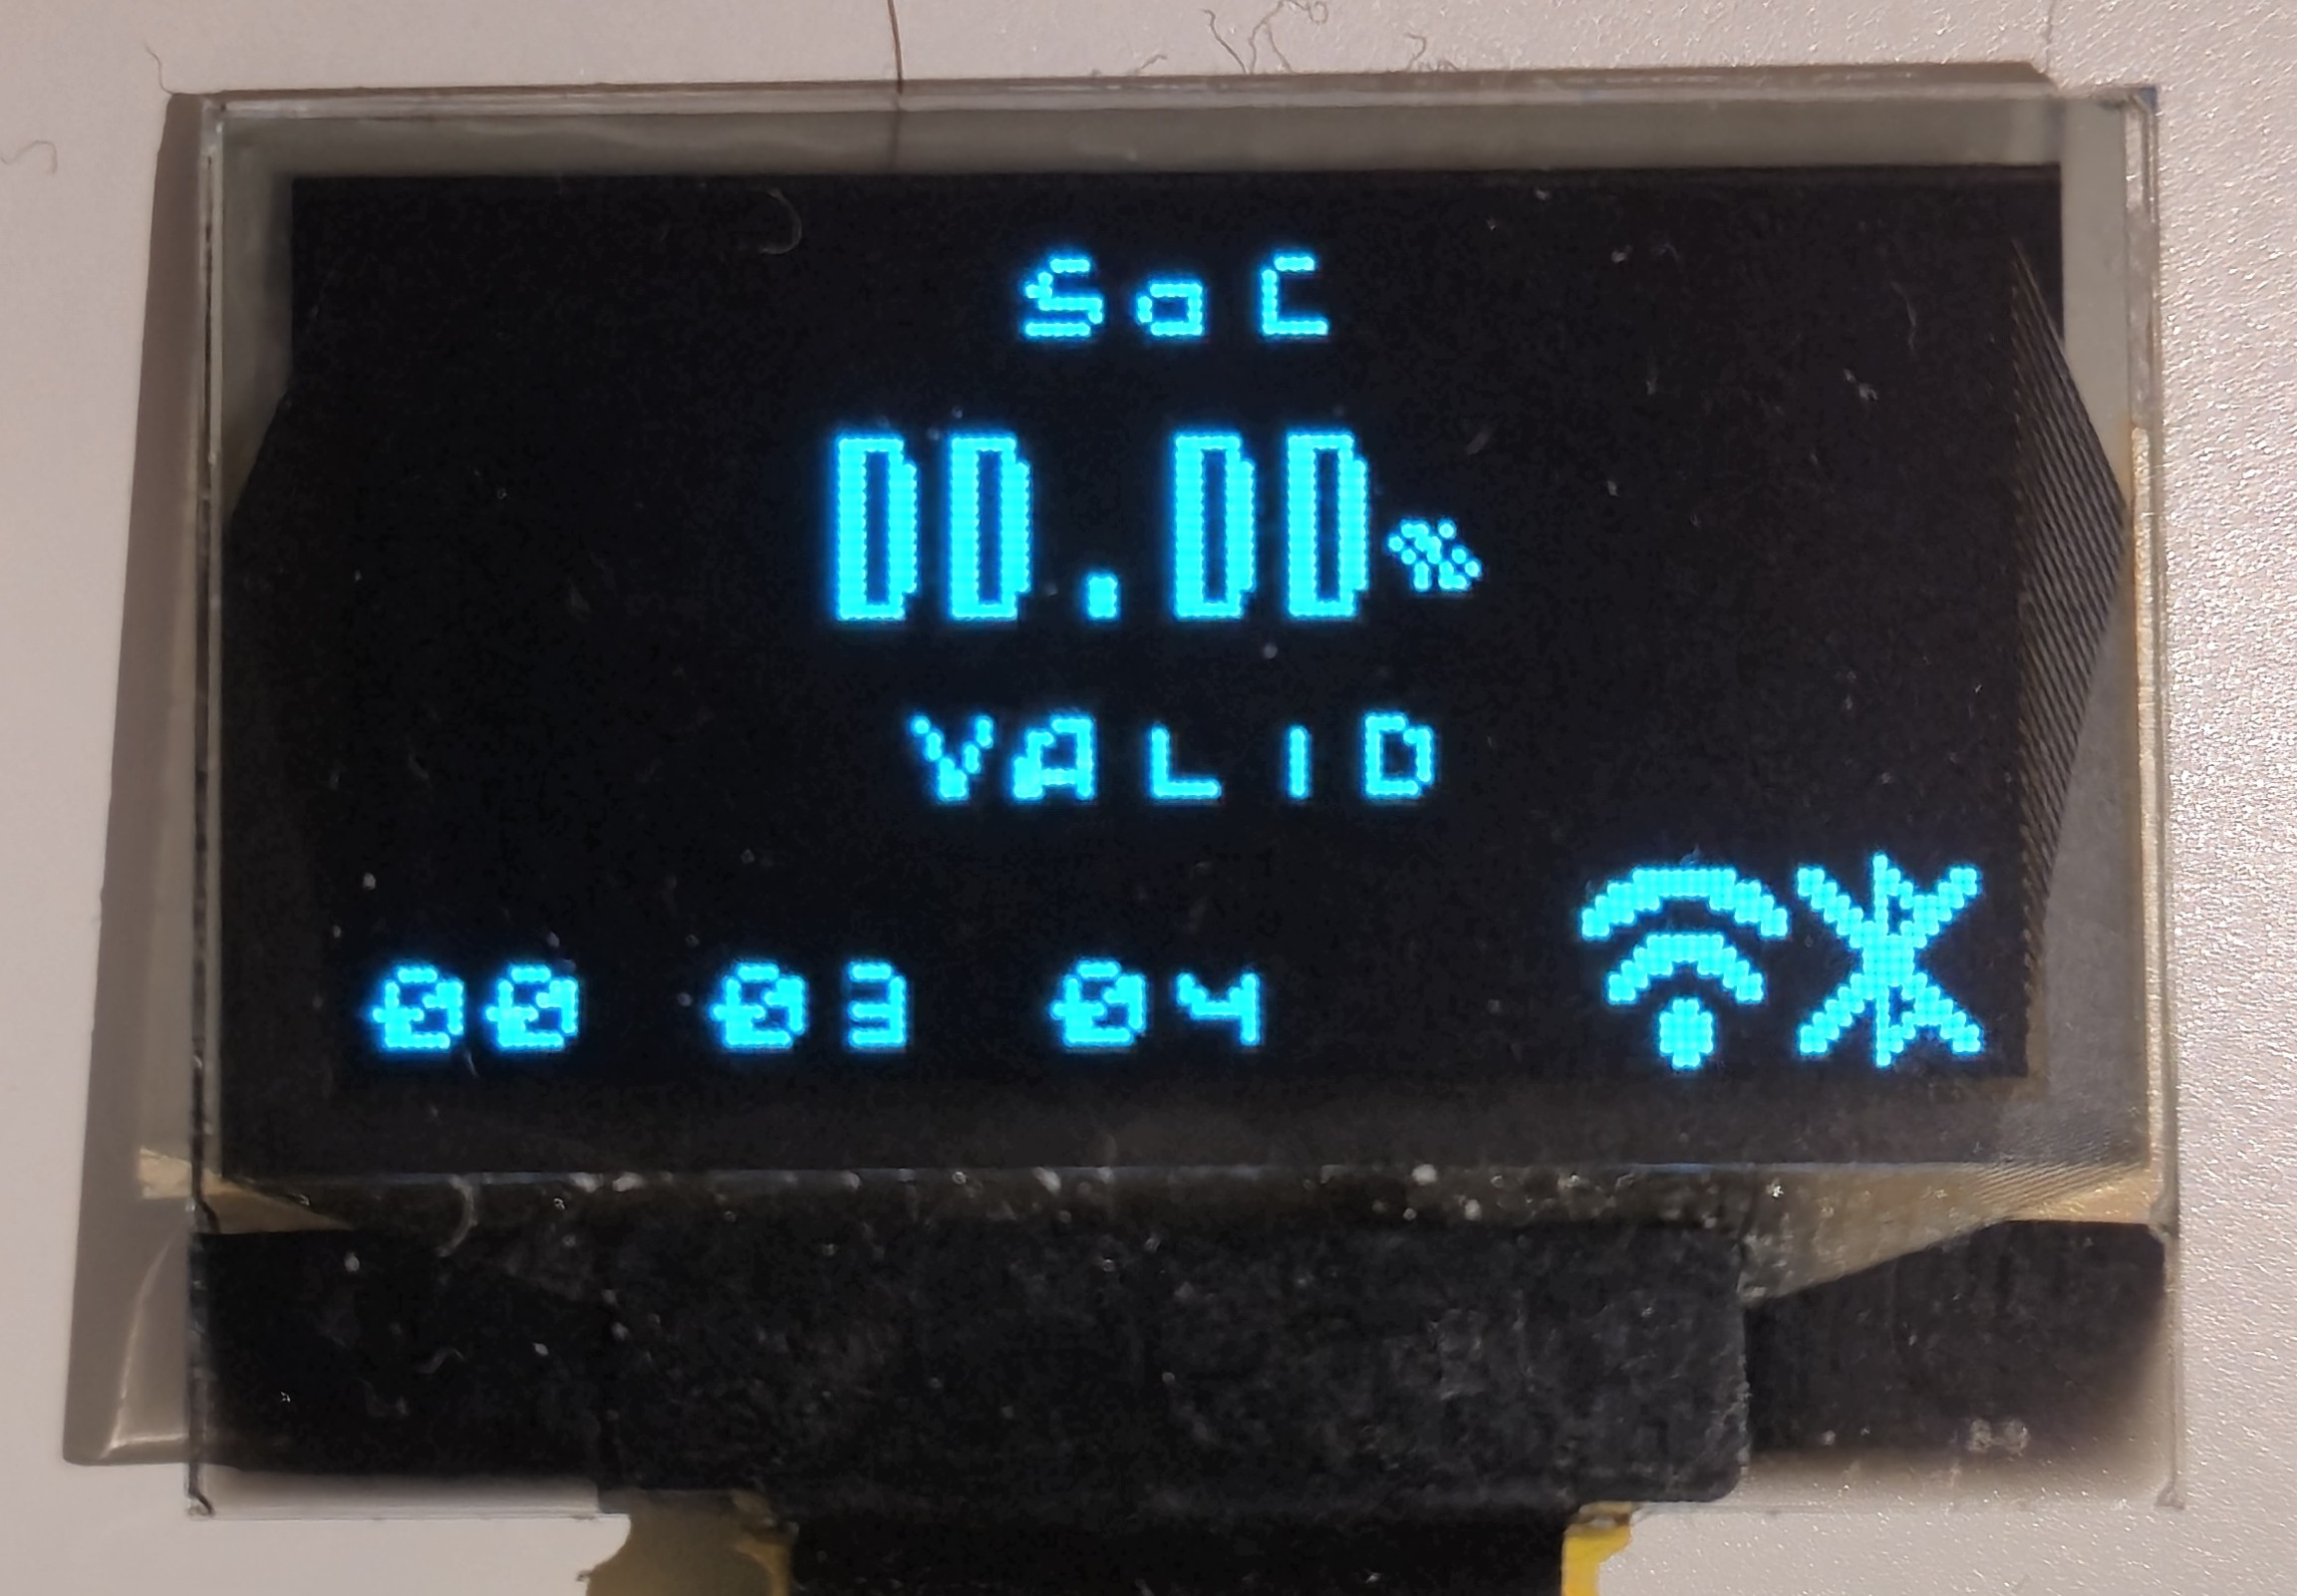
\includegraphics[width=0.30\textwidth]{figures/3_FW_Figures/Page4.jpg}
		\captionof{figure}{State of Charge page shown on the OLED display.}
		\label{fig:display_soc_page}
	\end{center}
	
	\item \textbf{State of Health page:} this page has the same structure as the
	SoC page, but it shows the estimated State of Health (SoH) of the battery.
	
	\begin{center}
		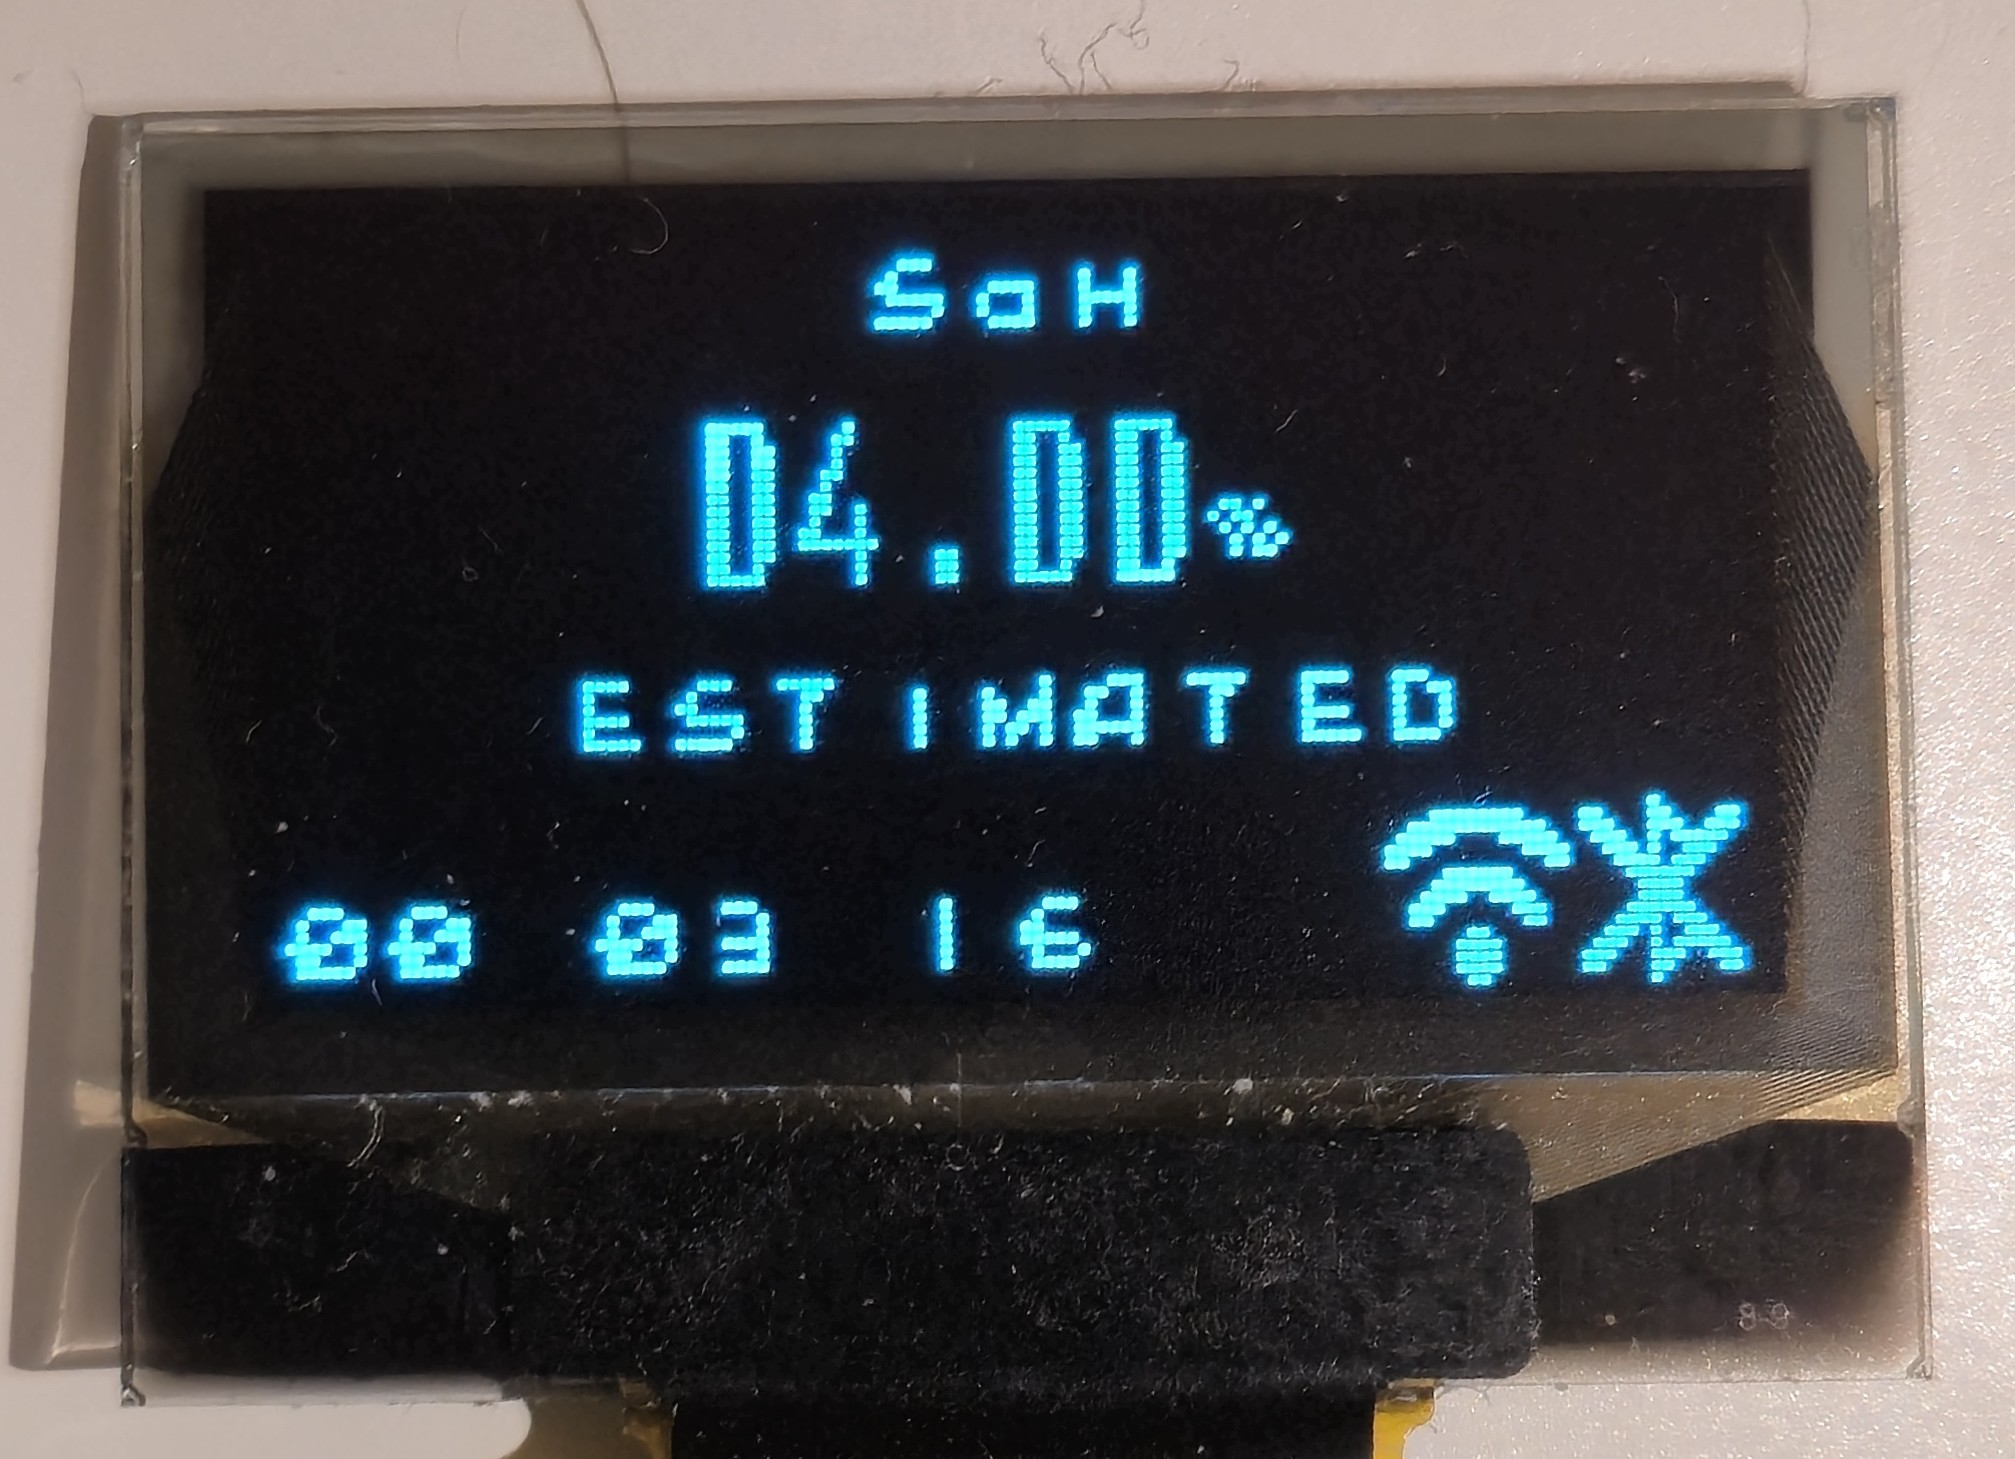
\includegraphics[width=0.30\textwidth]{figures/3_FW_Figures/Page5.jpg}
		\captionof{figure}{State of Health page shown on the OLED display.}
		\label{fig:display_soh_page}
	\end{center}
	
\end{itemize}


All measurements that depend on the previous history of the battery, namely the session energy, SoC and SoH, are accompanied by a tag that shows whether the corresponding value is \texttt{UNKNOWN}, \texttt{ESTIMATED} or \texttt{LEARNED}, as described in Section~\ref{Main_Application_Task}.

All normal pages include a compact footer region used to report secondary status information without affecting the main page content. Depending on the current operating condition, the footer can show either the active session time or the current session state.

The same footer region is also used to display BLE status information. The connection state is represented by a Bluetooth icon, while the link quality is shown through a compact signal indicator derived from the RSSI value provided by the BLE task. In this way, the user can check both the connection state and the approximate BLE signal quality in all avaiabe pages. The icon mapping and RSSI-based signal indication are summarized in Table~\ref{tab:ble_icon_display} and Table~\ref{tab:ble_signal_display}, respectively.

\begin{table}[H]
	\centering
	\small
	\caption{Bluetooth icons used by the OLED interface.}
	\label{tab:ble_icon_display}
	\begin{tabularx}{\textwidth}{
			@{}
			>{\raggedright\arraybackslash}X
			>{\raggedright\arraybackslash}X
			>{\centering\arraybackslash}m{1.6cm}
			@{}
		}
		\toprule
		\textbf{BLE connection state} &
		\textbf{Bluetooth icon} &
		\textbf{Symbol} \\
		\midrule
		
		Disconnected or advertising &
		Crossed Bluetooth icon &
		\tableicon{figures/NO_BLE_16x16.png} \\
		
		Connected &
		Bluetooth icon &
		\tableicon{figures/BLE_16x16.png} \\
		
		\bottomrule
	\end{tabularx}
\end{table}

\begin{table}[H]
	\centering
	\small
	\caption{BLE signal indicator selection based on connection state and RSSI.}
	\label{tab:ble_signal_display}
	\begin{tabularx}{\textwidth}{
			@{}
			>{\raggedright\arraybackslash}X
			>{\raggedright\arraybackslash}X
			>{\centering\arraybackslash}m{1.6cm}
			@{}
		}
		\toprule
		\textbf{BLE / RSSI state} &
		\textbf{Displayed signal indicator} &
		\textbf{Symbol} \\
		\midrule
		
		Idle, not connected and not advertising &
		Hidden &
		-- \\
		
		Advertising &
		Animated search indicator &
		-- \\
		
		Connected, RSSI $< -75$ dBm &
		Hidden &
		-- \\
		
		Connected, $-75 \leq \mathrm{RSSI} < -60$ dBm &
		Low signal indicator &
		\tableicon{figures/BLE_anim2.png} \\
		
		Connected, $-60 \leq \mathrm{RSSI} < -45$ dBm &
		Medium signal indicator &
		\tableicon{figures/BLE_anim3.png} \\
		
		Connected, $\mathrm{RSSI} \geq -45$ dBm &
		Strong signal indicator &
		\tableicon{figures/BLE_anim4.png} \\
		
		\bottomrule
	\end{tabularx}
\end{table}

\paragraph{Warning overlay.}
Safety warnings are not implemented as a separate display page. Instead, when a danger condition is active, the Display task draws a warning banner on top of the currently selected page. This makes the warning visible independently of the page currently selected by the user. The danger state is still computed by the App task, while the Display task only renders the corresponding visual indication.

\begin{center}
	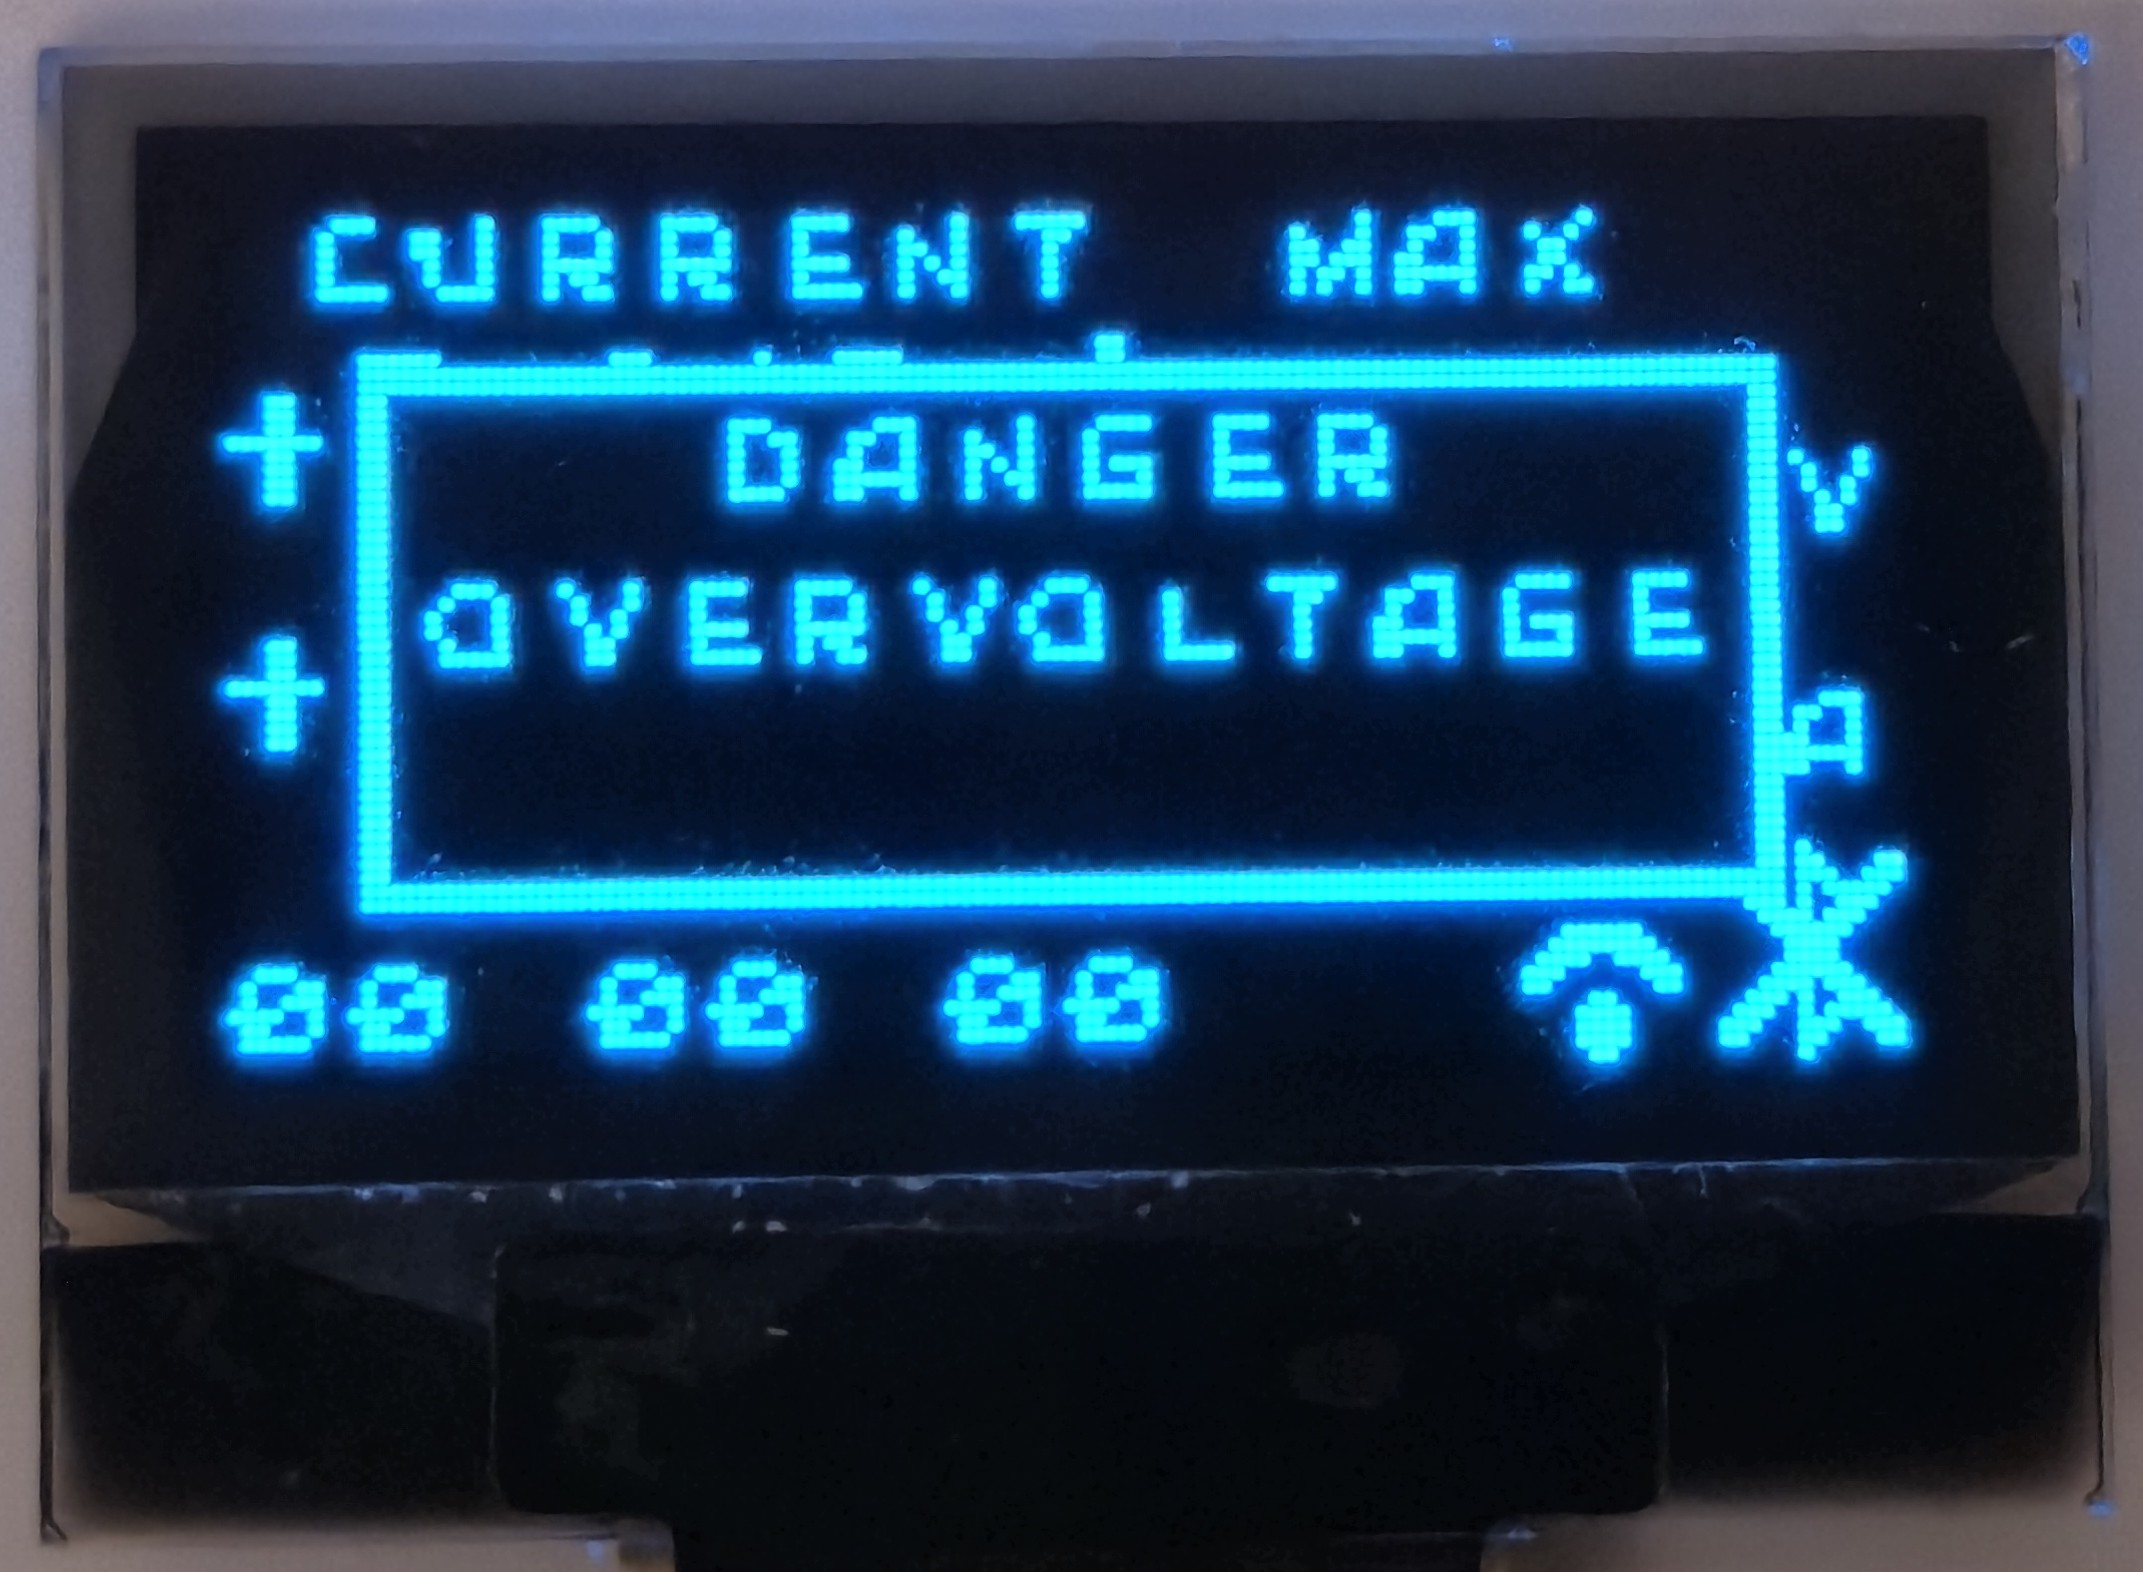
\includegraphics[width=0.30\textwidth]{figures/3_FW_Figures/Page7.jpg}
	\captionof{figure}{Energy page shown on the OLED display.}
	\label{fig:display_danger}
\end{center}

\subsection{Flash Storage Application Task}

The Flash Storage task provides the non-volatile storage backend for the battery estimation state. It is implemented as a separate RTOS task because flash program and erase operations are slower and more restrictive than normal RAM accesses. The App task does not access the flash driver directly; instead, it posts high-level storage requests to the Flash Storage mailbox, while the Flash Storage task performs the required low-level operations.

Although the amount of data to be preserved is small, the firmware uses one available flash page as an append-only log. This avoids treating flash as a directly overwritten variable and reduces the number of page erase operations required during normal operation.

\paragraph{Stored records.}
The flash page is shared by two record classes, selected according to their update rate. Fast checkpoint records are written periodically during active charge or discharge sessions and are used to recover the current session after an unexpected reset. Slow records are written only when long-term battery information changes, such as the configured nominal energy or the last completed cycle energy.

Keeping both record types in the same flash page avoids reserving separate pages for small amounts of data. The available space is instead split according to the expected write rate of each record type, assigning most of the page to frequent checkpoints and a smaller area to slow records.

\begin{table}[H]
	\centering
	\small
	\caption{Flash record types used by the Flash Storage task.}
	\label{tab:flash_record_types}
	\begin{tabularx}{\textwidth}{l l X}
		\toprule
		\textbf{Record type} & \textbf{Size} & \textbf{Stored information} \\
		\midrule
		Fast checkpoint &
		8 bytes &
		Sequence counter, current cycle energy, flags, and CRC. \\
		
		Slow record &
		16 bytes &
		Nominal battery energy, last completed cycle energy, completed cycle count, last completed session state, flags, and CRC. \\
		\bottomrule
	\end{tabularx}
\end{table}

Fast checkpoints allow the firmware to recover the current session energy if the device resets during a charge or discharge cycle. Slow records preserve longer-term information, such as the configured nominal energy and the last learned cycle energy used for SoC and SoH estimation.

\paragraph{Append-only storage and recovery.}
Flash memory cannot be overwritten freely: bits can be programmed from \(1\) to \(0\), but returning them to \(1\) requires erasing the whole flash page. For this reason, each new record is written in the next empty slot of its corresponding area. When the available slots are exhausted, the page is erased and the latest record that must be preserved is written again after the erase.

At startup, the Flash Storage task scans the reserved page to reconstruct the last stored state. Empty records are ignored, while programmed records are decoded and ordered using their sequence counter. The newest valid record is then selected as the current non-volatile state. This allows the firmware to recover the latest stored information without overwriting previous records in place.

\paragraph{Flash page allocation and endurance.}
The reserved flash page has a size of \(B_{page} = 4096\,\mathrm{B}\). The split between fast and slow records is computed from the expected write periods and record sizes:

\begin{itemize}
	\item fast checkpoint period: \(T_f = 30\,\mathrm{s}\);
	\item average slow record period: \(T_s = 3600\,\mathrm{s}\);
	\item fast record size: \(S_f = 8\,\mathrm{B}\);
	\item slow record size: \(S_s = 16\,\mathrm{B}\).
\end{itemize}

The amount of flash reserved for slow records is selected so that the fast and slow areas are consumed at approximately the same rate. The ideal value is then rounded to an integer number of slow records:

\[
B_s^\star =
\frac{B_{page} \cdot T_f \cdot S_s}
{T_f \cdot S_s + T_s \cdot S_f}
=
\frac{4096 \cdot 30 \cdot 16}
{30 \cdot 16 + 3600 \cdot 8}
\approx
67\,\mathrm{B}
\xrightarrow{B_s = 64\,\mathrm{B}}
\left\{
\begin{aligned}
	N_s &= \frac{B_s}{S_s} = \frac{64}{16} = 4 \\
	N_f &= \frac{B_{page} - B_s}{S_f} = \frac{4096 - 64}{8} = 504
\end{aligned}
\right.
\]

The resulting allocation provides \(4\) slow records and \(504\) fast checkpoints in one flash page. With one checkpoint every \(30\,\mathrm{s}\), the fast area covers:

\[
T_{page,f} =
N_f \cdot T_f
=
504 \cdot 30\,\mathrm{s}
=
15120\,\mathrm{s}
\approx
4.2\,\mathrm{h}
\]

A similar calculation can be performed for the slow area, which provides approximately \(4\,\mathrm{h}\) of operation before the slow-record slots are exhausted. Therefore, the two areas are consumed at approximately the same rate.

Therefore, the two areas are consumed at approximately the same rate.

Considering a flash endurance of \(100000\) erase cycles, the theoretical active-session endurance is:

\[
T_{\mathrm{active,max}} =
100000 \cdot T_{page,f}
=
100000 \cdot 504 \cdot 30\,\mathrm{s}
=
1.512 \cdot 10^9\,\mathrm{s}
=
420000\,\mathrm{h}
\approx
47.9\,\mathrm{years}
\]

This value represents the theoretical lifetime during charge or discharge activity. Periods in which WattMate is powered on, but no power is transmitted on the USB bus is not counted in this computation, because in that case no new record is saved on Flash Memory.

\paragraph{Data integrity.}
Each record contains a CRC field. After programming a record, the Flash Storage task reads it back and decodes it again before updating the in-RAM storage state. During startup scanning, records with an invalid CRC are discarded. This prevents partially written or corrupted records from being used as valid battery state.


\subsection{Input Application Task}
\label{sec:input_task}

The Input task manages the physical inputs of WattMate and converts low-level hardware events into application-level events. Its role is intentionally limited: it does not decide the system behavior, but it detects user actions, PAC alert signals, and temperature samples, then immediately notifies the App task.

\paragraph{User button handling.}
The user button is handled through GPIO interrupts and RTOS timers. When an edge is detected, the button interrupt is temporarily disabled and a debounce timer is started. The debounce time is set to \(30\,\mathrm{ms}\). After this interval, the button level is sampled again and the task decides whether a valid press or release occurred.

A second timer is used for long-press detection. If the button remains active for \(800\,\mathrm{ms}\), the Input task posts a long-press event to the App task. Otherwise, when the button is released before the long-press timeout, a normal button-press event is generated. This allows the App task to receive clean user events without directly handling mechanical bouncing or button timing.

\paragraph{PAC alert inputs.}
The PAC1951 alert pins are also managed by the Input task. These pins are configured as interrupt sources and are used to notify the App task when a hardware alert occurs. In this way, configured PAC1951 alert conditions can be forwarded immediately to the App task, without waiting for the next standard I2C communication cycle.

\paragraph{Temperature sampling.}
The NTC temperature measurement is controlled by the Input task through the ADC driver. Sampling is not always active: the App task enables the temperature measuremnets according to the current runtime needs commanded by the App task, for example when the display is showing temperature information or when BLE telemetry is active.

When temperature sampling is enabled, the Input task performs one sample every \(200\,\mathrm{ms}\). For each sample, the task enables the NTC divider, waits \(5\,\mathrm{ms}\) to let the analog node settle, and then performs the ADC conversion. 

The raw ADC value is converted into centi-degrees Celsius using a precomputed NTC lookup table. The table is generated offline from the NTC beta model, using

\[
R_{NTC}(T) =
R_0 e^{B\left(\frac{1}{T_K} - \frac{1}{T_0}\right)}
\]

where \(R_0 = 10\,\mathrm{k\Omega}\), \(T_0 = 298.15\,\mathrm{K}\), and
\(B = 3435\,\mathrm{K}\). Given the hardware NTC circuit, the expected ADC code
for each temperature is computed as

\[
ADC_{LUT}(T) =
ADC_{max}
\frac{V_{DD}}{V_{FS}}
\frac{R_{NTC}(T)}{R_1 + R_{NTC}(T)}.
\]

In the current firmware, the LUT is generated assuming \(V_{DD}=3.3\,\mathrm{V}\). However, the real board supply voltage is provided by the DC/DC converter and can be slightly different from this nominal value. Since the ADC code depends on the voltage applied to the NTC circuit, using the raw ADC value directly would introduce a temperature error whenever the real supply voltage differs from \(3.3\,\mathrm{V}\).

For this reason, before accessing the lookup table, the firmware reads the actual board supply voltage using the internal battery monitor of the MCU and rescales the measured ADC code to the equivalent value that would have been measured with the nominal LUT supply voltage:

\[
ADC_{scaled} =
ADC_{raw}
\frac{V_{DD,LUT}}{V_{DD,meas}}.
\]

The lookup table is then searched using \(ADC_{scaled}\), not the uncorrected raw ADC value. Since the LUT contains discrete points, the final temperature is obtained by linear interpolation between the two adjacent table entries. If

\[
ADC_i \geq ADC_{scaled} \geq ADC_{i+1},
\]

the temperature is computed as

\[
T =
T_i +
\frac{ADC_i - ADC_{scaled}}{ADC_i - ADC_{i+1}}
\left(T_{i+1} - T_i\right).
\]

The resulting value is stored in centi-degrees Celsius. This approach avoids evaluating the full NTC equation at runtime, while still compensating for supply-voltage variations of the board.



\subsection{PAC Application Task}
\label{PAC_Application_Task}

The PAC1951 Application task manages the interface between WattMate and the PAC1951 power monitor. Its role is to configure the sensor, select the appropriate sampling profile, control when I2C measurement reads are performed, and publish electrical measurement snapshots to the App task.

The task is separated from the main App task because the PAC1951 is not only a measurement device. It also provides hardware alert outputs, internal sampling configuration, programmable thresholds, and an energy accumulator. Keeping these details inside the PAC task allows the App task to request high-level sensor actions without directly handling the PAC1951 driver configuration.

The App task interacts with the PAC task through high-level commands posted to its RTOS mailbox. These commands do not directly access the PAC1951 driver; they only request sensor-level actions. The detailed execution is handled internally by the PAC task. The main command categories are summarized in Table~\ref{tab:pac_task_commands}.

\begin{table}[H]
	\centering
	\small
	\caption{Main command categories handled by the PAC task.}
	\label{tab:pac_task_commands}
	\begin{tabularx}{\textwidth}{lX}
		\toprule
		\textbf{Command category} & \textbf{Purpose} \\
		\midrule
		Profile control & Switch the PAC1951 between idle and normal sampling profiles. \\
		Measurement stream control & Enable or disable periodic I2C reads from the PAC1951. \\
		Accumulator read control & Enable or disable PAC1951 accumulator reads. \\
		\bottomrule
	\end{tabularx}
\end{table}

\paragraph{PAC1951 configuration.}
The PAC1951 is configured as the main electrical measurement device of WattMate. The bus-voltage measurement is configured as unipolar, while the sense-current measurement is configured as bipolar, allowing the firmware to represent both charge and discharge current directions.

The accumulator is configured in power accumulation mode. This allows the accumulated quantity to be directly converted into energy over time. When energy measurement is enabled, the PAC task reads the accumulator contribution, adds it to the current session energy counter, and publishes the updated energy value together with the live electrical snapshot.

\begin{table}[H]
	\centering
	\small
	\caption{Main PAC1951 measurement configuration.}
	\label{tab:pac_measurement_configuration}
	\begin{tabularx}{\textwidth}{lX}
		\toprule
		\textbf{Measurement} & \textbf{PAC1951 configuration} \\
		\midrule
		Bus voltage & Channel 1 bus-voltage measurement, configured as unipolar. \\
		Sense current & Channel 1 sense-voltage measurement, configured as bipolar and converted using a \(10\,\mathrm{m\Omega}\) sense resistor. \\
		Power & Computed by the PAC1951 from bus voltage and sense current. \\
		Energy & Obtained by configuring the PAC1951 accumulator in power accumulation mode. \\
		\bottomrule
	\end{tabularx}
\end{table}

\paragraph{Sampling profiles.}
The PAC task defines two sampling profiles. Each profile represents a complete PAC1951 operating configuration, including sampling mode, alert routing, thresholds, and alert sample counts. The profiles used by WattMate are summarized in Table~\ref{tab:pac_sampling_profiles}.

\begin{table}[H]
	\centering
	\small
	\caption{PAC1951 sampling profiles used by WattMate.}
	\label{tab:pac_sampling_profiles}
	\begin{tabularx}{\textwidth}{lXX}
		\toprule
		\textbf{Parameter} & \textbf{Idle profile} & \textbf{Normal profile} \\
		\midrule
		Sampling mode &
		\(8\) samples/s, adaptive accumulation mode &
		\(64\) samples/s, adaptive accumulation mode \\
		
		Main purpose &
		Bus activity detection with reduced sampling activity &
		Active charge/discharge measurement and safety supervision \\
		
		\texttt{ALERT1} routing &
		Electrical safety detection &
		Electrical safety detection \\
		
		\texttt{ALERT2} routing &
		Over-power event used as wake-up source &
		Accumulator-fullness indication \\
		
		Over-power threshold &
		\(50\,\mathrm{mW}\) &
		Not used for wake-up \\
		
		Safety thresholds &
		\(30000\,\mathrm{mV}\) overvoltage,
		\(5000\,\mathrm{mA}\) overcurrent &
		\(30000\,\mathrm{mV}\) overvoltage,
		\(5000\,\mathrm{mA}\) overcurrent \\
		
		Safety alert sample count &
		\(4\) samples &
		\(4\) samples \\
		
		Wake-up alert sample count &
		\(1\) sample &
		Not used \\
		\bottomrule
	\end{tabularx}
\end{table}

The idle profile is used when no active charge or discharge session is present. In this mode, the PAC1951 is not shut down completely, but continues to monitor the power bus at a reduced sampling rate. This allows the MCU to remain in a low-power state while the PAC1951 autonomously detects relevant bus activity.

This approach avoids periodic one-shot measurements initiated by the MCU. Instead, \texttt{ALERT2} is configured as a wake-up source when the absolute bus power exceeds the session start threshold, equal to \(50\,\mathrm{mW}\). Safety supervision remains active through \texttt{ALERT1}, so overvoltage and overcurrent conditions can still be reported while the system is idle.

The normal profile is used during active charge or discharge sessions. In this mode, the PAC1951 operates at a higher sampling rate to support energy accumulation and real-time supervision. \texttt{ALERT1} remains assigned to electrical safety events, while \texttt{ALERT2} is reconfigured as an accumulator-fullness indication, allowing the firmware to read accumulated measurements when new data are available.

\paragraph{Measurement stream.}
The PAC1951 sampling profile and the MCU measurement stream are intentionally kept separate. The sampling profile defines how the sensor operates internally, while the measurement stream defines whether the MCU periodically reads the latest values through I2C.

When the stream is requested, the PAC task performs an immediate read and then uses an RTOS clock to schedule the following reads according to the active PAC sampling mode. When the stream is released, the clock is stopped and no periodic I2C transactions are performed, even if the PAC1951 remains configured and active.

This separation supports power management. The PAC1951 can continue monitoring the bus with the selected profile, while the MCU avoids unnecessary I2C transactions whenever live measurements are not required by the App task, the display, or the BLE interface.


\subsection{WattMate BLE Application Task}

The WattMate BLE Application task manages the wireless interface of WattMate. Its role is to isolate the BLE stack, the GATT service, advertising, connection events and notification timing from the rest of the firmware. The App task does not call the BLE stack directly; instead, it interacts with the BLE task through high-level commands.

This separation is useful because BLE communication has its own asynchronous execution model. Connection events, characteristic writes, notification availability and RSSI updates are generated by the BLE stack, while the rest of the firmware only needs to know whether the device is connected, whether the mobile application requested streaming, and when BLE data must be published.

\begin{table}[H]
	\centering
	\small
	\caption{Main command categories handled by the WattMate BLE task.}
	\label{tab:ble_task_commands}
	\begin{tabularx}{\textwidth}{lX}
		\toprule
		\textbf{Command category} & \textbf{Purpose} \\
		\midrule
		Advertising control 		& Start or stop BLE advertising and select the advertising profile. \\
		Stream control 				& Enable or disable periodic BLE notifications. \\
		Connection configuration	& Configure BLE transmission power and connection timing parameters. \\
		GATT event handling			& Process characteristic writes and notify the App task when the mobile application changes a setting. \\
		RSSI monitoring				& Periodically read the connection RSSI and make it available to the App and Display tasks. \\
		\bottomrule
	\end{tabularx}
\end{table}

\paragraph{GATT interface handling.} The BLE task registers and manages the custom GATT service specified in Section~\ref{sec:wattmate_custom_gatt_service} and summarized in Table~\ref{tab:wattmate_gatt_characteristics}. It handles characteristic writes, notification configuration changes, and notification requests, but it does not define the application meaning of the received commands by itself. For example, a write to the Control characteristic, whose payload is specified in Table~\ref{tab:wattmate_control_payload}, is converted into an application event, while the App task decides how the system state must change.

\paragraph{Advertising and connection state.}
The BLE task controls when WattMate is discoverable and selects the active advertising profile according to the current application state. 
The externally visible advertising payload and timing values are reported in Section~\ref{sec:wattmate_advertising_data}, Table~\ref{tab:wattmate_advertising_profiles}, and Figure~\ref{fig:wattmate_advertising_timing}.

When a central device connects, the BLE task updates its internal connection state and notifies the App task. 
When the connection is lost, the stream is stopped, the RSSI value is invalidated, and the App task is informed so that the system can return to the appropriate advertising state.

\paragraph{Telemetry streaming.}
BLE notifications are sent only when a connection is active, the mobile application has enabled the required notification descriptors, and the telemetry stream has been enabled. 
The externally visible notification timing is reported in Section~\ref{sec:wattmate_streaming_timing} and Figure~\ref{fig:wattmate_streaming_timing}.

At each stream update, the BLE task reads the latest application snapshot and packs it into the corresponding GATT payloads. 
The BLE task therefore does not perform measurement acquisition or battery estimation itself; it only publishes the most recent state produced by the App task.

\paragraph{RSSI monitoring.}
While connected, the BLE task periodically requests the RSSI value from the BLE stack. The value is updated every \(1000\,\mathrm{ms}\) and passed to the App state. The Display task can then read this state directly and show the BLE signal quality using the compact signal indicator described in the Display task section.






\section{Additional Firmware Design Aspects}
\subsection{Driver Layer}

The firmware uses two different kinds of drivers. Standard MCU peripherals, such as GPIO, ADC, I2C, Flash and RTOS-related services, are accessed through the Texas Instruments driver layer. These drivers were not modified by the project; they were only configured and used by the application tasks.

The project-specific driver work is instead concentrated on the external devices used by WattMate, especially the PAC1951 power monitor and the SSD1306 OLED controller.

\paragraph{PAC1951 driver.}
The PAC1951 driver was developed specifically for this project, since no suitable open-source C driver was available for the required use case. The driver is kept as an independent module and has also been placed under version control, so that it can be reused or tested separately from the WattMate application logic.

The goal of this driver is to hide the register-level interface of the PAC1951 behind higher-level functions. In particular, the driver provides APIs to:

\begin{itemize}
	\item initialize the device and verify that the expected PAC1951 part is present;
	\item configure the active measurement channel;
	\item select voltage and current measurement ranges;
	\item configure bipolar or unipolar measurements;
	\item configure the internal accumulator mode;
	\item select and route alert sources to the physical alert pins;
	\item program alert thresholds and alert sample counts;
	\item read converted voltage, current, power and accumulated energy values.
\end{itemize}

This separation keeps the PAC Application task independent from the raw register map of the sensor. The PAC task decides when the sensor must be configured, which sampling profile must be active, and when a measurement must be read. The driver, instead, is responsible for translating those requests into the correct PAC1951 register operations and physical-unit conversions.

This boundary also makes the firmware easier to maintain. For example, changing the register sequence needed to configure an alert source affects only the driver implementation, while the PAC task can keep using the same high-level API.

\paragraph{SSD1306 display driver.}
The SSD1306 display driver was adapted from existing C implementations and then extended for the needs of WattMate. The driver owns the local display framebuffer and exposes simple drawing primitives, such as pixels, lines, rectangles, bitmaps and strings.

The Display task uses these primitives to build the actual user interface pages. Therefore, the driver remains responsible only for low-level OLED operations, while the Display task owns the UI state machine, page layout, brightness policy, animations and warning overlays.

For the \(128 \times 64\) monochrome OLED used in WattMate, the framebuffer size
is

\[
B_{\mathrm{fb}} =
128 \cdot \frac{64}{8}
=
1024\,\mathrm{B}.
\]

Although this consumes a relevant amount of SRAM, it simplifies the rendering model: each page is first composed in RAM and then transferred to the OLED controller through I2C. This avoids mixing UI layout code with low-level display transfer details.


\subsection{Memory Constraints}

The firmware runs on a device with limited RAM, while also using the BLE stack, the RTOS kernel, several application tasks and a full display framebuffer. For this reason, memory usage was considered during the firmware design instead of being treated only as a final optimization step. Table~\ref{tab:firmware_memory_overview} summarizes the main memory occupation reported by the linker map.

\begin{table}[H]
	\centering
	\small
	\caption{Firmware memory usage from the linker map.}
	\label{tab:firmware_memory_overview}
	\begin{tabularx}{\textwidth}{l r r X}
		\toprule
		\textbf{Memory region} & \textbf{Total} & \textbf{Used} & \textbf{Comment} \\
		\midrule
		Main Flash &
		\(0x1F000 = 126976\,\mathrm{B}\) &
		\(0x15D89 = 89481\,\mathrm{B}\) &
		Code and constant data. Flash is not the limiting resource in the current build. \\
		
		User Flash page &
		\(0x1000 = 4096\,\mathrm{B}\) &
		\(0x1000 = 4096\,\mathrm{B}\) &
		Reserved Flash page used by the firmware for persistent battery records. Completely used to distribute Flash wear\\
		
		SRAM &
		\(0x4400 = 17408\,\mathrm{B}\) &
		\(0x30E4 = 12516\,\mathrm{B}\) &
		Runtime memory used by stacks, buffers, RTOS objects, BLE structures and global state. \\
		\bottomrule
	\end{tabularx}
\end{table}

The most restrictive memory region is SRAM. The current build leaves

\[
17408 - 12516 = 4892\,\mathrm{B}
\]

of statically free SRAM. This remaining space is important because the BLE stack
and ICall layer also require heap memory at runtime for BLE messages, GATT
operations and asynchronous stack events.

A significant part of the SRAM usage is due only to task stacks and the SSD1306
framebuffer. The main statically allocated stack areas are listed in
Table~\ref{tab:firmware_stack_allocation}.

\begin{table}[H]
	\centering
	\small
	\caption{Main statically allocated stack areas.}
	\label{tab:firmware_stack_allocation}
	\begin{tabularx}{\textwidth}{l r X}
		\toprule
		\textbf{Stack area} & \textbf{Size} & \textbf{Reason} \\
		\midrule
		App task & \(768\,\mathrm{B}\) & Main application state machine and battery estimation logic. \\
		Display task & \(768\,\mathrm{B}\) & UI rendering and SSD1306 driver calls. \\
		WattMate BLE task & \(768\,\mathrm{B}\) & BLE stack event handling and GATT notification logic. \\
		Flash Storage task & \(512\,\mathrm{B}\) & Flash record encoding, validation and program/erase requests. \\
		Input task & \(512\,\mathrm{B}\) & Button timing, PAC alerts and ADC sampling. \\
		PAC task & \(512\,\mathrm{B}\) & PAC1951 configuration and I2C measurement reads. \\
		ICall stack task & \(512\,\mathrm{B}\) & BLE stack interface task. \\
		System stack & \(1024\,\mathrm{B}\) & Interrupts and system-level execution. \\
		\bottomrule
	\end{tabularx}
\end{table}

The total amount of RAM reserved only for these stack areas is

\[
B_{\mathrm{stacks}} =
3 \cdot 768 +
4 \cdot 512 +
512 +
1024
=
5888\,\mathrm{B}.
\]

The SSD1306 display driver also requires a full local framebuffer. For a
\(128 \times 64\) monochrome display, this buffer requires

\[
B_{\mathrm{fb}} =
128 \cdot \frac{64}{8}
=
1024\,\mathrm{B}.
\]

Therefore, stacks and display framebuffer alone reserve

\[
B_{\mathrm{stacks+fb}} =
5888 + 1024
=
6912\,\mathrm{B}.
\]

This is already a large fraction of the available SRAM, before considering task objects, mailboxes, clocks, BLE data structures and the runtime heap. For this reason, the number of application tasks was kept limited to the subsystems that really need independent timing or ownership: App, Display, Input, PAC, Flash Storage and BLE.

The stack size of each task was also selected according to its actual role. Tasks with relatively simple event processing, such as Input, PAC and Flash Storage, use smaller stacks. Tasks that execute more complex logic or interact with larger libraries, such as App, Display and BLE, use larger stacks. This avoids assigning the same conservative stack size to every task, which would waste RAM quickly on this device.

The firmware also avoids large dynamic allocations in the application layer. Most application data structures are statically allocated, while dynamic allocation is mainly left to the BLE/ICall layer, where it is required by the stack event model. This makes RAM usage more predictable and reduces the risk of heap fragmentation caused by application code.




%--------------------------------------------------
% Mobile Application Design
\chapter{Mobile Application Design}
\label{chap:mobile_app}

The WattMate mobile application was developed as a lightweight Android interface for  demonstrating and controlling the embedded device WattMate through BLE. The goal of the application is not to replace a production-grade mobile client, but to provide a practical interface for connection management, live telemetry visualization, stream control, and battery configuration during the project validation phase.

The application was implemented using MIT App Inventor. This choice allowed rapid development of a functional BLE-enabled prototype without introducing the additional complexity of a native Android implementation. Since the main focus of the project is the embedded system, App Inventor was considered suitable to validate the BLE protocol, test the firmware behavior, and provide a usable demonstration interface.

\begin{figure}[H]
	\centering
	% Replace with MIT App Inventor logo or development environment screenshot
	
\includegraphics[width=0.35\textwidth]{figures/AppInventor_logo.png}
	\caption{MIT App Inventor environment used for the WattMate mobile application.}
	\label{fig:appinventor_logo}
\end{figure}


\section{Application Objectives}
\label{sec:app_objectives}

The mobile application was designed around three main objectives.

\begin{itemize}
	\item \textbf{BLE connectivity management.}
	The application allows the user to scan for nearby BLE devices, select WattMate, establish a connection, disconnect, and attempt reconnection without restarting the app.
	
	\item \textbf{Live data visualization.}
	The application displays the measurements and battery statistics produced by the firmware, including electrical data, temperature, State of Charge, State of Health, and status information.
	
	\item \textbf{Device control and configuration.}
	The application can send control and configuration commands to the firmware, such as enabling or disabling the BLE data stream, resetting battery data, and configuring the nominal battery energy used by the estimation logic.
\end{itemize}

The application therefore acts as a practical bridge between the embedded firmware and the user. It does not replace the firmware logic, but exposes the most relevant firmware states and commands through a simple Android interface.


\section{Application Structure}
\label{sec:app_structure}

The mobile application is organized as a single-screen MIT App Inventor project. 
Instead of using multiple App Inventor screens, the interface is divided into visual layouts that are shown or hidden according to the current application state. 
This choice keeps the same BLE component active during navigation and avoids recreating the BLE connection when moving between different parts of the application.

The interface is composed of following main views, with each one associated with a specific phase of the interaction with WattMate:

\begin{itemize}
	\item \textbf{Connection page.}
	The connection page is the first view shown to the user. 
	It is used to start and stop BLE scanning, display the detected nearby peripherals, and select the target WattMate device. 
	The scan results are presented directly inside the application through a touch-selectable list, without opening a separate Android selection screen. 
	For each detected device, the list shows the advertised name, the BLE address, and the received signal strength indicator (RSSI), allowing the user to identify and select the correct WattMate device more reliably. 
	This page is mainly used before the BLE link is established or when the user wants to choose a different device.
	
	\begin{center}
		\captionsetup{type=figure,width=0.70\textwidth,font=small}
		
		\begin{minipage}{0.30\textwidth}
			\centering
			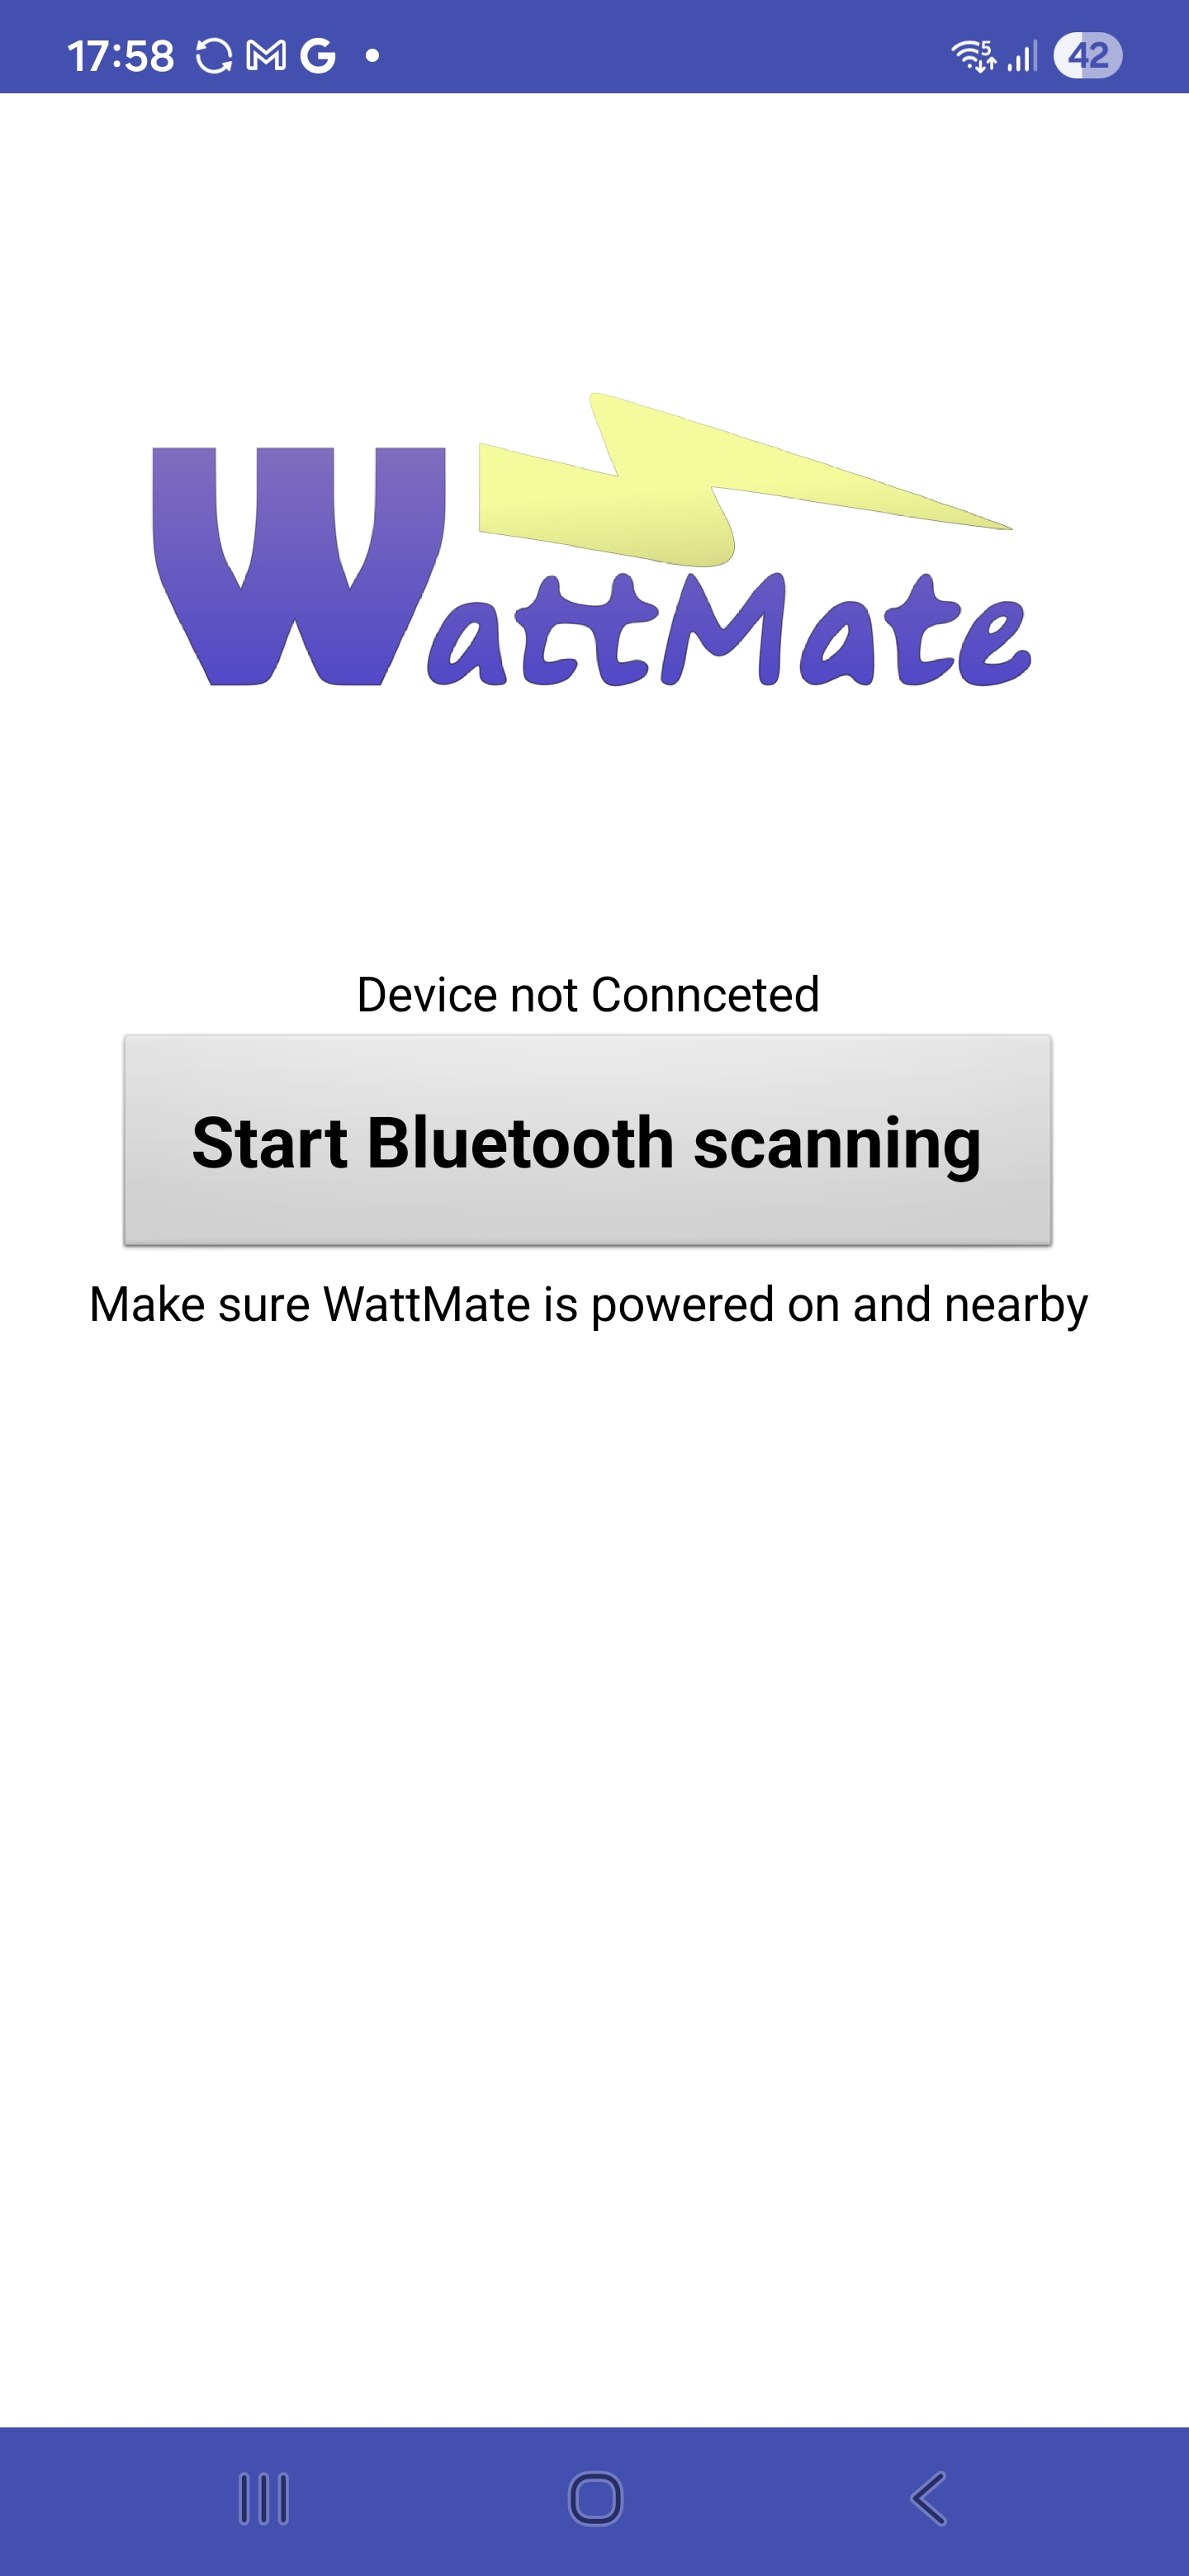
\includegraphics[width=\textwidth]{figures/3_FW_Figures/ConfigPage.jpg}
		\end{minipage}
		\hspace{1.2cm}
		\begin{minipage}{0.30\textwidth}
			\centering
			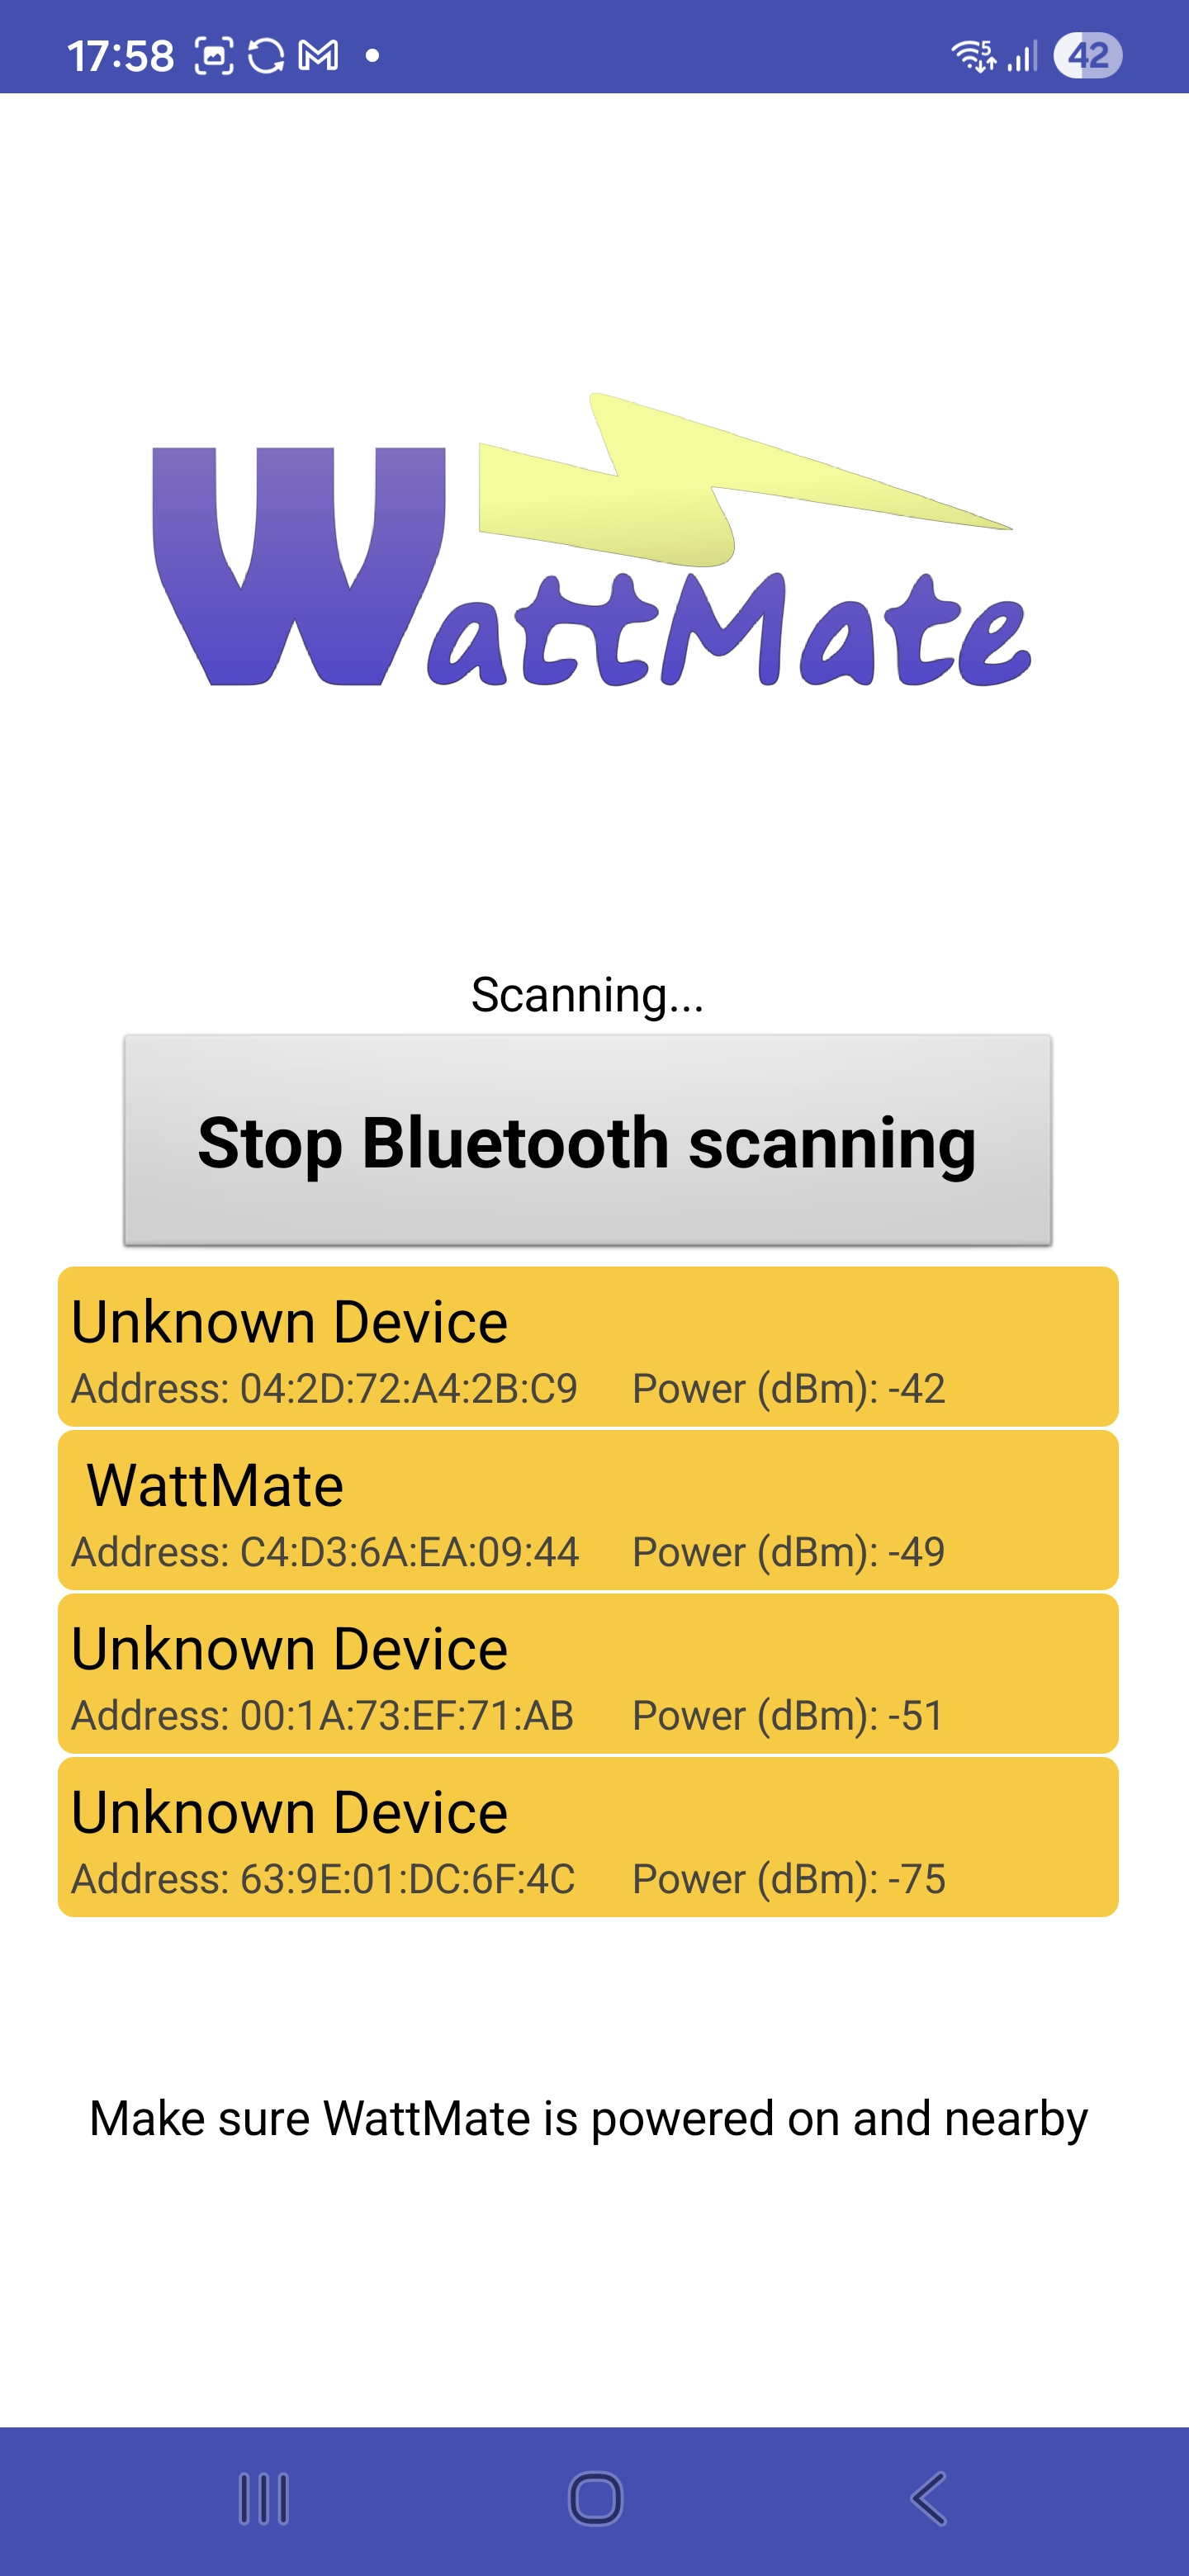
\includegraphics[width=\textwidth]{figures/3_FW_Figures/ConfigPage_BLEsearch.jpg}
		\end{minipage}
		
		\captionof{figure}{Connection page before and after pressing the "Start Bluetoth Scanning" button}
		\label{fig:App_SearchPage}
		
	\end{center}
	
	\item \textbf{Dashboard page.}
	The dashboard page is shown after a successful BLE connection. 
	It is the main view of the application and displays the connection state, the telemetry stream state, the latest update time, and the measured quantities received from WattMate. 
	It also contains the controls used to start or pause the telemetry stream, disconnect and reconnect to WattMate, or return to the device selection page. 
	Danger conditions detected by the firmware are shown through a dedicated warning banner, so that abnormal operating conditions are immediately visible during testing.
	
	\begin{center}
		\captionsetup{type=figure,width=0.70\textwidth,font=small}
		
		\begin{minipage}{0.30\textwidth}
			\centering
			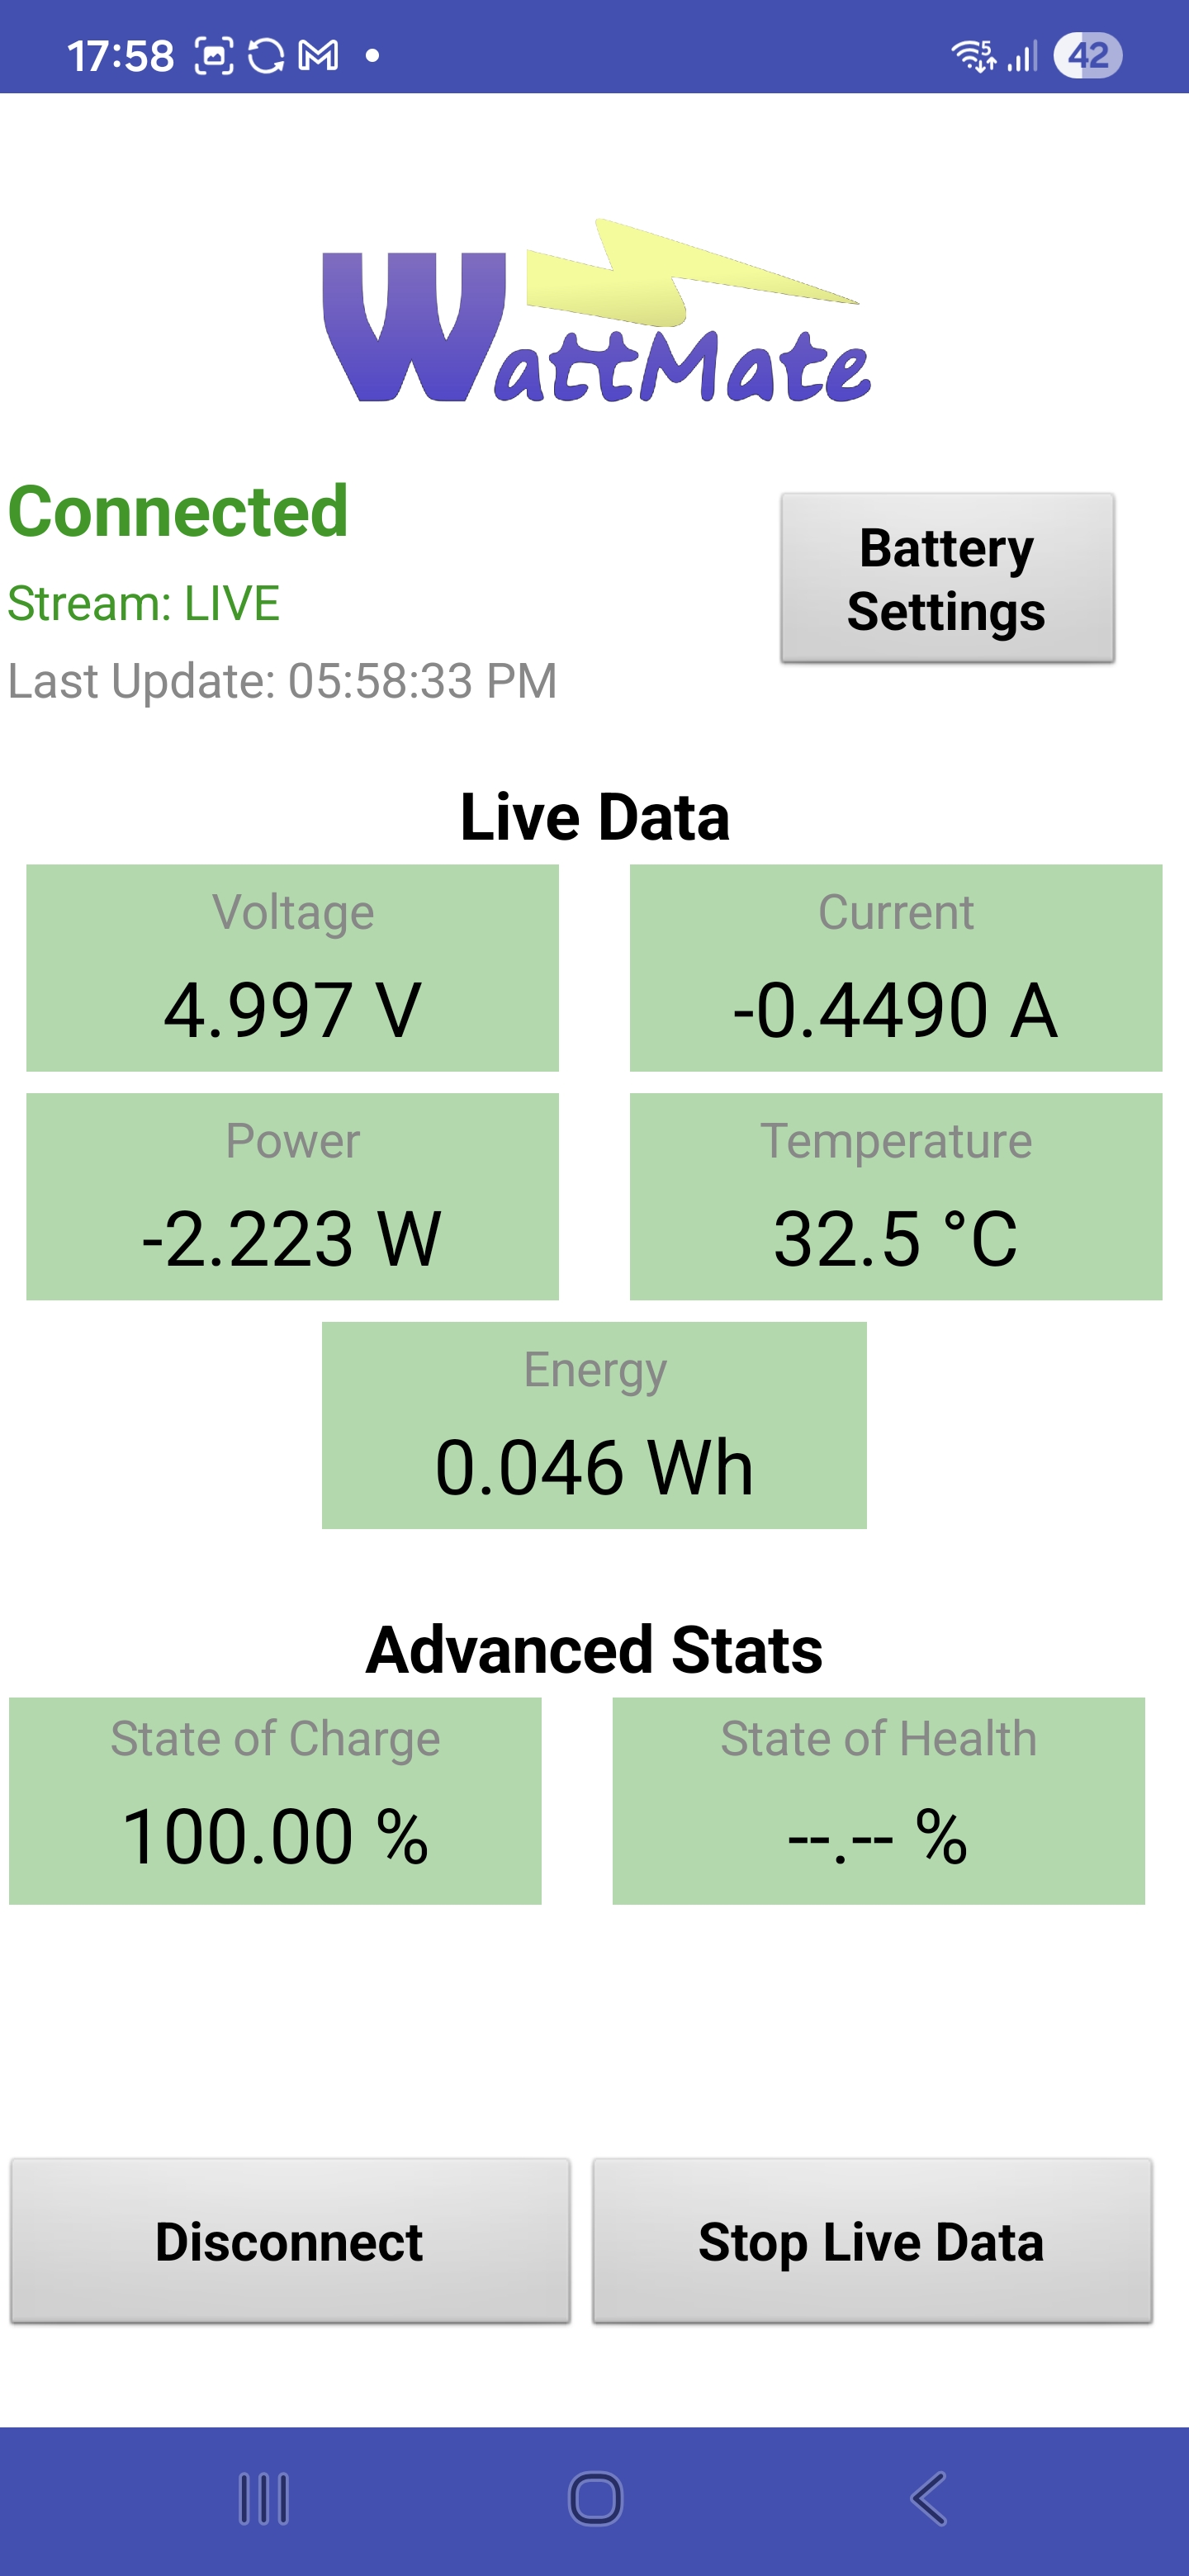
\includegraphics[width=\textwidth]{figures/3_FW_Figures/Dash.jpg}
		\end{minipage}
		\hspace{1.2cm}
		\begin{minipage}{0.30\textwidth}
			\centering
			\includegraphics[width=\textwidth]{figures/3_FW_Figures/Dash_NoStream.jpg}
		\end{minipage}
		\hspace{1.2cm}
		\begin{minipage}{0.30\textwidth}
			\centering
			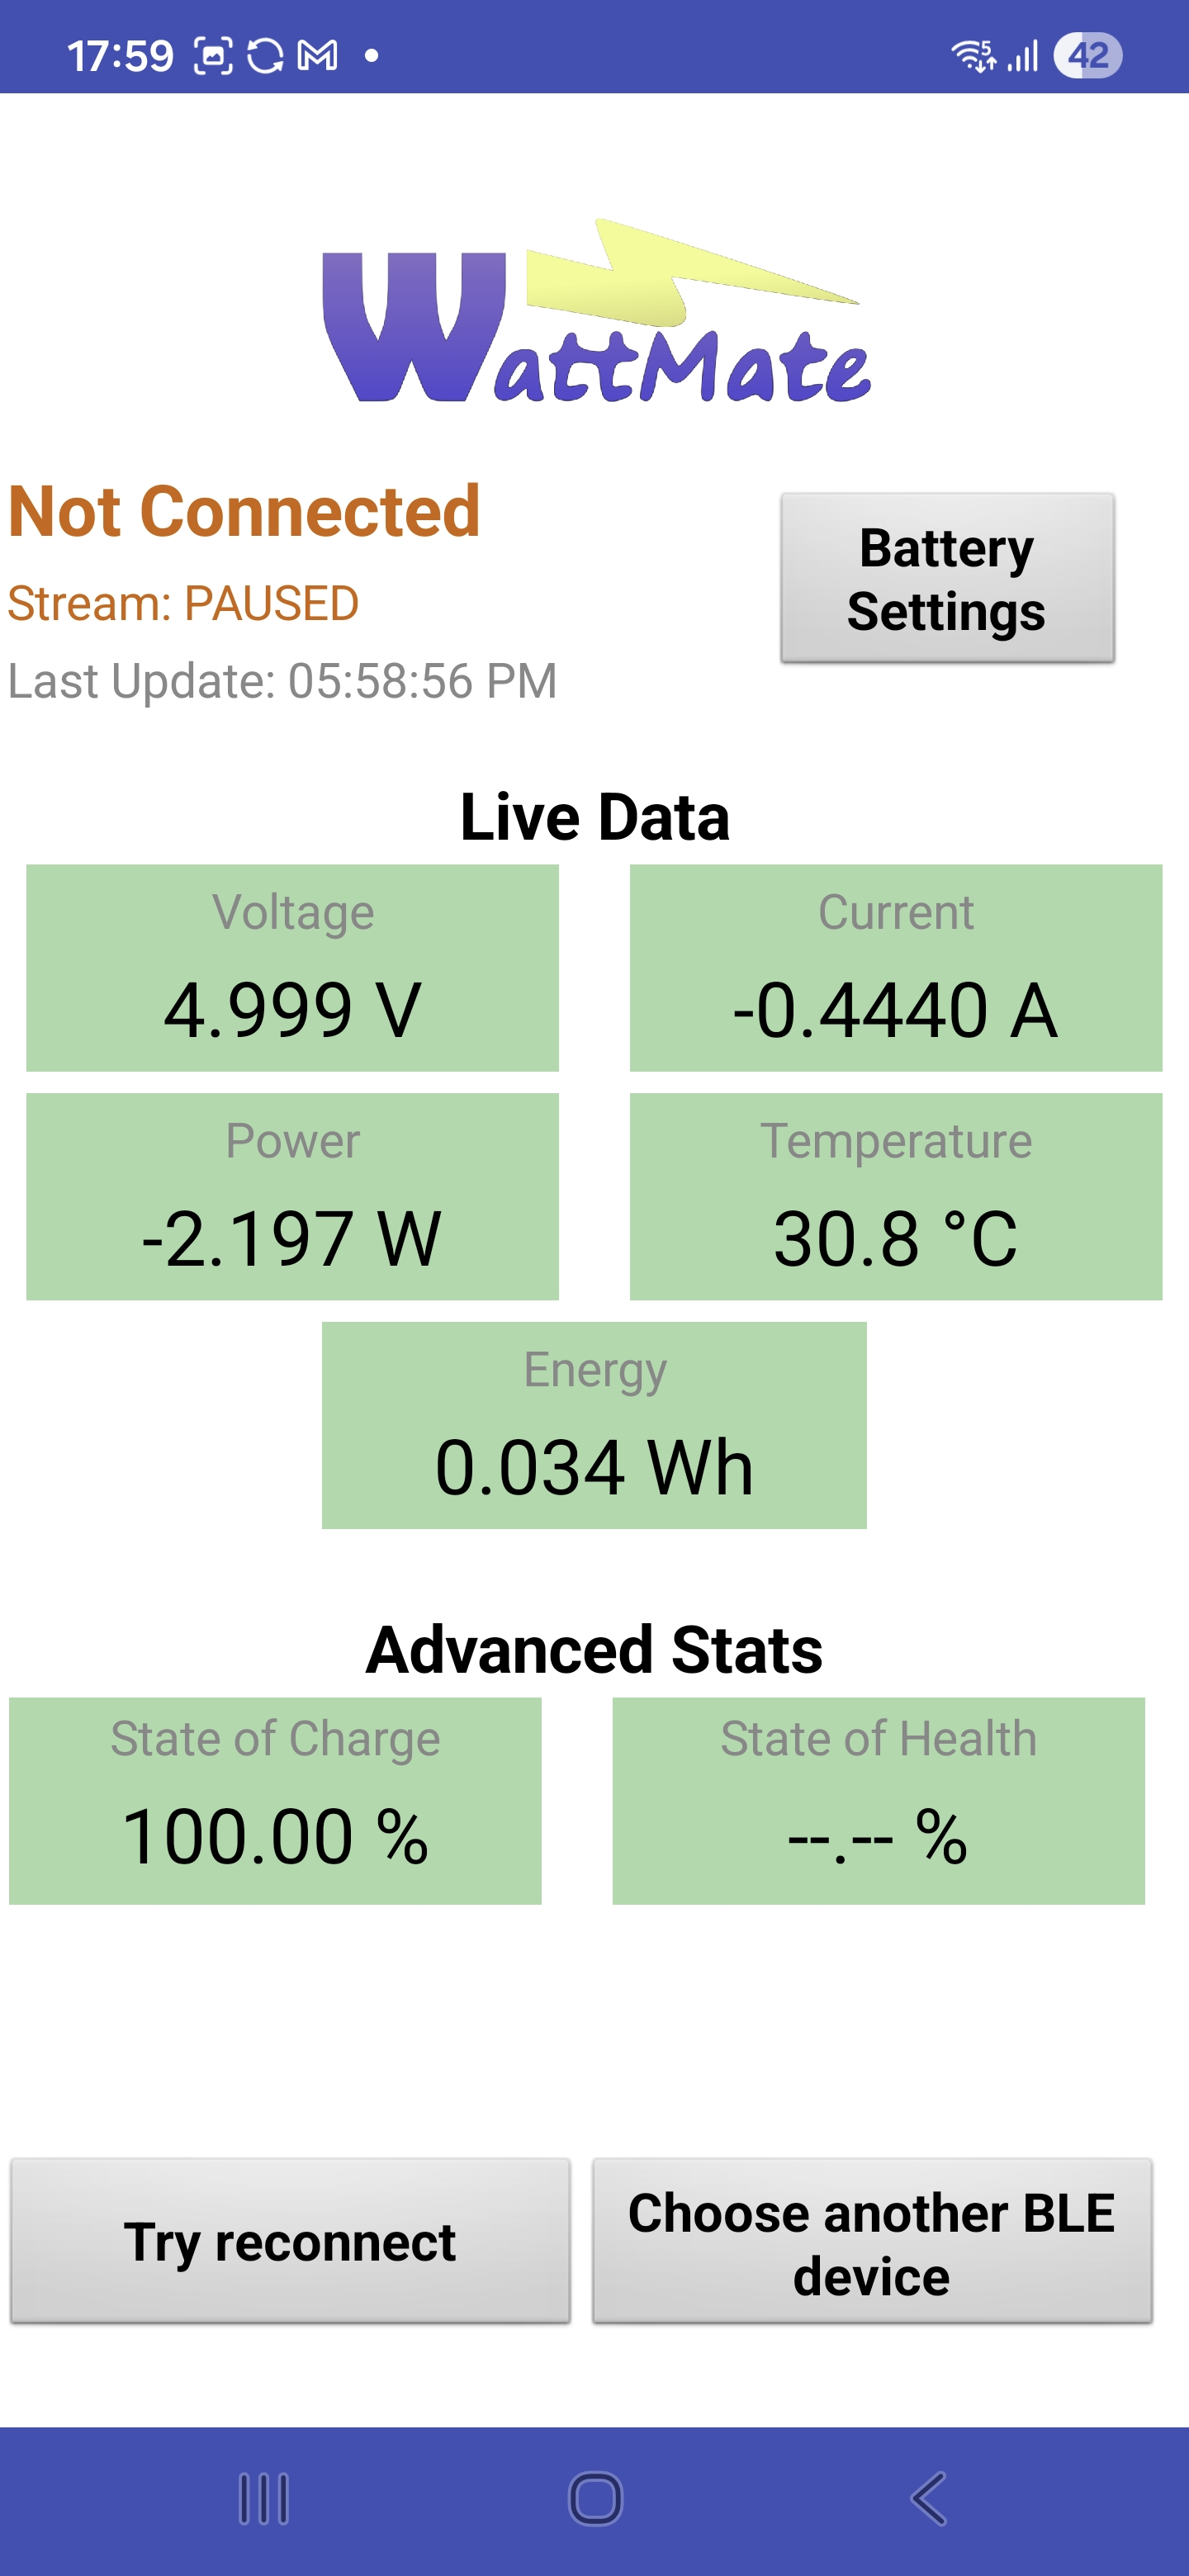
\includegraphics[width=\textwidth]{figures/3_FW_Figures/Dash_NoConn.jpg}
		\end{minipage}
		
		\captionof{figure}{Dashboard page used to display live measurements, stream state and device status}
		\label{fig:App_DashPage}
		
	\end{center}
	
	\item \textbf{Battery setup page.}
	The battery setup page is used to configure the information required by the firmware battery estimation logic. 
	The user selects the cell type from a predefined list and specifies the number of cells of that type used inside the tested power bank. 
	The application then computes the corresponding nominal battery energy and sends this value to WattMate through the dedicated BLE configuration characteristic. 
	The same page also provides a reset command to clear the stored battery estimation data, which is useful when a different battery or power bank is connected.
	
	\begin{center}
		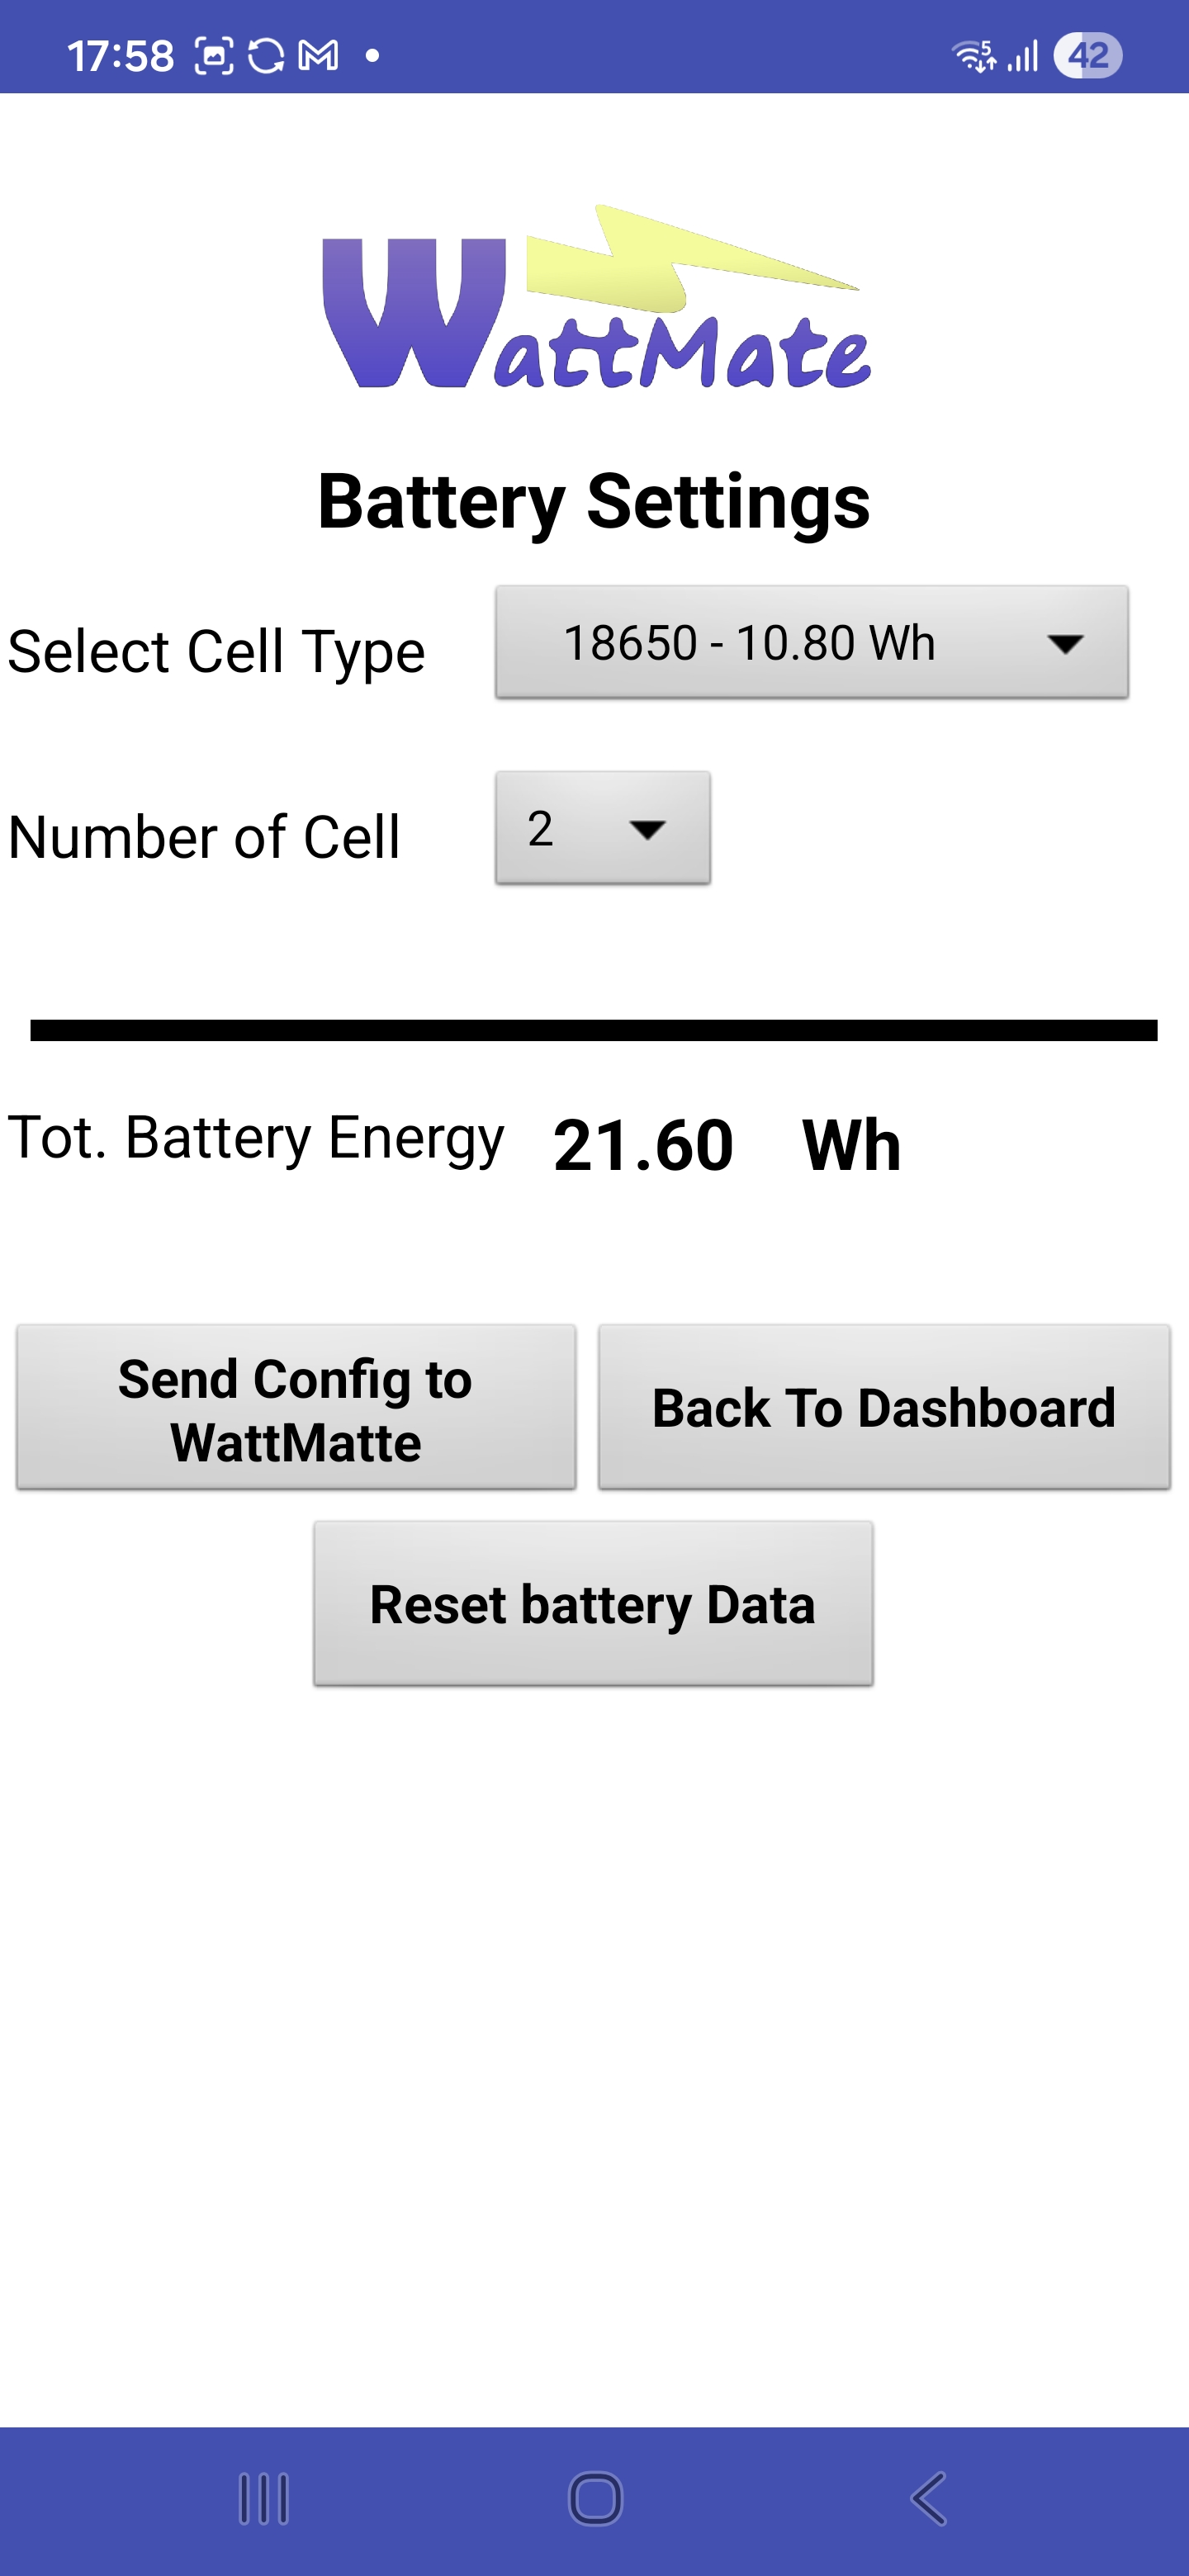
\includegraphics[width=0.30\textwidth]{figures/3_FW_Figures/BatterySettings.jpg}
		\captionof{figure}{Battery settings page, used to send the current battery setup to WattMate}
		\label{fig:App_BatterySettingsPage}
	\end{center}
\end{itemize}

This organization keeps the interface readable while preserving a simple internal structure. 
All views belong to the same App Inventor screen, and navigation is implemented only by changing the visibility of the corresponding layouts. 
This approach is sufficient for the prototype application and reduces the risk of losing the BLE state during navigation.

\section{BLE Communication Interface}
\label{sec:app_ble_interface}

The mobile application communicates with WattMate through the custom BLE service exposed by the firmware, whose structure is described in Table~\ref{tab:ble_custom_service}. 
In this chapter, the BLE interface is considered from the application side, focusing on how the Android client interacts with the characteristics published by WattMate.

After a connection is established, the application behaves differently depending on the type of characteristic exposed by the firmware:

\begin{itemize}
	\item \textbf{Notification characteristics.}
	Characteristics used for firmware-to-app data transfer are handled through BLE notifications. 
	The application must explicitly subscribe to these characteristics before receiving updates. 
	Once the subscription is active, the firmware can push new binary payloads to the phone without requiring repeated read requests from the app. 
	This mechanism is used for live telemetry, temperature updates, and battery status information.
	
	\item \textbf{Write-only characteristics.}
	Characteristics used for app-to-firmware communication are accessed through BLE write operations. 
	In this case, the application sends short binary payloads to request high-level actions or to transfer configuration values. 
	This mechanism is used to enable or disable the data stream, reset stored battery data, and send the nominal battery energy configured by the user.
\end{itemize}


\section{Connection and Stream Management}
\label{sec:app_connection_stream}

The application explicitly separates the BLE connection state from the telemetry stream state. 
A connected device is not required to continuously send telemetry notifications. 
After the BLE link has been established, the user can independently enable or disable the data stream through the control characteristic.

This separation is useful because WattMate can remain connected without continuously transmitting live measurement data. 
When the stream is disabled, the BLE link application-level traffic is reduced to the minimum required to maintain the connection. 
This significantly reduces the amount of data transmitted by the device and avoids unnecessary telemetry notifications when live values are not needed.

In the prototype application, stream control is exposed to the user through a dedicated button. 
This makes the behavior explicit during testing and allows the BLE protocol and firmware logic to be validated directly. 
In a more complete product implementation, the same mechanism could be handled automatically by the application. 
For example, the stream could be disabled when the user moves to a non-dashboard section of the app or when the app is moved to the Android background.

The current implementation does not include automatic background management, mainly because handling Android background execution would add complexity outside the main scope of the project. 
However, the implemented manual control demonstrates the required BLE and firmware functionality: the mobile application can keep the device connected while independently requesting or stopping the live telemetry stream.

\section{Displayed Data and Battery Information}
\label{sec:app_displayed_data}

The values shown by the application are directly obtained from firmware notifications. Electrical quantities are received through the telemetry characteristic, while temperature and battery status information are received through dedicated characteristics. The app only performs unit conversion and formatting.

The data received through BLE also include danger flags generated by the firmware. 
These flags are used to indicate abnormal operating conditions, such as overvoltage, overcurrent, or overtemperature. 
When at least one danger condition is active, the application displays a dedicated warning banner on the dashboard, making the condition clearly visible during testing.

It must be noted that the visualization of a danger condition on the mobile application is limited by the BLE telemetry update period. 
In the current implementation, telemetry packets are sent every \(500\,\mathrm{ms}\), so the warning banner can be updated with the same order of delay. 
This delay is acceptable for the mobile interface, because the application is only used to present the system state to the user. 
The user is not expected to take immediate safety-critical decisions based on the app visualization.

Fast reaction to abnormal operating conditions must instead be handled locally by the firmware and by the available hardware resources. 
For this reason, the danger banner should be considered a diagnostic and user-feedback feature, while the actual protection logic belongs to the embedded device.

Another interesting point is the fact that battery-related quantities are displayed together with their validity or estimation status when available. In particular, depending on the internal firmware state, the SoC, SoH and Session Energy can be unavailable, estimated, or based on a learned battery reference, as described in Section \ref{Main_Application_Task}.


\section{Battery Configuration and Control Commands}
\label{sec:app_battery_config_commands}

The mobile application is also used to send configuration and control information to the firmware. These messages are intentionally high-level: the application does not directly modify firmware internals, but requests actions that are then interpreted and applied by the embedded software.

The main configuration value sent by the app is the nominal battery energy. This value is computed from the selected cell type and the number of cells configured in the battery setup page. It is then sent to the firmware through the battery configuration characteristic. The firmware can use this value as a nominal reference for the battery total energy.

Control commands are sent through the control characteristic. They are used to enable or disable the telemetry stream and to request a full battery data reset. The reset command is intended for cases where the tested battery or power bank is replaced, so that previously learned battery information is no longer valid.

\begin{table}[H]
	\centering
	\small
	\caption{Main commands sent by the mobile application.}
	\label{tab:mobile_app_commands}
	\begin{tabularx}{\textwidth}{lX}
		\toprule
		\textbf{Command} & \textbf{Purpose} \\
		\midrule
		
		Start stream &
		Request periodic BLE telemetry notifications. \\
		
		Stop stream &
		Stop periodic BLE telemetry notifications while keeping the BLE connection active. \\
		
		Configure nominal energy &
		Send the nominal battery energy used by the firmware as battery reference. \\
		
		Reset battery data &
		Request the firmware to clear the stored battery estimation history, for example after replacing the battery or power bank. \\
		
		\bottomrule
	\end{tabularx}
\end{table}

%--------------------------------------------------

%--------------------------------------------------
% Mobile Application Design

\chapter{Interfacing and Timing}

This section describes the externally visible communication interfaces of WattMate, focusing on the associated data protocol and timing constraints.

In particular, the Bluetooth Low Energy interface is described, since it is the only digital data interface exposed to external devices. 
On the other hand, USB is not treated as a digital communication interface in this project, even though two USB-C connectors are included in the power path under measurement. 
WattMate only observes the electrical quantities associated with this power path. 
Therefore, USB data transfers and the related communication protocols are ignored by the device.

Internal interfaces used for measurement acquisition, display update, and firmware task communication are described in the hardware and firmware sections. 
They are not described in detail in this section, since they are not relevant to an external device connecting to WattMate according to the intended use model.


\section{Bluetooth Low Energy Protocol Overview}
\label{sec:ble_protocol_overview}

This section introduces the Bluetooth Low Energy mechanisms required to understand the WattMate external interface. 
Only the parts of the protocol that are relevant for this project are described: device discovery through advertising, connection management through GAP, and application data exchange through ATT/GATT. 
The WattMate-specific advertising data, GATT characteristics, payload formats, and timing diagrams are reported in Section~\ref{sec:wattmate_ble_interface_behaviour}.

\subsection{Advertising and Device Discovery}
\label{sec:ble_advertising_discovery}

Bluetooth Low Energy advertising is the standard mechanism used by a peripheral device to periodically announce its presence before a connection is established. 
Nearby central devices can scan for these packets, inspect the advertised information, and decide whether to initiate a connection.

In the Bluetooth specification, packet field sizes are expressed in \emph{octets}. 
An octet corresponds to an 8-bit byte; the standard term is kept in this section to remain consistent with the BLE nomenclature.

At Link Layer level, a BLE packet is composed of four main fields: preamble, access address, Protocol Data Unit (PDU), and cyclic redundancy check. 
The first and last fields support synchronization and error detection, while the PDU is the field that carries the protocol information exchanged between devices~\cite{bluetooth_core_link_layer}. 
The simplified packet structure is shown in Figure~\ref{fig:ble_ll_packet_format}.

\begin{figure}[H]
	\centering
	\small
	\renewcommand{\arraystretch}{1.25}
	\begin{tabular}{|c|c|c|c|}
		\hline
		\textbf{Preamble} & \textbf{Access Address} & \textbf{PDU} & \textbf{CRC} \\
		\hline
		1 octet & 4 octets & variable & 3 octets \\
		\hline
	\end{tabular}
	\caption{BLE Link Layer packet format.}
	\label{fig:ble_ll_packet_format}
\end{figure}

For advertising packets, the PDU can be represented as a header followed by a variable-length payload. 
The header specifies the advertising PDU type and the payload length, while the payload carries the information associated with the advertising event~\cite{bluetooth_core_link_layer}.

\begin{figure}[H]
	\centering
	\small
	\renewcommand{\arraystretch}{1.25}
	\begin{tabular}{|c|c|}
		\hline
		\textbf{Advertising PDU Header} & \textbf{Advertising PDU Payload} \\
		\hline
		2 octets & variable length \\
		\hline
	\end{tabular}
	\caption{BLE advertising PDU format.}
	\label{fig:ble_adv_pdu_format}
\end{figure}

The discovery information inside the advertising payload is encoded as a sequence of Advertising Data structures. 
Each structure contains a length field, an Advertising Data type, and the associated data. 
The type field defines how the following octets must be interpreted by the scanner~\cite{bluetooth_css_data_types}.

\begin{figure}[H]
	\centering
	\small
	\renewcommand{\arraystretch}{1.25}
	\begin{tabular}{|c|c|c|}
		\hline
		\textbf{Length} & \textbf{AD Type} & \textbf{AD Data} \\
		\hline
		1 octet & 1 octet & Length - 1 octets \\
		\hline
	\end{tabular}
	\caption{Generic Advertising Data structure.}
	\label{fig:ble_ad_structure}
\end{figure}


Advertising timing is mainly controlled by the advertising interval. 
A shorter interval reduces the expected discovery time, while a longer interval reduces the amount of wireless activity. 
The Bluetooth specification also adds a small pseudo-random advertising delay to the configured interval, in order to reduce the probability of repeated collisions between advertisers~\cite{bluetooth_core_link_layer}.

The project-specific advertising configuration, including the advertised fields, scan response content, and selected timing values, is reported in Section~\ref{sec:wattmate_advertising_data}.





\subsection{GAP Roles and Connection Management}
\label{sec:ble_connection_roles}

The Generic Access Profile (GAP) defines the procedures and roles used by BLE devices to become discoverable, establish a link, terminate a link, and manage the basic parameters of a connection~\cite{bluetooth_core_gap}. 
For the connected use case considered in this project, the relevant GAP roles are the central and the peripheral.

\paragraph{Central and peripheral roles.}
After a peripheral device has been discovered through advertising, a central device can initiate a BLE connection. 
The peripheral is the device that advertises and accepts the connection, while the central is the device that scans, selects the peripheral, and starts the connection procedure.

\begin{table}[H]
	\centering
	\small
	\caption{BLE central and peripheral roles during discovery and connection establishment.}
	\label{tab:ble_connection_roles}
	\begin{tabular}{p{0.22\textwidth} p{0.30\textwidth} p{0.30\textwidth}}
		\toprule
		\textbf{Phase} & \textbf{Central role} & \textbf{Peripheral role} \\
		\midrule
		Discovery &
		Scans for advertising packets. &
		Advertises its presence. \\
		
		Connection setup &
		Initiates the connection. &
		Accepts the connection. \\
		\bottomrule
	\end{tabular}
\end{table}

The central and peripheral roles define how the BLE link is established and maintained, but they do not impose a fixed direction for application data once the connection is active. 
Data exchange is handled by the upper protocol layers, mainly through ATT/GATT in the use case considered in this report.

After the BLE link has been established, the central device can discover the GATT database exposed by the peripheral. 
This discovery phase allows the central to identify the available services, characteristics, and supported access operations before starting the actual application data exchange~\cite{bluetooth_core_gatt}. 
The GATT data model is described in Section~\ref{sec:ble_gatt_data_model}.




\paragraph{Connection events.}
A BLE connection is organized into periodic connection events. 
A connection event is a time window in which the two devices can exchange Link Layer packets. 
These packets may carry Link Layer control information or data produced by upper protocol layers. 
For application-level BLE communication, the relevant upper-layer traffic is typically carried through ATT/GATT, described in Section~\ref{sec:ble_gatt_data_model}. 
Therefore, a connection event does not imply that a new application value is exchanged; it only defines when packet exchange can occur and helps keep the two devices synchronized.




\paragraph{Connection timing parameters.}
The timing behaviour of a BLE connection is controlled by a set of standard parameters. 
The parameters most relevant to an application using periodic data exchange are summarized in Table~\ref{tab:ble_connection_parameters}. 
They define the timing of the BLE link, while the application protocol independently defines when new data are produced and sent.

\begin{table}[H]
	\centering
	\small
	\caption{Main BLE connection parameters relevant to application-level timing.}
	\label{tab:ble_connection_parameters}
	\begin{tabularx}{\textwidth}{l X}
		\toprule
		\textbf{Parameter} &  \textbf{Meaning} \\
		\midrule
		Connection interval &
		Time between the start of two consecutive connection events. It defines how often the devices have the opportunity to exchange packets during an active connection. \\
		
		Peripheral latency &
		Maximum number of consecutive connection events that the peripheral may skip when it has no data to exchange. This can reduce wireless activity while keeping the connection active. \\
		
		Supervision timeout &
		Maximum allowed time without a successful connection event before the connection is considered lost. \\
		
		PHY mode &
		Physical layer mode used by the link, such as LE 1M PHY or LE 2M PHY. It affects packet airtime and achievable throughput, but it does not directly define the application update period. \\
		\bottomrule
	\end{tabularx}
\end{table}

During an active connection, some parameters can be updated using standard BLE procedures. 
For example, the connection interval can be changed to modify the latency and activity of the link, and the PHY mode can be updated if both devices support the requested mode~\cite{bluetooth_core_link_layer}. 
The project-specific connection sequence and selected timing values are reported in Section~\ref{sec:wattmate_connection_timing}.



\subsection{ATT and GATT Data Model}
\label{sec:ble_gatt_data_model}

At application level, BLE data are commonly organized using the Generic Attribute Profile (GATT), which is built on top of the Attribute Protocol (ATT). 
ATT provides the attribute-based access mechanism, while GATT defines how these attributes are structured into services, characteristics, values, and descriptors~\cite{bluetooth_core_gatt}.

A GATT server exposes a database of attributes. 
A GATT client accesses this database to discover the available services and to interact with the characteristic values exposed by the server. 
A service groups related data objects, while each characteristic represents one specific data item or control point. 
Each characteristic has one value and may include one or more descriptors, used to provide additional information or configuration associated with that characteristic.

\begin{figure}[H]
	\centering
	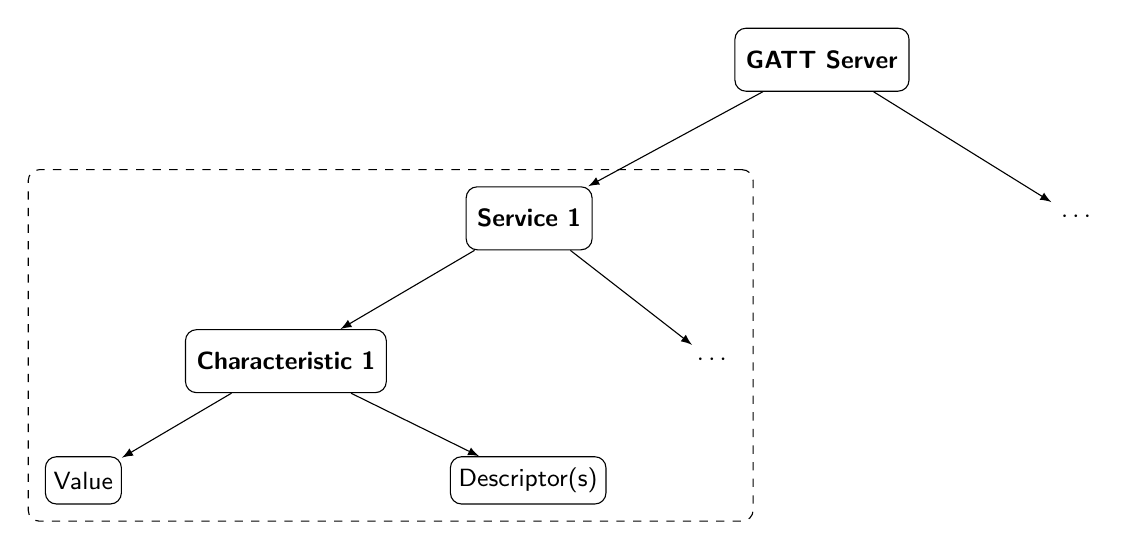
\begin{tikzpicture}[
		font=\small,
		node distance=6mm and 10mm,
		box/.style={draw, rounded corners, align=center, minimum height=8mm, inner sep=4pt},
		smallbox/.style={draw, rounded corners, align=center, minimum height=6mm, inner sep=3pt},
		group/.style={draw, rounded corners, dashed, inner sep=6pt}
		]
		
		% Top level
		\node[box] (server) {\textbf{GATT Server}};
		
		% Services
		\node[box, below left=12mm and 18mm of server] (service1) {\textbf{Service 1}};
		\node[below right=14mm and 18mm of server] (more_services) {\(\cdots\)};
		
		\draw[-latex] (server) -- (service1);
		\draw[-latex] (server) -- (more_services);
		
		% Characteristics under Service 1
		\node[box, below left=10mm and 10mm of service1] (char11) {\textbf{Characteristic 1}};
		\node[below right=12mm and 12mm of service1] (more_chars) {\(\cdots\)};
		
		\draw[-latex] (service1) -- (char11);
		\draw[-latex] (service1) -- (more_chars);
		
		% Characteristic internal structure
		\node[smallbox, below left=8mm and 8mm of char11] (val11) {Value};
		\node[smallbox, below right=8mm and 8mm of char11] (desc11) {Descriptor(s)};
		
		\draw[-latex] (char11) -- (val11);
		\draw[-latex] (char11) -- (desc11);
		
		% Dashed contour around the whole service subtree
		\node[group, fit=(service1)(char11)(more_chars)(val11)(desc11)] {};
		
	\end{tikzpicture}
	\caption{Simplified hierarchical organization of a GATT server.}
	\label{fig:ble_gatt_data_model}
\end{figure}


\paragraph{Data exchange procedures.}
Once the GATT database has been discovered, the client can interact with the exposed characteristics according to their access properties.

At ATT level, each operation is encoded as an ATT Protocol Data Unit. 
The procedures considered in this report can be represented, in simplified form, by an opcode, an attribute handle, and an optional value field~\cite{bluetooth_core_att}. 
The opcode identifies the operation, the handle identifies the target attribute inside the GATT database, and the value field carries the data associated with the operation.

\begin{figure}[H]
	\centering
	\small
	\renewcommand{\arraystretch}{1.25}
	\begin{tabular}{|c|c|c|}
		\hline
		\textbf{Opcode} & \textbf{Attribute Handle} & \textbf{Value} \\
		\hline
		1 octet & 2 octets & variable length \\
		\hline
	\end{tabular}
	\caption{Simplified ATT PDU structure for characteristic value operations.}
	\label{fig:ble_att_pdu_format}
\end{figure}

For a characteristic write, the handle identifies the writable characteristic value and the value field contains the data written by the client. 
For a characteristic notification, the handle identifies the notified characteristic value and the value field contains the data sent by the server. 
CCCD configuration follows the same principle, but the handle refers to the Client Characteristic Configuration Descriptor associated with the characteristic.

The procedures relevant for this project are summarized in Table~\ref{tab:ble_gatt_procedures}.

\begin{table}[H]
	\centering
	\small
	\caption{GATT procedures relevant to application data exchange.}
	\label{tab:ble_gatt_procedures}
	\begin{tabular}{p{0.22\textwidth} p{0.25\textwidth} p{0.43\textwidth}}
		\toprule
		\textbf{Mechanism} & \textbf{Direction} & \textbf{Purpose} \\
		\midrule
		Characteristic write &
		Client to server \newline
		\emph{App to WattMate} &
		The client writes a new value into a writable characteristic exposed by the server. 
		This mechanism is suitable for commands or configuration values. \\
		
		Characteristic notification &
		Server to client \newline
		\emph{WattMate to App} &
		The server sends an updated characteristic value to the client without requiring continuous polling. 
		Notifications do not generate a specific GATT-level response from the client. \\
		
		CCCD configuration &
		Client to server \newline
		\emph{App to WattMate} &
		The client writes the Client Characteristic Configuration Descriptor to enable or disable notifications or indications for a characteristic that supports them. \\
		\bottomrule
	\end{tabular}
\end{table}


This model separates the logical application protocol from the low-level BLE packet exchange. 
The application only needs to define which services and characteristics are exposed, which access mechanisms are allowed, and how each characteristic value must be interpreted.

The project-specific GATT service, characteristic UUIDs, access properties, CCCD usage, and payload formats are reported in Section~\ref{sec:wattmate_custom_gatt_service}.








\section{WattMate BLE Interface Behaviour}
\label{sec:wattmate_ble_interface_behaviour}

This section describes the externally visible behaviour of the WattMate BLE interface. 
The diagrams are given at protocol level: they do not represent the bit-level timing of BLE packets, but the sequence and periodicity of the operations that are relevant for discovery, connection setup, and measurement streaming.

\subsection{Advertising Configuration and Timing}
\label{sec:wattmate_advertising_data}

WattMate uses legacy connectable and scannable BLE advertising for discovery and connection establishment. 
The main advertising packet contains the standard flags and the complete local name \texttt{WattMate}, while the scan response contains the 128-bit UUID of the custom WattMate data service. 
No measurement data are transmitted during advertising.

Two advertising profiles are used. 
Fast advertising is used after startup or explicit user interaction to reduce discovery latency. 
If no connection is established within \(20\,\mathrm{s}\), WattMate switches to slow advertising to reduce wireless activity while remaining discoverable.

\begin{table}[H]
	\centering
	\small
	\caption{WattMate advertising profiles.}
	\label{tab:wattmate_advertising_profiles}
	\begin{tabular}{p{0.25\textwidth} p{0.22\textwidth} p{0.38\textwidth}}
		\toprule
		\textbf{Profile} & \textbf{Interval} & \textbf{Use} \\
		\midrule
		Fast advertising &
		\(100\,\mathrm{ms}\) &
		Used after startup or explicit user interaction to make the device easier to discover. \\
		
		Slow advertising &
		\(1000\,\mathrm{ms}\) &
		Used after the fast advertising window when no connection has been established. \\
		\bottomrule
	\end{tabular}
\end{table}

\begin{figure}[H]
	\centering
	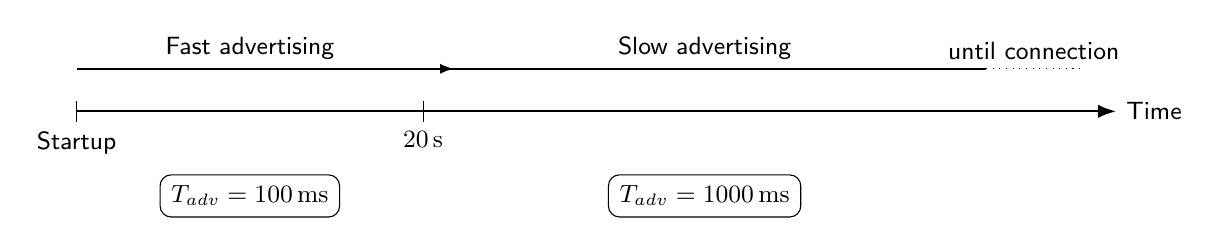
\begin{tikzpicture}[
		x=0.55cm,
		y=0.9cm,
		font=\small,
		axis/.style={-Latex, thick},
		box/.style={draw, rounded corners, align=center, inner sep=4pt}
		]
		% Time axis
		\draw[axis] (0,0) -- (24,0) node[right] {Time};
		
		% Phase bars
		\draw[thick] (0,0.6) -- (8,0.6);
		\draw[thick] (8,0.6) -- (21,0.6);
		
		% Ticks
		\draw (0,0.15) -- (0,-0.15) node[below] {Startup};
		\draw (8,0.15) -- (8,-0.15) node[below] {\(20\,\mathrm{s}\)};
		\draw[dotted] (21,0.6) -- (23.2,0.6);
		\node[above] at (22.1,0.6) {until connection};
		
		% Labels
		\node[above] at (4,0.6) {Fast advertising};
		\node[above] at (14.5,0.6) {Slow advertising};
		
		\node[box, below=8mm] at (4,0) {\(T_{adv}=100\,\mathrm{ms}\)};
		\node[box, below=8mm] at (14.5,0) {\(T_{adv}=1000\,\mathrm{ms}\)};
		
		\draw[-Latex] (7.3,0.6) -- (8.7,0.6);
	\end{tikzpicture}
	\caption{WattMate advertising timing before connection establishment.}
	\label{fig:wattmate_advertising_timing}
\end{figure}

\subsection{Custom GATT Service and Characteristics}
\label{sec:wattmate_custom_gatt_service}

After a BLE connection has been established, WattMate exposes its data through a custom GATT service. 
All UUIDs used by the service follow the same base format:
\[
\texttt{f000xxxx-0451-4000-b000-000000000000}
\]
where \texttt{xxxx} identifies the specific service or characteristic.

All multi-byte numeric fields transmitted by the WattMate GATT interface use little-endian byte order. 
Payloads are binary and fixed-size, so an external BLE client can decode each characteristic value directly from its byte layout.

\begin{table}[H]
	\centering
	\small
	\caption{WattMate custom GATT service and characteristics.}
	\label{tab:wattmate_gatt_characteristics}
	\begin{tabular}{p{0.24\textwidth} p{0.16\textwidth} p{0.16\textwidth} p{0.12\textwidth} p{0.22\textwidth}}
		\toprule
		\textbf{Name} & \textbf{UUID field} & \textbf{Property} & \textbf{Size} & \textbf{Direction} \\
		\midrule
		Data Service &
		\texttt{0x1130} &
		Service &
		-- &
		-- \\
		
		Telemetry &
		\texttt{0x1131} &
		Notify &
		17 B &
		WattMate to App \\
		
		Temperature &
		\texttt{0x1132} &
		Notify &
		2 B &
		WattMate to App \\
		
		Control &
		\texttt{0x1133} &
		Write &
		1 B &
		App to WattMate \\
		
		Battery Config &
		\texttt{0x1134} &
		Write &
		2 B &
		App to WattMate \\
		
		Battery Status &
		\texttt{0x1135} &
		Notify &
		2 B &
		WattMate to App \\
		\bottomrule
	\end{tabular}
\end{table}

\paragraph{Telemetry characteristic.}
The Telemetry characteristic contains the main live electrical measurements and status flags.

\begin{table}[H]
	\centering
	\small
	\caption{Telemetry characteristic payload format.}
	\label{tab:wattmate_telemetry_payload}
	\begin{tabular}{p{0.13\textwidth} p{0.12\textwidth} p{0.16\textwidth} p{0.20\textwidth} p{0.29\textwidth}}
		\toprule
		\textbf{Offset} & \textbf{Size} & \textbf{Type} & \textbf{Field} & \textbf{Encoding} \\
		\midrule
		0--1 &
		2 B &
		\texttt{uint16} &
		Voltage &
		Bus voltage in millivolts. \\
		
		2--5 &
		4 B &
		\texttt{int32} &
		Current &
		Load current in microamperes. \\
		
		6--9 &
		4 B &
		\texttt{int32} &
		Power &
		Instantaneous power in microwatts. \\
		
		10--13 &
		4 B &
		\texttt{uint32} &
		Session energy &
		Accumulated session energy in microwatt-hours. \\
		
		14 &
		1 B &
		\texttt{uint8} &
		Danger flags &
		Bitfield described in Table~\ref{tab:wattmate_danger_flags}. \\
		
		15--16 &
		2 B &
		\texttt{uint16} &
		State of Charge &
		Percentage multiplied by 100. \texttt{10000} represents \(100.00\%\); \texttt{0xFFFF} represents an unknown value. \\
		\bottomrule
	\end{tabular}
\end{table}

Bit numbering starts from bit~0 as the least significant bit of the byte.

\begin{table}[H]
	\centering
	\small
	\caption{Telemetry danger flags bitfield.}
	\label{tab:wattmate_danger_flags}
	\begin{tabular}{p{0.16\textwidth} p{0.28\textwidth} p{0.46\textwidth}}
		\toprule
		\textbf{Bit} & \textbf{Flag} & \textbf{Meaning} \\
		\midrule
		0 &
		Overvoltage &
		Set when the measured voltage is above the configured safe range. \\
		
		1 &
		Overcurrent &
		Set when the measured current is above the configured safe range. \\
		
		2 &
		Overtemperature &
		Protocol-defined temperature warning flag. \\
		
		7--3 &
		Reserved &
		Reserved for future use and currently cleared. \\
		\bottomrule
	\end{tabular}
\end{table}

\paragraph{Temperature characteristic.}
The Temperature characteristic contains the temperature measured by the NTC sensor.

\begin{table}[H]
	\centering
	\small
	\caption{Temperature characteristic payload format.}
	\label{tab:wattmate_temperature_payload}
	\begin{tabular}{p{0.13\textwidth} p{0.12\textwidth} p{0.16\textwidth} p{0.20\textwidth} p{0.29\textwidth}}
		\toprule
		\textbf{Offset} & \textbf{Size} & \textbf{Type} & \textbf{Field} & \textbf{Encoding} \\
		\midrule
		0--1 &
		2 B &
		\texttt{int16} &
		Temperature &
		Temperature in centi-degrees Celsius. For example, \texttt{2534} represents \(25.34\,^{\circ}\mathrm{C}\). \\
		\bottomrule
	\end{tabular}
\end{table}

\paragraph{Control characteristic.}
The Control characteristic is a 1-byte bitfield written by the mobile application. 
Reserved bits must be kept cleared.

\begin{table}[H]
	\centering
	\small
	\caption{Control characteristic payload format.}
	\label{tab:wattmate_control_payload}
	\begin{tabular}{p{0.16\textwidth} p{0.28\textwidth} p{0.46\textwidth}}
		\toprule
		\textbf{Bit} & \textbf{Field} & \textbf{Meaning} \\
		\midrule
		0 &
		Stream enable &
		When set to 1, the measurement stream is enabled. When cleared, the stream is disabled. \\
		
		1 &
		Battery data reset &
		When set to 1, a reset of the battery-related data is requested. \\
		
		7--2 &
		Reserved &
		Reserved bits. They must be written as 0. \\
		\bottomrule
	\end{tabular}
\end{table}

\paragraph{Battery Config characteristic.}
The Battery Config characteristic is used to provide the nominal energy of the battery under test.

\begin{table}[H]
	\centering
	\small
	\caption{Battery Config characteristic payload format.}
	\label{tab:wattmate_battery_config_payload}
	\begin{tabular}{p{0.13\textwidth} p{0.12\textwidth} p{0.16\textwidth} p{0.20\textwidth} p{0.29\textwidth}}
		\toprule
		\textbf{Offset} & \textbf{Size} & \textbf{Type} & \textbf{Field} & \textbf{Encoding} \\
		\midrule
		0--1 &
		2 B &
		\texttt{uint16} &
		Nominal energy &
		Nominal battery energy in centi-watt-hours. \\
		\bottomrule
	\end{tabular}
\end{table}

\paragraph{Battery Status characteristic.}
The Battery Status characteristic contains the estimated battery State of Health.

\begin{table}[H]
	\centering
	\small
	\caption{Battery Status characteristic payload format.}
	\label{tab:wattmate_battery_status_payload}
	\begin{tabular}{p{0.13\textwidth} p{0.12\textwidth} p{0.16\textwidth} p{0.20\textwidth} p{0.29\textwidth}}
		\toprule
		\textbf{Offset} & \textbf{Size} & \textbf{Type} & \textbf{Field} & \textbf{Encoding} \\
		\midrule
		0--1 &
		2 B &
		\texttt{uint16} &
		State of Health &
		Percentage multiplied by 100. \texttt{10000} represents \(100.00\%\); \texttt{0xFFFF} represents an unknown value. \\
		\bottomrule
	\end{tabular}
\end{table}



\subsection{WattMate BLE Timing Parameters}
\label{sec:wattmate_ble_timing_parameters}

The main BLE timing parameters used by WattMate are summarized in Table~\ref{tab:wattmate_ble_timing_parameters}. 
These values describe the externally relevant timing behaviour of the interface. 
BLE connection events may occur more frequently than the application data updates; therefore, the notification periods reported in the table must be interpreted as application-level streaming periods, not as BLE connection intervals.

\begin{table}[H]
	\centering
	\small
	\caption{WattMate BLE timing parameters.}
	\label{tab:wattmate_ble_timing_parameters}
	\begin{tabular}{p{0.28\textwidth} p{0.22\textwidth} p{0.40\textwidth}}
		\toprule
		\textbf{Parameter} & \textbf{Value} & \textbf{Meaning} \\
		\midrule
		Fast advertising interval &
		\(100\,\mathrm{ms}\) &
		Advertising interval used after startup or explicit user interaction to reduce discovery latency. \\
		
		Fast advertising window &
		\(20\,\mathrm{s}\) &
		Maximum duration of the fast advertising phase before switching to slow advertising if no connection is established. \\
		
		Slow advertising interval &
		\(1000\,\mathrm{ms}\) &
		Advertising interval used to keep the device discoverable with lower BLE activity. \\
		
		Preferred connection interval &
		\(15\,\mathrm{ms}\) to \(45\,\mathrm{ms}\) &
		Preferred BLE connection interval range requested by WattMate after connection establishment. The final value depends on the central device. \\
		
		Preferred peripheral latency &
		\(0\) &
		Requested value for peripheral latency, meaning that WattMate does not request to skip connection events. \\
		
		Supervision timeout &
		\(2\,\mathrm{s}\) &
		Maximum time without a successful connection event before the BLE link is considered lost. \\
		
		Connection parameter update delay &
		\(6000\,\mathrm{ms}\) &
		Delay after connection establishment before requesting the preferred connection timing parameters. \\
		
		Preferred PHY &
		LE 2M PHY &
		Preferred physical layer mode requested after connection establishment, if supported by the central device. \\
		
		Telemetry notification period &
		\(500\,\mathrm{ms}\) &
		Application-level period for live telemetry notifications. \\
		
		Temperature notification period &
		\(500\,\mathrm{ms}\) &
		Application-level period for temperature notifications. \\
		
		Battery status notification period &
		Immediate at stream start, then about \(10.5\,\mathrm{s}\) &
		Battery status is sent once when the stream starts and then at a slower rate than live measurements. \\
		
		RSSI update period &
		\(1000\,\mathrm{ms}\) &
		Period used to update the connection RSSI value while the device is connected. \\
		\bottomrule
	\end{tabular}
\end{table}



\subsection{Connection and Stream Setup}
\label{sec:wattmate_connection_timing}

After discovery, the mobile application connects to WattMate and discovers the exposed GATT service. 
Before streamed data can be received, the application enables notifications on the notified characteristics by configuring the corresponding CCCDs. 
The measurement stream is then started through a write to the Control characteristic.

\begin{figure}[H]
	\centering
	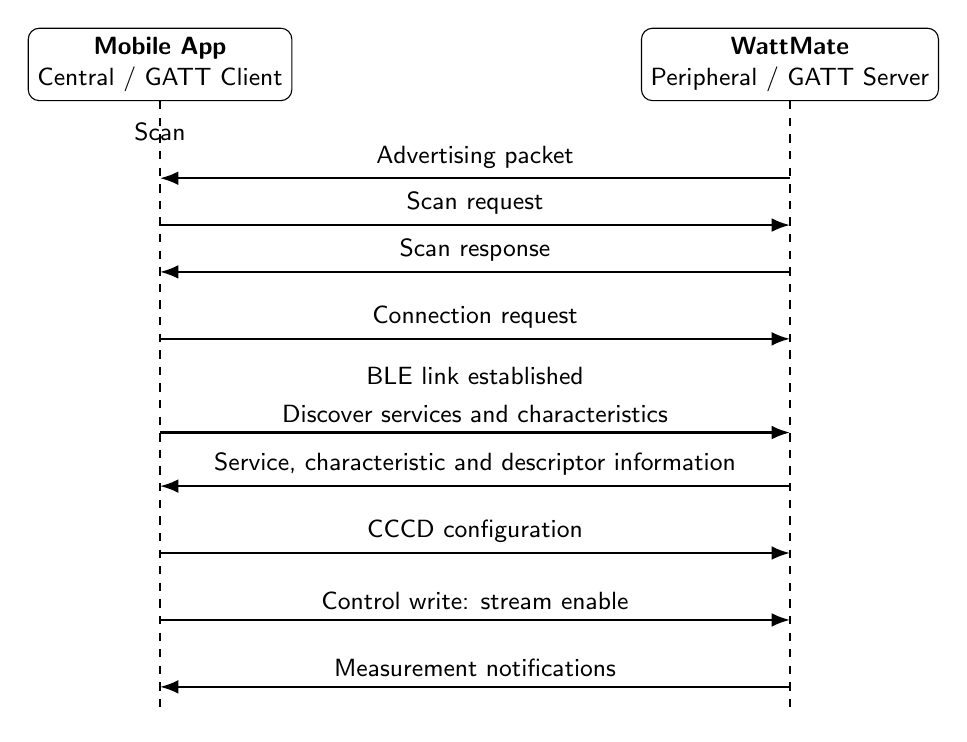
\begin{tikzpicture}[
		x=1cm,
		y=0.85cm,
		font=\small,
		actor/.style={draw, rounded corners, align=center, minimum width=3.3cm, minimum height=0.8cm},
		msg/.style={-Latex, thick},
		note/.style={align=center}
		]
		% Actors
		\node[actor] (app) at (0,0) {\textbf{Mobile App}\\Central / GATT Client};
		\node[actor] (wm) at (8,0) {\textbf{WattMate}\\Peripheral / GATT Server};
		
		% Lifelines
		\draw[dashed] (app.south) -- (0,-9.7);
		\draw[dashed] (wm.south) -- (8,-9.7);
		
		% Discovery
		\node[note] at (0,-1.0) {Scan};
		\draw[msg] (8,-1.7) -- node[above] {Advertising packet} (0,-1.7);
		\draw[msg] (0,-2.4) -- node[above] {Scan request} (8,-2.4);
		\draw[msg] (8,-3.1) -- node[above] {Scan response} (0,-3.1);
		
		% Connection
		\draw[msg] (0,-4.1) -- node[above] {Connection request} (8,-4.1);
		\node[note] at (4,-4.65) {BLE link established};
		
		% GATT setup
		\draw[msg] (0,-5.5) -- node[above] {Discover services and characteristics} (8,-5.5);
		\draw[msg] (8,-6.3) -- node[above] {Service, characteristic and descriptor information} (0,-6.3);
		
		% Notification setup
		\draw[msg] (0,-7.3) -- node[above] {CCCD configuration} (8,-7.3);
		\draw[msg] (0,-8.3) -- node[above] {Control write: stream enable} (8,-8.3);
		
		% Stream
		\draw[msg] (8,-9.3) -- node[above] {Measurement notifications} (0,-9.3);
	\end{tikzpicture}
	\caption{WattMate connection and stream setup sequence.}
	\label{fig:wattmate_connection_setup}
\end{figure}


\subsection{Streaming Timing}
\label{sec:wattmate_streaming_timing}

Measurement data are sent only after the BLE connection is active, the required notification descriptors have been enabled, and the stream has been requested. 
Telemetry and temperature notifications are sent every \(500\,\mathrm{ms}\). 
Battery status is sent when the stream starts and then at a slower rate, because it changes more slowly than the live electrical measurements.

\begin{figure}[H]
	\centering
	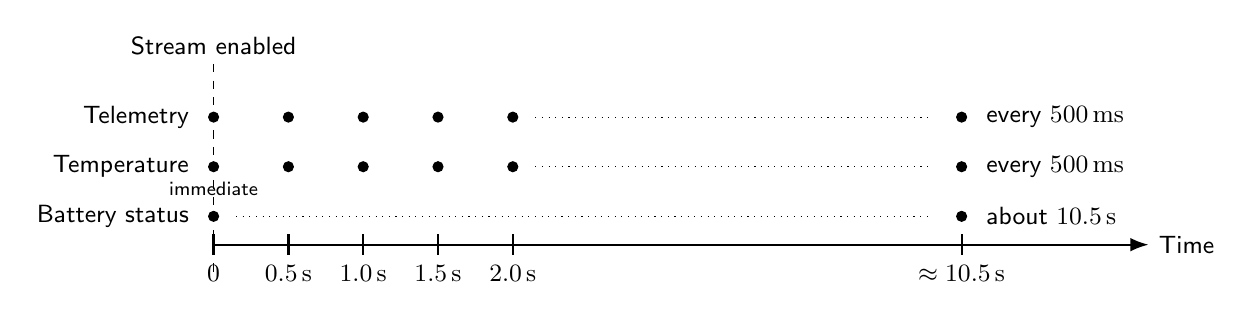
\begin{tikzpicture}[
		x=0.95cm,
		y=0.9cm,
		font=\small,
		axis/.style={-Latex, thick},
		tick/.style={thick}
		]
		% Time axis
		\draw[axis] (0,0) -- (12.5,0) node[right] {Time};
		
		% Tick marks
		\foreach \x/\label in {
			0/{\(0\)},
			1/{\(0.5\,\mathrm{s}\)},
			2/{\(1.0\,\mathrm{s}\)},
			3/{\(1.5\,\mathrm{s}\)},
			4/{\(2.0\,\mathrm{s}\)},
			10/{\(\approx 10.5\,\mathrm{s}\)}
		}{
			\draw[tick] (\x,0.15) -- (\x,-0.15) node[below] {\label};
		}
		
		% Stream enable marker
		\draw[dashed] (0,2.55) -- (0,-0.4);
		\node[above] at (0,2.55) {Stream enabled};
		
		% Telemetry row
		\node[left] at (-0.2,1.8) {Telemetry};
		\foreach \x in {0,1,2,3,4}{
			\draw[fill=black] (\x,1.8) circle (1.8pt);
		}
		\draw[dotted] (4.3,1.8) -- (9.6,1.8);
		\draw[fill=black] (10,1.8) circle (1.8pt);
		\node[right] at (10.2,1.8) {every \(500\,\mathrm{ms}\)};
		
		% Temperature row
		\node[left] at (-0.2,1.1) {Temperature};
		\foreach \x in {0,1,2,3,4}{
			\draw[fill=black] (\x,1.1) circle (1.8pt);
		}
		\draw[dotted] (4.3,1.1) -- (9.6,1.1);
		\draw[fill=black] (10,1.1) circle (1.8pt);
		\node[right] at (10.2,1.1) {every \(500\,\mathrm{ms}\)};
		
		% Battery row
		\node[left] at (-0.2,0.4) {Battery status};
		\draw[fill=black] (0,0.4) circle (1.8pt);
		\node[above] at (0,0.55) {\scriptsize immediate};
		\draw[dotted] (0.3,0.4) -- (9.6,0.4);
		\draw[fill=black] (10,0.4) circle (1.8pt);
		\node[right] at (10.2,0.4) {about \(10.5\,\mathrm{s}\)};
		
	\end{tikzpicture}
	\caption{WattMate notification timing after the telemetry stream has been enabled.}
	\label{fig:wattmate_streaming_timing}
\end{figure}

The notification timing is independent from the BLE connection interval. 
Connection events define when BLE packets can be exchanged, while the stream period defines when new application-level notification data are produced.


%--------------------------------------------------
% Simulation and PErformance Estimation
\newpage
\chapter{Simulation and Performance Estimation}
Before finalizing the manufacturing files, critical subsystems of the hardware design were simulated to validate mathematical sizing, verify layout choices and ensure compliance with the system's requirements.

\section{RF Antenna Design and Matching Network Tuning}
To guarantee reliable Bluetooth communication, the physical PCB layout of the antenna and its associated feedline was imported into Keysight Advanced Design System (ADS) and analyzed using the RFPro 3D electromagnetic (EM) simulation tool. This step was necessary because the performance results reported in the IFA antenna application report \cite{rf_ifa_ar} were obtained using a substrate thickness of \SI{1}{\milli\meter}, whereas the final design employs a different PCB stack-up. Since antenna characteristics are strongly influenced by substrate properties, including thickness and dielectric constant, a dedicated EM simulation was performed to accurately characterize the implemented RF structure, as shown in Figure~\ref{fig:ads_em_simulation}.

The simulation was used to extract the S-parameters of the RF section, with particular focus on the input reflection coefficient ($S_{11}$) and voltage standing wave ratio ($VSWR$), in order to evaluate the impedance matching between the MCU RF pin and the antenna. Based on the simulation results, the matching network component values were validated to closely match the nominal \SI{50}{\ohm} system impedance, thereby minimizing reflected power and maximizing power transfer to the antenna.

As shown in Figure~\ref{fig:s11_simulation}, the optimized design achieved an $S_{11}$ below \SI{-20}{\deci\bel} at the center frequency of \SI{2.45}{\giga\hertz}, corresponding to a very low reflected power level. Furthermore, the VSWR, reported in Figure~\ref{fig:vswr_simulation}, remained below 2 over an approximate bandwidth of \SI{200}{\mega\hertz}, fully covering the \SI{2.4}{\giga\hertz} ISM band and providing adequate tolerance against manufacturing variations and environmental detuning effects.

\begin{figure}[H]
    \centering
    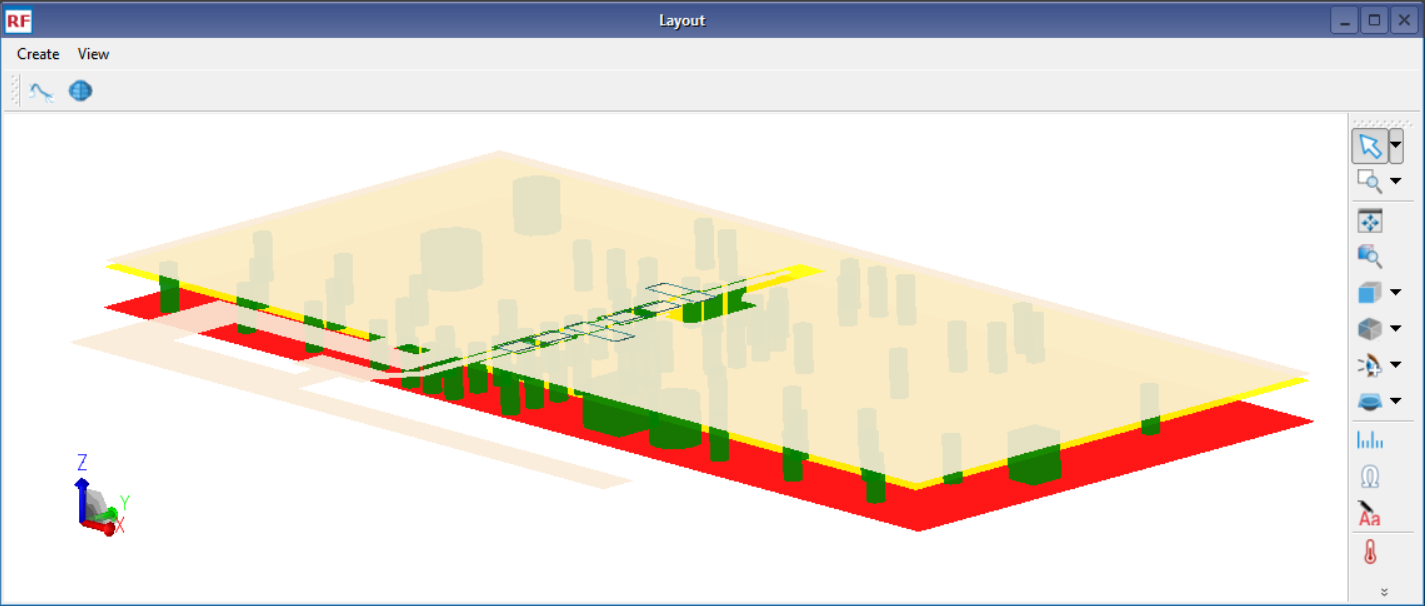
\includegraphics[width=0.9\linewidth]{figures/2_HW_figures/ads_em_simulation.png}
    \caption{3D EM simulation setup of the antenna and feedline in ADS RFPro.}
    \label{fig:ads_em_simulation}
\end{figure}

\begin{figure}[H]
    \centering
    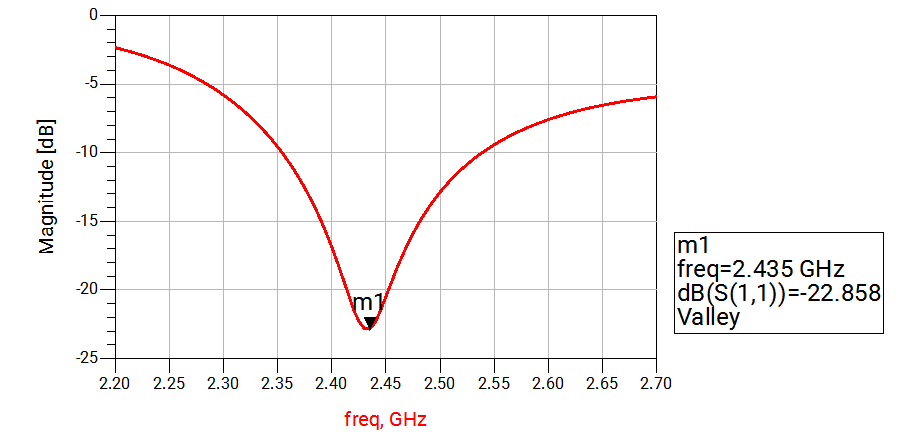
\includegraphics[width=0.85\linewidth]{figures/2_HW_figures/s11.png}
    \caption{Simulated $S_{11}$ (return loss) of the antenna and matching network obtained from simulation.}
    \label{fig:s11_simulation}
\end{figure}

\begin{figure}[H]
    \centering
    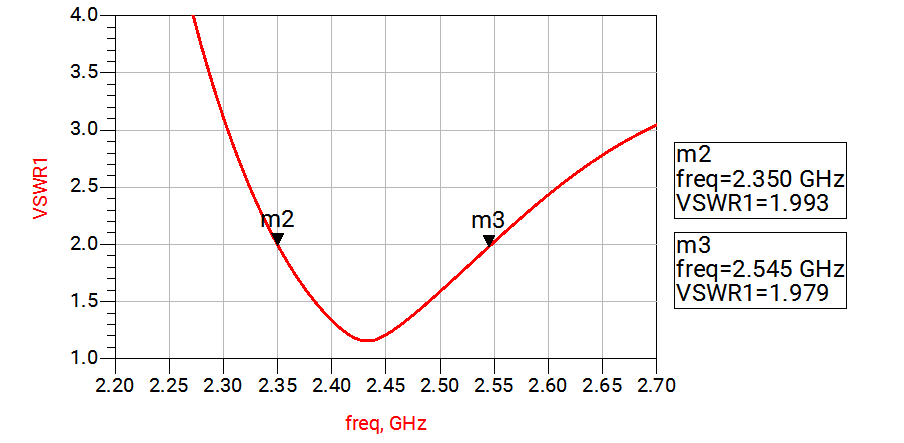
\includegraphics[width=0.85\linewidth]{figures/2_HW_figures/vswr.png}
    \caption{Simulated VSWR of the antenna and matching network showing impedance matching performance around 2.45 GHz.}
    \label{fig:vswr_simulation}
\end{figure}

\section{NTC Circuit with High-Side Enable Switch}
Temperature monitoring is performed using an NTC thermistor configured in a voltage divider. To satisfy the strict OFF-state power consumption requirement, this divider is not continuously powered. Instead, as explained in section~\ref{ntc}, it is driven by a high-side enable switch controlled by a microcontroller GPIO, ensuring current only flows during active ADC sampling.

A SPICE transient simulation was performed to analyze the dynamic response of this switching circuit (see Figure~\ref{fig:ntc_ltspice}). The simulation verified the turn-on settling time. Because the NTC node contains parasitic and filtering capacitance, the simulation determined the exact delay required between asserting the enable signal and triggering the ADC conversion. This ensures the analog voltage is sampled only after it has fully stabilized, guaranteeing temperature measurement accuracy without wasting power.

Based on the simulation results, the RC time constant of the sensing network was tuned to achieve a trade-off between settling time and noise filtering. In particular, the capacitance value of \SI{100}{\nano\farad} was selected to achieve attenuation higher than \SI{60}{\decibel} at the \SI{1.7}{\mega\hertz} dc-dc switching frequency, while still meeting the required acquisition timing defined by the system sampling constraints. In parallel, the gate pull-up resistor value of \SI{100}{\kilo\ohm} was chosen to ensure a fast enough turn-off of the sensing branch, preventing residual conduction during low-power operation while avoiding unnecessary quiescent current consumption.

The dynamic response analysis of the circuit allows the extraction of the settling time after the enable signal is asserted (see Figure~\ref{fig:ntc_spice_transient}). The measured rise time is approximately \SI{3}{\milli\second}, which defines the minimum safe acquisition window for the ADC conversion. This ensures that the sampled voltage is fully stabilized and free from transient effects. Based on this result, ON-time of \SI{5}{\milli\second} is chosen as a safety margin over the simulated settling time to guarantee robust operation under worst-case conditions.

\begin{figure}[H]
    \centering
    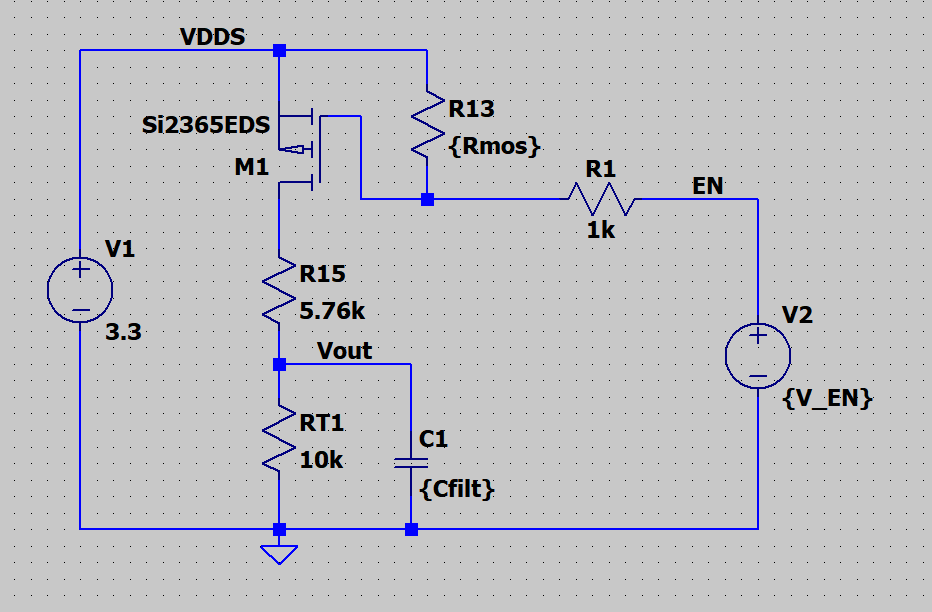
\includegraphics[width=0.75\textwidth]{figures/2_HW_figures/ntc_ltspice.png}
    \caption{LTspice simulation setup of the NTC sensing circuit used for transient and steady-state response analysis.}
    \label{fig:ntc_ltspice}
\end{figure}

\begin{figure}[H]
    \centering
    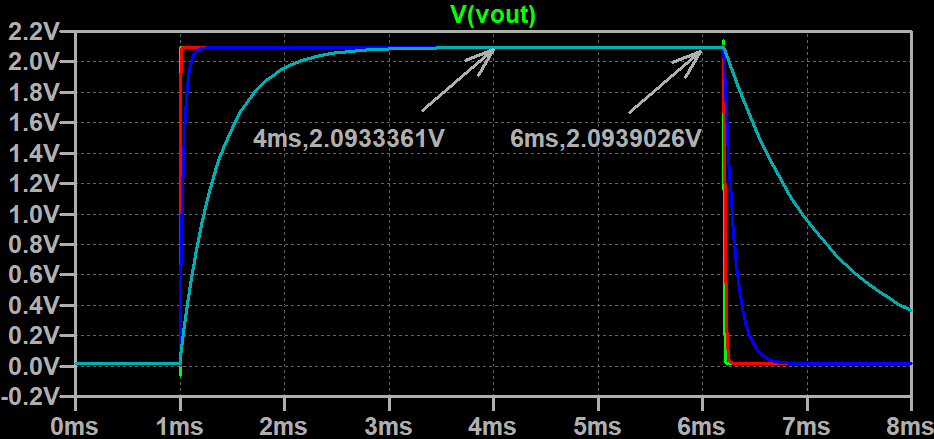
\includegraphics[width=0.75\textwidth]{figures/2_HW_figures/ntc_spice_transient.png}
    \caption{SPICE transient simulation of the NTC sensing circuit showing turn-on settling behavior.}
    \label{fig:ntc_spice_transient}
\end{figure}

After validation of the chosen component values in terms of dynamic response, an estimation of the power consumption was performed to quantify the benefit of the enable-controlled sensing circuit. The analysis compares the average power dissipation in both the always-on configuration and the duty-cycled implementation enabled by the MOSFET control stage.

The results show that, during a \SI{200}{\milli\second} period, the sensing network with the enable circuit dissipates an average power of \SI{5.55}{\micro\watt}, while in the always-enabled configuration the average power consumption increases to \SI{138}{\micro\watt}. This corresponds to an energy saving of around \SI{96}{\percent} over the defined duty cycle, significantly improving OFF-state battery life and supporting the system requirement defined in Requirement~\ref{req:pwr_battery}.



\section{System Power Consumption Evaluation}
\label{sec:system_power_consumption}

After the device selection and the definition of the main firmware timing parameters, the power consumption of WattMate can be estimated. 
This evaluation is used to verify the requirements related to the power consumption of the system regarding the ON-state efficiency and the idle battery life.

\subsection{Power Estimation Methodology}
\label{sec:power_estimation_methodology}

The total power dissipated by WattMate is evaluated by separating the losses introduced by the internal electronics from the power dissipated directly in the measured USB power path. 
For any given operating condition, the total dissipated power is modeled as:
\begin{equation}
	P_{WattMate} = P_{electronics} + P_{shunt} = (P_{components} + P_{DC/DC}) + P_{shunt}
\end{equation}

where \(P_{electronics}\) is the power required to supply the internal electronics of WattMate, while \(P_{shunt}\) is the power dissipated on the shunt resistor used to sense the USB bus current.

\(P_{electronics}\) can be further divided into the average power required by the internal circuitry and the average losses introduced by the power supply stage. 

\paragraph{Shunt dissipation.}
The shunt resistor is placed directly in the measured USB power path. 
Its power dissipation therefore depends on the current flowing through the monitored bus:
\begin{equation}
	P_{shunt} = I_{bus}^{2} \cdot R_{shunt}
\end{equation}

\paragraph{Component average power.}
The average consumption of each relevant electronic subsystem is estimated by assigning an active current, a sleep current, and a duty cycle. 
For each block, the average current is then computed as:
\begin{equation}
	\label{current_avg_formula}
	I_{avg} = D \cdot I_{ON} + \left(1-D\right) \cdot I_{sleep}
\end{equation}

where \(D\) is the fraction of time during which the block is ON in the considered operating condition.

The total average current required by the internal electronics is then obtained by summing the contribution of all powered blocks:
\begin{equation}
	I_{components} = \sum_k I_{avg,k}
\end{equation}

Assuming a regulated internal supply voltage \(V_{DD}\), the average power delivered to the components is:
\begin{equation}
	P_{components} = V_{DD} \cdot I_{components}
\end{equation}

The ON and sleep current values are defined once and then reused in the ON-state and idle evaluations. 
The duty cycles, instead, depend on the considered operating condition and are therefore evaluated separately for each scenario.

\paragraph{DC/DC converter losses.}
The DC/DC converter contribution is modeled as the sum of its quiescent power and conversion losses:
\begin{equation}
	P_{DC/DC} = P_{quiescent} + P_{loss}
\end{equation}

The quiescent term represents the power required by the converter control circuitry, while \(P_{loss}\) accounts for the finite conversion efficiency. 
Since the converter efficiency depends on the output current, \(P_{loss}\) is not estimated using only a single average current value. 
Instead, the detailed estimation is performed by defining a current profile and evaluating the converter efficiency in different current regions, as described in Section~\ref{sec:dcdc_loss_estimation}.

\subsection{Power Supply Loss Estimation}
\label{sec:dcdc_loss_estimation}

The DC/DC converter loss cannot be estimated accurately using only a single average output current, because the converter efficiency strongly depends on its output current. 
This effect is especially relevant at low load, where the efficiency of a switching converter can decrease significantly compared to its nominal value. 
For this reason, the duty cycles \(D\), defined for each electronic subsystem in each operating condition under evaluation, are used to define a current profile.

The current profile is built using a simple rule: each subsystem is considered ON at the start of the cycle and remains ON for a percentage of the cycle determined by its duty-cycle value. 
This current profile is still an approximation, because the complete dynamic behaviour of the device can only be verified experimentally, but it provides a more realistic design-stage estimate than assuming a constant output current.

This current profile is then used to evaluate the conversion loss by dividing it into representative output-current regions. 
For each region, the corresponding efficiency is extracted from the DC/DC converter datasheet. 
If \(P_{out,i}\), \(\eta_i\), and \(\alpha_i\) are respectively the output power, efficiency, and time fraction of region \(i\), the average conversion loss is computed as:
\begin{equation}
	P_{loss} = \sum_i \alpha_i \cdot P_{out,i} \cdot \left(\frac{1}{\eta_i} - 1\right)
\end{equation}

The quiescent power is evaluated under the worst-case input voltage:
\begin{equation}
	P_{quiescent} = V_{worst} \cdot I_{quiescent}
\end{equation}

The total DC/DC contribution is then:
\begin{equation}
	P_{DC/DC} = P_{quiescent} + P_{loss}
\end{equation}



\subsection{ON-state and Idle Currents for Subsystems}
\label{sec:on_idle_currents_subsystems}

After defining the duty cycle of each subsystem, the corresponding ON and idle currents must be assigned. 
These values are used to compute the average current contribution of each block according to the methodology introduced in Section~\ref{sec:power_estimation_methodology}.

When possible, the currents are taken directly from the component datasheets.

\paragraph{MCU core.}
The CC2640R2F datasheet models the ON MCU current as a fixed base contribution plus a frequency-dependent term~\cite{mcu_datasheet}. 
Since the firmware runs with a \(48\,\mathrm{MHz}\) system clock, the ON current used for the MCU core is:
\begin{equation}
	I_{MCU,ON} = I_{base} + I_{freq} \cdot f_{CPU}
	= 1.45\,\mathrm{mA} + 0.031\,\mathrm{mA/MHz} \cdot 48\,\mathrm{MHz}
	= 2.94\,\mathrm{mA}
\end{equation}

When the core is not ON, the standby current with retention is used as idle-state contribution~\cite{mcu_datasheet}:
\begin{equation}
	I_{MCU,idle} \simeq 1.1\,\mu\mathrm{A} = 0.0011\,\mathrm{mA}
\end{equation}

\paragraph{I\textsuperscript{2}C peripheral and pull-up resistors.}
The I\textsuperscript{2}C bus contribution is composed of two terms: the internal I\textsuperscript{2}C peripheral current of the MCU and the current dissipated by the external pull-up resistors on SDA and SCL.

The I\textsuperscript{2}C peripheral current is taken from the CC2640R2F datasheet~\cite{mcu_datasheet}:
\begin{equation}
	I_{I2C,periph,ON} = 12\,\mu\mathrm{A} = 0.012\,\mathrm{mA}
\end{equation}

The external pull-up resistors have a value of \(10\,\mathrm{k\Omega}\). 
When one I\textsuperscript{2}C line is driven low, the corresponding pull-up current is:
\begin{equation}
	I_{PU,line} = \frac{V_{DD}}{R_{PU}} = \frac{3.3\,\mathrm{V}}{10\,\mathrm{k\Omega}} = 0.33\,\mathrm{mA}
\end{equation}

During an active I\textsuperscript{2}C transfer, SCL is low for approximately half of the clock period, while the SDA level depends on the transmitted data. 
For a simple average estimate, the two bus lines are modeled as one equivalent pull-up resistor conducting during I\textsuperscript{2}C activity. 
The total ON current associated with the I\textsuperscript{2}C block is therefore:
\begin{equation}
	I_{I2C,ON} = I_{I2C,periph,ON} + I_{PU,I2C,ON}
	= 0.012\,\mathrm{mA} + 0.33\,\mathrm{mA}
	= 0.342\,\mathrm{mA}
\end{equation}

When the bus is inactive, both lines are pulled high and no static current flows through the pull-up resistors. 
The I\textsuperscript{2}C block is therefore considered idle outside the bus activity windows.

\paragraph{Other MCU peripheral contributions.}
Other MCU-side peripherals are grouped together. 
In the considered firmware configuration, this contribution includes two timers and the RF core idle contribution~\cite{mcu_datasheet}:
\begin{equation}
	I_{periph,ON} = 2 \cdot I_{timer} + I_{RFcore,idle}
	= 2 \cdot 113\,\mu\mathrm{A} + 237\,\mu\mathrm{A}
	= 463\,\mu\mathrm{A}
	= 0.463\,\mathrm{mA}
\end{equation}

This RF-core value represents the idle RF-core contribution and is kept separate from the BLE TX and RX radio currents, which are modeled independently.



\paragraph{External subsystems.}
The PAC1951 measurement sensor is set to the Normal Sampling Profile, defined in Section~\ref{PAC_Application_Task}, during ON-state measurement operation. 
In this configuration, the sensor samples one input channel at \(64\,\mathrm{SPS}\). 
During idle-state operation, the PAC1951 is set to the Idle Sampling Profile, also defined in Section~\ref{PAC_Application_Task}, where one input channel is sampled at \(8\,\mathrm{SPS}\). 
Given these operating conditions, the ON-state and idle-state currents of the PAC1951 are taken from the component datasheet~\cite{pac1951_datasheet}.

The NTC branch is powered only during temperature acquisition. 
Its ON current is computed from the circuit shown in Figure~\ref{fig:ntc_circuit}, using the thermistor value at \(25\,^\circ\mathrm{C}\), resulting in \(0.20\,\mathrm{mA}\)~\cite{ntc_datasheet}. 
When the NTC control MOSFET is disabled, the NTC branch is considered idle, and its current consumption is assumed to be zero.

The OLED display current is taken from the display datasheet for the reference condition of approximately \(50\%\) pixels ON~\cite{oled_datasheet}. 
When the display is disabled, its contribution is considered zero.

\paragraph{BLE radio currents.}
The BLE TX and RX currents are taken from the CC2640R2F datasheet~\cite{mcu_datasheet}. 
For the TX case, the \(+5\,\mathrm{dBm}\) value is used as a conservative estimate:
\begin{equation}
	I_{BLE,TX,ON} = 9.10\,\mathrm{mA}
\end{equation}

For RX activity, the ON-mode RX current is used:
\begin{equation}
	I_{BLE,RX,ON} = 6.10\,\mathrm{mA}
\end{equation}

The radio is considered idle outside the TX and RX activity windows estimated in Section~\ref{sec:standard_use_cycle}.

\begin{table}[H]
	\centering
	\small
	\caption{ON and idle current values used for the subsystem power estimate.}
	\label{tab:on_idle_currents_subsystems}
	\begin{tabular}{p{0.24\textwidth} p{0.18\textwidth} p{0.18\textwidth}}
		\toprule
		\textbf{Subsystem} & \textbf{\(I_{ON}\)} & \textbf{\(I_{idle}\)} \\
		\midrule
		MCU core &
		\(2.94\,\mathrm{mA}\) &
		\(0.0011\,\mathrm{mA}\) \\
		
		I\textsuperscript{2}C block &
		\(0.342\,\mathrm{mA}\) &
		\(0\,\mathrm{mA}\) \\
		
		Other MCU peripherals &
		\(0.463\,\mathrm{mA}\) &
		\(0\,\mathrm{mA}\) \\
		
		PAC1951 sensor &
		\(0.010\,\mathrm{mA}\) &
		\(0.005\,\mathrm{mA}\) \\
		
		NTC branch &
		\(0.200\,\mathrm{mA}\) &
		\(0\,\mathrm{mA}\) \\
		
		OLED display &
		\(32\,\mathrm{mA}\) &
		\(0\,\mathrm{mA}\) \\
		
		BLE TX &
		\(9.10\,\mathrm{mA}\) &
		\(0\,\mathrm{mA}\) \\
		
		BLE RX &
		\(6.10\,\mathrm{mA}\) &
		\(0\,\mathrm{mA}\) \\
		\bottomrule
	\end{tabular}
\end{table}













\subsection{ON-State Operating Efficiency}
\label{sec:operating_efficiency}

In this section, the power consumption of WattMate is evaluated under ON-state operating conditions, namely when non-negligible power is flowing through the USB power bus and WattMate is actively measuring the electrical state of the same bus.

The efficiency is evaluated under the worst-case bus operating point considered for the design:

\begin{equation}
	\label{eq:on_state_worst_case_conditions}
	V_{worst} = 21\,\mathrm{V}
	\qquad
	I_{worst} = 5\,\mathrm{A}
\end{equation}

These values represent the maximum voltage and current used to verify the ON-state efficiency requirement. 
They are used to compute the worst-case shunt dissipation, the worst-case monitored bus power, and the DC/DC quiescent contribution under maximum input voltage.

 

\paragraph{Standard Use Cycle}
\label{sec:standard_use_cycle}

The power consumption of WattMate in ON-state depends on the way the user interacts with the device. 
This is especially true for features related to the human interface, such as the OLED display and the BLE connection with the mobile application. 
For this reason, a standard use cycle is defined to estimate the average consumption in a repeatable way.

The standard use cycle is defined over \(1\,\mathrm{h}\) of operation and is summarized in Table~\ref{tab:standard_use_cycle}. 
It is not selected to minimize the estimated consumption, but to approximate the expected behaviour of a typical user.

\begin{table}[H]
	\centering
	\small
	\caption{Standard use cycle assumptions over \(1\,\mathrm{h}\) of operation.}
	\label{tab:standard_use_cycle}
	\begin{tabular}{p{0.22\textwidth} p{0.20\textwidth} p{0.48\textwidth}}
		\toprule
		\textbf{Interface} & \textbf{Frequency} & \textbf{Activation profile} \\
		\midrule
		OLED display &
		\(6\) activations/h &
		\(2\) activations last \(1\,\mathrm{min}\). 
		The remaining activations last only for the minimum firmware-defined ON time, corresponding to a quick check of the measured parameters. \\
		
		BLE mobile app &
		\(6\) sessions/h &
		Each application session lasts \(1\,\mathrm{min}\) on average. \\
		\bottomrule
	\end{tabular}
\end{table}

Based on this use cycle, each electronic subsystem is assigned a duty cycle \(D\), defined as the fraction of the reference cycle during which the subsystem is ON:

\begin{equation}
	D = \frac{t_{ON}}{t_{cycle}}
\end{equation}

where \(t_{ON}\) is the total ON-time of the subsystem during the cycle and \(t_{cycle}=1\,\mathrm{h}\).


\paragraph{PAC1951 sensor.}
The voltage and current sensor is considered always active during ON-state operation, because WattMate must continuously monitor the USB power path while the device is operating. 
Therefore, its duty cycle is:
\begin{equation}
	D_{VI} = 100\%
\end{equation}

\paragraph{Temperature sensor.}
The NTC temperature sensor is not continuously powered. It is enabled only during temperature acquisition, in order to reduce its average consumption. The temperature is sampled at \(5\,\mathrm{Hz}\). For each sample, the NTC supply MOSFET is enabled for the sensor settling time and for the ADC sampling time:
\begin{equation}
	t_{NTC,sample} = t_{settling} + t_{sampling}
	= 5\,\mathrm{ms} + 200\,\mu\mathrm{s}
	= 5.2\,\mathrm{ms}
\end{equation}

Since \(5\) samples are acquired every second, the total ON-time of the NTC over one second is:
\begin{equation}
	t_{NTC,ON/s} = 5 \cdot 5.2\,\mathrm{ms}
	= 26\,\mathrm{ms}
\end{equation}

The corresponding duty cycle is:
\begin{equation}
	D_{NTC} = \frac{26\,\mathrm{ms}}{1\,\mathrm{s}}
	= 2.6\%
\end{equation}

\paragraph{OLED display.}
The OLED display is ON only during the user interaction windows defined in the standard use cycle. 
Over \(1\,\mathrm{h}\), the total display ON-time is assumed to be \(4\,\mathrm{min}\). 
Therefore, the display duty cycle is:
\begin{equation}
	D_{OLED} = \frac{4\,\mathrm{min}}{60\,\mathrm{min}}
	= 6.67\%
\end{equation}

\paragraph{I\textsuperscript{2}C peripheral.}
The I\textsuperscript{2}C peripheral ON-time is estimated from the bus activity generated by the devices connected to the bus. 
In WattMate, the I\textsuperscript{2}C bus is used by the PAC1951 measurement sensor and by the OLED display. 
The bus operates at \(400\,\mathrm{kHz}\).

At protocol level, an I\textsuperscript{2}C communication is composed of a START condition, an address phase, one or more transferred bytes, and a STOP condition. 
A typical transaction can be represented as:
\begin{equation}
	\text{START} + \text{Address} + \text{R/W} + \text{ACK} + \text{Byte}_1 + \text{ACK} + \text{Byte}_2 + \text{ACK} + \cdots + \text{STOP}
\end{equation}

For the duty-cycle estimation, only SCL-clocked bits are counted. 
In particular, START, repeated START, and STOP conditions are not considered, because they are not transferred through a sequence of SCL clock pulses. 
They are bus conditions generated by specific transitions of the SDA line while SCL is high. 
This approximation slightly underestimates the real bus occupation time, because START and STOP conditions still require a finite setup and hold time. 
However, their contribution is small compared to the complete communication time, especially for multi-byte transfers such as sensor register reads and display framebuffer updates. 
Neglecting these conditions keeps the estimation simple and readable, while introducing only a small and acceptable approximation in the I\textsuperscript{2}C peripheral duty-cycle calculation.

Each data byte transferred on the bus is followed by one ACK / NACK bit, so each transferred byte occupies:
\begin{equation}
	N_{byte} = 8 + 1 = 9 \ \mathrm{bits}
\end{equation}

The I\textsuperscript{2}C address, communicated at the start of each communication, contains the \(7\)-bit I\textsuperscript{2}C slave address, the R/W bit, and the ACK bit, and so it occupies:
\begin{equation}
	N_{address} = 7 + 1 + 1 = 9 \ \mathrm{bits}
\end{equation}

For the PAC1951, commands are \(1\)-byte fields. 
Therefore, their communication occupies:
\begin{equation}
	N_{cmd}	= N_{address} + N_{byte} 
	= 9 + 9 = 18 \ \mathrm{bits}
\end{equation}
For the PAC1951, internal register addresses are \(1\)-byte fields. 
Therefore, a register-address byte occupies:
\begin{equation}
	N_{register}	= N_{byte}  = 9  \ \mathrm{bits}
\end{equation}

A register read of \(n\) data bytes is implemented as a combined write-read transaction. 
The master first writes the register address, then changes direction using a repeated START and reads the requested data:
\begin{equation}
	N_{read}(n)	= N_{address} + N_{register} + N_{address} + n \cdot N_{byte}
	= 9 + 9 + 9 + 9n 
	= 27 + 9n \ \mathrm{bits}
\end{equation}

During normal measurement operation, the PAC1951 is read at \(64\,\mathrm{Hz}\). 
The worst-case measurement update includes the reading of voltage, current, power, and energy accumulation registers.
The resulting bit count of each reading is reported in Table~\ref{tab:i2c_pac_bit_count}.
\begin{table}[H]
	\centering
	\small
	\caption{I\textsuperscript{2}C bit count for one PAC1951 measurement update.}
	\label{tab:i2c_pac_bit_count}
	\begin{tabularx}{0.78\textwidth}{@{}X l c c@{}}
		\toprule
		\textbf{Operation} & \textbf{Message Type} & \textbf{Data bytes} & \textbf{Bits} \\
		\midrule
		\texttt{REFRESH\_V} 	& Command	& --	& 18 \\
		Read average VBUS 		& Reg. Read	& 2		& 45 \\
		Read average VSENSE 	& Reg. Read	& 2		& 45 \\
		Read VPOWER 			& Reg. Read	& 4		& 63 \\
		\texttt{REFRESH\_V}		& Command	& --	& 18 \\
		Read accumulator count 	& Reg. Read	& 4		& 63 \\
		Read accumulator value 	& Reg. Read	& 7		& 90 \\
		\texttt{REFRESH} 		& Command	& --	& 18 \\
		\midrule
		Total 					& --		& -- 	& 360 \\
		\bottomrule
	\end{tabularx}
\end{table}

The measurement-related I\textsuperscript{2}C duty cycle is then computed as:
\begin{equation}
	D_{I\textsuperscript{2}C,meas}	= \frac{N_{bits,meas} \cdot f_{meas}}{f_{I\textsuperscript{2}C}}
	= \frac{360 \cdot 64}{400000} = 0.0576 = 5.76\%
\end{equation}

The OLED display also uses the I\textsuperscript{2}C bus when it is visible. 
In this case, the relevant operation is the full framebuffer refresh, because the display content is periodically updated while the screen is ON.

The OLED has a resolution of \(128 \times 64\) pixels and uses a framebuffer of \(1024\) bytes. 
The framebuffer is transferred in \(32\) chunks of \(32\) data bytes. 
Each chunk also includes one OLED control byte, so each framebuffer chunk transfers \(33\) bytes after the I\textsuperscript{2}C address phase.

Before sending the framebuffer data, an address-window command is transmitted to select the display memory region to be updated. 
This command transaction contains one OLED control byte and \(6\) command bytes, for a total of \(7\) transferred bytes. 
Using the same I\textsuperscript{2}C bit-count model defined above, the bit count of one full display refresh is:
\begin{equation}
	\begin{aligned}
		N_{display}
		& = \left(N_{address} + 7 \cdot N_{byte}\right) + 32 \cdot \left(N_{address} + 33 \cdot N_{byte}\right) \\ 
		& = \left(9 + 7 \cdot 9\right) + 32 \cdot \left(9 + 33 \cdot 9\right) = 72 + 9792 = 9864 \ \mathrm{bits}
	\end{aligned}
\end{equation}

When the display is visible, the framebuffer is refreshed every \(100\,\mathrm{ms}\), corresponding to an update frequency of \(10\,\mathrm{Hz}\). 
The I\textsuperscript{2}C duty cycle due to the OLED while the display is ON is therefore:
\begin{equation}
	D_{I\textsuperscript{2}C,OLED,ON}	= \frac{N_{display} \cdot f_{display}}{f_{I\textsuperscript{2}C}} 
	= \frac{9864 \cdot 10}{400000} 
	= 0.2466 
	= 24.66\%
\end{equation}

This value represents the I\textsuperscript{2}C bus usage only while the OLED is visible. 
In the standard use cycle, the display is ON for \(4\,\mathrm{min}\) over a \(60\,\mathrm{min}\) cycle, so the display visibility factor is:
\begin{equation}
	\alpha_{OLED}	= \frac{4\,\mathrm{min}}{60\,\mathrm{min}}
	= 0.0667
\end{equation}

The average OLED contribution to the I\textsuperscript{2}C duty cycle over the full standard use cycle is therefore:
\begin{equation}
	D_{I\textsuperscript{2}C,OLED,std}	= \alpha_{OLED} \cdot D_{I\textsuperscript{2}C,OLED,ON}
	= 0.0667 \cdot 24.66\%
	= 1.64\%
\end{equation}

The total I\textsuperscript{2}C peripheral ON-time used in the standard use cycle is then obtained by summing the PAC1951 measurement contribution and the average OLED contribution:
\begin{equation}
	D_{I\textsuperscript{2}C,std}	= D_{I\textsuperscript{2}C,meas} + D_{I\textsuperscript{2}C,OLED,std}
	= 5.76\% + 1.64\%
	= 7.40\%
\end{equation}

\paragraph{BLE radio.}
The BLE radio ON-time is estimated for the standard connected use cycle. 
In this condition, WattMate is assumed to be already connected to the mobile application, so advertising is not included in the BLE power estimate. 
The connection is kept active, Telemetry and Temperature notifications are periodically transmitted, and Battery Status notifications are neglected in the main calculation because they are sent at a much lower rate.

The BLE radio duty cycle is estimated using a simplified airtime model. 
The goal is not to reproduce the complete BLE timing at bit level, but to estimate the time during which the radio is active in TX and RX.

For a BLE data-channel packet, the on-air length is approximated as:
\begin{equation}
	N_{BLE} = N_{preamble} + N_{access} + N_{header} + N_{payload} + N_{CRC}
\end{equation}

where the fixed fields are \(1\,\mathrm{B}\) preamble, \(4\,\mathrm{B}\) access address, \(2\,\mathrm{B}\) Link Layer header, and \(3\,\mathrm{B}\) CRC. 
Therefore:
\begin{equation}
	N_{BLE} = 10 + N_{payload}
\end{equation}

The LE \(1\,\mathrm{Mbit/s}\) PHY is used for the estimate. 
This gives a conservative airtime with respect to LE 2M PHY, which is requested by WattMate but depends on the central device accepting the PHY update. 
At \(1\,\mathrm{Mbit/s}\), one bit corresponds to \(1\,\mu\mathrm{s}\), so the packet airtime is:
\begin{equation}
	t_{air} = 8 \cdot N_{BLE} \cdot 1 \ \mu\mathrm{s}
\end{equation}

For GATT notifications, the Link Layer payload includes the L2CAP header, the ATT Handle Value Notification fields, and the characteristic value:
\begin{equation}
	N_{payload} = N_{L2CAP} + N_{ATT} + N_{value}
\end{equation}

with \(N_{L2CAP}=4\,\mathrm{B}\) and \(N_{ATT}=3\,\mathrm{B}\). 
Therefore:
\begin{equation}
	N_{payload} = 7 + N_{value}
\end{equation}
During normal streaming, WattMate sends Telemetry and Temperature as two separate notifications every \(500\,\mathrm{ms}\). 
The Telemetry value is \(17\,\mathrm{B}\), while the Temperature value is \(2\,\mathrm{B}\). 
The corresponding airtimes are:
\begin{equation}
	t_{Telemetry} = 8 \cdot \left(10 + 7 + 17\right) = 272\,\mu\mathrm{s}
\end{equation}
\begin{equation}
	t_{Temperature} = 8 \cdot \left(10 + 7 + 2\right) = 152\,\mu\mathrm{s}
\end{equation}

The BLE connection is kept active even when no application data are exchanged. 
In this case, the central periodically opens connection events, and the peripheral must listen to them to maintain synchronization. 
For the power estimate, an empty connection event is modeled as one empty Link Layer packet received by WattMate and one empty Link Layer packet transmitted by WattMate.

An empty Link Layer packet has no payload:
\begin{equation}
	N_{empty} = 10\,\mathrm{B}
\end{equation}

and therefore:
\begin{equation}
	t_{empty} = 8 \cdot 10 = 80\,\mu\mathrm{s}
\end{equation}

The firmware requests a connection interval in the range \(15\,\mathrm{ms}\) to \(45\,\mathrm{ms}\), with peripheral latency equal to zero. 
For this estimate, the requested upper value is used as nominal connection period:
\begin{equation}
	T_{conn} = 45\,\mathrm{ms}
\end{equation}

The number of connection events per second is therefore:
\begin{equation}
	f_{conn} = \frac{1}{T_{conn}} = \frac{1}{45\,\mathrm{ms}} = 22.22\,\mathrm{Hz}
\end{equation}

Telemetry and Temperature are generated by the same stream update every \(500\,\mathrm{ms}\). 
Although they are sent as two separate notification packets, they are modeled as being transmitted within the same notification connection event. 
Therefore, the number of connection events carrying notification data is:
\begin{equation}
	N_{notifEvents/s} = 2
\end{equation}

To avoid double-counting the peripheral transmission, a notification connection event is modeled as replacing the empty TX packet with the Telemetry and Temperature notification packets. 
The remaining connection events are modeled as empty events:
\begin{equation}
	N_{emptyEvents/s} = f_{conn} - N_{notifEvents/s} = 22.22 - 2 = 20.22
\end{equation}

The BLE TX airtime per second is:
\begin{equation}
	\begin{aligned}
		t_{TX,BLE}
		&= N_{emptyEvents/s} \cdot t_{empty} + 2 \cdot t_{Telemetry} + 2 \cdot t_{Temperature} \\
		&= 20.22 \cdot 80\,\mu\mathrm{s} + 2 \cdot 272\,\mu\mathrm{s} + 2 \cdot 152\,\mu\mathrm{s} \\
		&= 2465.6\,\mu\mathrm{s/s}
	\end{aligned}
\end{equation}

The RX airtime includes one empty packet received in each empty connection event. 
For notification connection events, the model includes one received packet opening the event and one received empty response after each transmitted notification packet:
\begin{equation}
	\begin{aligned}
		t_{RX,BLE}
		&= N_{emptyEvents/s} \cdot t_{empty} + N_{notifEvents/s} \cdot 3t_{empty} \\
		&= 20.22 \cdot 80\,\mu\mathrm{s} + 2 \cdot 3 \cdot 80\,\mu\mathrm{s} \\
		&= 2097.6\,\mu\mathrm{s/s}
	\end{aligned}
\end{equation}

The resulting BLE radio duty cycles are:
\begin{equation}
	D_{BLE,TX} = \frac{2465.6\,\mu\mathrm{s}}{1\,\mathrm{s}} = 0.2466\%
\end{equation}
\begin{equation}
	D_{BLE,RX} = \frac{2097.6\,\mu\mathrm{s}}{1\,\mathrm{s}} = 0.2098\%
\end{equation}



\paragraph{MCU core and other peripherals.}
\label{par:on_state_mcu_core_peripherals}
The active duty cycle of the MCU core is difficult to estimate precisely without experimental measurements, because it depends on the RTOS scheduling behaviour, interrupt activity, driver execution time, and the time spent in low-power states. 
For this reason, a conservative design-stage estimate is used.

The activity explicitly estimated for the I\textsuperscript{2}C bus, BLE radio, and temperature sampling remains below the selected CPU activity margin. 
In addition, the MCU core is not expected to remain active during the full duration of peripheral or radio activity, since I\textsuperscript{2}C transfers are driver-managed, BLE timing-critical operations are handled by the BLE stack and RF core, and the NTC settling time does not require continuous CPU execution.

For the ON-state estimate, the MCU core active duty cycle is therefore assumed to be:
\begin{equation}
	D_{MCU} = 10\%
\end{equation}

This value is intentionally conservative and is expected to overestimate the real CPU activity during normal ON-state operation.

A similar design-stage assumption was adopted for the remaining on-chip peripherals. In the final firmware, peripherals such as timers and BLE/RF control subsystem are enabled and used by the RTOS tasks and TI drivers only when needed. However, without a detailed low-level execution trace or direct current measurements, the exact duty cycle of each internal peripheral cannot be determined reliably. Therefore, rather than introducing an overly detailed model with weak assumptions, a conservative usage factor of 10\% was assigned to the auxiliary peripheral contribution. This factor is intended to cover timer activity and BLE/RF control activity, while still reflecting that these blocks are event-driven and are not continuously active during normal ON-state operation. The BLE radio TX and RX currents are estimated separately using the airtime-based model, so this 10\% factor is not treated as an additional full-power radio duty cycle.

\paragraph{Average ON-State Component Consumption}
\label{sec:on_state_component_consumption}

Table~\ref{tab:active_component_consumption} summarizes the average current and power contribution of the main active components during the standard use cycle. 
The average current is computed using Equation~\ref{current_avg_formula}, while the average power is obtained from the regulated internal supply voltage \(V_{DD}=3.3\,\mathrm{V}\).

\begin{table}[H]
	\centering
	\small
	\setlength{\tabcolsep}{9pt}
	\caption{Average current and power contribution of the active components during the standard use cycle.}
	\label{tab:active_component_consumption}
	\begin{tabular}{@{}l r r c r r@{}}
		\toprule
		\textbf{Component} & \textbf{\(I_{ON}\)} & \textbf{\(I_{idle}\)} & \textbf{\(D\)} & \textbf{\(I_{avg}\)} & \textbf{\(P_{avg}\)} \\
		\midrule
		MCU core &
		\(2.94\,\mathrm{mA}\) &
		\(0.0011\,\mathrm{mA}\) &
		\(10\%\) &
		\(0.295\,\mathrm{mA}\) &
		\(0.97\,\mathrm{mW}\) \\
		
		I\textsuperscript{2}C block &
		\(0.342\,\mathrm{mA}\) &
		\(0\,\mathrm{mA}\) &
		\(7.40\%\) &
		\(0.025\,\mathrm{mA}\) &
		\(0.08\,\mathrm{mW}\) \\
		
		Other MCU peripherals &
		\(0.463\,\mathrm{mA}\) &
		\(0\,\mathrm{mA}\) &
		\(10\%\) &
		\(0.046\,\mathrm{mA}\) &
		\(0.15\,\mathrm{mW}\) \\
		
		BLE TX &
		\(9.10\,\mathrm{mA}\) &
		\(0\,\mathrm{mA}\) &
		\(0.2466\%\) &
		\(0.022\,\mathrm{mA}\) &
		\(0.07\,\mathrm{mW}\) \\
		
		BLE RX &
		\(6.10\,\mathrm{mA}\) &
		\(0\,\mathrm{mA}\) &
		\(0.2098\%\) &
		\(0.013\,\mathrm{mA}\) &
		\(0.04\,\mathrm{mW}\) \\
		
		PAC1951 sensor &
		\(0.010\,\mathrm{mA}\) &
		\(0.005\,\mathrm{mA}\) &
		\(100\%\) &
		\(0.010\,\mathrm{mA}\) &
		\(0.03\,\mathrm{mW}\) \\
		
		NTC branch &
		\(0.200\,\mathrm{mA}\) &
		\(0\,\mathrm{mA}\) &
		\(2.6\%\) &
		\(0.005\,\mathrm{mA}\) &
		\(0.02\,\mathrm{mW}\) \\
		
		OLED display &
		\(32\,\mathrm{mA}\) &
		\(0\,\mathrm{mA}\) &
		\(6.67\%\) &
		\(2.13\,\mathrm{mA}\) &
		\(7.04\,\mathrm{mW}\) \\
		\midrule
		Total &
		-- &
		-- &
		-- &
		\(2.55\,\mathrm{mA}\) &
		\(8.42\,\mathrm{mW}\) \\
		\bottomrule
	\end{tabular}
\end{table}



\paragraph{ON-State DC/DC Converter Loss Estimation}
\label{sec:on_state_dcdc_loss_estimation}

The DC/DC loss is evaluated using the method introduced in Section~\ref{sec:dcdc_loss_estimation}. 
The component power reported in Table~\ref{tab:active_component_consumption} represents the useful output power delivered by the converter to the internal electronics, while the converter loss depends on the efficiency at the corresponding output-current level.

Since the load current is not constant during the standard use cycle, the ON-state current profile is divided into three representative regions. 
For each region, a representative output current is used to extract the converter efficiency from the datasheet~\cite{max77597_datasheet}. 
The resulting current profile is shown in Figure~\ref{fig:dcdc_current_cycle}.
\begin{figure}[H]
	\centering
	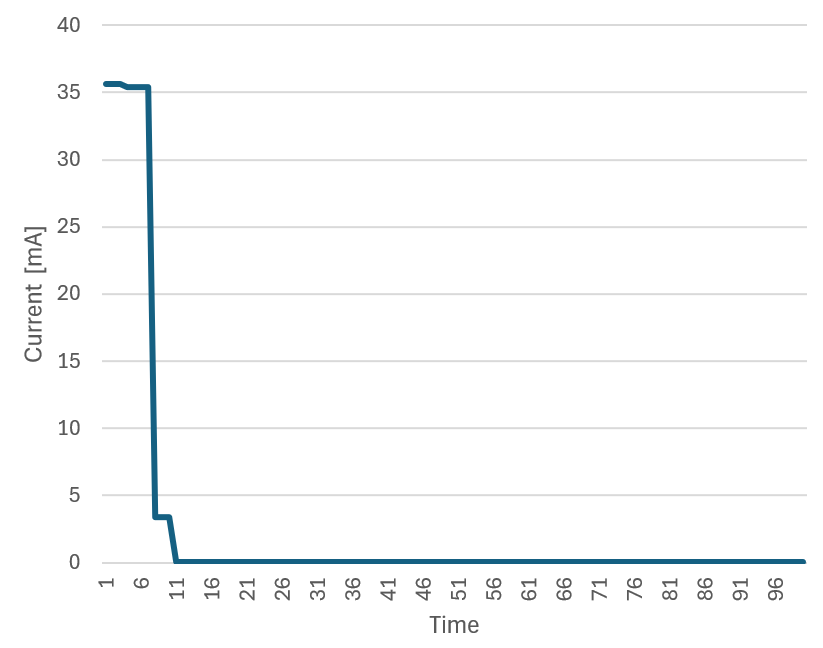
\includegraphics[width=0.55\textwidth]{figures/2_HW_figures/Standard_Cycle_Current_DC.png}
	\caption{Estimated DC/DC output current profile during the standard use cycle.}
	\label{fig:dcdc_current_cycle}
\end{figure}

The resulting loss estimation is reported in Table~\ref{tab:dcdc_loss_estimation}. 
The output power values are already averaged over the full standard use cycle. 
Therefore, for each region, the conversion loss is computed as:
\begin{equation}
	\label{eq:on_state_dcdc_region_loss}
	P_{loss,i} = P_{out,avg,i} \cdot \left(\frac{1}{\eta_i} - 1\right)
\end{equation}

\begin{table}[H]
	\centering
	\small
	\caption{DC/DC conversion loss estimation over the standard use cycle.}
	\label{tab:dcdc_loss_estimation}
	\begin{tabular}{@{}l c c c c c c@{}}
		\toprule
		\textbf{Region} & \textbf{\(I_{ref}\)} & \textbf{\(\eta\)} & \textbf{Time} & \textbf{\(I_{avg}\)} & \textbf{\(P_{out,avg}\)} & \textbf{\(P_{loss}\)} \\
		\midrule
		Low current &
		\(0.1\,\mathrm{mA}\) &
		\(70\%\) &
		\(90\%\) &
		\(0.01\,\mathrm{mA}\) &
		\(0.03\,\mathrm{mW}\) &
		\(0.01\,\mathrm{mW}\) \\
		
		Medium current &
		\(1\,\mathrm{mA}\) &
		\(80\%\) &
		\(10\%\) &
		\(2.59\,\mathrm{mA}\) &
		\(8.54\,\mathrm{mW}\) &
		\(2.13\,\mathrm{mW}\) \\
		
		High current &
		\(100\,\mathrm{mA}\) &
		\(85\%\) &
		\(0\%\) &
		\(0.00\,\mathrm{mA}\) &
		\(0.00\,\mathrm{mW}\) &
		\(0.00\,\mathrm{mW}\) \\
		\midrule
		Total &
		-- &
		-- &
		\(100\%\) &
		-- &
		-- &
		\(2.15\,\mathrm{mW}\) \\
		\bottomrule
	\end{tabular}
\end{table}

The total ON-state conversion loss is therefore:
\begin{equation}
	\label{eq:on_state_p_loss}
	P_{loss,ON} = \sum_i P_{loss,i} = 2.15\,\mathrm{mW}
\end{equation}

The quiescent power is evaluated under the worst-case input voltage, using the converter quiescent current reported in the datasheet~\cite{max77597_datasheet}:
\begin{equation}
	\label{eq:on_state_p_quiescent}
	P_{quiescent,ON} = V_{worst} \cdot I_{quiescent}
	= 21\,\mathrm{V} \cdot 1.1\,\mu\mathrm{A}
	\simeq 0.02\,\mathrm{mW}
\end{equation}

Using the DC/DC model defined in Section~\ref{sec:dcdc_loss_estimation}, the total DC/DC contribution during ON-state operation is:
\begin{equation}
	\label{eq:on_state_p_dcdc}
	P_{DC/DC,ON} = P_{quiescent,ON} + P_{loss,ON}
	= 0.02\,\mathrm{mW} + 2.15\,\mathrm{mW}
	= 2.17\,\mathrm{mW}
\end{equation}

The total power associated with the internal electronics is then:
\begin{equation}
	\label{eq:on_state_p_electronics}
	P_{electronics,ON} = P_{components,ON} + P_{DC/DC,ON}
	= 8.42\,\mathrm{mW} + 2.17\,\mathrm{mW}
	= 10.59\,\mathrm{mW}
\end{equation}


\paragraph{Power Distribution}
\label{sec:power_distribution}

Figure~\ref{fig:component_power_distribution} shows the relative contribution of the active electronics during the standard use cycle. 
The shunt power dissipation is not included in this chart, because it is much larger than the other contributions and would make the remaining component-level distribution unreadable.

\begin{figure}[H]
	\centering
	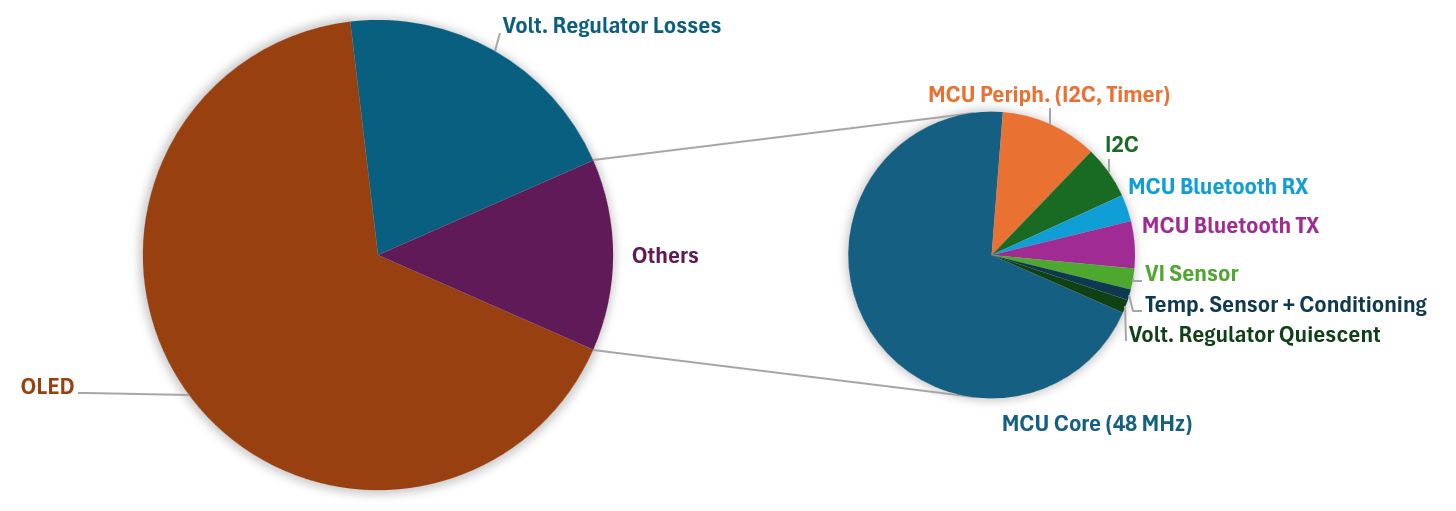
\includegraphics[width=0.95\textwidth]{figures/2_HW_figures/ON-state_Power_Distribution.png}
	\caption{Power distribution of the active electronics during the standard use cycle. The shunt dissipation is not included.}
	\label{fig:component_power_distribution}
\end{figure}

\paragraph{Shunt Power Dissipation}
\label{sec:shunt_power_dissipation}

The shunt resistor is placed in the measured USB power path. 
Its dissipation is therefore not related to the internal electronics duty cycle, but only to the current flowing through the monitored bus. 
Using the worst-case operating current, the shunt power is:
\begin{equation}
	\label{eq:on_state_p_shunt}
	P_{shunt,ON} = I_{worst}^{2} \cdot R_{shunt}
	= \left(5\,\mathrm{A}\right)^2 \cdot 0.01\,\Omega
	= 250\,\mathrm{mW}
\end{equation}


\subsubsection{Total ON-State Power Consumption and Efficiency}
\label{sec:total_on_state_power_consumption}

The total power dissipated by WattMate during ON-state operation is obtained by summing the shunt dissipation and the power required by the internal electronics. 
Using the internal electronics contribution computed in Equation~\ref{eq:on_state_p_electronics}:
\begin{equation}
	\label{eq:on_state_p_wattmate}
	P_{WattMate,ON} = P_{shunt,ON} + P_{electronics,ON}
	= 250\,\mathrm{mW} + 10.59\,\mathrm{mW}
	= 260.59\,\mathrm{mW}
\end{equation}

Under the worst-case operating condition of \(21\,\mathrm{V}\) and \(5\,\mathrm{A}\), the monitored bus power is:
\begin{equation}
	\label{eq:on_state_p_bus_worst}
	P_{bus,worst} = V_{worst} \cdot I_{worst}
	= 21\,\mathrm{V} \cdot 5\,\mathrm{A}
	= 105\,\mathrm{W}
\end{equation}

The corresponding ON-state efficiency is:
\begin{equation}
	\label{eq:on_state_efficiency}
	\eta_{ON}
	= \frac{P_{bus,worst}}{P_{bus,worst} + P_{WattMate,ON}}
	= \frac{105\,\mathrm{W}}{105\,\mathrm{W} + 0.26059\,\mathrm{W}}
	= 99.75\%
\end{equation}

This result satisfies the ON-state efficiency requirement, since the estimated efficiency is greater than \(99\%\) under the considered worst operating condition.



\subsection{Idle Consumption}
\label{sec:idle_consumption}

The idle consumption is evaluated using the same methodology introduced in Section~\ref{sec:power_estimation_methodology} and the same ON and idle current values defined in Section~\ref{sec:on_idle_currents_subsystems}. 
Only the duty cycles are changed, because the idle condition represents a different usage scenario.

In idle state, WattMate is powered and remains discoverable through BLE advertising, but no relevant power is assumed to flow through the monitored USB bus. 
Therefore, the shunt dissipation is considered null:
\begin{equation}
	\label{eq:idle_p_shunt}
	P_{shunt,idle} = 0
\end{equation}

The PAC1951 is kept in its idle sampling profile, while the I\textsuperscript{2}C bus, NTC branch, OLED display, and measurement-related peripherals are considered inactive. 
The only periodic active contribution is the BLE advertising transmission.

\paragraph{BLE advertising duty cycle.}
In idle state, WattMate remains discoverable through BLE advertising. 
The firmware uses a temporary fast advertising interval after startup or user interaction, but the steady idle condition is represented by the slow advertising interval:
\begin{equation}
	T_{adv,idle} = 1000\,\mathrm{ms}
\end{equation}

The idle advertising configuration is summarized in Table~\ref{tab:idle_ble_advertising_config}. 
Only the periodic advertising packets are included in the baseline idle estimate. 
Scan responses are not periodic and are transmitted only when an external scanner sends a scan request, so they are not included in the quiet-idle power calculation.

\begin{table}[H]
	\centering
	\small
	\caption{BLE advertising configuration used for the idle power estimate.}
	\label{tab:idle_ble_advertising_config}
	\begin{tabular}{@{}l l@{}}
		\toprule
		\textbf{Parameter} & \textbf{Idle advertising configuration} \\
		\midrule
		Advertising interval & \(1000\,\mathrm{ms}\) \\
		Advertising type & Legacy, connectable, scannable \\
		Advertising channels & Primary channels 37, 38, and 39 \\
		Advertising data length & \(13\,\mathrm{B}\) \\
		Advertising data content & BLE flags and complete local name \texttt{WattMate} \\
		\bottomrule
	\end{tabular}
\end{table}

The advertising packet airtime is estimated using the same simplified packet-level model adopted for the connected BLE radio estimate. 
For a legacy advertising packet, the on-air data include the preamble, access address, advertising header, advertiser address, advertising payload, and CRC:
\begin{equation}
	N_{adv} = 1\,\mathrm{B} + 4\,\mathrm{B} + 2\,\mathrm{B} + 6\,\mathrm{B} + 13\,\mathrm{B} + 3\,\mathrm{B}
	= 29\,\mathrm{B}
\end{equation}

Using the LE \(1\,\mathrm{Mbit/s}\) PHY, the airtime of one advertising packet is:
\begin{equation}
	t_{adv} = 8 \cdot N_{adv} \cdot 1\,\mu\mathrm{s}
	= 8 \cdot 29\,\mu\mathrm{s}
	= 232\,\mu\mathrm{s}
\end{equation}

Since one advertising event transmits the packet on the three primary advertising channels, the TX airtime of one idle advertising event is:
\begin{equation}
	t_{adv,event} = 3 \cdot t_{adv}
	= 3 \cdot 232\,\mu\mathrm{s}
	= 696\,\mu\mathrm{s}
\end{equation}

The resulting BLE advertising TX duty cycle is therefore:
\begin{equation}
	\label{eq:idle_ble_adv_duty}
	D_{BLE,TX,adv} = \frac{t_{adv,event}}{T_{adv,idle}}
	= \frac{696\,\mu\mathrm{s}}{1000\,\mathrm{ms}}
	= 0.0696\%
\end{equation}

The firmware uses the default \(0\,\mathrm{dBm}\) advertising TX power. 
The \(+5\,\mathrm{dBm}\) TX current reported in Table~\ref{tab:on_idle_currents_subsystems} is therefore a conservative upper-bound value for the idle estimate.


\paragraph{Idle duty-cycle summary.}
After defining the BLE advertising TX duty cycle, the complete set of idle duty-cycle assumptions can be summarized. 
A duty cycle equal to zero means that the corresponding subsystem is not actively used during idle operation and its idle current, defined in Table~\ref{tab:on_idle_currents_subsystems}, is applied.

The MCU core and the auxiliary MCU peripherals are assigned a conservative \(1\%\) active duty cycle. 
This margin accounts for the periodic wake-up activity required to manage BLE advertising and is selected with the same conservative approach discussed for the ON-state estimate in Paragraph~\ref{par:on_state_mcu_core_peripherals}.

\begin{table}[H]
	\centering
	\small
	\setlength{\tabcolsep}{7pt}
	\renewcommand{\arraystretch}{1.08}
	\caption{Idle-state duty-cycle assumptions.}
	\label{tab:idle_duty_cycle_summary}
	\begin{tabularx}{\textwidth}{@{}l c X@{}}
		\toprule
		\textbf{Subsystem} & \textbf{Duty cycle} & \textbf{Idle-state assumption} \\
		\midrule
		MCU core &
		\(1\%\) &
		Conservative margin for BLE advertising wake-up activity. \\
		
		I\textsuperscript{2}C block &
		\(0\%\) &
		No periodic I\textsuperscript{2}C traffic in idle. \\
		
		Other MCU peripherals &
		\(1\%\) &
		Conservative margin for timer and BLE/RF control activity. \\
		
		PAC1951 sensor &
		\(0\%\) &
		Idle sampling profile, so the idle current is applied. \\
		
		NTC branch &
		\(0\%\) &
		Temperature sensing branch disabled. \\
		
		OLED display &
		\(0\%\) &
		Display disabled. \\
		
		BLE TX &
		\(0.0696\%\) &
		Periodic legacy advertising transmission, from Equation~\ref{eq:idle_ble_adv_duty}. \\
		
		BLE RX &
		\(0\%\) &
		No connected-link RX activity in quiet idle. \\
		\bottomrule
	\end{tabularx}
\end{table}



\paragraph{Average Idle-State Component Consumption}
\label{sec:idle_component_consumption}

Table~\ref{tab:idle_component_consumption} summarizes the average current and power contribution of the subsystems that consume power during idle operation. 
The average current is computed using Equation~\ref{current_avg_formula}, while the average power is obtained from the regulated internal supply voltage \(V_{DD}=3.3\,\mathrm{V}\).

\begin{table}[H]
	\centering
	\small
	\setlength{\tabcolsep}{9pt}
	\caption{Average current and power contribution during idle operation.}
	\label{tab:idle_component_consumption}
	\begin{tabular}{@{}l r r c r r@{}}
		\toprule
		\textbf{Component} & \textbf{\(I_{ON}\)} & \textbf{\(I_{idle}\)} & \textbf{\(D\)} & \textbf{\(I_{avg}\)} & \textbf{\(P_{avg}\)} \\
		\midrule
		MCU core &
		\(2.94\,\mathrm{mA}\) &
		\(0.0011\,\mathrm{mA}\) &
		\(1\%\) &
		\(0.030\,\mathrm{mA}\) &
		\(0.10\,\mathrm{mW}\) \\
		
		Other MCU peripherals &
		\(0.463\,\mathrm{mA}\) &
		\(0\,\mathrm{mA}\) &
		\(1\%\) &
		\(0.005\,\mathrm{mA}\) &
		\(0.02\,\mathrm{mW}\) \\
		
		PAC1951 sensor &
		\(0.010\,\mathrm{mA}\) &
		\(0.005\,\mathrm{mA}\) &
		\(0\%\) &
		\(0.005\,\mathrm{mA}\) &
		\(0.02\,\mathrm{mW}\) \\
		
		BLE TX &
		\(9.10\,\mathrm{mA}\) &
		\(0\,\mathrm{mA}\) &
		\(0.0696\%\) &
		\(0.006\,\mathrm{mA}\) &
		\(0.02\,\mathrm{mW}\) \\
		\midrule
		Total &
		-- &
		-- &
		-- &
		\(0.046\,\mathrm{mA}\) &
		\(0.15\,\mathrm{mW}\) \\
		\bottomrule
	\end{tabular}
\end{table}


\subsubsection{Idle DC/DC Converter Loss Estimation}
\label{sec:idle_dcdc_loss_estimation}

The idle DC/DC loss is evaluated using the same procedure adopted for the ON-state case in Section~\ref{sec:on_state_dcdc_loss_estimation}. 
In idle operation, the load current remains very low for most of the time, but a small fraction of the cycle is still associated with a higher current level due to the periodic BLE advertising activity. 
For this reason, the idle current profile is divided into the same representative current regions used for the ON-state estimate.

The resulting loss estimation is reported in Table~\ref{tab:idle_dcdc_loss_estimation}. 
As in the ON-state case, the output power values are already averaged over the full idle cycle, and the conversion loss is computed from the efficiency of each current region.

\begin{table}[H]
	\centering
	\small
	\caption{DC/DC conversion loss estimation during idle operation.}
	\label{tab:idle_dcdc_loss_estimation}
	\begin{tabular}{@{}l c c c c c c@{}}
		\toprule
		\textbf{Region} & \textbf{\(I_{ref}\)} & \textbf{\(\eta\)} & \textbf{Time} & \textbf{\(I_{avg}\)} & \textbf{\(P_{out,avg}\)} & \textbf{\(P_{loss}\)} \\
		\midrule
		Low current &
		\(0.01\,\mathrm{mA}\) &
		\(40\%\) &
		\(99\%\) &
		\(0.01\,\mathrm{mA}\) &
		\(0.02\,\mathrm{mW}\) &
		\(0.03\,\mathrm{mW}\) \\
		
		Medium current &
		\(1\,\mathrm{mA}\) &
		\(80\%\) &
		\(1\%\) &
		\(0.03\,\mathrm{mA}\) &
		\(0.11\,\mathrm{mW}\) &
		\(0.03\,\mathrm{mW}\) \\
		
		High current &
		\(100\,\mathrm{mA}\) &
		\(85\%\) &
		\(0\%\) &
		\(0.00\,\mathrm{mA}\) &
		\(0.00\,\mathrm{mW}\) &
		\(0.00\,\mathrm{mW}\) \\
		\midrule
		Total &
		-- &
		-- &
		\(100\%\) &
		-- &
		-- &
		\(0.06\,\mathrm{mW}\) \\
		\bottomrule
	\end{tabular}
\end{table}

The quiescent power is evaluated using the same worst-case input voltage defined for the ON-state efficiency evaluation:
\begin{equation}
	\label{eq:idle_p_quiescent}
	P_{quiescent,idle} = V_{worst} \cdot I_{quiescent}
	= 21\,\mathrm{V} \cdot 1.1\,\mu\mathrm{A}
	\simeq 0.02\,\mathrm{mW}
\end{equation}

Using the DC/DC model defined in Section~\ref{sec:dcdc_loss_estimation}, the total DC/DC contribution during idle operation is:
\begin{equation}
	\label{eq:idle_p_dcdc}
	P_{DC/DC,idle} = P_{loss,idle} + P_{quiescent,idle}
	= 0.06\,\mathrm{mW} + 0.02\,\mathrm{mW}
	= 0.08\,\mathrm{mW}
\end{equation}

The total power associated with the internal electronics during idle operation is then:
\begin{equation}
	\label{eq:idle_p_electronics}
	P_{electronics,idle} = P_{components,idle} + P_{DC/DC,idle}
	= 0.15\,\mathrm{mW} + 0.08\,\mathrm{mW}
	= 0.23\,\mathrm{mW}
\end{equation}

\subsubsection{Total Idle-State Power Consumption}
\label{sec:total_idle_state_power_consumption}

In idle state, WattMate is powered, but no relevant current is assumed to flow through the monitored USB power bus. 
Since the idle shunt dissipation has already been defined as zero in Equation~\ref{eq:idle_p_shunt}, the total idle-state power consumption is only given by the internal electronics contribution:
\begin{equation}
	\label{eq:idle_p_wattmate}
	P_{WattMate,idle} = P_{electronics,idle} + P_{shunt,idle}
	= 0.23\,\mathrm{mW} + 0\,\mathrm{mW}
	= 0.23\,\mathrm{mW}
\end{equation}

Figure~\ref{fig:idle_power_distribution} reports the distribution of the idle-state power consumption. 
As for the ON-state distribution in Figure~\ref{fig:component_power_distribution}, the chart separates the main contributors and highlights the smaller contributions in a secondary pie chart.

\begin{figure}[H]
	\centering
	\includegraphics[width=0.95\textwidth]{figures/2_HW_figures/IDLE-State_Power_Distribution.png}
	\caption{Power distribution of WattMate during idle-state operation.}
	\label{fig:idle_power_distribution}
\end{figure}


\paragraph{Idle battery endurance.}
Considering a battery energy of \(32\,\mathrm{Wh}\), the ideal idle endurance is estimated as:
\begin{equation}
	\label{eq:idle_endurance_hours}
	t_{idle} = \frac{E_{battery}}{P_{WattMate,idle}}
	= \frac{32\,\mathrm{Wh}}{0.00023\,\mathrm{W}}
	\simeq 1.39 \cdot 10^{5}\,\mathrm{h}
\end{equation}

which corresponds to:
\begin{equation}
	\label{eq:idle_endurance_days}
	t_{idle,days} = \frac{t_{idle}}{24}
	= \frac{1.39 \cdot 10^{5}}{24}
	\simeq 5.80 \cdot 10^{3}\,\mathrm{days}
\end{equation}

This value represents an ideal electronics-only endurance. 
In a real product, the effective long-term idle lifetime would also be limited by battery self-discharge and by leakage currents not included in this design-stage estimate.
%--------------------------------------------------

% Tests
\chapter{Performance and Validation}

\section{Test Setup}
To ensure both precise laboratory validation and real-world functional verification, the device was subjected to four distinct testing configurations:

\begin{description}
    \item[Setup 1: Wall Adapter (Unloaded)] A standard commercial USB Type-C wall adapter was connected to the WattMate input port, with the output port left unconnected. This setup was used to verify the initial boot sequence without load-induced voltage drops.
    
    \item[Setup 2: Wall Adapter to Smartphone] A wall adapter was connected to the input, and a commercial smartphone was connected to the output port. This configuration represents the primary real-world use case of the device, allowing for dynamic load testing as the phone's internal battery management system negotiates power.
    
    \item[Setup 3: DC Power Supply (Unloaded)] A precision laboratory DC power supply was injected into the input port, with the output floating. This setup provided highly regulated, noise-free power and allowed for manual, precise adjustments of the input voltage to test the system's operational boundaries.
    
    \item[Setup 4: DC Power Supply to Resistive Load] The laboratory DC power supply drove the input, while a resistive load was connected to the output. This configuration allowed for strict, controlled current draws to test the thermal dissipation of the PCB and the linearity of the analog current sensing circuit.
\end{description}



\begin{figure}[H]
\centering

% ===================== SETUP 1 =====================
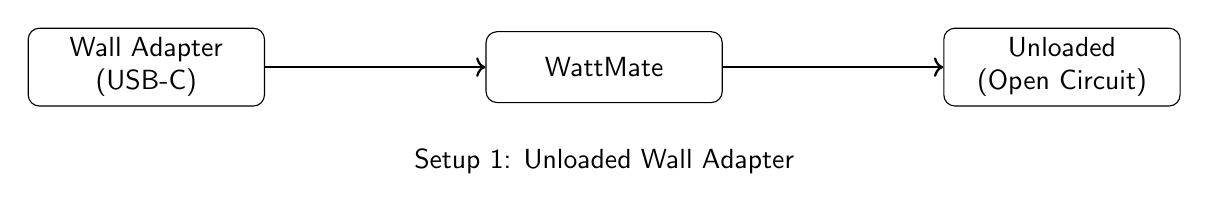
\begin{tikzpicture}[
    block/.style={draw, rounded corners, minimum width=3cm, minimum height=0.9cm, align=center},
    arrow/.style={->, thick}
]
\node[block] (in) {Wall Adapter\\(USB-C)};
\node[block, right=2.8cm of in] (dev) {WattMate};
\node[block, right=2.8cm of dev] (out) {Unloaded\\(Open Circuit)};

\draw[arrow] (in) -- (dev);
\draw[arrow] (dev) -- (out);

\node at ($(in)!0.5!(out) + (0,-1.2)$) {Setup 1: Unloaded Wall Adapter};

\end{tikzpicture}

\vspace{0.6cm}

% ===================== SETUP 2 =====================
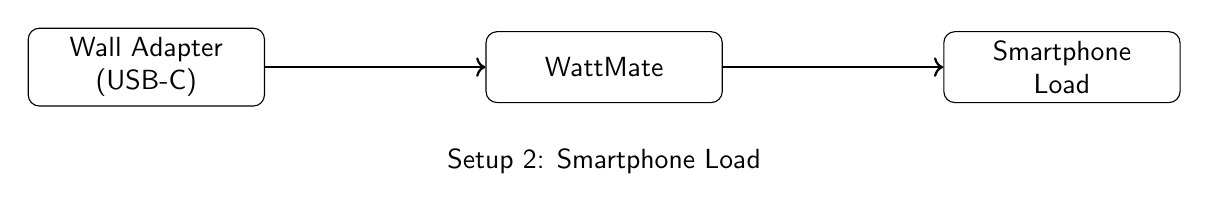
\begin{tikzpicture}[
    block/.style={draw, rounded corners, minimum width=3cm, minimum height=0.9cm, align=center},
    arrow/.style={->, thick}
]
\node[block] (in) {Wall Adapter\\(USB-C)};
\node[block, right=2.8cm of in] (dev) {WattMate};
\node[block, right=2.8cm of dev] (out) {Smartphone\\Load};

\draw[arrow] (in) -- (dev);
\draw[arrow] (dev) -- (out);

\node at ($(in)!0.5!(out) + (0,-1.2)$) {Setup 2: Smartphone Load};

\end{tikzpicture}

\vspace{0.6cm}

% ===================== SETUP 3 =====================
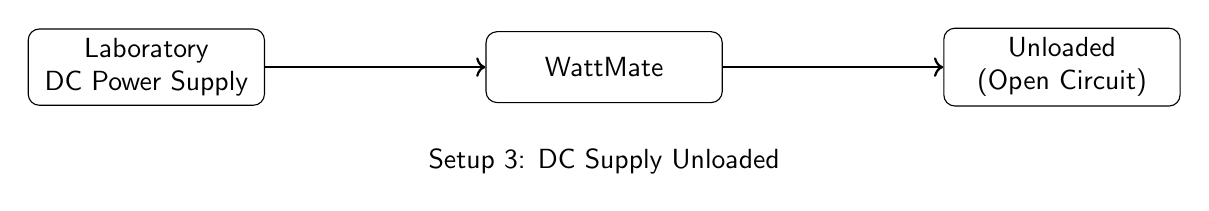
\begin{tikzpicture}[
    block/.style={draw, rounded corners, minimum width=3cm, minimum height=0.9cm, align=center},
    arrow/.style={->, thick}
]
\node[block] (in) {Laboratory\\DC Power Supply};
\node[block, right=2.8cm of in] (dev) {WattMate};
\node[block, right=2.8cm of dev] (out) {Unloaded\\(Open Circuit)};

\draw[arrow] (in) -- (dev);
\draw[arrow] (dev) -- (out);

\node at ($(in)!0.5!(out) + (0,-1.2)$) {Setup 3: DC Supply Unloaded};

\end{tikzpicture}

\vspace{0.6cm}

% ===================== SETUP 4 =====================
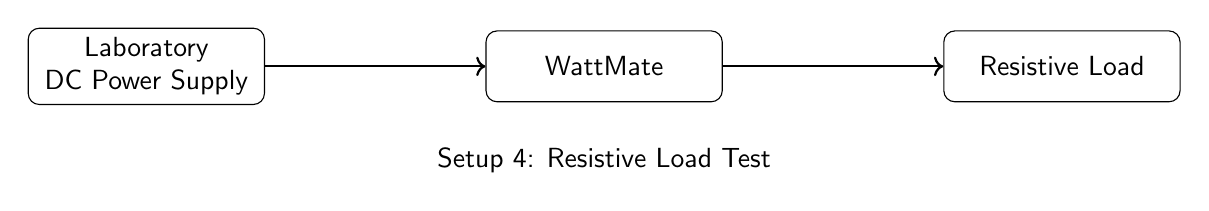
\begin{tikzpicture}[
    block/.style={draw, rounded corners, minimum width=3cm, minimum height=0.9cm, align=center},
    arrow/.style={->, thick}
]
\node[block] (in) {Laboratory\\DC Power Supply};
\node[block, right=2.8cm of in] (dev) {WattMate};
\node[block, right=2.8cm of dev] (out) {Resistive Load};

\draw[arrow] (in) -- (dev);
\draw[arrow] (dev) -- (out);

\node at ($(in)!0.5!(out) + (0,-1.2)$) {Setup 4: Resistive Load Test};

\end{tikzpicture}

\caption{Test setups used for validation of the WattMate system under different input sources and load conditions.}
\label{fig:wattmate_setups}
\end{figure}



\section{Test Results}

\subsection{Initial Working Verification (\SI{5}{\volt})}
The initial functional verification was performed using both Setup 1 and Setup 3, providing a standard \SI{5}{\volt} VBUS input. In both scenarios, the MAX77597 step-down converter successfully activated, providing a stable \SI{3.260}{\volt} logic supply. The MCU successfully completed its boot sequence, initialized the $I^2C$ bus and the BLE communication, allowing external connection through the mobile application. However, under specific operating conditions, the OLED display failed to initialize. This behavior, alongside the deviations observed on the \SI{3.3}{\volt} logic rail, is discussed in detail in Section~\ref{problems}.

\subsection{Input DC Voltage Sweep (\SI{4}{\volt} to \SI{30}{\volt})}
To validate the high-voltage resilience of the system and the wide-input capabilities of the DC-DC converter, an input voltage sweep was performed using Setup 3. The DC power supply was slowly ramped from \SI{4}{\volt} up to a maximum over-voltage state of \SI{30}{\volt}. 
\par
Throughout the entire sweep, the \SI{3.3}{\volt} rail remained perfectly stable. Furthermore, the average voltage readings reported by the PAC1951 sensor via the MCU precisely matched the laboratory equipment's output, confirming that the sensing stage was implemented and initialized correctly. However, the recorded data exhibited a superimposed noise higher than expected, resulting in a flactuating reading.

\subsection{High-Current Load Testing (Up to \SI{3}{\ampere})}
Current sensing accuracy and thermal stability were validated using Setup 4. By adjusting the resistive load, the current drawn through the VBUS line was steadily increased in increments up to \SI{3}{\ampere}, reaching the limit of the DC power supply available in the laboratory. 
\par
The physical VBUS polygon pours and via arrays easily handled the current without significant thermal gradients. The current measurements demonstrated good linearity from \SI{100}{\milli\ampere} up to \SI{3}{\ampere}. AS for the voltage reading, the recorded data exhibited a superimposed noise higher than expected, resulting in a flactuating reading.

\subsection{State of Charge (SoC) Estimation}
The pseudo-real State of Charge (SoC) estimation was validated using Setup 2 by charging a smartphone from a depleted state. To validate the implemented algorithm and the charging cycle information management, the end-of-cycle energy threshold was temporarily reduced from its nominal value. This modification allowed multiple charging cycles to be completed in a shorter time, enabling repetitive testing without waiting for a full smartphone charge and subsequent discharge.

The system successfully tracked the passing energy throughout the entire cycle, with the OLED display accurately reflecting the real-time state of charge as the smartphone transitioned from charging to discharging cycles.

% Optional: Add a figure here if you have a plot of the voltage sweep or SoC curve!
% \begin{figure}[H]
%     \centering
%     \includegraphics[width=0.7\textwidth]{figures/soc_curve.png}
%     \caption{Measured State of Charge (SoC) estimation over time during the smartphone charging test (Setup 2).}
%     \label{fig:soc_test}
% \end{figure}

\section{Problems and Troubleshooting}\label{problems}

While the overall architecture performed as expected, several issues were identified during the hardware bring-up and validation phases:

\subsection{Measurement Noise}

During validation testing, the voltage, current, and temperature measurements exhibited a higher noise level than initially expected. Investigation revealed that the primary source of the issue was excessive ripple on the \SI{3.3}{\volt} power supply rail. Although the DC-DC converter was designed to operate at a switching frequency of \SI{1.7}{\mega\hertz}, its power-saving skip mode had been enabled. Under the relatively low load conditions of the system, the regulator automatically reduced its switching activity to improve efficiency and minimize switching losses. As a consequence, the output ripple became strongly non-stationary, exhibiting a dynamically varying periodic behavior.

In particular, the ripple frequency was observed to fluctuate between approximately \SI{350}{\hertz} and \SI{2.5}{\kilo\hertz}, depending on the instantaneous load condition and burst switching activity of the regulator. This behavior results in a non-constant ripple period, as shown in Figure~\ref{fig:dc_dc_ripple_dynamic}, which increases spectral content in the low-frequency range and makes filtering significantly less effective compared to a fixed-frequency switching regime.

The selected output filter inductor and capacitor, had been optimized for nominal operating conditions and were therefore not sufficiently effective under this variable-frequency skip-mode operation. This resulted in an output ripple of approximately \SI{120}{\milli\volt} peak-to-peak, which coupled into the analog measurement circuitry and degraded the accuracy of sensor readings.

Figure~\ref{fig:dc_dc_ripple_dynamic} shows the measured dynamic ripple behavior on the \SI{3.3}{\volt} rail, highlighting the non-constant switching period.

\begin{figure}[H]
    \centering
    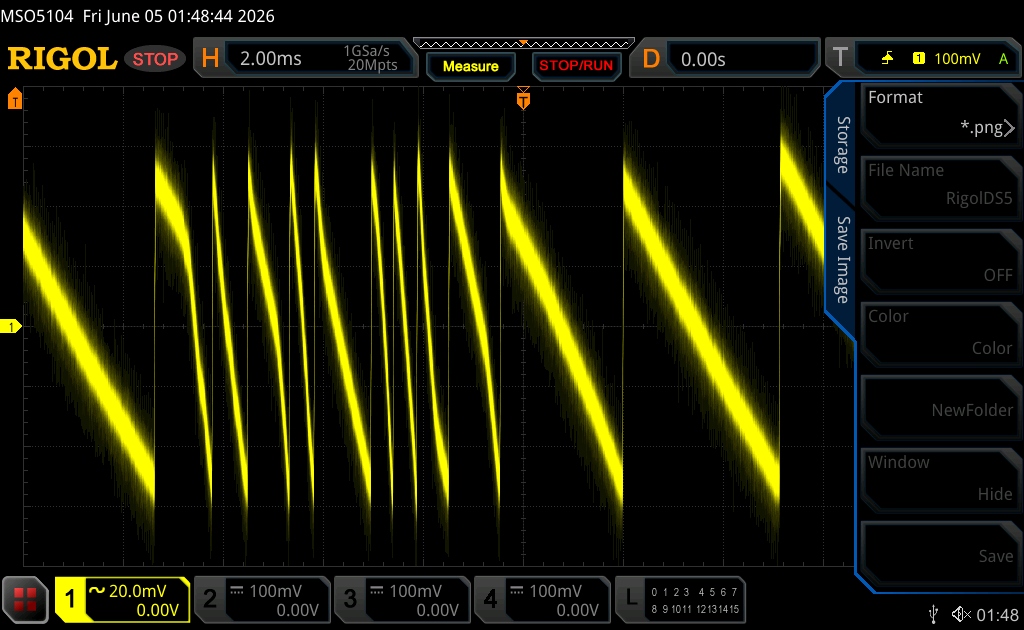
\includegraphics[width=0.85\textwidth]{figures/rail_ripple.png}
    \caption{Measured \SI{3.3}{\volt} rail ripple showing dynamic skip-mode behavior with non-constant switching frequency.}
    \label{fig:dc_dc_ripple_dynamic}
\end{figure}
    
\subsection{OLED Display Startup Issue}

During certain operating conditions, the OLED display failed to initialize correctly at board power-up. Specifically, the display remained off and did not enter its normal operating state. The issue was traced to an incorrect generation of the internal high-voltage rail required by the display driver.

The OLED module integrates an internal charge pump that generates the \SI{7.5}{\volt} supply required for display operation, using the external logic supply rail as its input. This supply is nominally specified in the range of \SIrange{3.3}{4.2}{\volt}. Because of the DC-DC buck controller regulation error, this supply rail was slightly degraded, measuring approximately \SI{3.26}{\volt}, and was further affected by significant introduced \SI{120}{\milli\volt} ripple (as described in the previous subsection). This combination of reduced DC level and superimposed ripple caused the SSD1306 charge pump to intermittently fail its start-up condition. In practice, the input voltage fell close to or below the internal start-up threshold of the charge pump control circuitry, preventing the generation of the required \SI{7.5}{\volt} internal supply. As a result, the display driver remained inactive and the OLED did not turn on. The issue was not observed when the system was powered from a clean \SI{3.3}{\volt} LDO-regulated supply. Under these conditions, the SSD1306 consistently succeeded in enabling the charge pump and correctly generating the internal high-voltage rail, resulting in reliable display initialization.

An additional dependency was observed on the system power-down state. When the board was powered after a sufficiently long off-time, allowing the discharge of the onboard capacitors, the initial power-up transient was sufficient to trigger correct charge pump start-up. However, during consecutive power cycles performed in quick succession, residual charge on the supply network reduced the effective startup transient amplitude. In these cases, the voltage step was insufficient to overcome the unknown internal start-up threshold of the charge pump, leading again to failure in generating the \SI{7.5}{\volt} rail and consequently preventing display activation.

\section{Possible Solutions and Future Improvements}

Since both observed issues are related to the quality and level of the \SI{3.3}{\volt} power rail, a single design modification can address them simultaneously. In particular, the system must satisfy two competing requirements: providing a clean, low-noise supply for the microcontroller and analog sensing circuitry, while also ensuring a sufficiently high input voltage for reliable startup of the OLED module internal charge pump.

To meet these constraints, the existing DC-DC buck converter is retained in order to preserve high overall efficiency during operation. However, its output voltage is adjusted slightly above the nominal \SI{3.3}{\volt} level, for example to \SI{3.5}{\volt} or \SI{3.6}{\volt}. This increase ensures that, even in the presence of ripple and transient voltage drops, the OLED driver input remains above the minimum start-up threshold required for correct charge pump operation, thereby improving initialization robustness.

A secondary low-dropout (LDO) regulator is then used to derive a clean and stable \SI{3.3}{\volt} rail from this intermediate voltage. Given the small voltage difference between \SI{3.5}{\volt}--\SI{3.6}{\volt} and \SI{3.3}{\volt}, the LDO operates with minimal power dissipation while effectively attenuating the switching ripple introduced by the buck converter. This configuration ensures a low-noise supply for sensitive analog and digital subsystems, including the MCU, the PAC1951 sensing circuitry, and the NTC temperature measurement network.

As a trade-off, the introduction of the LDO regulator introduces an additional power dissipation stage, leading to a reduction in overall system efficiency. Although the OLED display is not powered through the LDO, the regulator still supplies a portion of the system load which draw a few milliamperes under normal operation. The resulting voltage drop between the intermediate rail and the regulated \SI{3.3}{\volt} output leads to continuous power dissipation across the LDO. Nevertheless, this efficiency penalty is considered acceptable, as the affected currents are relatively low and the overall impact on the system power budget remains limited. In return, the proposed architecture significantly improves supply integrity, reduces ripple on sensitive analog circuitry, and increases the robustness of the OLED charge pump startup.

\begin{figure}[H]
\centering
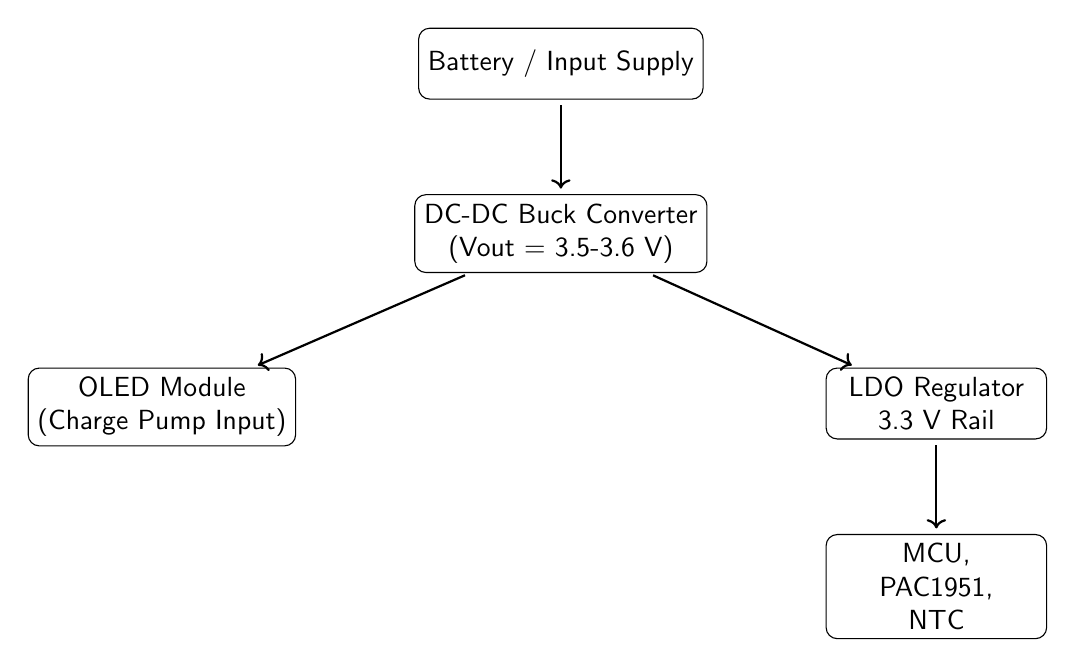
\begin{tikzpicture}[
    node distance=1.2cm and 1.5cm,
    block/.style={draw, rounded corners, minimum width=2.8cm, minimum height=0.9cm, align=center},
    arrow/.style={->, thick}
]

% Nodes
\node[block] (vin) {Battery / Input Supply};

\node[block, below=of vin] (buck) {DC-DC Buck Converter\\(Vout = 3.5-3.6 V)};

\node[block, below left=of buck] (oled) {OLED Module\\(Charge Pump Input)};

\node[block, below right=of buck] (ldo) {LDO Regulator\\3.3 V Rail};

\node[block, below=of ldo] (v33) {MCU, \\PAC1951,\\ NTC};

% Connections (shortened arrows)
\draw[arrow, shorten >=2pt, shorten <=2pt] (vin) -- (buck);

\draw[arrow, shorten >=2pt, shorten <=2pt] (buck) -- (oled);

\draw[arrow, shorten >=2pt, shorten <=2pt] (buck) -- (ldo);

\draw[arrow, shorten >=2pt, shorten <=2pt] (ldo) -- (v33);

\end{tikzpicture}
\caption{Proposed power supply architecture with boosted buck output and post-regulation LDO for low-noise 3.3 V rail.}
\label{fig:power_supply_tree}
\end{figure}


%\section{Compliance and Certifications}

%--------------------------------------------------

% Mechanical
\chapter{Mechanical Design and \\Integration}

\section{Enclosure Overview}
The system is housed within a compact, custom-designed two-part enclosure. It should be noted that this mechanical design represents the \textit{external monitor configuration} of the system, tailored specifically for its use as a standalone, inline diagnostic tool. For future deployments where the measurement and communication circuitry are integrated directly into the internal architecture of a commercial power bank, the external case will no longer apply. In such integrated configurations, the final enclosure and physical constraints will be defined entirely by the customer (the power bank manufacturer) to align with their specific industrial design.

\subsection{Assembly Components}
The physical construction of the device is achieved through a multi-part mechanical assembly. The complete system comprises the custom two-part plastic enclosure (top and bottom covers), a dedicated clear screen cover to protect the display, the fully populated Printed Circuit Board (PCB), and the required mounting hardware. Table~\ref{tab:mech_components} details each of these individual physical components as illustrated in the exploded view of the system (Figure~\ref{fig:mech_exploded}).

\begin{figure}[H]
    \centering
    % Update the filename/path if necessary
    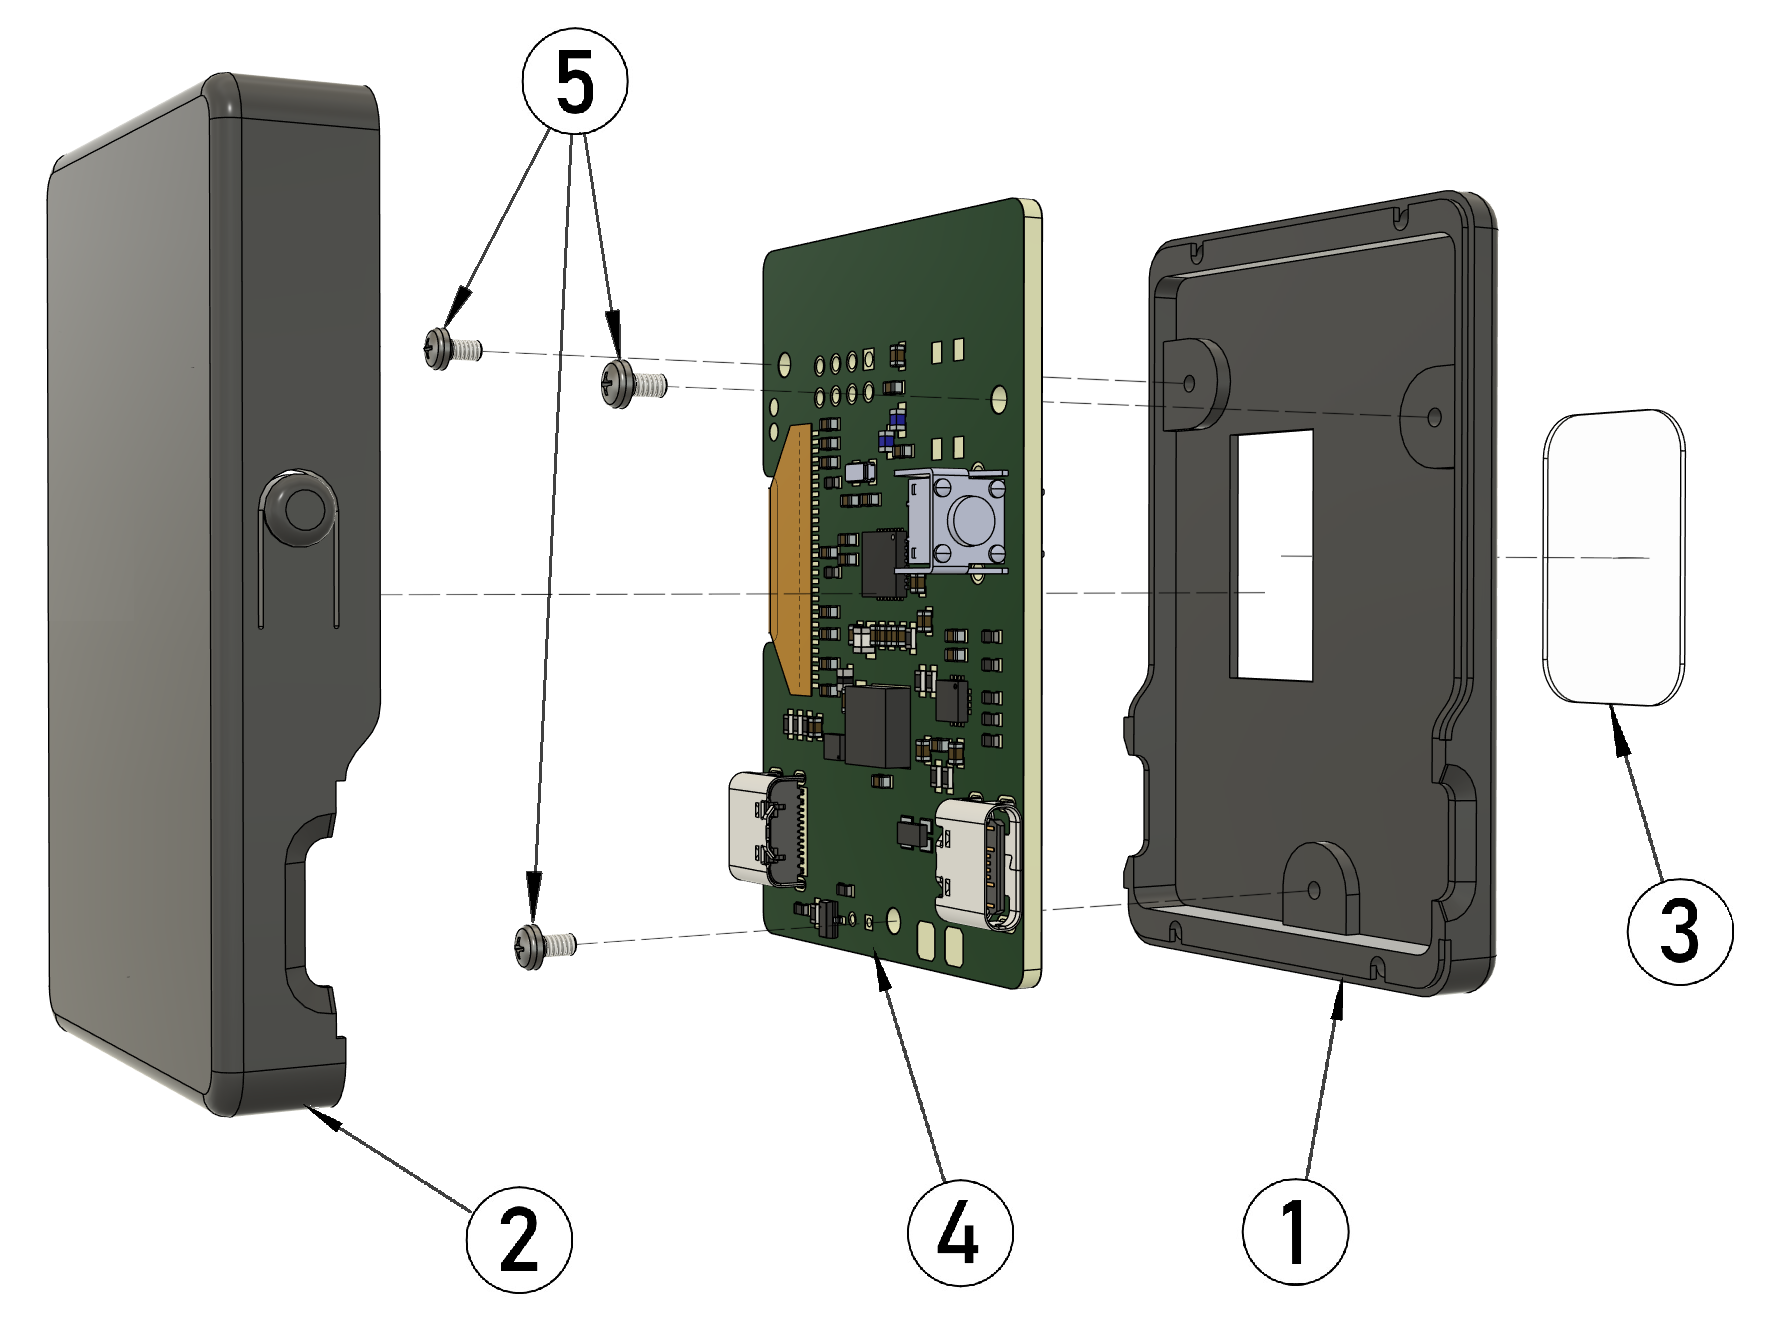
\includegraphics[width=0.9\textwidth]{figures/mech_assembly.png}
    \caption{Exploded 3D view of the system's mechanical assembly.}
    \label{fig:mech_exploded}
\end{figure}

\begin{table}[H]
    \centering
    \renewcommand{\arraystretch}{1.4}
    \caption{Description of the primary mechanical assembly components.}
    \label{tab:mech_components}
    
    \begin{tabularx}{\textwidth}{|c|l|X|}
    \hline
    \textbf{No.} & \textbf{Name} & \textbf{Description} \\
    \hline
    
    \textbf{1} & Top Cover & Upper half of the protective enclosure. \\
    \hline
    
    \textbf{2} & Bottom Cover & Bottom half of the protective enclosure. \\
    \hline

    \textbf{3} & Screen Cover & Clear cover for the device display. \\
    \hline

    \textbf{4} & PCB & The production version of the 4-layer Printed Circuit Board.. \\
    \hline

    \textbf{5} & Mounting Screws & Three M1.6 x 3 screws used to secure the pcb on the top cover \\
    \hline        
    
\end{tabularx}
\end{table}


\subsection{External Interfaces and Connectivity}

Figure~\ref{fig:mech_interface} illustrates the fully assembled device, with its primary external interfaces and ports detailed in Table~\ref{tab:user_interface}.


\begin{figure}[H]
    \centering
    % Update the filename/path if necessary
    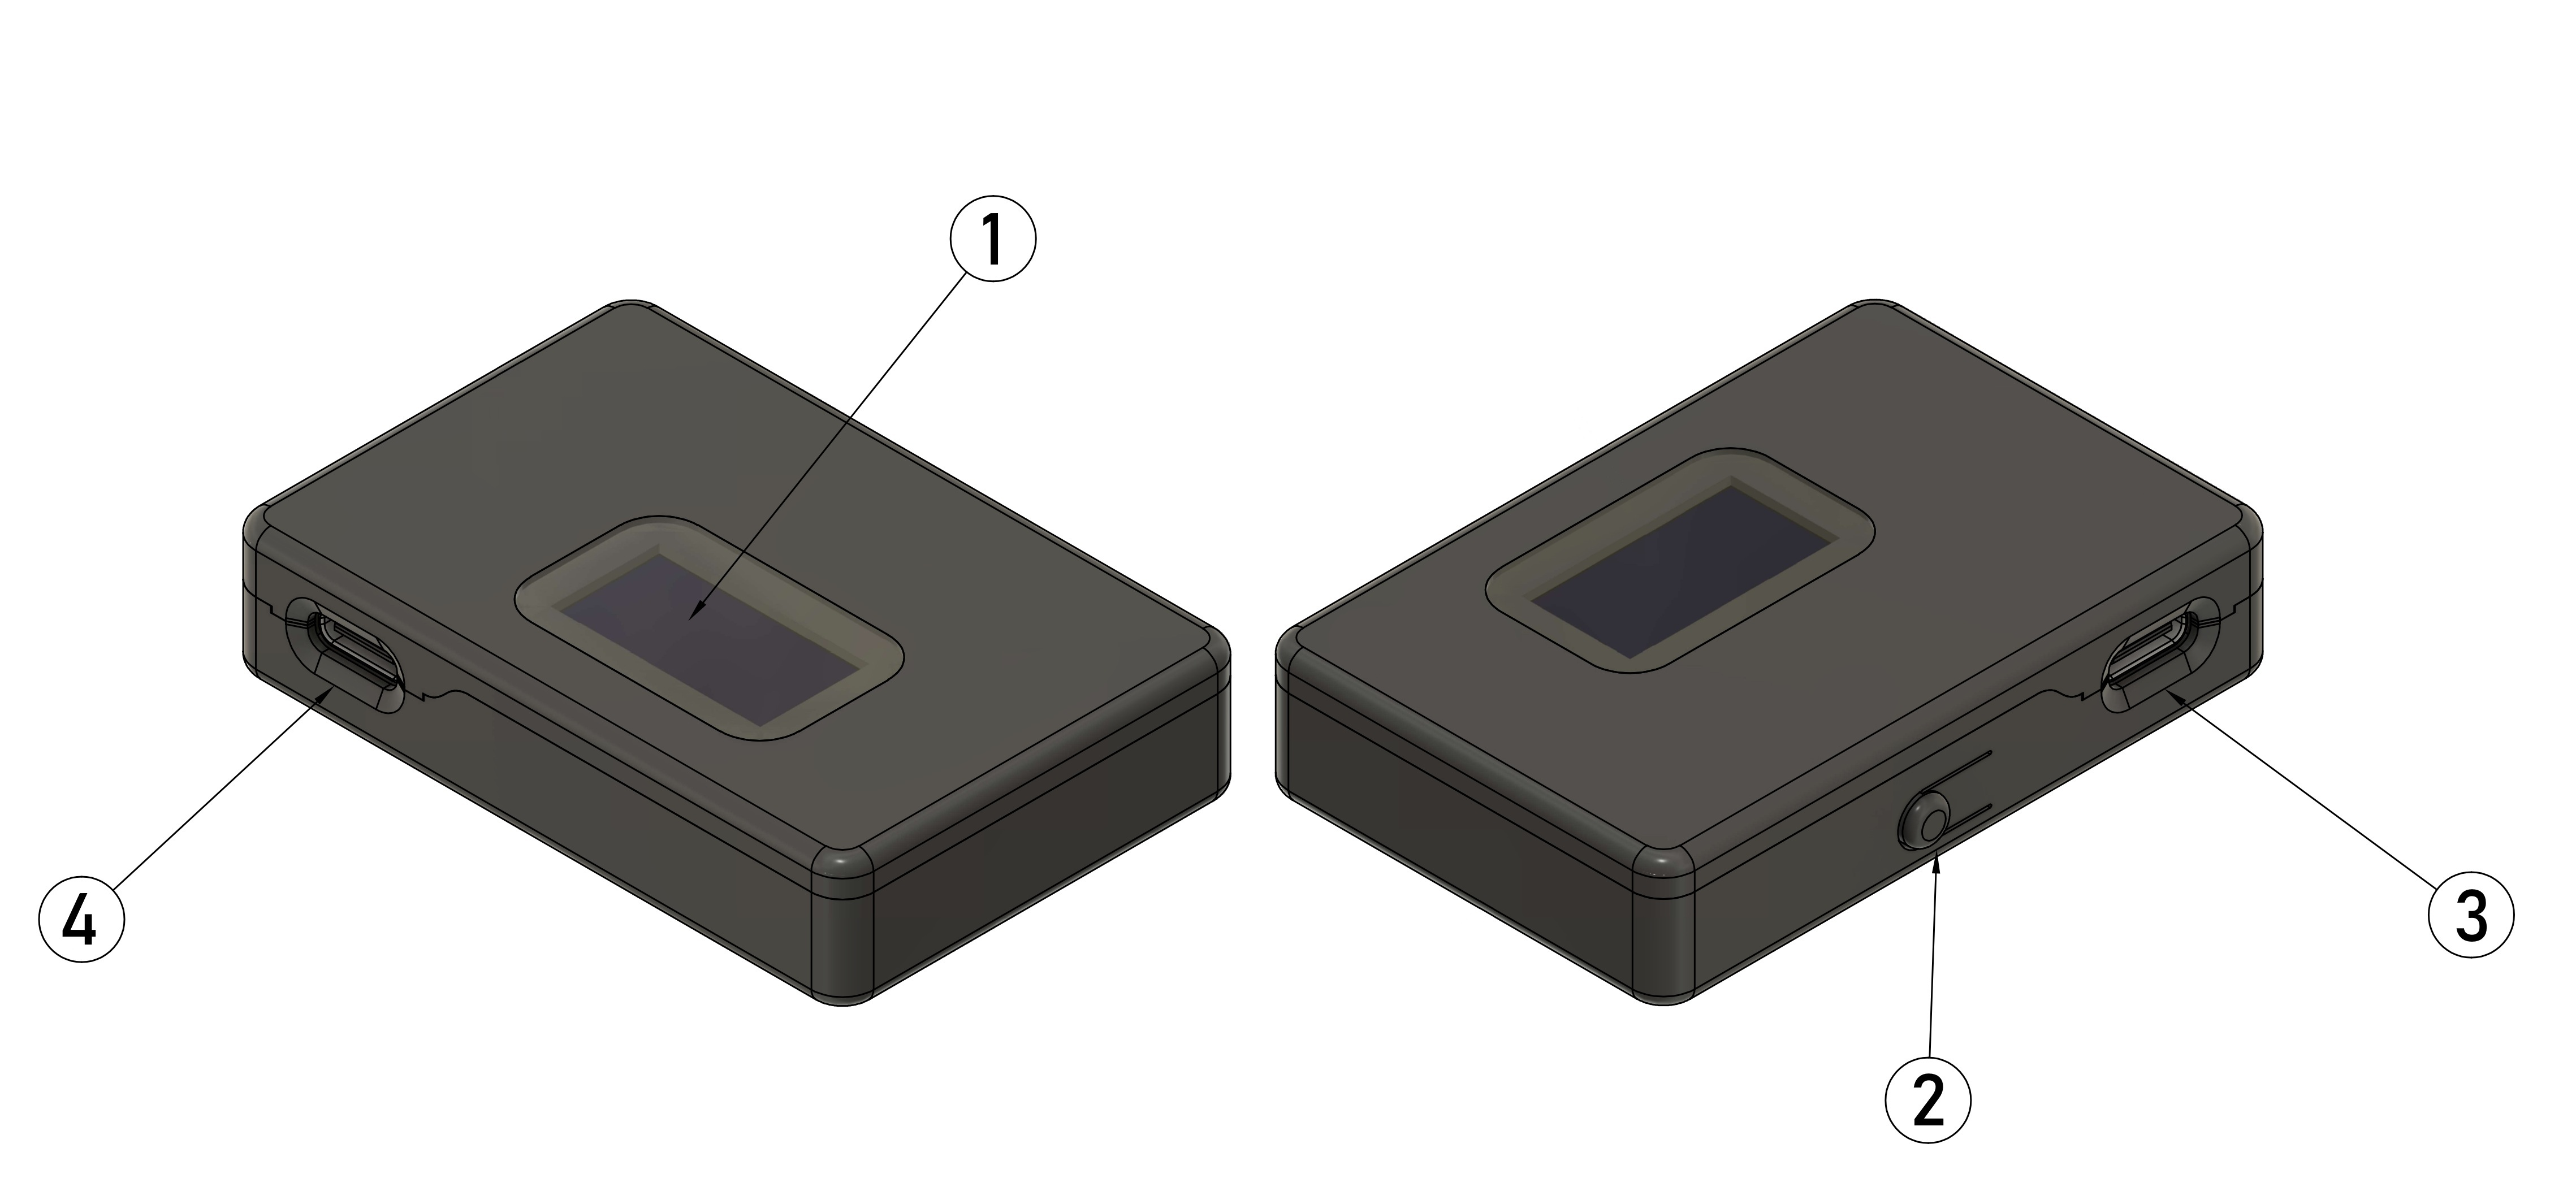
\includegraphics[width=\textwidth]{figures/mech_components.jpg}
    \caption{External view of the fully assembled system highlighting the key user interfaces and connectivity.}
    \label{fig:mech_interface}
\end{figure}


\begin{table}[H]
    \centering
    \renewcommand{\arraystretch}{1.4}
    \caption{Description of the external interfaces.}
    \label{tab:user_interface}
    
    \begin{tabularx}{\textwidth}{|c|l|X|}
        \hline
        \textbf{No.} & \textbf{Name} & \textbf{Description} \\
        \hline

        \textbf{1} & Display & Device display accessible through the enclosure cutout. \\
        \hline

        \textbf{2} & Button Actuator & User button actuator directly embedded in the protective enclosure. \\
        \hline

        \textbf{3} & Input Port & Power port connected to the powerbank or power source. \\
        \hline

        \textbf{4} & Output Port & Power port connected to the loaded device or battery charger. \\
        \hline
        
    \end{tabularx}
\end{table}

%--------------------------------------------------

% Project Management
\chapter{Manufacturing and \mbox{Assembly}}

\section{Manufacturer Report}

The PCB design was entirely developed targeting JLCPCB manufacturing capabilities, with the explicit objective of minimizing production cost while still satisfying all electrical, thermal, and mechanical system requirements. Since the performance requirements of the system do not impose high-frequency or high-power constraints beyond standard low-cost fabrication capabilities, no design choices were made that would require higher-tier manufacturing processes. For this reason, routing rules, via usage, stack-up selection, and component spacing were all optimized according to JLCPCB lowest-cost production class, where constraints are primarily driven by minimum trace width, minimum via diameter, and via-to-via spacing rather than absolute via density.

Eurocircuits manufacturing tools were subsequently used as an additional validation step. However, this introduced an apparent discrepancy in the cost assessment: via density becomes a penalizing factor in the Eurocircuits manufacturing model, causing the drill classification to increase from Class C to Class E. This increase is not driven by limitations of the manufacturing process itself, but rather by the large number of vias employed throughout the design for grounding, thermal management, and signal integrity purposes. In contrast, within the intended JLCPCB manufacturing environment, the same design remains fully compliant with the lowest-cost category, since via density does not directly affect pricing as long as spacing constraints are respected.

\begin{figure}[H]
    \centering
    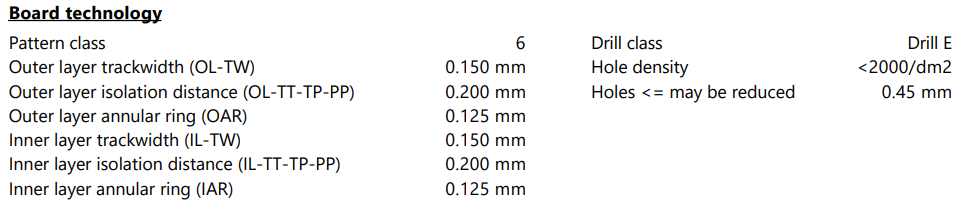
\includegraphics[width=0.9\textwidth]{figures/eurocircuits_report.png}
    \caption{Eurocircuits manufacturing analysis report showing the PCB production classification and drill category.}
    \label{fig:eurocircuits_report}
\end{figure}

\begin{landscape}

    \section{BOM and Costs}

    \small                          % slightly smaller font to fit columns

    \begin{longtable}{
        |c                          % Item
        |p{3cm}                   % Reference
        |c                   % Value
        |p{5cm}                   % MPN
        |l                   % Description
        |c                          % Qty
        |p{1.2cm}                          % Cost 1x
        |p{1.2cm}                          % Cost 10x
        |p{1.2cm}|                         % Cost 100k
    }

        % ---------------------------------------------------------------
        %  CAPTION (shown once at the top of the first page)
        % ---------------------------------------------------------------
        \caption{Bill of Materials with Cost Breakdown}
        \label{tab:bom}\\

        % ---------------------------------------------------------------
        %  HEADER (repeated at the top of every page)
        % ---------------------------------------------------------------
        \hline
        \rowcolor[gray]{0.85}
        \textbf{Item} &
        \textbf{Reference} &
        \textbf{Value} &
        \textbf{MPN} &
        \textbf{Description} &
        \textbf{Qty} &
        \textbf{Cost 1x} &
        \textbf{Cost 10x} &
        \textbf{Cost 100k} \\
        \hline
        \endfirsthead

        \multicolumn{9}{l}{\small\itshape (continued from previous page)}\\[2pt]
        \hline
        \rowcolor[gray]{0.85}
        \textbf{Item} &
        \textbf{Reference} &
        \textbf{Value} &
        \textbf{MPN} &
        \textbf{Description} &
        \textbf{Qty} &
        \textbf{Cost 1x} &
        \textbf{Cost 10x} &
        \textbf{Cost 100k} \\
        \hline
        \endhead

        % ---------------------------------------------------------------
        %  FOOTER (every page except the last)
        % ---------------------------------------------------------------
        \hline
        \multicolumn{9}{r}{\small\itshape (continued on next page)}\\
        \endfoot

        % ---------------------------------------------------------------
        %  LAST FOOTER
        % ---------------------------------------------------------------
        \hline\hline

% ---------------- COMPONENTS ----------------
\multicolumn{5}{|r|}{\textbf{Total for Components}} &
\multicolumn{1}{c|}{ } &
\textbf{28.74\,\euro} &
\textbf{22.18\,\euro} &
\textbf{8.86\,\euro} \\
\hline

% ---------------- PCB ----------------
\multicolumn{5}{|r|}{PCB Manufacturing} &
\multicolumn{1}{c|}{ } &
1.20\,\euro &
1.12\,\euro &
0.16\,\euro \\
\hline

% ---------------- ASSEMBLY BREAKDOWN ----------------
\multicolumn{5}{|r|}{PCB Assembly \textsuperscript{(2)} }&
\multicolumn{1}{c|}{ } &
0.49\,\euro &
0.49\,\euro &
0.33\,\euro  \\
\hline

% ---------------- TOTAL MANUFACTURING ----------------
\multicolumn{5}{|r|}{\textbf{Total for Manufacturing}} &
\multicolumn{1}{c|}{ } &
\textbf{1.69\,\euro} &
\textbf{1.61\,\euro} &
\textbf{0.49\,\euro} \\
\hline

% ---------------- ENCLOSURE ----------------
\multicolumn{5}{|r|}{3D Printed Enclosure \textsuperscript{(2)} } &
\multicolumn{1}{c|}{ } &
0.94\,\euro &
0.94\,\euro &
0.94\,\euro \textsuperscript{(3)}\\
\hline

% ---------------- GRAND TOTAL ----------------
\multicolumn{5}{|r|}{\textbf{Grand Total}} &
\multicolumn{1}{c|}{ } &
\textbf{31.36\,\euro} &
\textbf{24.72\,\euro} &
\textbf{10.29\,\euro} \\
\hline

\endlastfoot

        % ---------------------------------------------------------------
        %  DATA ROWS
        % ---------------------------------------------------------------
        1  & A1 & -- & --
        & PCB Inverted F Antenna 2--4\,GHz & 1
        & -- & -- & -- \\
        \hline

        2  & C1, C2, C3, C6, C7, C11, C16, C20, C22, C23, C25, C28, C29
        & 100\,n & 0603B104K500CT
        & Cap 0.1\,\textmu F, 50\,V, X7R, 10\%, 0603 & 13
        & 0.09\,\euro & 0.02\,\euro & 0.00\,\euro \\
        \hline

        3  & C4, C5, C8 & 10\,\textmu & 0603X106M6R3CT
        & Cap 10\,\textmu F, 6.3\,V, X5R, 20\%, 0603 & 3
        & 0.09\,\euro & 0.03\,\euro & 0.01\,\euro \\
        \hline

        4  & C9, C10, C12 & 12\,p & 0603N120J500CT
        & Cap 12\,pF, 50\,V, C0G NP0, 5\%, 0603 & 3
        & 0.09\,\euro & 0.02\,\euro & 0.00\,\euro \\
        \hline

        5  & C13, C14 & 1.2\,p & CC0603BRNPO9BN1R2
        & Cap 1.2\,pF, 50\,V, C0G NP0, $\pm$0.1\,pF, 0603 & 2
        & 0.09\,\euro & 0.05\,\euro & 0.01\,\euro \\
        \hline

        6  & C15, C24, C27 & 2.2\,\textmu & 0603X225K160CT
        & Cap 2.2\,\textmu F, 16\,V, 10\%, 0603 & 3
        & 0.09\,\euro & 0.03\,\euro & 0.01\,\euro \\
        \hline

        7  & C17, C19 & 470\,n & MCASU168SB5474KTNA01
        & Cap 0.47\,\textmu F, X5R, 10\%, 0603 & 2
        & 0.12\,\euro & 0.07\,\euro & 0.00\,\euro \\
        \hline

        8  & C18 & 4.7\,\textmu & GMC10X5R475K6R3NT
        & Cap 4.7\,\textmu F, 6.3\,V, X5R, 10\%, 0603 & 1
        & 0.09\,\euro & 0.03\,\euro & 0.01\,\euro \\
        \hline

        9  & C21, C26, C32 & 1\,\textmu & 0603B105K250CT
        & Cap 1\,\textmu F, 25\,V, X7R, 10\%, 0603 & 3
        & 0.09\,\euro & 0.02\,\euro & 0.00\,\euro \\
        \hline

        10 & C30 & 4.7\,\textmu & GRM219R6YA475KA73J
        & Cap 4.7\,\textmu F, 35\,V, X5R, 10\%, 0805, 4.8\,m$\Omega$ & 1
        & 0.14\,\euro & 0.08\,\euro & 0.02\,\euro \\
        \hline

        11 & C31 & 47\,\textmu & GRM21BR61A476ME15L
        & Cap 47\,\textmu F, 10\,V, X5R, 20\%, 0805, 0.18\,m$\Omega$ & 1
        & 0.46\,\euro & 0.28\,\euro & 0.11\,\euro \\
        \hline

        12 & IC1 & -- & PAC1951T-1E/4MX
        & IC Current/Voltage Monitor, 1\%, 16\,VQFN & 1
        & 1.00\,\euro & 0.83\,\euro & 0.81\,\euro \\
        \hline

        13 & IC2 & -- & MAX77597ETBB+T
        & 36\,V, 300\,mA Buck Converter, 1.1\,\textmu A $I_q$ & 1
        & 1.65\,\euro & 1.21\,\euro & 0.81\,\euro \\
        \hline

        14 & J1 & -- & MCOT128064N2Z-BM
        & MCOT128064N2Z-BM Display & 1
        & 11.37\,\euro & 10.92\,\euro & 2.11\,\euro \\
        \hline

        15 & J2, J3 & -- & USB4215-03-A
        & USB-C Connector, 5\,A & 2
        & 0.45\,\euro & 0.37\,\euro & 0.23\,\euro \\
        \hline

        16 & J4 & -- & PR20204VBDN
        & Pin Header, 4$\times$2, 2.54\,mm pitch, TH & 1
        & 0.09\,\euro & 0.05\,\euro & 0.03\,\euro \\
        \hline

        17 & L1 & 10\,u & LQM21FN100M80L
        & Ind 10\,\textmu H, 100\,mA, 20\%, 0805 & 1
        & 0.16\,\euro & 0.14\,\euro & 0.07\,\euro \\
        \hline

        18 & L2 & 15\,n & LQG18HN15NJ00D
        & Ind 15\,nH, 600\,mA, 0603, 400\,m$\Omega$ & 1
        & 0.14\,\euro & 0.11\,\euro & 0.06\,\euro \\
        \hline

        19 & L5 & 2.2\,n & LQG18HN2N2S00D
        & Ind 2.2\,nH, 1.1\,A, 0603, 100\,m$\Omega$ & 1
        & 0.14\,\euro & 0.11\,\euro & 0.06\,\euro \\
        \hline

        20 & L6 & 47\,\textmu & ASPI-0615FS-470M-T2
        & Ind 47\,\textmu H, 800\,mA, 370\,m$\Omega$ & 1
        & 0.30\,\euro & 0.25\,\euro & 0.13\,\euro \\
        \hline

        21 & L7 & 1.5\,k & BLM18HE152SN1D
        & Ferrite Bead 1.5\,k$\Omega$, 500\,mA, 0603 & 1
        & 0.19\,\euro & 0.13\,\euro & 0.04\,\euro \\
        \hline

        22 & MH1, MH2, MH3 & -- & --
        & M2 Mounting Hole & 3
        & -- & -- & -- \\
        \hline

        23 & Q1 & -- & SI2365EDS-T1-BE3
        & MOSFET SOT-23 P-Ch, 20\,V, 4.5\,A & 1
        & 0.40\,\euro & 0.24\,\euro & 0.06\,\euro \\
        \hline

        24 & RT1 & -- & 103AP-2
        & NTC Thermistor, 10\,k$\Omega$, 0.5\% & 1
        & 0.60\,\euro & 0.50\,\euro & 0.33\,\euro \\
        \hline

        25 & R1, R6, R7, R8, R16 & 10\,k & WR06X103 JTL
        & Res 10\,k$\Omega$, 0603, 5\%, 0.1\,W & 5
        & 0.09\,\euro & 0.01\,\euro & 0.00\,\euro \\
        \hline

        26 & R2, R13, R18, R19 & 100\,k & WR06X104 JTL
        & Res 100\,k$\Omega$, 0603, 5\%, 0.1\,W & 4
        & 0.09\,\euro & 0.01\,\euro & 0.00\,\euro \\
        \hline

        27 & R3, R4, R14 & 1\,k & WR06X102 JTL
        & Res 1\,k$\Omega$, 0603, 5\%, 0.1\,W & 3
        & 0.09\,\euro & 0.01\,\euro & 0.00\,\euro \\
        \hline

        28 & R5, R9 & 0\,$\Omega$ & WR06X000 PTL
        & Res 0\,$\Omega$, 0603 & 2
        & 0.09\,\euro & 0.01\,\euro & 0.00\,\euro \\
        \hline

        29 & R10 & 10\,m & LVK12R010CER
        & Res 10\,m$\Omega$, 1206, 0.25\%, 0.5\,W & 1
        & 1.31\,\euro & 0.86\,\euro & 0.34\,\euro \\
        \hline

        30 & R11, R12 & 32.4\,$\Omega$ & RMCF0603FT32R4
        & Res 32.4\,$\Omega$, 0603, 1\%, 0.1\,W & 2
        & 0.09\,\euro & 0.02\,\euro & 0.00\,\euro \\
        \hline

        31 & R15 & 5.76\,k & ERA3AEB5761V
        & Res 5.76\,k$\Omega$, 0603, 0.1\%, 0.1\,W & 1
        & 0.09\,\euro & 0.05\,\euro & 0.03\,\euro \\
        \hline

        32 & R17 & 402\,k & RMCF0603FT402K
        & Res 402\,k$\Omega$, 0603, 1\%, 0.1\,W & 1
        & 0.09\,\euro & 0.02\,\euro & 0.00\,\euro \\
        \hline

        33 & R20 & 240\,k & MCR03ERTJ244
        & Res 240\,k$\Omega$, 0603, 5\%, 0.1\,W & 1
        & 0.10\,\euro & 0.01\,\euro & 0.00\,\euro \\
        \hline

        34 & S1 & -- & TS11-674-43-BK-260-RA-D
        & SPST Tactile Switch, TH & 1
        & 0.14\,\euro & 0.12\,\euro & 0.08\,\euro \\
        \hline

        35 & S2 & -- & TL3305CF260QG
        & SPST Tactile Switch, SMD & 1
        & 0.18\,\euro & 0.15\,\euro & 0.09\,\euro \\
        \hline

        36 & TP1--TP7 & -- & --
        & Test Point & 7
        & -- & -- & -- \\
        \hline

        37 & U1 & -- & CC2640R2FRHBR
        & IC RF TxRx + MCU Bluetooth, 32-VFQFN & 1
        & 3.92\,\euro & 3.39\,\euro & 2.47\,\euro \\
        \hline

        38 & Y1 & -- & TSX-3225240000MF15X-AC3
        & Crystal 24\,MHz, 9\,pF, 10\,ppm & 1
        & 0.71\,\euro & 0.61\,\euro & 0.44\,\euro \\
        \hline

        39 & Y2 & -- & FC-135R 32.7680KA-AG0
        & Crystal 32.768\,kHz, 7\,pF, 20\,ppm & 1
        & 0.46\,\euro & 0.40\,\euro & 0.27\,\euro \\

    \end{longtable}

\vspace{0.2cm}
\noindent\footnotesize
\textit{1:} IVA is not included in the calculated costs.\\
\textit{2:} Values are estimated by cost calculator tools provided JLCPCB Manufacturer.\\
\textit{3:} For large-scale production, injection molding is preferred over 3D printing for the plastic cover.


\end{landscape}

%--------------------------------------------------

% Project Management


\begin{landscape}

    \chapter{Project Management}
    \section{Development Timeline (GANTT)}

        \begin{ganttchart}[
        %--- grid ---
        hgrid style/.style       = {draw=white, line width=0.9pt},
        vgrid                    = {*3{draw=white!60, line width=0.35pt},
                                    {draw=white,     line width=0.9pt}},
        %--- canvas ---
        canvas/.style            = {fill=canvasbg!55, draw=none},
        %--- title (month header) ---
        title/.style             = {fill=titlebg, draw=none},
        title label font         = \bfseries\color{white}\small,
        include title in canvas  = false,
        %--- group rows (Hardware / Firmware / Testing) ---
        group/.style             = {fill=catred, draw=none},
        group label font         = \bfseries\small\color{black},
        group label anchor/.style= {left=3pt},
        group peaks width        = {0},
        group peaks height       = {0},
        group height             = 0.55,
        %--- task bars ---
        bar/.style               = {fill=barblue, draw=none, rounded corners=1.5pt},
        bar height               = 0.5,
        bar label font           = \footnotesize,
        bar label anchor/.style  = {left=3pt},
        %--- sizing ---
        x unit                   = 0.68cm,
        y unit title             = 0.68cm,
        y unit chart             = 0.60cm,
        ]{1}{28}

        %=== Year headers =========================================================
        \gantttitle{2025}{4}
        \gantttitle{2026}{24} \\

        %=== Month headers (4 slots × 7 months = 28 slots) =======================
        \gantttitle{December}{4}
        \gantttitle{January}{4}
        \gantttitle{February}{4}
        \gantttitle{March}{4}
        \gantttitle{April}{4}
        \gantttitle{May}{4}
        \gantttitle{June}{4} \\

        %=== HARDWARE =============================================================
        \ganttgroup{Hardware}{1}{21} \\

        % Slots: Dec=1-4, Jan=5-8, Feb=9-12, Mar=13-16, Apr=17-20, May=21-24, Jun=25-28
        \ganttbar{Preliminary Analysis \& Presentation}{1}{2} \\
        \ganttbar{Final HW Requirements Definition}{11}{12} \\
        % Two bars on the same row (Dec prototype + Feb revision)
        \ganttbar{Component selection}{1}{2}
        \ganttbar[bar/.style={fill=barblue,draw=none,rounded corners=1.5pt}]{}{11}{12} \\
        \ganttbar{Schematics drawing}{12}{14} \\
        \ganttbar{PCB Layout \& Routing}{14}{19} \\
        \ganttbar{Hardware check \& final BOM}{18}{19} \\
        \ganttbar{PCB Manufacturing \& Assembly}{20}{21} \\

        %=== FIRMWARE =============================================================
        \draw[thick, dashed] (current bounding box.west |- 0,-6.2) -- (current bounding box.east |- 0,-6.2);
        \ganttgroup{Firmware}{13}{25} \\

        \ganttbar{Getting familiar with TI Software}{13}{14} \\
        \ganttbar{Firmware Drivers (Sensor, BLE, \dots)}{14}{16} \\
        \ganttbar{Components Integration \& Algorithm}{15}{23} \\
        \ganttbar{Firmware Refinements and Debug}{22}{25} \\
        \ganttbar{Android APP Implementation}{18}{22} \\

        %=== TESTING ==============================================================
        \draw[thick, dashed] (current bounding box.west |- 0,-9.8) -- (current bounding box.east |- 0,-9.8);
        \ganttgroup{Testing}{21}{25} \\

        \ganttbar{Hardware Functionality Tests}{21}{22} \\
        \ganttbar{HW-SW Integration Tests \& Debug}{22}{23} \\
        \ganttbar{Full System Test \& Debug (w.\ APP)}{24}{25}

    \end{ganttchart}

\end{landscape}

%--------------------------------------------------
\appendix

\begin{landscape}
  \chapter{Schematics}
  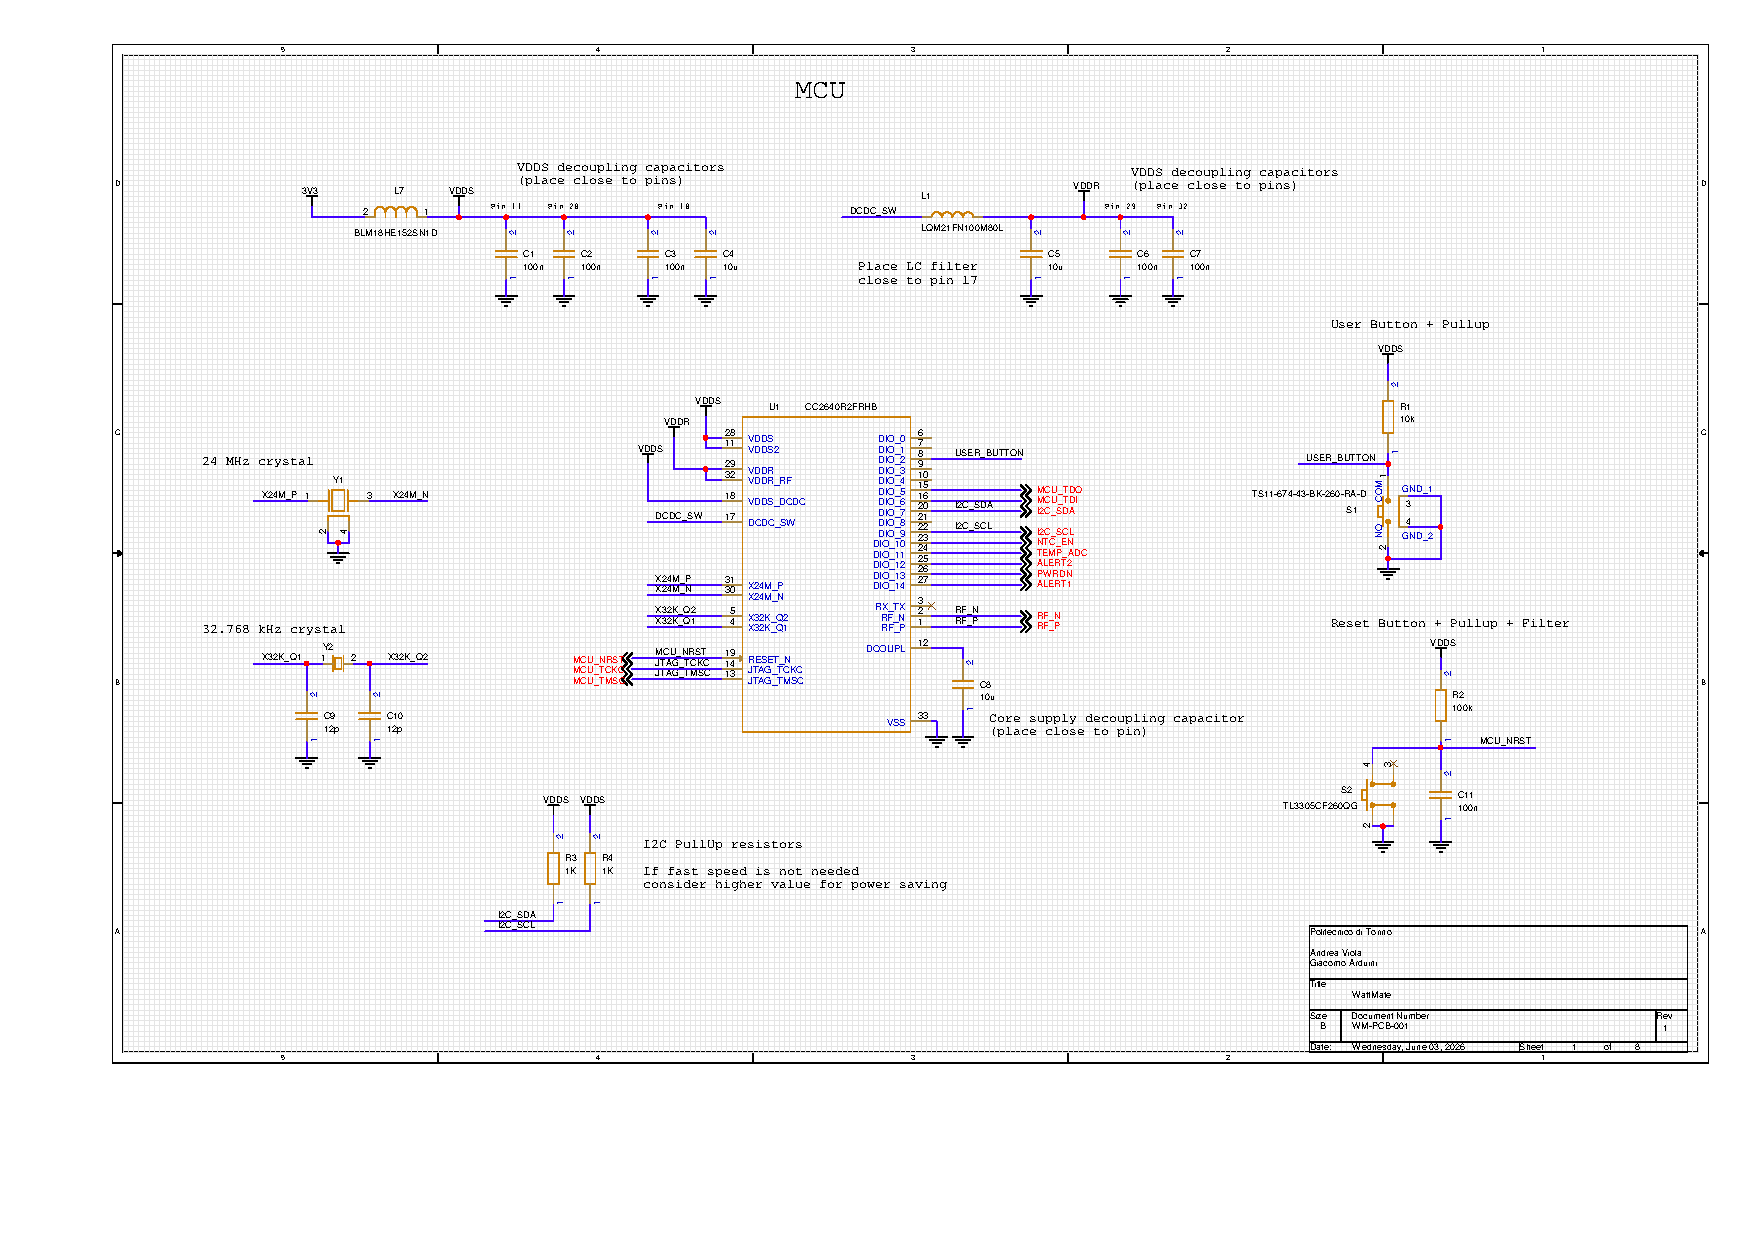
\includepdf[pages=-, angle=90]{appendix/WM-PCB-001_Schematics.pdf}
\end{landscape}

\chapter{PCB Layout}
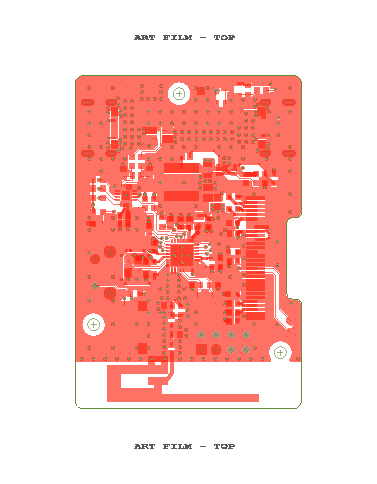
\includepdf[pages=-]{appendix/WM-PCB-001_Layout.pdf}

\begin{landscape}
  \chapter{PCB Dimensions}
  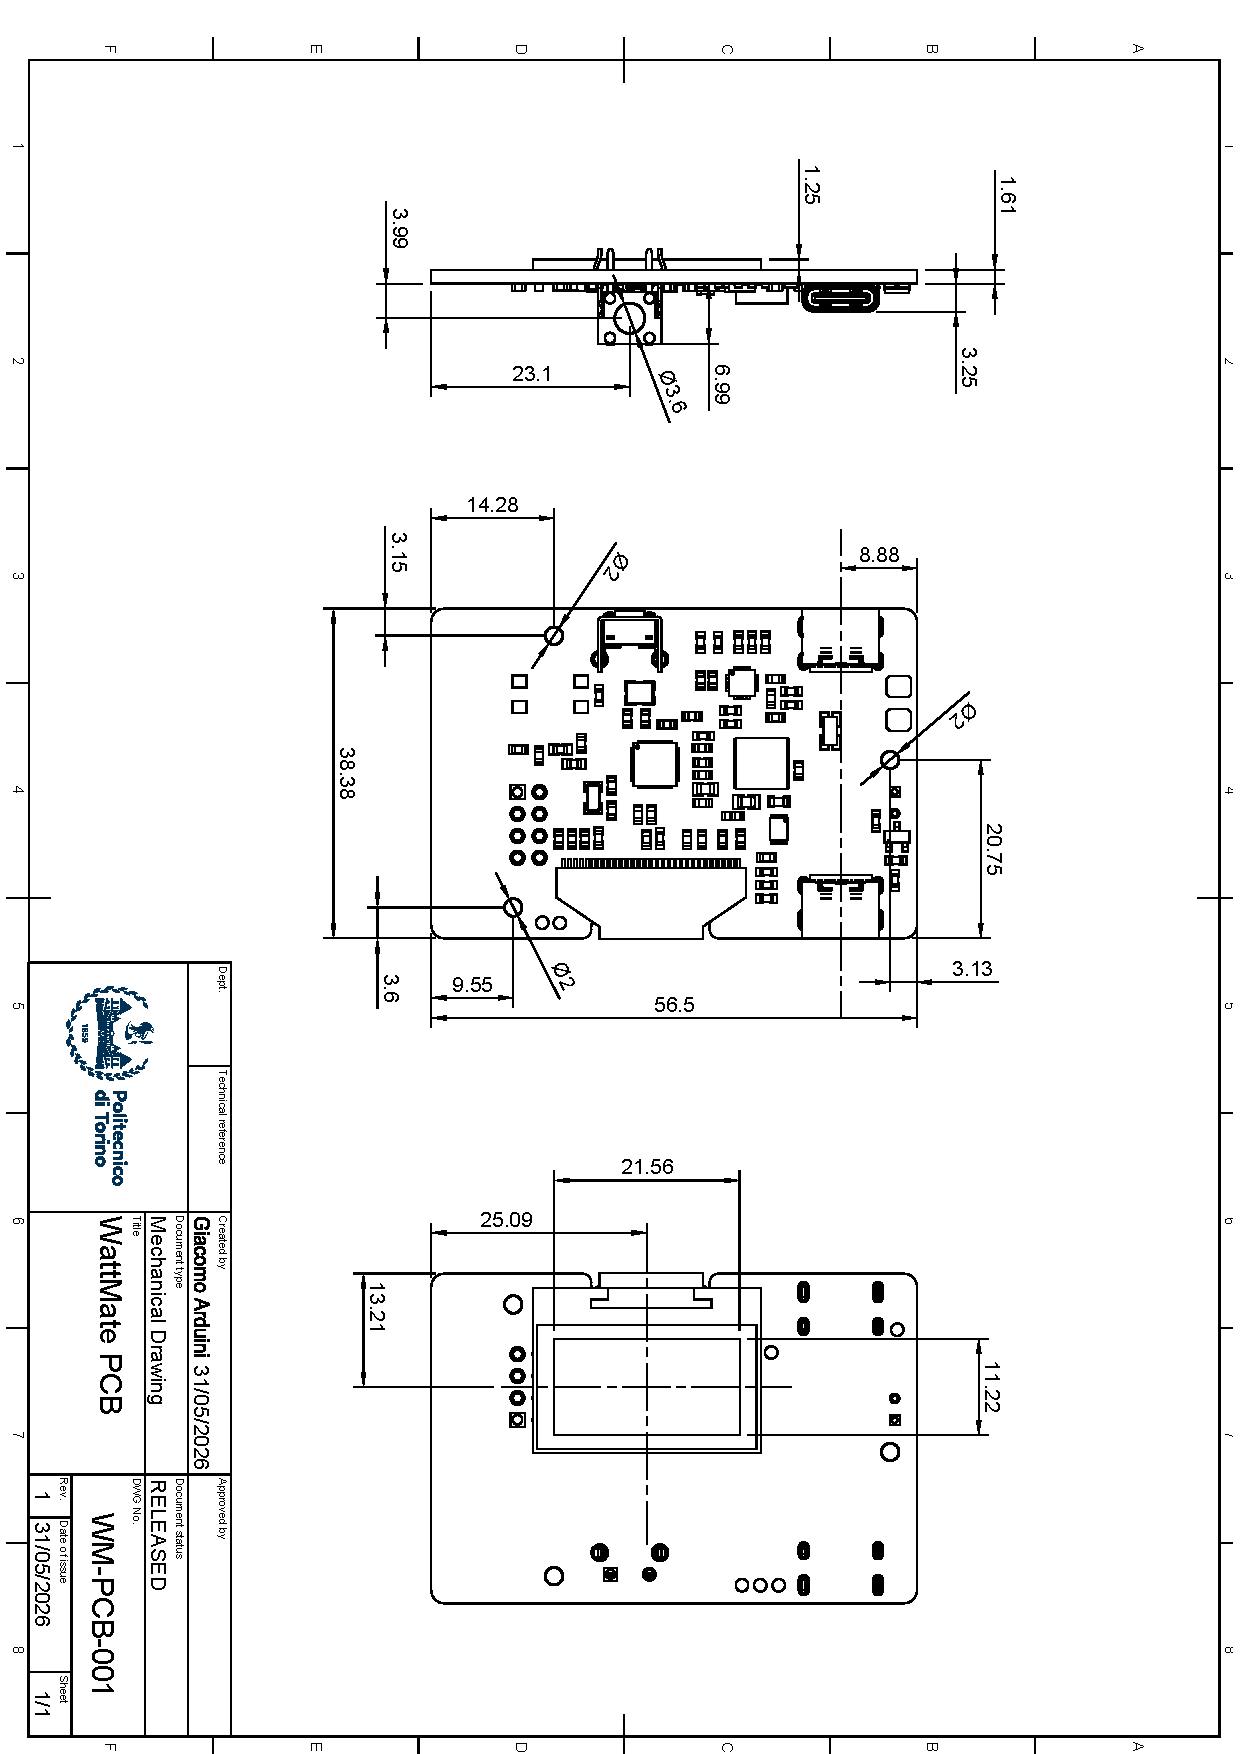
\includepdf[pages=-, angle=180]{appendix/WM-PCB-001_Drawing.pdf}
\end{landscape}

\begin{landscape}
  \chapter{Enclosure Dimensions}
  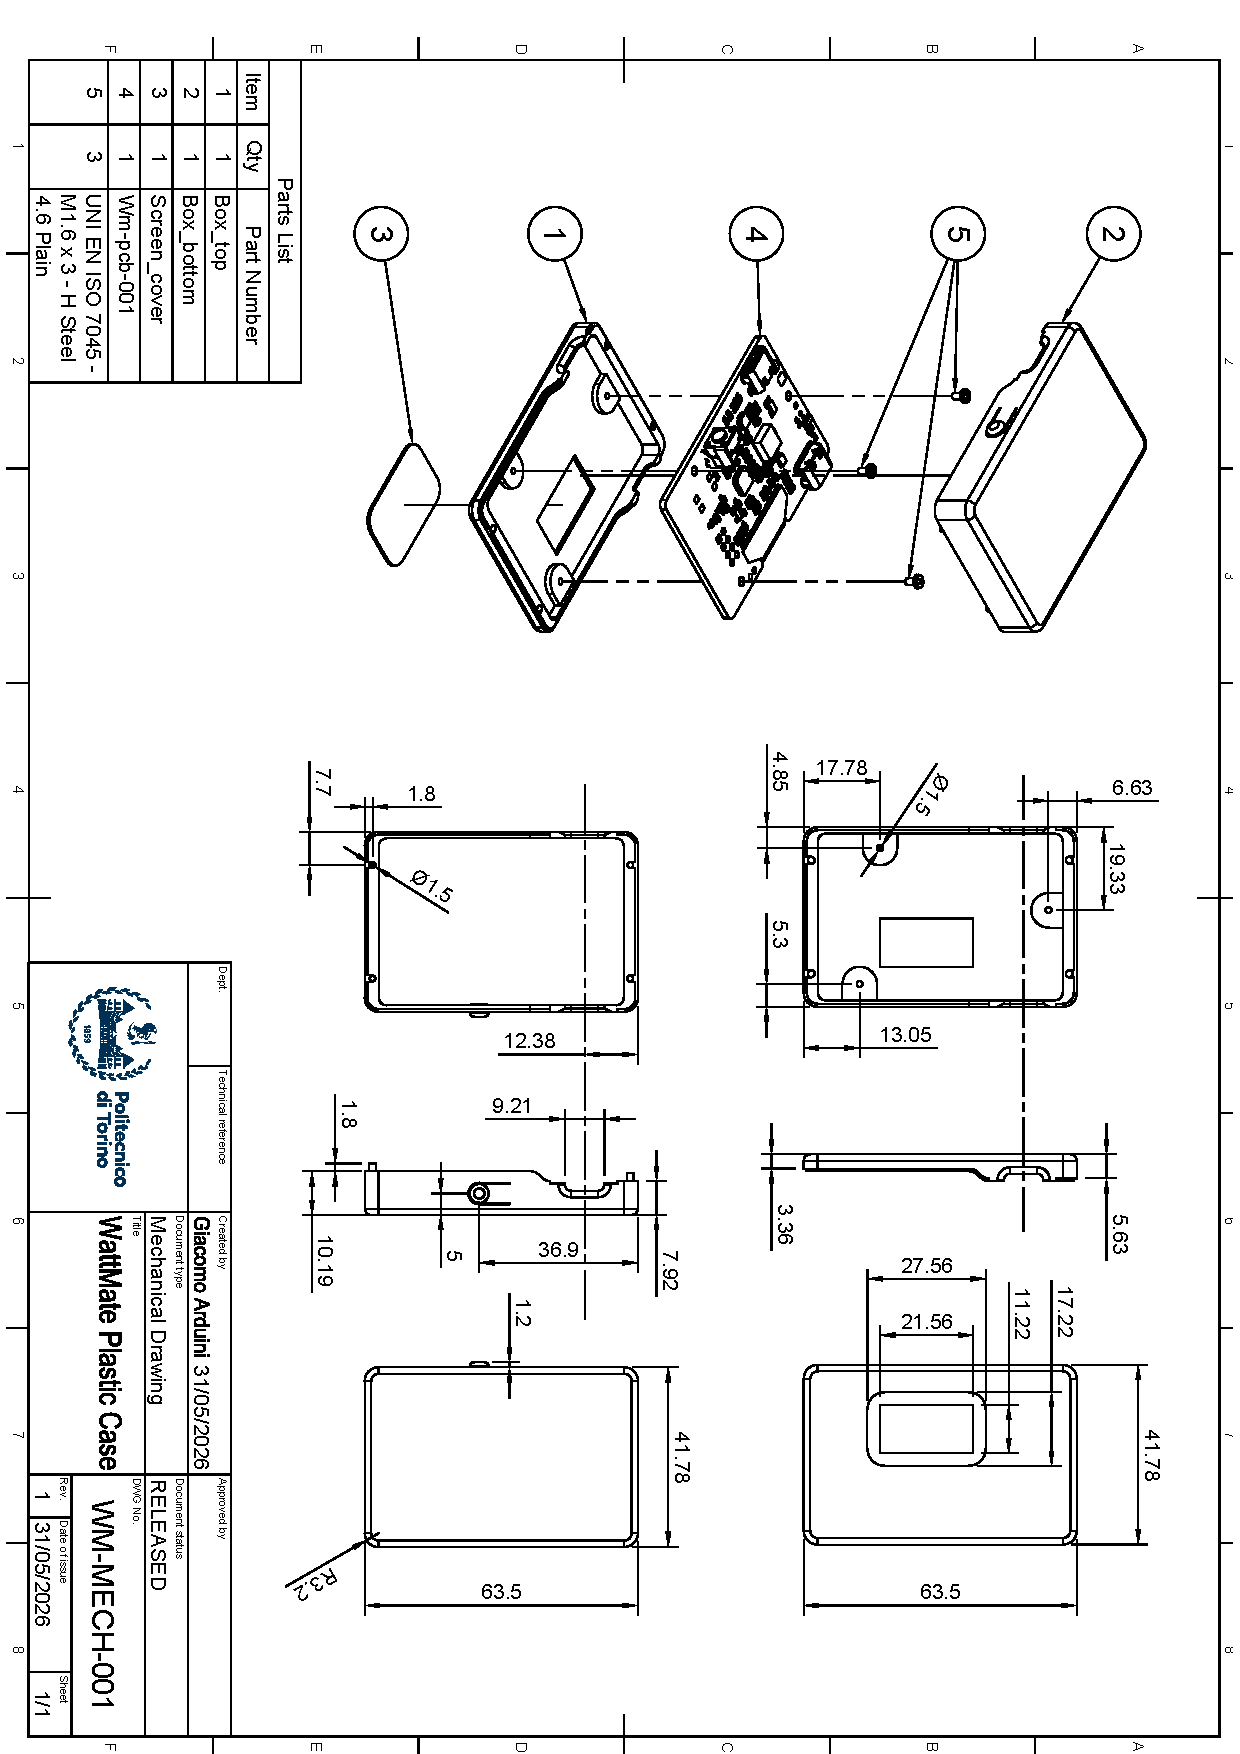
\includepdf[pages=-, angle=180]{appendix/WM-MECH-001_Drawing.pdf}
\end{landscape}

% Print all bibliography entries, even if not cited
\nocite{*}

% Print bibliography and add it to the table of contents
\printbibliography[heading=bibintoc, title={Bibliography}]

\end{document}